\documentclass[a4paper, twoside, 12pt]{report}

%% Language and font encodings
\usepackage{amsmath}
\usepackage{titling}
\usepackage[english]{babel}
\usepackage[utf8x]{inputenc}
\usepackage[T1]{fontenc}
\usepackage{tikz-feynman}
\usepackage{subcaption}
\usepackage{graphicx}
\usepackage{caption}
\usepackage{float}
\usepackage{graphicx,booktabs,array}
\usepackage{array,multirow}
\usepackage{adjustbox}
\usepackage{enumerate}

%% Sets page size and margins
\usepackage[a4paper,top=3cm,bottom=2cm,left=3cm,right=3cm,marginparwidth=1.75cm]{geometry}
\usepackage{array}
\renewcommand{\baselinestretch}{1.3} 
\newcolumntype{x}[1]{>{\centering\arraybackslash\hspace{0pt}}m{#1}}
\newcommand{\addpic}{\includegraphics[width=6em]{example-image}}
\newcolumntype{C}{>{\centering\arraybackslash}m{16em}}
\setlength\parindent{0pt}

%% Useful packages
\usepackage{amsmath}
\usepackage{amssymb}
\usepackage{graphicx}
\usepackage[colorinlistoftodos]{todonotes}
\usepackage[colorlinks=true, allcolors=blue]{hyperref}
\usepackage{fancyhdr}

\pagestyle{fancy}
\fancyhead{} % clear all header fields
\fancyhead[LE, RO]{\thepage}
\fancyhead[LO, RE]{\leftmark}
\fancyfoot{}
\renewcommand{\chaptermark}[1]{%
\markboth{#1}{}}

\newcommand{\tauh}{\tau_{h}}
\newcommand{\tauhtauh}{\tau_{h}\tau_{h}}
\newcommand{\mutauh}{\mu_{}\tau_{h}}
\newcommand{\etauh}{e_{}\tau_{h}}
\newcommand{\emu}{e_{}\mu_{}}
\newcommand{\mumu}{\mu_{}\mu_{}}
\newcommand{\ee}{e_{}e_{}}
\newcommand{\lag}{\mathcal{L}}

\title{Searches for New Physics With Tau Leptons at the CMS Experiment}
\author{George Uttley}

\begin{document}
%\begin{titlepage}

\newcommand{\HRule}{\rule{\linewidth}{0.5mm}} % Defines a new command for the horizontal lines, change thickness here

%----------------------------------------------------------------------------------------
%	LOGO SECTION
%----------------------------------------------------------------------------------------


\includegraphics[width=8cm]{title/logo.eps}\\[1cm] % Include a department/university logo - this will require the graphicx package
 
%----------------------------------------------------------------------------------------

%\center % Center everything on the page
\begin{center}

%----------------------------------------------------------------------------------------
%	HEADING SECTIONS
%----------------------------------------------------------------------------------------

%\textsc{\LARGE PhD 9M Early Stage Assessment Report}\\[1.5cm] % Name of your university/college
%\textsc{\Large Imperial College London}\\[0.5cm] % Major heading such as course name
%\textsc{\large Department of Physics}\\[0.5cm] % Minor heading such as course title

%----------------------------------------------------------------------------------------
%	TITLE SECTION
%----------------------------------------------------------------------------------------
\makeatletter
\HRule \\[0.4cm]
{ \huge \bfseries \@title}\\[0.4cm] % Title of your document
\HRule \\[1.5cm]
 
%----------------------------------------------------------------------------------------
%	AUTHOR SECTION
%----------------------------------------------------------------------------------------

%\begin{minipage}{0.4\textwidth}
%\begin{flushleft} \large
%\emph{Author:}\\
%\@author % Your name
%\end{flushleft}
%\end{minipage}
%~
%\begin{minipage}{0.4\textwidth}
%\begin{flushright} \large
%\emph{Supervisor:} \\
%Prof. David Colling \\[1.2em] % Supervisor's Name
%\end{flushright}
%\end{minipage}\\[2cm]
%\makeatother

\begin{centering}
\Large \@author \\
\vspace{0.5cm}
\Large Imperial College London \\
\Large Department of Physics \\
\vspace{8cm}
\small A thesis submitted to Imperial College London \\
\small for the degree of Doctor of Philosophy
\end{centering}

\end{center}

\newpage

\thispagestyle{empty}
\mbox{}

\newpage

\vspace*{\fill}
The copyright of this thesis rests with the author and is made available under a Creative Commons Attribution Non-Commercial No Derivatives licence. 
Researchers are free to copy, distribute or transmit the thesis on the condition that they attribute it, that they do not use it for commercial purposes and that they do not alter, transform or build upon it. 
For any reuse or redistribution, researchers must make clear to others the licence terms of this work.
\vspace*{\fill}

\newpage

\vspace*{\fill}
\begin{adjustwidth}{1cm}{1cm}
\begin{center}
\Large \textbf{Abstract}
\vspace{0.5cm}
\end{center}

The Standard Model (SM) of particle physics is currently the best model of the fundamental particles and their interactions. 
However, there are significant theoretical issues and experimental tensions with the model. 
The theoretical issues include the hierarchy problem which forecasts the breakdown of the SM when looking at the size of corrections needed to calculate the mass of the newest found member of the theory, the Higgs boson particle. 
The current experimental tensions include the B anomalies and the measurement of the muon anomalous magnetic moment. 
Looking for signatures of theoretical explanations to these issues, offers excellent search options for new fundamental particles. 
This thesis describes searches for new physics that can explain both the theoretical problems and experimental tensions. 
This is done using tau ($\tau$) leptons seen during Run 2 of the Large Hadron Collider at the Compact Muon Solenoid (CMS) experiment. 
The beyond SM theories searched for range from the Minimal Supersymmetric SM (MSSM), leptoquarks, and the type X two Higgs doublet models (2HDM). 
Two local excesses are observed with statistical significances $\approx 3\sigma$ for a resonance produced via gluon fusion in the $\tau\tau$ final states, at masses of 100 GeV and 1.2 TeV. 
Otherwise, good agreement is observed between the SM background prediction and data.
Leading constraints are placed on scenarios of the MSSM phase space and limits that shrink the allowed explanation to the B anomalies are set.
The type X 2HDM, as an explanation for the muon anomalous magnetic moment measurement, is fully ruled out and many mass hypotheses in the type X 2HDM are completely excluded by this thesis.
\end{adjustwidth}
\vspace*{\fill}
\newpage

\vspace*{\fill}
\begin{adjustwidth}{1cm}{1cm}
\begin{center}
\Large \textbf{Declaration}
\vspace{0.5cm}
\end{center}

I declare that the work in this thesis is mine. 
Figures and results taken from other sources are indicated by a reference in the text or figure caption. 
Figures labelled \say{CMS} are sourced from CMS publications. 
Figures labelled \say{CMS Supplementary} have been made public as supplementary material accompanying a publication. 
The \say{CMS Preliminary} label is given to CMS public results that are yet to be finalised by the collaboration and the journal.
The \say{Simulation} tag is added when only simulated data is used to generate a CMS public plot.
All figures with these labels, including those made by myself, also include the relevant reference in the caption.
The analyses presented in this document were developed in collaboration with other members of the CMS experiment. 
Chapters~\ref{sec:theory}--\ref{sec:object_reconstruction} do not contain original work by myself but are intended to describe the theoretical motivation, as well as the apparatus and methods used to generate and collect the data, that are critical to the work presented in the following chapters. 
The high-mass additional Higgs boson search, described in Chapter~\ref{sec:bsm_H_to_tau_tau_analysis}, and the origin of the background modelling methods were pre-established in Reference~\cite{CMS_MSSM_Tau_2018}.
The work described in Chapter~\ref{sec:bsm_H_to_tau_tau_analysis} was done in collaboration with the other members of the CMS $H\rightarrow\tau\tau$ group.
For the additional Higgs boson component of this chapter, I contributed to the low-mass optimisation, derivation and parametrisation of fake factors, evaluation of uncertainties and the final statistical fits to data.
The vector leptoquark interpretation of the results was solely my work.
The results in Chapter~\ref{sec:bsm_H_to_tau_tau_analysis} were made public in Reference~\cite{CMS:2022rbd}.
Chapter~\ref{sec:H_A_to_4_tau_analysis} contains work performed in collaboration with the Imperial College London $H\rightarrow\tau\tau$ group.
I was responsible for the full workflow of this analysis including signal simulation, background modelling, optimisation, uncertainty modelling, interpretations and the final statistical fits to data.
This analysis is currently not published, but a publication is planned in the near future.
Chapter~\ref{sec:conclusion} includes interpretations of the results in Chapters~\ref{sec:bsm_H_to_tau_tau_analysis} and \ref{sec:H_A_to_4_tau_analysis}, that are entirely my work.

\begin{FlushRight}
George Uttley
\end{FlushRight}
\end{adjustwidth}
\vspace*{\fill}

\newpage


\vspace*{\fill}
\begin{adjustwidth}{1cm}{1cm}
\begin{center}
\Large \textbf{Acknowledgements}
\vspace{0.5cm}
\end{center}

I would like to thank the Imperial College London High Energy Physics group and the Science and Technology Facilities Council for giving me the opportunity to conduct this research.
Thank you to my supervisor, David Colling, for all the assistance and guidance, in particular, the aid I received whilst working through the pandemic.
I also owe a massive thank you to Daniel Winterbottom, for all of the help and advice, as well as the patience he showed with me throughout my PhD.
I am also grateful to the remaining members of the $H\rightarrow\tau\tau$ group for all of the interesting discussions and the continued motivation whilst writing this thesis.
Thank you to my friends and family, who have continually supported me throughout my life and are the reason I was able to complete this work.
In particular, thank you to Emmy for her unwavering support and encouragement throughout this journey.

\begin{FlushRight}
George Uttley
\end{FlushRight}
\end{adjustwidth}
\vspace*{\fill}

\end{titlepage}

\tableofcontents
\newpage
%\listoffigures
%\newpage
%\listoftables
%\newpage

%\chapter{Theory and motivation}
\label{sec:theory}

The \ac{SM} of particle physics is our current best theory to describe the fundamental particles and their interactions.
The \ac{SM} describes the strong force, as well as unifying the weak and electromagnetic forces.
The latter is partly done through the \ac{BEH} mechanism for spontaneous symmetry breaking, which allows many fundamental particles to obtain masses.
It also predicts a new scalar boson, named the Higgs boson.
In 2012, the ATLAS~\cite{ATLAS_Higgs_Discovery} and CMS~\cite{CMS_Higgs_Discovery} collaborations discovered a Higgs boson-like particle when colliding protons at high energies at the \ac{LHC}. 
Further measurements of the particle's properties have been consistent with the \ac{SM} prediction.
This discovery experimentally completed the \ac{SM} particle constituents. \\

However, the \ac{SM} is not without theoretical problems and experimental tensions.
Firstly, the hierarchy problem describes the issue of lightness of the observed Higgs boson mass and the \say{unnatural} balancing of inputs needed to explain the theorised loop corrections to the predicted mass. 
These are orders of magnitude larger than the observed mass.
A solution to this problem is \ac{SUSY}, but no experimental evidence for this theory has yet been found that separates it from the \ac{SM}. 
Secondly, results from B physics~\cite{LHCb:2021trn,Kowalewski:2013mna,BaBar:2013mob,Belle:2015qfa,LHCb:2015gmp,Belle:2016dyj,LHCb:2017rln,LHCb:2017smo} and the measurement of the muon's anomalous magnetic moment~\cite{Muong-2:2006rrc,Muong-2:2021ojo} have shown deviations from the \ac{SM} predictions.
Although not the statistical significance for discovery, they offer intriguing hints at potential \ac{BSM} physics.
\ac{BSM} particles, produced from extended Higgs sectors or otherwise, have been theorised to explain these deviations.
This chapter will explain the \ac{SM} and the Higgs sector theory, as well as detailing the \ac{BSM} extensions that can help resolve the theoretical problems and experimental tensions. \\

One caveat to the B physics results presented in this thesis, is the exclusion of the updated $\text{R}_{\text{K}}$ and $\text{R}_{\text{K}^{*}}$ measurements from the LHCb collaboration~\cite{LHCb:2022zom}.
This is due to the interpretation of the B anomalies, described in this chapter and used in Chapter~\ref{sec:bsm_H_to_tau_tau_analysis}, being concluded prior to the release of Reference~\cite{LHCb:2022zom}.
The phenomenological effect of Reference~\cite{LHCb:2022zom}, on the best fit of new physics to the B anomalies, is yet to be fully determined.

\section{The Standard Model of particle physics}

\subsection{Fundamental particles and their interactions}

The \ac{SM} is a set of fundamental particles, as shown in Figure~\ref{fig:sm_diagram}, and rules that govern the interactions between particles.
The interactions between these particles model the strong, weak and electromagnetic forces, unifying the latter two into one electroweak interaction.
The \ac{SM} consists of 6 quarks, 3 charged leptons and 3 neutrinos, which are grouped into \say{fermions} because of their shared half-integer spin. 
Each of these particles has an anti-partner with opposite quantum numbers but the same mass.
The \ac{SM} also consists of a number of particles, named \say{bosons}, with shared integer spin, that describe the fundamental forces of nature: the strong, weak, and electromagnetic forces. 
The gluon is the mediator of the strong force, the W and Z bosons mediate the weak force, and the photon mediates the electromagnetic force. \\

\begin{figure}[!hbtp]
\centering
    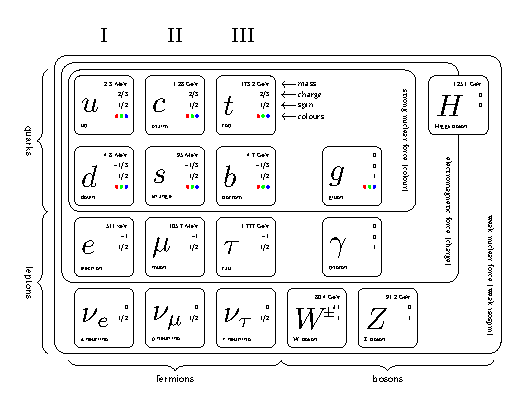
\includegraphics[width=0.99\textwidth]{Figures/SM_diagram.pdf}
\caption{Diagram of the fundamental particles that constitute the SM. Also displayed are the fermion generation shown in Roman numerals, the particles measured mass, charge, spin and colours available for the strong interaction. The particle masses used are taken from Reference~\cite{ParticleDataGroup:2022pth}. The neutrino masses are left blank as the values are unknown. This figure is taken and adjusted from Reference~\cite{sm_diagram}.}
\label{fig:sm_diagram}
\end{figure}

The \ac{SM} is a renormalisable quantum field theory that is built on the principle of local gauge invariance.
The SU(3)$_{\text{C}}$ $\otimes$ SU(2)$_{\text{L}}$ $\otimes$ U(1)$_{\text{Y}}$ is the gauge symmetry group of the \ac{SM}.
This means that the Lagrangian, which governs the interaction of particles, is invariant under such a transformation. 
SU(2)$_{\text{L}}$ $\otimes$ U(1)$_{\text{Y}}$ is the symmetry of the electroweak unification and SU(3)$_{\text{C}}$ is the symmetry of the theory for strong force, named \ac{QCD}. \\

The quantum number associated with the \ac{QCD} SU(3)$_\text{C}$ symmetry is the colour charge C.
Quarks and gluons carry a colour charge and so interact with the strong force.
One characteristic feature of \ac{QCD} is confinement, which requires neutral colour charges and so quarks must be observed in a bound state, named \say{hadrons}.
Another key property is asymptotic freedom, which weakens the interaction strength at higher energy or very short distances \cite{Gross:1973id,Politzer:1973fx}. \\

Electroweak unification was initially proposed by Glashow~\cite{Glashow:1961tr}, Weinberg~\cite{Weinberg:1967tq} and Salam~\cite{Salam:1968rm} to combine the theories of the weak and electromagnetic forces into one.
It is built on the premise of the Dirac equation.
The Dirac Lagrangian for a massless spinor field, $\psi$, is defined as,

\begin{equation}
\mathcal{L}_{\text{Dirac}} = i\bar{\psi}\gamma^{\mu} \partial_{\mu} \psi,
\end{equation}

where $\gamma^{\mu}$ are the gamma matrices and $\partial_{\mu}$ are partial derivatives.
The SU(2)$_{\text{L}}$ transformation operates on the weak isospin, $I$, only for the left-handed spinors and the U(1)$_{\text{Y}}$ transformation operates on the weak hypercharge, $Y=2(Q-I_{3})$, where Q is the charge of the fundamental particles and $I_3$ is the third component of the weak isospin.
The reason for the distinction of the SU(2) symmetry to act only on left-handed spinors is from the observed chirality of fermions under the weak interaction~\cite{Lee:1956qn}.
By invoking gauge invariance of the Dirac Lagrangian, four associated gauge fields are present, $\boldsymbol{W}_{\mu} = (W^{1}_{\mu}, W^{2}_{\mu}, W^{3}_{\mu})$ and $B_{\mu}$.
The Lagrangian then takes the form,

\begin{align}
\begin{split}
\mathcal{L}_{\text{Electroweak}} &= \bar{\psi}_{L}\Big(\partial_{\mu} + \frac{i}{2} g \boldsymbol{W}_{\mu} \cdot \boldsymbol{\sigma} + g^{\prime} Y B_{\mu}  \Big) \psi_L \\
&+ \bar{\psi}_{R}\Big(\partial_{\mu} + + g^{\prime} Y B_{\mu}  \Big) \psi_R - \frac{1}{4} \boldsymbol{W}_{\mu\nu} \cdot \boldsymbol{W}^{\mu\nu} - \frac{1}{4}B_{\mu\nu}B^{\mu\nu},
\end{split}
\end{align}

where $g$ and $g^{\prime}$ are the coupling constants for the SU(2) and U(1) symmetries respectively, the partial derivatives have been replaced with the covariant derivative and the added field tensors $\boldsymbol{W}_{\mu\nu}$ and $B_{\mu\nu}$ are defined as,

\begin{equation}
\boldsymbol{W}_{\mu\nu} = \partial_{\mu} \boldsymbol{W}_{\nu} - \partial_{\nu} \boldsymbol{W}_{\mu} - ig[\boldsymbol{W}_{\mu},\boldsymbol{W}_{\nu}],
\end{equation}

\begin{equation}
B_{\mu\nu} = \partial_{\mu} B_{\nu} - \partial_{\mu} B_{\mu}.
\end{equation}

These fields can be rotated into the physical fields for the photon, Z and W boson with the following transformations,

\begin{align}
\begin{split}
W^{\pm}_{\mu} &= \frac{1}{\sqrt{2}}(W^{1}_{\mu} \mp W^{2}_{\mu}), \\
Z_{\mu} &= W^{3}_{\mu} \cos\theta_{w} - B_{\mu} \sin\theta_w, \\
A_{\mu} &= W^{3}_{\mu} \sin\theta_{w} - B_{\mu} \cos\theta_w,
\end{split}
\label{eqn:rotations}
\end{align}

where $\theta_w$ represents the weak mixing angle and is defined such that

\begin{equation}
\sin\theta_w = \frac{g^{\prime}}{\sqrt{g^2 + g^{\prime 2}}}, \hspace{1cm} \cos\theta_w = \frac{g}{\sqrt{g^2 + g^{\prime 2}}}.
\end{equation}

The W and Z bosons were discovered by the UA1 and UA2 collaborations in 1983~\cite{UA1:1983crd,UA2:1983tsx}, which confirmed the predictions made by electroweak unification.
However, the W and Z bosons were measured to have a non-zero mass and Lagrangian mass terms of the form $\frac{1}{2}m_{Z}^2 Z_{\mu} Z^{\mu}$ or $m_{W}^2 W_{\mu}^{-}W^{+\mu}$ cannot be included as they are not invariant under the SU(2)$_{\text{L}}$ $\otimes$ U(1)$_{\text{Y}}$ gauge symmetry.
The same issue also exists in massive fermions, as the fermion mass term's left- and right-handed chiral states, $m\bar{\psi}\psi = m(\bar{\psi}_R \psi_L + \bar{\psi}_L \psi_R)$,  transform differently and therefore do not remain invariant under the gauge transformation.
To resolve this, the \ac{BEH} mechanism for spontaneous symmetry breaking was theorised.

\subsection{Higgs sector}

The \ac{BEH} mechanism was proposed in the 1960s by Englert and Brout~\cite{Englert:1964et}, Higgs~\cite{Higgs:1964ia,Higgs:1964pj,Higgs:1966ev} and Guralnik, Hagen and Kibble~\cite{Guralnik:1964eu,Kibble:1967sv}.
It works on the principles of spontaneous symmetry breaking of the SU(2)$_{\text{L}}$ $\otimes$ U(1)$_{\text{Y}}$ gauge symmetry.
It does this by introducing a gauge invariant field that has a non-zero \ac{VEV}.
The formalism of this is shown below, starting from a complex scalar doublet $\Phi$, 

\begin{equation}
	\Phi = 
	\begin{pmatrix} 
		\phi^{+} \\
		\phi^{0} \\
	\end{pmatrix},
\end{equation}

where $\phi^{+}$ and $\phi^{0}$ are complex functions.
The Lagrangian and the potential, chosen to fulfil the conditions stated above then takes the form,

\begin{equation}
	\mathcal{L}_{\text{Complex Scalar}} = (\partial_{\mu}\Phi)^{\dagger} (\partial^{\mu}\Phi) - V(\Phi),
\end{equation}

with,

\begin{equation}
V(\phi) = \mu^2 \Phi^{\dagger} \Phi + \lambda (\Phi^{\dagger} \Phi)^2,
\end{equation}

where $\mu^2$ and $\lambda$ are two real parameters. 
$\lambda$ is required to be positive for the vacuum to be stable.
If $\mu^2$ is negative, $\Phi$ will have a non-zero \ac{VEV} and the field will be able to spontaneously break the gauge symmetry.
In the vacuum state, the field must satisfy the criteria,

\begin{equation}
\Phi^{\dagger} \Phi = -\frac{\mu^2}{2\lambda}.
\end{equation}

This potential fulfils the criteria of a non-zero \ac{VEV} as $\Phi$ must be non-zero. 
Choosing a gauge to remove the massless scalar bosons, predicted by Goldstone's theorem~\cite{Goldstone:1961eq}, by taking $\phi^+$ to be zero and $\phi$ to be real.
The ground state of $\Phi$ is found as,

\begin{equation}
\braket{0|\Phi|0} = \frac{1}{\sqrt{2}}
	\begin{pmatrix} 
		0 \\
		\nu \\
	\end{pmatrix},
\end{equation}

where $\nu^2 = \mu^2 / \lambda$ and $\nu$ is the non-zero \ac{VEV}.
The complex doublet can then be written as an expansion around the minimum of the potential,

\begin{equation}
\Phi = \frac{1}{\sqrt{2}}
	\begin{pmatrix} 
		0 \\
		\nu + h(x)\\
	\end{pmatrix}
\end{equation}

Applying the covariant derivative for the electroweak gauge symmetry to produce the Lagrangian for the field, $\Phi$, yields

\begin{align}
\begin{split}
\mathcal{L}_{\text{Higgs}} &= \frac{1}{2}(\partial_{\mu}h)(\partial^{\mu}h) + \frac{1}{8} g^{2} (W_{\mu}^{1} + i W_{\mu}^{2})(W^{1\mu} - i W^{2\mu})(\nu + h)^2 \\
&+ \frac{1}{8} (g W_{\mu}^{3} - g' B_{\mu})(g W^{3\mu} - g' B^{\mu})(\nu + h)^2  \\
&+ \mu^2 (\nu + \Ph)^2 + \lambda (\nu + h)^4.
\end{split}
\end{align}

Mass terms for $W_{\mu}^{1}$ and $W_{\mu}^{2}$ are now present and hence the mass of the W boson is $m_W = \frac{1}{2}g\nu$.
Once again, the remaining states need to be rotated to give the photon and the Z boson fields.
Setting up the non-diagonal mass matrix for the fields $W_{\mu}^{3}$ and $B_{\mu}$, and calculating the eigenvalues to find the diagonal basis, masses of two fields are found, one equal to 0 and the other equal to $\frac{1}{2} \nu \sqrt{g^2 + g^{\prime 2}}$ which represent the photon and Z boson mass respectively.
The transformation to the photon and Z fields as parametrised in Equation~\ref{eqn:rotations} utilises,

\begin{equation}
\tan\theta_W = \frac{g^{\prime}}{g}.
\end{equation}

A mass term for the Higgs boson also arises from the potential of the \ac{BEH} mechanism with $m_{\Ph} = \sqrt{-2\mu^2}$. 
The same mechanism can also be used to add mass terms for quarks and charged leptons.
Gauge invariant couplings to the Higgs bosons and fermion mass terms can be generated from the \ac{BEH} mechanism applied to a Lagrangian term of the form,

\begin{equation}
\mathcal{L}_{\text{Yukawa}} = \lambda_f (\bar{\psi}_{L}\Phi\psi_{R} + \bar{\psi}_{R}\Phi\psi_{L}).
\end{equation}

Upon spontaneous symmetry breaking, $\lambda_{f}$ becomes proportional to the mass of the fermion, and hence the couplings are stronger between heavier fermions and the Higgs field.

\section{Extended Higgs sector}

There is no theoretical limitation to having only one Higgs doublet in the theory.
Therefore, a natural extension to the \ac{SM} Higgs sector is a \ac{2HDM}.
The Lagrangian for such a theory is shown below.

\begin{equation}
\mathcal{L}_{\text{2HDM}} = (D_\mu \Phi_1)^{\dagger} (D_\mu \Phi_1) + (D_\mu \Phi_2)^{\dagger} (D_\mu \Phi_2) - V_{\text{2HDM}}(\Phi_1 ,\Phi_2)
\end{equation}

where,

\begin{align}
\label{eqn:lag_2hdm}
\begin{split}
V_{\text{2HDM}} &= m_{11}^{2}|\Phi_{1}|^2 + m_{22}^{2}|\Phi_{2}|^2 + (m_{12}^{2}\Phi_{1}^{\dagger}\Phi_{2} + \text{h.c.}) \\
&+ \frac{\lambda_1}{2}|\Phi_{1}|^4 + \frac{\lambda_2}{2}|\Phi_{2}|^4 + \lambda_3 |\Phi_{1}|^2 |\Phi_{2}|^2 + \lambda_4  |\Phi_{1}^{\dagger} \Phi_{2}| \\
&+ \frac{1}{2}\Big[ \lambda_5 (\Phi_{1}^{\dagger} \Phi_{2})^{2} + \lambda_6 |\Phi_{1}|^{2} \Phi_{1}^{\dagger} \Phi_{2} +  \lambda_7 |\Phi_{2}|^{2} \Phi_{1}^{\dagger} \Phi_{2} + \text{h.c.} \Big],
\end{split}
\end{align}

where $m_{ij}$ represents the terms in the mass matrix and $\lambda_i$ parametrises the self-couplings of the Higgs sector. 
After the \ac{BEH} mechanism is applied, \ac{2HDM}s predict 5 Higgs bosons; 1 lighter and 1 heavier \ac{CP}-even (\Ph and \PH), 1 \ac{CP}-odd (\PA) and 2 charged (\PHc) particles.
The Lagrangian for the Yukawa interactions with the Higgs bosons in such a theory are,

\begin{equation}
\begin{aligned}
\mathcal{L}^{\text{2HDM}}_{\text{Yukawa}} &= - \sum_{f=u,d,l}\Big(\frac{m_{f}}{\nu}g^{f}_{h}\bar{f}fh + \frac{m_{f}}{\nu}g^{f}_{H}\bar{f}fH -i\frac{m_{f}}{\nu}g^{f}_{A}\bar{f}\gamma_{5}fA\Big)  \\ 
&- \Big[\frac{\sqrt{2}V_{ud}}{\nu}\bar{u}(m_{u}g^{u}_{A}P_{L} + m_{d}g^{d}_{A}P_{R})dH^{+} + \frac{\sqrt{2}m_{l}g^{d}_{A}}{\nu}\bar{\nu}_{L}l_{R}H^{+} + h.c.\Big],
\end{aligned}
\end{equation}

where $u$, $d$, $l$ and $\nu$ represent up-like quark, down-like quark, charged lepton and neutrino fields, the subscript $L$ and $R$ are the left- and right-handed projections performed via the projection operators, $P_L$ and $P_R$ respectively.
$m_{f}$ are the fermion masses, $\nu$ is the vacuum expectation value of the \ac{SM} Higgs doublet, and $g$ are the couplings (relative to the \ac{SM} Higgs boson's couplings) of fermion fields to Higgs fields, $h$, $H$, $A$ and $H^{+}$.
There are four main types of \ac{2HDM}s, which are defined based on which Higgs doublet couples to which group of fermions, named type I, II, X (lepton-specific) and Y (flipped).
The couplings of the fermion groups to the Higgs doublets are shown in Table~\ref{tab:2hdm_doublets}. 
By convention, $\Phi_2$ is chosen to couple to up-like quarks.

\begin{table}[H]
    \centering
    \begin{tabular}{|x{1.0cm}|x{2.0cm}x{2.0cm}x{2.0cm}x{2.0cm}|}
    		\hline
    	 	& Type I & Type II & Type X & Type Y \\
    	 	\hline
    	 	\hline
    	 	$u$ & $\Phi_2$ & $\Phi_2$  & $\Phi_2$  & $\Phi_2$  \\ 
    	 	$d$ & $\Phi_2$ & $\Phi_1$ & $\Phi_2$ & $\Phi_1$ \\
    	 	$l$ & $\Phi_2$ & $\Phi_1$   & $\Phi_1$    & $\Phi_2$ \\
        \hline
    \end{tabular}
    \caption{Table showing which fermion groups couple to which Higgs doublet, in different types of 2HDMs.}
    \label{tab:2hdm_doublets}
\end{table}

The type of \ac{2HDM} determines the formulae for the couplings, $g$, that are functions on two parameters: the \ac{CP}-even ($\alpha$) and \ac{CP}-odd ($\beta$) mixing angles of the mass matrices.
These relative couplings are shown in Table~\ref{tab:2hdm_couplings}.

\begin{table}[H]
    \centering
    \begin{tabular}{|x{1.0cm}|x{2.0cm}x{2.0cm}x{2.0cm}x{2.0cm}|}
    		\hline
    	 	& Type I & Type II & Type X & Type Y \\
    	 	\hline
    	 	\hline
    	 	$g_{h}^{u}$ & $c_{\alpha}/s_{\beta}$ & $c_{\alpha}/s_{\beta}$  & $c_{\alpha}/s_{\beta}$  & $c_{\alpha}/s_{\beta}$  \\ 
    	 	$g_{h}^{d}$ & $c_{\alpha}/s_{\beta}$ & $-s_{\alpha}/c_{\beta}$ & $c_{\alpha}/s_{\beta}$  & $-s_{\alpha}/c_{\beta}$ \\
    	 	$g_{h}^{l}$ & $c_{\alpha}/s_{\beta}$ & $-s_{\alpha}/c_{\beta}$ & $-s_{\alpha}/c_{\beta}$ & $c_{\alpha}/s_{\beta}$  \\
    	 	\hline
    	 	$g_{H}^{u}$ & $s_{\alpha}/s_{\beta}$ & $s_{\alpha}/s_{\beta}$ & $s_{\alpha}/s_{\beta}$ & $s_{\alpha}/s_{\beta}$ \\
    	 	$g_{H}^{d}$ & $s_{\alpha}/s_{\beta}$ & $c_{\alpha}/c_{\beta}$ & $s_{\alpha}/s_{\beta}$ & $c_{\alpha}/c_{\beta}$ \\
    	 	$g_{H}^{l}$ & $s_{\alpha}/s_{\beta}$ & $c_{\alpha}/c_{\beta}$ & $c_{\alpha}/c_{\beta}$ & $s_{\alpha}/s_{\beta}$ \\
    	 	\hline
    	 	$g_{A}^{u}$ & $1/t_{\beta}$ & $1/t_{\beta}$ & $1/t_{\beta}$  & $1/t_{\beta}$ \\
    	 	$g_{A}^{d}$ & $1/t_{\beta}$ & $t_{\beta}$   & $-1/t_{\beta}$ & $t_{\beta}$ \\
    	 	$g_{A}^{l}$ & $1/t_{\beta}$ & $t_{\beta}$   & $t_{\beta}$    & $-1/t_{\beta}$ \\
        \hline
    \end{tabular}
    \caption{Table showing the couplings of fermion groups to additional neutral Higgs bosons in different types of 2HDMs. These are dependent on the mixing angles $\alpha$ and $\beta$. $t_{x}$, $s_{x}$ and $c_{x}$ represent $\tan x$, $\sin x$ and $\cos x$ respectively.}
    \label{tab:2hdm_couplings}
\end{table}

To match the observed Higgs boson measurements to a \ac{CP}-even boson predicted by a \ac{2HDM}, a linear combination of these two states are taken,

\begin{equation}
h_{\text{obs}} = \sin(\beta-\alpha) h + \cos(\beta-\alpha) H.
\end{equation}

Assuming a non-degeneracy of the observed Higgs boson mass, two possible alignment limits are acquired: the normal scenario where $\Ph_{\text{obs}}=\Ph$ and $\cos(\beta-\alpha)=0$ and the inverted scenario where $\Ph_{\text{obs}}=\PH$ and $\sin(\beta-\alpha)=0$.
In the normal scenario the values of the coupling ratios from Table~\ref{tab:2hdm_couplings} are $\cos\alpha/\sin\beta=1$, $\sin\alpha/\cos\beta=-1$, $\sin\alpha/\sin\beta=-1/\tan\beta$ and $\cos\alpha/\cos\beta=\tan\beta$. 
Whilst in the inverted scenario the ratios become $\cos\alpha/\sin\beta=1/\tan\beta$, $\sin\alpha/\cos\beta=\tan\beta$, $\sin\alpha/\sin\beta=1$ and $\cos\alpha/\cos\beta=1$. \\

In the \say{physical basis}, the \ac{2HDM} depends on the following parameters,

\begin{equation}
m_{\Ph}, m_{\PH}, m_{\PA}, m_{\PHc}, \tan\beta, \cos(\beta-\alpha), m_{12}^{2}, \lambda_{6}, \lambda_{7}
\end{equation}

It is common to apply a $\mathbb{Z}_2$ symmetry to a \ac{2HDM} to avoid quadratic divergences and suppress flavour-changing neutral currents~\cite{PhysRevD.15.1958,Ginzburg:2004vp}.
In this case, the basis of parameters is shrunk, as $\lambda_6 = \lambda_7 = 0$.
$\tan\beta$ also represents the ratio of the background expectation values of the two Higgs doublets, $\Phi_2$ and $\Phi_1$.
This is generally taken to be greater than 1 because if less than 1 this leads to weaker couplings with down-type fermions, contradicting the observed fermion mass hierarchy. 
Additionally, taking $\tan\beta < 1$, can result in violations of perturbativity, unitarity and potential vacuum instability in the electroweak sector~\cite{SUSY_Primer}.


\section{Theoretical problems and potential solutions}

\subsection{Hierarchy problem}

The current best measurement for the \ac{SM} Higgs boson’s mass from the \ac{CMS} experiment is 125.38 $\pm$ 0.14 GeV~\cite{CMS:2020xrn} in natural units, which are used throughout this thesis.
The lightness is a concern when considering \say{naturalness} and \ac{BSM} physics. 
The Higgs boson has loop corrections to calculations of its mass. 
Known heavy fermions already provide significant contributions (orders of magnitude greater than the observed mass) to the Higgs boson’s calculated mass. 
On top of this, treating the \ac{SM} as an effective field theory, new physics would be expected in the unexplored regions between the weak scale and the Planck scale
If a new fermion were to be found, $f$, or a heavy scalar, $S$, in such a range, the Higgs boson would be subject to even greater changes in its predicted mass. 
The Feynman diagrams for the mass corrections for a fermion and a scalar are shown in Figure~\ref{fig:Higgs_One_Loop_Corrections}.

\begin{figure}[H]
\centering
    \begin{subfigure}[b]{0.4\textwidth}
    \centering
    \scalebox{0.8}{
    \begin{tikzpicture}
    \begin{feynman}
    \vertex (a) {\(h\)};
    \vertex [right = 1.5cm of a] (b);
    \vertex [right = 1cm of b] (dummy);
    \vertex [right = 1cm of dummy] (c);
    \vertex [above = 1cm of dummy] (e);
    \vertex [below = 1cm of dummy] (f);
    \vertex [right = 1.5cm of c] (d) {\(h\)};
    \diagram* {
    (a) -- [scalar] (b),
    (b) -- [out=90, in=180] (e),
    (e) -- [out=0, in=90, edge label=\(f\)] (c),
    (b) -- [out=-90, in=180] (f),
    (f) -- [out=0, in=-90] (c),
    (c) -- [scalar] (d)
    };
    \end{feynman}
    \end{tikzpicture}
    }
    \caption{}
    \label{fig:corr_fermion}
    \end{subfigure}
    \begin{subfigure}[b]{0.4\textwidth}
    \centering
    \scalebox{0.8}{
    \begin{tikzpicture}
    \begin{feynman}
    \vertex (a) {\(h\)};
    \vertex [right = 2cm of a] (b);
    \vertex [right = 2cm of b] (c) {\(h\)};
    \vertex [above = 1cm of b] (dummy);
    \vertex [left = 1cm of dummy] (d);
    \vertex [above = 1cm of dummy] (e);
    \vertex [right = 1cm of dummy] (f);
    \diagram* {
    (a) -- [scalar] (b),
    (b) -- [scalar, out=180, in=-90] (d),
    (d) -- [scalar, out=90, in=-180] (e),
    (e) -- [scalar, out=0, in=90, edge label=S] (f),
    (f) -- [scalar, out=-90, in=0] (b),
    (b) -- [scalar] (c)
    };
    \end{feynman}
    \end{tikzpicture}
    }
    \caption{}
    \label{fig:corr_scalar}
    \end{subfigure}
    \caption{One-loop corrections to the Higgs boson's mass by a fermion $f$ (a) and a scalar $S$ (b).}
    \label{fig:Higgs_One_Loop_Corrections}
\end{figure}

Figure~\ref{fig:corr_fermion} shows a representation of the fermionic correction to the Higgs boson's mass. 
The Lagrangian term for the coupling of the Higgs field to fermions is $-\lambda_f h \bar{f} f$. 
Hence, it can be determined that the correction to the mass is,

\begin{equation}
\Delta m_{\text{h}}^{2} =  -\frac{\lambda_f}{16\pi^2}\Big[\Lambda_{UV}^{2} -2m_{f}^{2} \ln\Big(\frac{\Lambda_{UV}}{m_f}\Big) \Big] + ... ,
\label{eqn:dm_f}
\end{equation}

where \(\Lambda_{UV}\) is the ultraviolet momentum cut off \cite{SUSY_Primer}.
Beyond this, our effective field theory would be expected to break down and for new physics to be found. \\

Figure~\ref{fig:corr_scalar} illustrates a correction to the Higgs boson's mass by a scalar particle. 
The coupling of a scalar to the Higgs field is represented by the Lagrangian term $-\lambda_S |h|^2 |S|^2$. 
The Higgs boson's mass correction for such a term is derived to be,

\begin{equation}
    \Delta m_{\text{h}}^{2} =  \frac{\lambda_{S}^{2}}{16\pi^2}\Big[\Lambda_{UV}^{2} -2m_{S}^{2} \ln\Big(\frac{\Lambda_{UV}}{m_S}\Big) \Big] + ... .
    \label{eqn:dm_S}
\end{equation}

Equations~\ref{eqn:dm_f} and \ref{eqn:dm_S} show that if the mass of the scalar is equivalent to that of the fermion and $\lambda_f = \lambda_{S}^{2}$, then the Higgs boson's mass corrections cancel. 
This offers a solution to the hierarchy problem, by introducing a new symmetry that extends the \ac{SM}. 
The symmetry relates fermions and bosons and is known as \ac{SUSY}. 
It states that fermions and bosons exist in groups called supermultiplets. 
Each supermultiplet contains fermion and boson states, which are superpartners of one another. 
On-shell each supermultiplet must have an equivalent number of fermionic and bosonic degrees of freedom. 
For this to also hold off-shell, an auxiliary field is added to balance the number of degrees of freedom. \\

If \ac{SUSY} is an unbroken theory, then it would be expected for the superpartners to have the same mass as the \ac{SM} particles. 
This has not been seen experimentally, therefore, \ac{SUSY} must be a broken theory in the vacuum state. 
Soft \ac{SUSY} breaking can be introduced through the addition of a \ac{SUSY} violating Lagrangian term $\mathcal{L}_{\text{soft}}$ where,

\begin{equation}
    \mathcal{L} = \mathcal{L}_{\text{SUSY}} + \mathcal{L}_{\text{soft}}.
\end{equation}

$\mathcal{L}_{\text{soft}}$ contains only mass terms and coupling parameters. 
Defining $m_{\text{soft}}$ as the largest mass scale involved in the soft Lagrangian, $m_{\text{soft}}$ also then defines the mass splitting between the \ac{SM} and supersymmetric particles. 
If the mass splitting becomes significant, the hierarchy problem would be reintroduced as corrections to the Higgs boson's mass would again become large. \\

The \ac{MSSM} is the simplest implementation of \ac{SUSY}.
It introduces sets of new particles named squarks, sleptons, gauginos and Higgsinos as superpartners to quarks, leptons, gauge bosons and the Higgs bosons.
Also added are neutralinos and charginos which are combinations of gauginos and Higgsinos.
Additional contributions to the particle content come from the Higgs sector.
The Higgs sector of the \ac{MSSM} is required to be extended to two Higgs doublets to maintain the gauge symmetries and to cancel quantum mechanical inconsistencies~\cite{SUSY_Primer}.
In particular, a type II \ac{2HDM} is needed to ensure natural Yukawa couplings, minimal flavour violation and tree-level mass relations, that all cannot be achieved with a different extended Higgs sector~\cite{SUSY_Primer}.
At tree level, the \ac{MSSM} Higgs sector is only dependent on $m_{\PA}$ and $\tan\beta$.
At high-order accuracies, benchmark scenarios are needed to set the remaining free parameters.

\section{Experimental tensions and potential solutions}

\subsection{B anomalies}
\label{sec:b_anomalies}

Measurements from the B physics experiments such as LHCb~\cite{LHCb:2021trn,LHCb:2015gmp,LHCb:2017rln,LHCb:2017smo}, BaBar~\cite{Kowalewski:2013mna,BaBar:2013mob} and Belle~\cite{Belle:2015qfa,Belle:2016dyj}, testing lepton flavour conservation, have found deviations away from the \ac{SM} expectation of lepton universality.
The differences are observed in both neutral current ($b\rightarrow s\ell^{+}\ell^{-}$) and charged current ($b\rightarrow c\tau\nu$) transitions.
These B anomalies have prompted the idea for a short-range lepton flavour-violating interaction.
This interaction is theorised to be mediated by a new \say{leptoquark} particle~\cite{Diaz:2017lit,Schmaltz:2018nls}.
In an attempt to fit a model that offers a combined explanation of these results, it was found that a U(1) vector leptoquark was the only leptoquark that could offer a simultaneous explanation of all anomalous results~\cite{Cornella:2021sby}. 
Such a leptoquark would couple to fermions by the Lagrangian shown below.

\begin{equation}
\lag_{U} = \frac{g_{U}}{\sqrt{2}} U^{\mu} \big[ \beta_{L}^{i\alpha}( \bar{q}_{L}^{i} \gamma_{\mu} l_{L}^{\alpha}) + \beta_{R}^{i\alpha}( \bar{d}_{R}^{i} \gamma_{\mu} e_{R}^{\alpha}) \big] + \text{h.c.}
\end{equation}

where $g_{U}$ is the coupling scaling parameter and $\beta_{L}$ and $\beta_{R}$ are the left and right-handed mixing matrices,

\begin{equation}
\beta_{L} = 
\begin{pmatrix}
0 & 0 & 0 \\
0 & \beta_{L}^{s\mu} & \beta_{L}^{s\tau} \\
0 & \beta_{L}^{b\mu} & 1
\end{pmatrix},
\hspace{1cm}
\beta_{R} = 
\begin{pmatrix}
0 & 0 & 0 \\
0 & 0 & 0 \\
0 & 0 & \beta_{R}^{b\tau}
\end{pmatrix}.
\end{equation}

The coupling $g_{U}$ is defined such that $\beta_{L}^{b\tau}=1$, and the negligible matrix elements for the fit are set to 0.
The fit to the B anomalies performed in Reference~\cite{Cornella:2021sby}, found the best-fit values for each left-handed mixing matrix parameter based on two scenarios for $\beta^{b\tau}_{R}$, namely $\beta^{b\tau}_{R} = 0$ and $\beta^{b\tau}_{R} = -1$.
These are named VLQ BM 1 and VLQ BM 2 respectively.
These represent no and maximal right-handed contributions. 
The best fit results to the matrix parameters are shown in Table~\ref{tab:vlq_bestfit}.

\begin{table}[h]
\centering
\begin{tabular}{|c|c||c|c|c|}
\hline
Scenario & $\beta^{b\tau}_{R}$ & $\beta^{b\mu}_{L}$ & $\beta^{s\tau}_{L}$ & $\beta^{s\mu}_{L}$ \\
\hline
\hline
VLQ BM 1 & $0$ & $-0.15^{+0.13}_{-0.11}$ & $0.19^{+0.06}_{-0.09}$ & $0.014^{+0.01}_{-0.01}$ \\
VLQ BM 2 & $-1$ & $-0.14^{+0.12}_{-0.11}$ & $0.19^{+0.05}_{-0.08}$ & $0.03^{+0.01}_{-0.02}$ \\
\hline
\end{tabular}
\caption{Best fit values and uncertainties for mixing matrix parameters as given in Reference~\cite{Cornella:2021sby}.}
\label{tab:vlq_bestfit}
\end{table}

The fit also provides a 1$\sigma$ and 2$\sigma$ bound on allowed values for the ratio of the vector leptoquark mass $m_{U}$, to the coupling constant $g_{U}$, and these are,

\begin{align}
\begin{split}
\text{VLQ BM 1}, \hspace{0.2cm} 1\sigma&: 0.70 < g_{U}/m_{U} \text{ (1/TeV)} < 1.09, \\
\text{VLQ BM 1}, \hspace{0.2cm} 2\sigma&: 0.57 < g_{U}/m_{U} \text{ (1/TeV)} < 1.38, \\
\text{VLQ BM 2}, \hspace{0.2cm} 1\sigma&: 0.49 < g_{U}/m_{U} \text{ (1/TeV)} < 0.67, \\
\text{VLQ BM 2}, \hspace{0.2cm} 2\sigma&: 0.39 < g_{U}/m_{U} \text{ (1/TeV)} < 1.25.
\end{split}
\end{align}

\subsection{Muon g-2 anomaly}
\label{sec:gm2_anomaly}

The measurement of the muon anomalous magnetic moment from the Fermilab National Accelerator Laboratory muon g-2 experiment~\cite{Muong-2:2021ojo}, combined with earlier results from the Brookhaven National Laboratory E821 measurement~\cite{Muong-2:2006rrc}, find the difference of $a_\mu$ between the experiment value and \ac{SM} prediction to be,

\begin{equation}
\Delta a_{\mu}^{\text{obs}} = a_{\mu}^{\text{exp}} - a_{\mu}^{\text{SM}} = (251 \pm 59) \times 10^{-11},
\end{equation}

where $a_{\mu}=(g-2)_{\mu}/2$. 
This is a 4.2 $\sigma$ deviation away from the \ac{SM} expectation.
One potential solution to this deviation is a \ac{2HDM}.
This contributes in two ways to $\Delta a_{\mu}$, which is defined as the difference between the $a_{\mu}$ predicted with the \ac{2HDM} included and using just the \ac{SM}. 
These are one-loop and two-loop Bar-Zee diagrams~\cite{Ilisie:2015tra,Barr:1990vd}, that can be mediated by any of the additional Higgs bosons.
In this context, $\phi$ is used as the \ac{CP}-even additional Higgs boson, h or H, depending on which particle is not matched to the observed Higgs boson. \\

\begin{figure}[h]
  \centering
  \begin{subfigure}[b]{0.4\textwidth}
  \scalebox{1.15}{
  \begin{tikzpicture}
    \begin{feynman}
    \vertex [label=left:$\mu$] (c1) at (0,0);
    \vertex (c2) at (1,0);
    \vertex (c3) at (2,0);
    \vertex (c4) at (3,0);
    \vertex [label=right:$\mu$] (c5) at (4,0);
    \vertex [label=above:$\gamma$](t3) at (2,1);
    \vertex [label=below:$\phi/A$](b3) at (2,-1);
    \diagram* {
    (c1) -- [fermion] (c2),
    (c2) -- [fermion] (c3),
    (c3) -- [fermion] (c4),
    (c4) -- [fermion] (c5),
    (c2) -- [scalar, out=-90, in=180] (b3),
    (b3) -- [scalar, out=0, in=-90] (c4),
    (c3) -- [photon] (t3),
    };
    \end{feynman}
   \end{tikzpicture}
  }
  \caption{}
  \end{subfigure}
   \centering
  \begin{subfigure}[b]{0.4\textwidth}
  \scalebox{1.15}{
  \begin{tikzpicture}
    \begin{feynman}
    \vertex [label=left:$\mu$] (c1) at (0,0);
    \vertex (c2) at (1,0);
    \vertex [label=below:$\nu_{\mu}$] (c3) at (2,0);
    \vertex (c4) at (3,0);
    \vertex [label=right:$\mu$] (c5) at (4,0);
    \vertex (t13) at (2,1.6);
    \vertex [label=above:$\gamma$](t23) at (2,2.6);
    \vertex [label=left:$H^{\pm}$] (l1) at (1.5,0.8);
    \vertex [label=right:$H^{\pm}$] (l1) at (2.5,0.8);
    \diagram* {
    (c1) -- [fermion] (c2),
    (c2) -- [fermion] (c4),
    (c4) -- [fermion] (c5),
    (c2) -- [scalar] (t13),
    (c4) -- [scalar] (t13),
    (t13) -- [photon] (t23),
    };
    \end{feynman}
   \end{tikzpicture}
  }
  \caption{}
  \end{subfigure}
  \caption{Examples of one-loop Bar-Zee Feynman diagrams for the contribution from $\phi$ and A (a) and $H^{\pm}$ (b).}
\end{figure}


\begin{figure}[h]
  \centering
  \begin{subfigure}[b]{0.4\textwidth}
  \scalebox{1.15}{
  \begin{tikzpicture}
    \begin{feynman}
    \vertex [label=left:$\mu$] (b1) at (0,0);
    \vertex (b2) at (1,0);
    \vertex [label=below:$\mu$] (b3) at (2,0);
    \vertex (b4) at (3,0);
    \vertex [label=right:$\mu$] (b5) at (4,0);
    \vertex (bm1) at (1.5,1);
    \vertex (bm2) at (2.5,1);
    \vertex (tm1) at (2,1.87);
    \vertex [label=above:$\gamma$] (t1) at (2,2.87);
    \vertex [label=left:$\phi/A$] (l1) at (1.25,0.5);
    \vertex [label=right:$\gamma$] (l2) at (2.75,0.5);
    \vertex [label=right:$f$] (l3) at (2.5,1.75);
    \diagram* {
    (c1) -- [fermion] (c2),
    (c2) -- [fermion] (c4),
    (c4) -- [fermion] (c5),
    (c2) -- [scalar] (bm1),
    (c4) -- [boson] (bm2),
    (tm1) -- [fermion, out=0, in=60] (bm2),
    (bm2) -- [fermion, out=-120, in=-60] (bm1),
    (bm1) -- [fermion, out=120, in=180] (tm1),
    (tm1) -- [photon] (t1),
    };
    \end{feynman}
   \end{tikzpicture}
  }
  \caption{}
  \end{subfigure}
   \centering
  \begin{subfigure}[b]{0.4\textwidth}
  \scalebox{1.15}{
  \begin{tikzpicture}
    \begin{feynman}
    \vertex [label=left:$\mu$] (b1) at (0,0);
    \vertex (b2) at (1,0);
    \vertex [label=below:$\nu_{\mu}$] (b3) at (2,0);
    \vertex (b4) at (3,0);
    \vertex [label=right:$\mu$] (b5) at (4,0);
    \vertex (bm1) at (1.5,1);
    \vertex (bm2) at (2.5,1);
    \vertex (tm1) at (2,1.87);
    \vertex [label=above:$\gamma$] (t1) at (2,2.87);
    \vertex [label=left:$H^{\pm}$] (l1) at (1.25,0.5);
    \vertex [label=right:$W^{\pm}$] (l2) at (2.75,0.5);
    \vertex [label=right:$t/b$] (l3) at (2.5,1.75);
    \vertex [label=left:$t/b$] (l3) at (1.5,1.75);
    \vertex [label=below:$b/t$] (l3) at (2,0.8);
    \diagram* {
    (c1) -- [fermion] (c2),
    (c2) -- [fermion] (c4),
    (c4) -- [fermion] (c5),
    (c2) -- [scalar] (bm1),
    (c4) -- [photon] (bm2),
    (tm1) -- [fermion, out=0, in=60] (bm2),
    (bm2) -- [fermion, out=-120, in=-60] (bm1),
    (bm1) -- [fermion, out=120, in=180] (tm1),
    (tm1) -- [photon] (t1),
    };
    \end{feynman}
   \end{tikzpicture}
  }
  \caption{}
  \end{subfigure}
  \caption{Examples of two-loop Bar-Zee Feynman diagrams for the contribution from $\phi$ and A (a) and $H^{\pm}$ (b). Note that other fundamental particles can also contribute to the loop.}
\end{figure}

The one-loop contribution to $\Delta a_{\mu}$ is positive from $\phi$ and negative from $A$ and $H^{\pm}$, however, the more significant contribution comes from two-loop Bar-Zee diagrams with heavy fermions in the loop which gives a positive shift to $\Delta a_{\mu}$.
To fulfil the requirements for the anomaly, enhanced couplings between additional Higgs bosons and muons are needed.
This gives two options: a type II or a type X \ac{2HDM}, both at large values of $\tan\beta$.
The type II \ac{2HDM}, which also offers enhanced couplings to down-like quarks, is heavily constrained by \ac{LEP}, Tevatron and \ac{LHC} searches and an available region of phase space to explain the anomaly is not easily found.
However, the type X \ac{2HDM}, with only lepton coupling enhancements at high $\tan\beta$, is relatively unconstrained due to suppressed quark-initiated production modes of additional Higgs bosons. \\

Reference~\cite{Jueid:2021avn} puts an upper limit of $m_{A} \lesssim 200$ GeV, which is required for an explanation of $\Delta a_{\mu}^{\text{obs}}$.
Further constraints are placed on the phase space from theoretical stabilities, electroweak precision measurements and collider bounds.
The final available phase space for a type X \ac{2HDM} in the alignment scenario to explain the muon g-2 anomaly is shown in Table~\ref{tab:gm2region}.

\begin{table}[H]
    \centering
    \begin{tabular}{|p{1.5cm}|x{2.2cm}x{2.2cm}x{2.2cm}x{2.2cm}|}
         \hline
         Scenario & $\tan\beta$ & $m_{A}$ (GeV) & $m_{\phi}$ (GeV) & $m_{H^{\pm}}$ (GeV) \\
         \hline
         \hline
         Normal & $\geq 90$ & [62.5,145] & [130,245] & [95,285] \\
         Inverted & $\geq 120$ & [70,105] & [100,120] & [95,185] \\
         \hline
    \end{tabular}
    \caption{Regions of interest for muon g-2 anomaly in the type X 2HDM in the normal and inverted alignment scenarios as suggested in Reference~\cite{Jueid:2021avn}.}
    \label{tab:gm2region}
\end{table}

%\newpage
%\chapter{The LHC and CMS experiment}
\label{sec:cms}

This chapter will explain the apparatus used to generate and collect the datasets that are utilised for the physics analyses described in Chapters~\ref{sec:bsm_H_to_tau_tau_analysis} and \ref{sec:H_A_to_4_tau_analysis}.
This is split into two parts.
Firstly, there is an overview of the \ac{LHC} and a description of how proton-proton collisions at a centre-of-mass energy ($\sqrt{s}$) of 13 TeV are achieved.
Secondly, an explanation of the \ac{CMS} detector is given, including a look at the individual sub-detectors, that are crucial to the reconstruction of particles originating from the proton-proton collisions.

\section{The LHC}

The \ac{LHC}~\cite{Evans:2008zzb}, located at \ac{CERN} just outside Geneva, is a synchrotron measuring 27 km in circumference, installed in the tunnel previously used by the \ac{LEP} accelerator~\cite{203828}. 
Upon design, its primary purpose was to provide collisions between proton beams, generating centre-of-mass energies of up to 14 TeV and an instantaneous luminosity of approximately $10^{34}$ cm$^{−2}$s$^{−1}$. 
Figure~\ref{fig:CERN_Schematic} illustrates the arrangement of the \ac{LHC} and the \ac{CERN} accelerator complex. 
Protons are supplied to the \ac{LHC} through a sequence of accelerators: Linac4 (Linac2 pre-2020), \ac{PSB}, \ac{PS}, and the \ac{SPS}, that successively raise the energies of the protons to 50 MeV, 1.4 GeV, 25 GeV, and 450 GeV respectively~\cite{Benedikt:2004wm}. 
When the final energy has been achieved, the \ac{SPS} injects bunched protons into the \ac{LHC}'s beam pipes as two counter-rotating beams. 
Each bunch contains over $10^{11}$ protons, with each one separated by 25 ns and each beam consists of 2808 bunches. 
The protons are accelerated to collision energy using eight 400 MHz \ac{RF} cavities and kept in a circular trajectory with 1232 niobium-titanium superconducting dipole magnets. 
These magnets must be maintained at their operating temperature of 1.9 K to generate magnetic fields up to 8.4 T, requiring the use of superfluid helium. 
The bunches are collided at four intersection points surrounded by the ALICE~\cite{ALICE:2008ngc}, ATLAS~\cite{ATLAS:2008xda}, CMS~\cite{CMS_Setup} and LHCb~\cite{LHCb:2008vvz} detectors, at a collision rate of 40 MHz. \\

\begin{figure}[t]
    \centering
    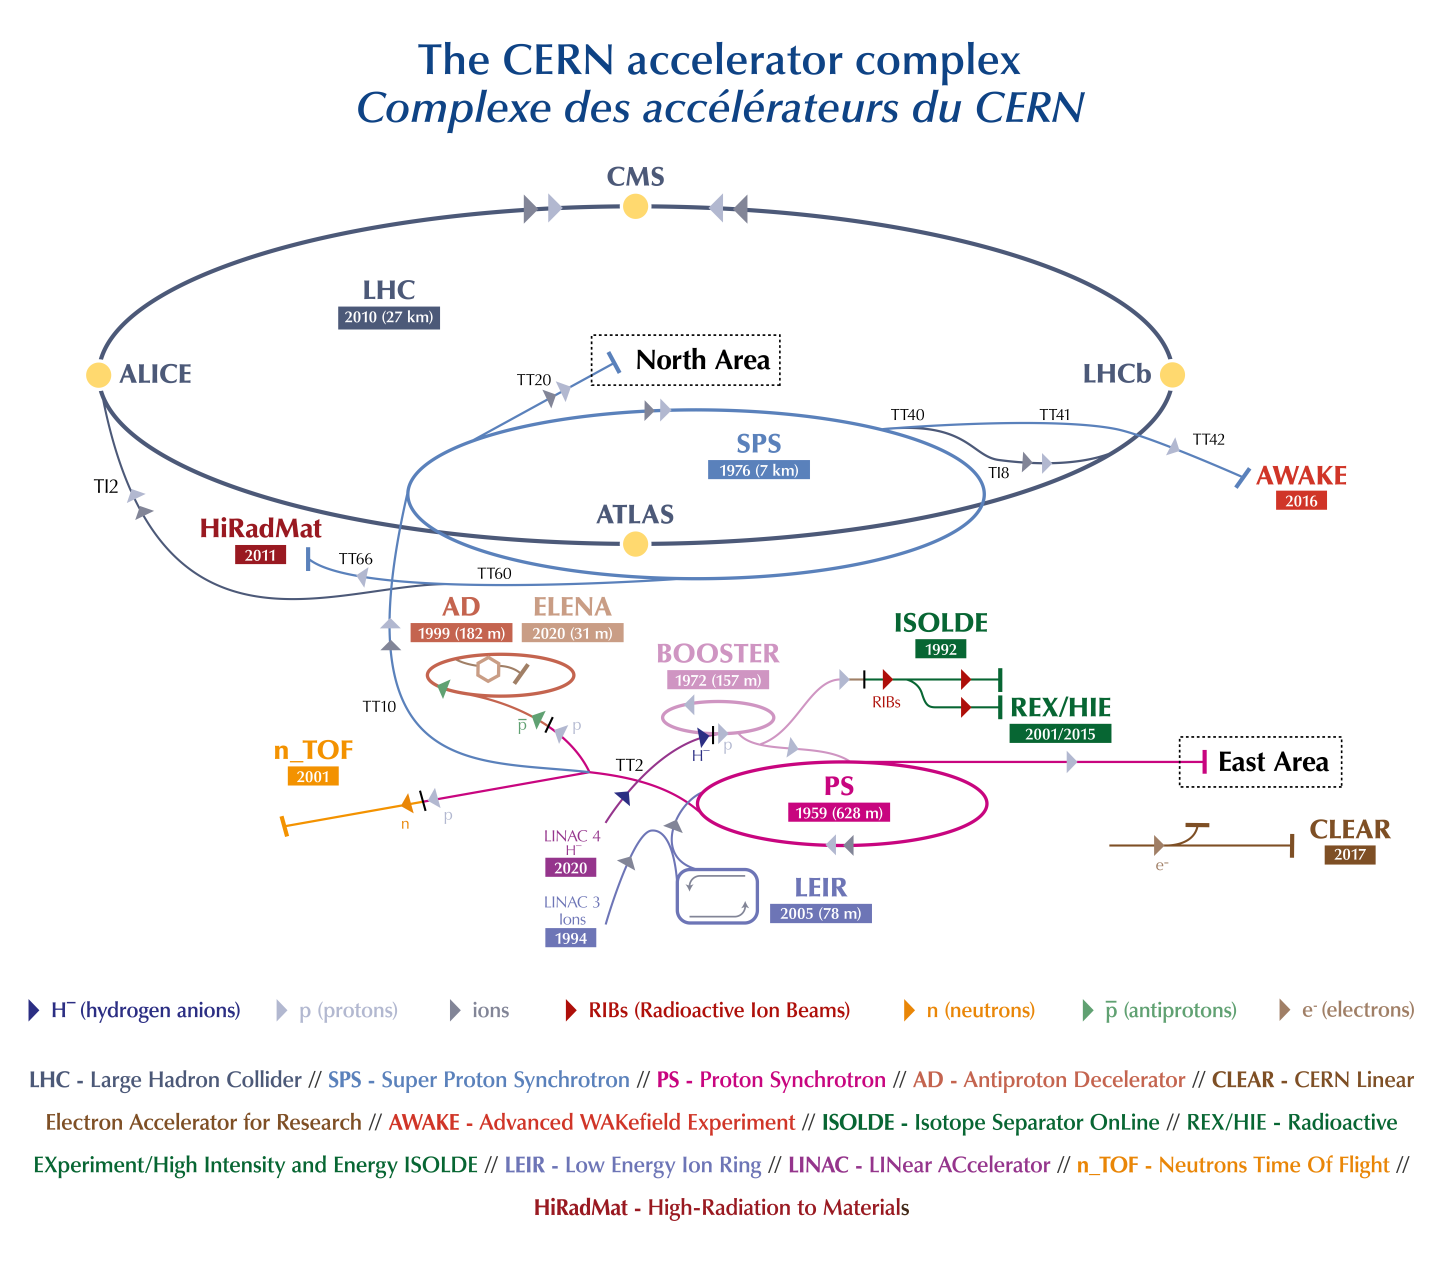
\includegraphics[width=\textwidth]{Figures/cern.png}
    \caption[Diagram of the CERN accelerator complex.]{A schematic diagram of the CERN accelerator complex~\cite{Bartosik:2847538}.}
    \label{fig:CERN_Schematic}
\end{figure}

The rate of events for a process produced in \ac{LHC} collisions can be expressed as,

\begin{equation}
R_{\text{event}} = L_{\text{inst}} \sigma(\sqrt{s}), 
\end{equation}

where $\sigma$ represents the cross-section of the process and is a function of $\sqrt{s}$, and $L_{\text{inst}}$ denotes the \ac{LHC} machine's instantaneous luminosity, that depends only on the beam parameters and can be calculated by,

\begin{equation}
L_{\text{inst}} = \frac{n_{b}N_{b}^{2}f_{\text{rev}}\gamma_{r}}{4\pi \epsilon_{n}\beta^{*}}F,
\end{equation}

where $n_b$ is the number of bunches per beam, $N_b$ is the number of particles per bunch, $f_{\text{rev}}$ is the revolution frequency, $\gamma_r$ is the relativistic gamma factor, $\epsilon_n$ is the normalised transverse beam emittance, $\beta^*$ is the beta function at the collision point, and $F$ is a reduction factor which accounts for the crossing angle of the beams at the collision point. 
One disadvantage of an increase in the instantaneous luminosity is the increase of \ac{PU}, defined as the number of additional inelastic proton-proton collisions per bunch crossing. \\

\begin{figure}[t]
    \centering
    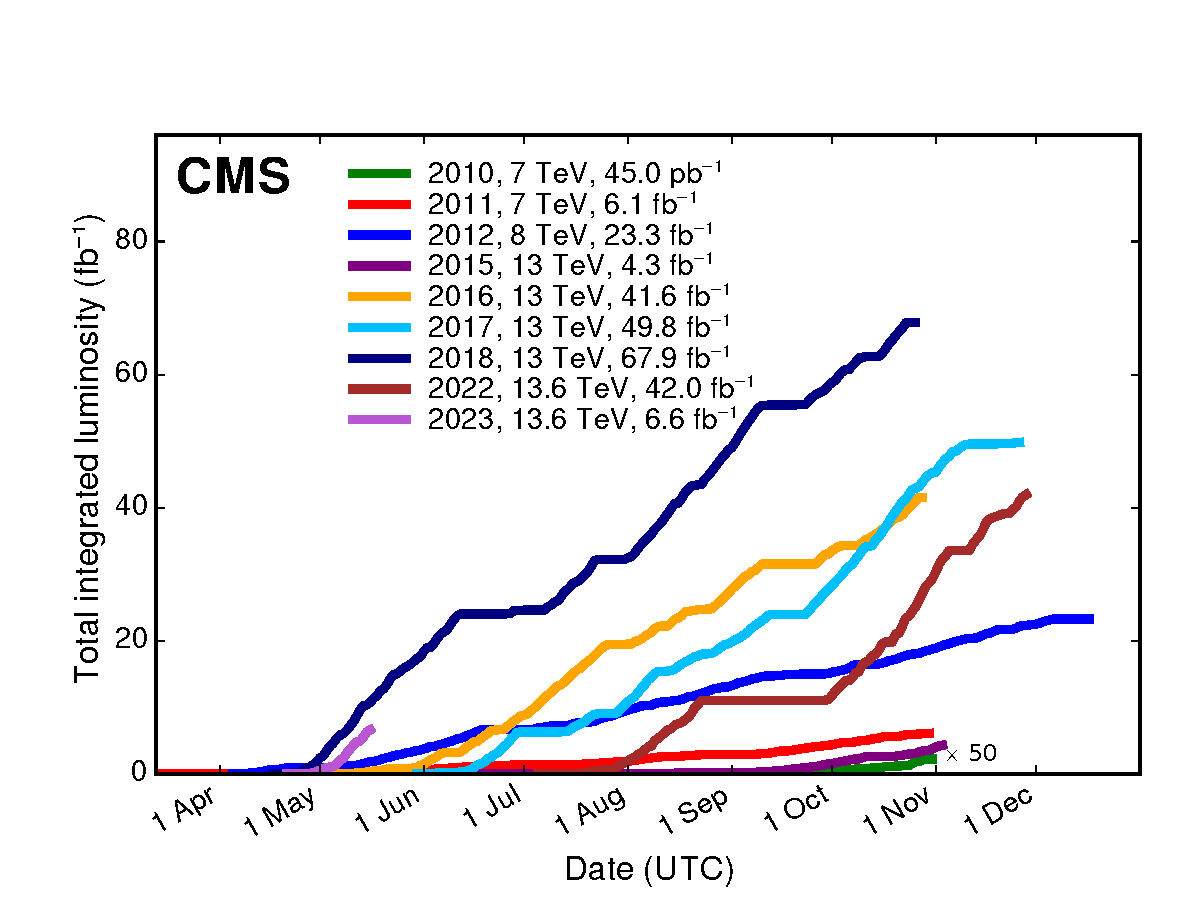
\includegraphics[width=0.9\textwidth]{Figures/int_lumi_cumulative_pp_2.pdf}
    \caption[Plot of the total integrated luminosity collected by the CMS experiment.]{The total integrated luminosity for proton-proton collisions collected by the \ac{CMS} experiment between 2010 and May 2023~\cite{lumi}.}
    \label{fig:int_lumi}
\end{figure}

The \ac{LHC} began its first physics collisions in 2010, initially colliding beams at $\sqrt{s}$ = 7 TeV, which was increased to 8 TeV throughout 2012. 
Following this data-taking period, known as Run 1, the \ac{LHC} underwent a two-year \ac{LS1} to undergo upgrades in preparation for an increase in $\sqrt{s}$. 
In 2015, the \ac{LHC} was restarted, initiating its Run 2 phase of data collection at $\sqrt{s}$ = 13 TeV, which lasted until the end of 2018. 
During Run 2, the \ac{LHC} achieved and surpassed its original design luminosity by obtaining a record peak luminosity of $2.1\times10^{34}$ cm$^{−2}$s$^{−1}$ in 2018.
Subsequently, the \ac{LHC} performed a second update period, the \ac{LS2}, lasting for approximately three years, whereafter the data collection for Run 3 began at $\sqrt{s}$ = 13.6 TeV.
Figure~\ref{fig:int_lumi} illustrates the total integrated luminosity of proton-proton collisions delivered to the \ac{CMS} detector at the time of writing.
The data used for the analyses described in this thesis correspond to the full Run 2 dataset collected during the 2016--2018 data-taking periods at 13 TeV. 
Only data recorded by \ac{CMS}, where all sub-detectors were functioning correctly are certified and are used in physics analyses. 
This equates to 36.3 fb$^{−1}$, 41.5 fb$^{−1}$ and 59.7 fb$^{-1}$ of data collected in 2016, 2017 and 2018 respectively. \\

\section{The CMS detector}

The \ac{CMS} detector was engineered to fulfil the rigorous demands of the \ac{LHC} physics program. 
Its primary objective is to achieve sensitivity to the Higgs boson and novel phenomena at the TeV energy scale. 
Weighing 12,500 tonnes and measuring 21.6 m in length with a diameter of 14.6 m, the \ac{CMS} detector uses an array of sub-detectors encircling the central beam axis~\cite{CMS_Setup}. 
The layout of the \ac{CMS} detector is shown in Figure~\ref{fig:CMS_Schematic}.
A superconducting solenoid, operating at a magnetic field strength of 3.8 T, surrounds the inner tracker, electromagnetic calorimeter, and hadronic calorimeter. 
Situated outside the solenoid within the iron return yoke are gaseous muon detectors, positioned to accurately measure muons. 
The \ac{CMS} detector adopts a coordinate system centred at the collision point, with the $y$-axis oriented vertically, the $x$-axis directed radially inward toward the \ac{LHC} centre, and the $z$-axis aligned with the beam direction. 
The transverse energy ($E_T$) and transverse momentum ($\pT$) are defined in the $x$-$y$ plane. 
The azimuthal angle ($\phi$) and polar angle ($\theta$) are measured relative to the $x$-axis in the $x$-$y$ plane and $z$-axis relative to the $z$-$y$ plane, respectively. 
$r$ is used as the radial distance in the $x$-$y$ plane.
Pseudorapidity ($\eta$), defined as $\eta = -\ln[\tan(\theta/2)]$, is used due to its gauge invariance, and distances between objects in the $\phi$-$\eta$ plane are characterised by the metric $\Delta R = \sqrt{\Delta\phi^2 + \Delta\eta^2}$. 

\begin{figure}[!hbtp]
    \centering
    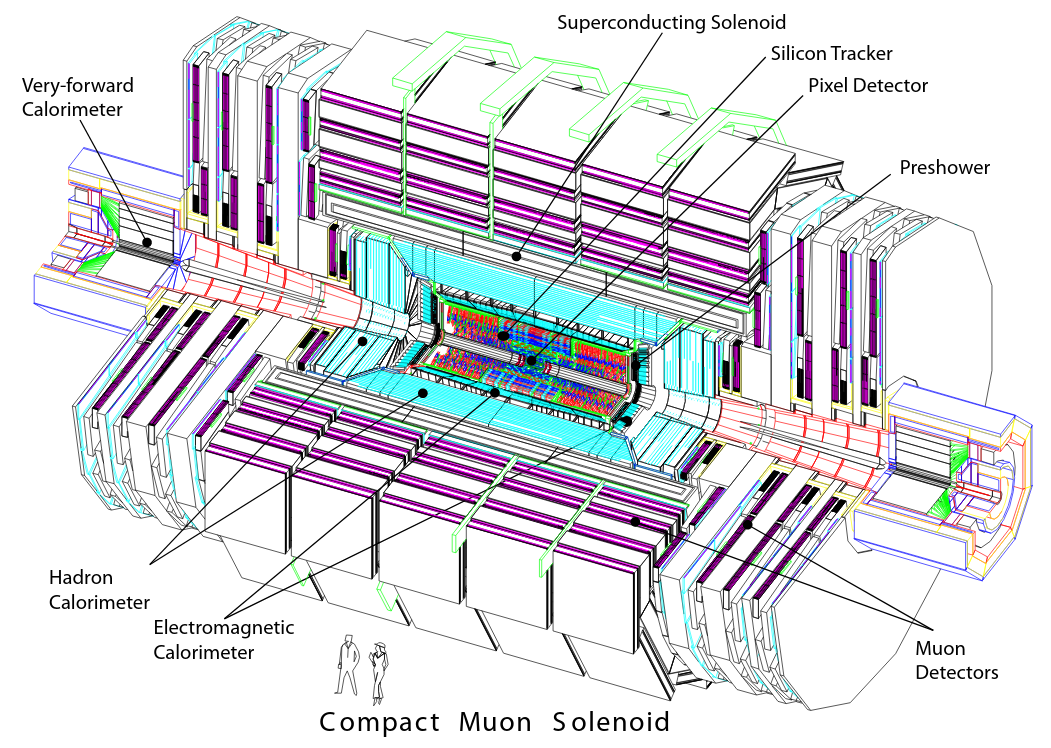
\includegraphics[width=0.9\textwidth]{Figures/CMS_Detector.png}
    \caption[Diagram of the CMS detector.]{A perspective view of the \ac{CMS} detector \cite{CMS_Setup}.}
    \label{fig:CMS_Schematic}
\end{figure}

\subsection{Tracker}

Closest to the interaction point in the \ac{CMS} experiment is the tracker~\cite{CMS_Setup,Malberti:2014pda,CMS:2012sda}, which is essential for precise measurements of charged particle trajectories and the determination of the \ac{PV} and other vertices, as explained in Section~\ref{sec:track_and_vertex}. 
A silicon tracking detector is used to meet the requirements of high granularity and fast response for the large number of particles generated in each bunch crossing, as well as being radiation hard to deal with the particle flux.
The tracker consists of a pixel detector and a silicon strip detector as shown in Figure~\ref{fig:tracker}. \\

\begin{figure}[!hbtp]
    \centering
    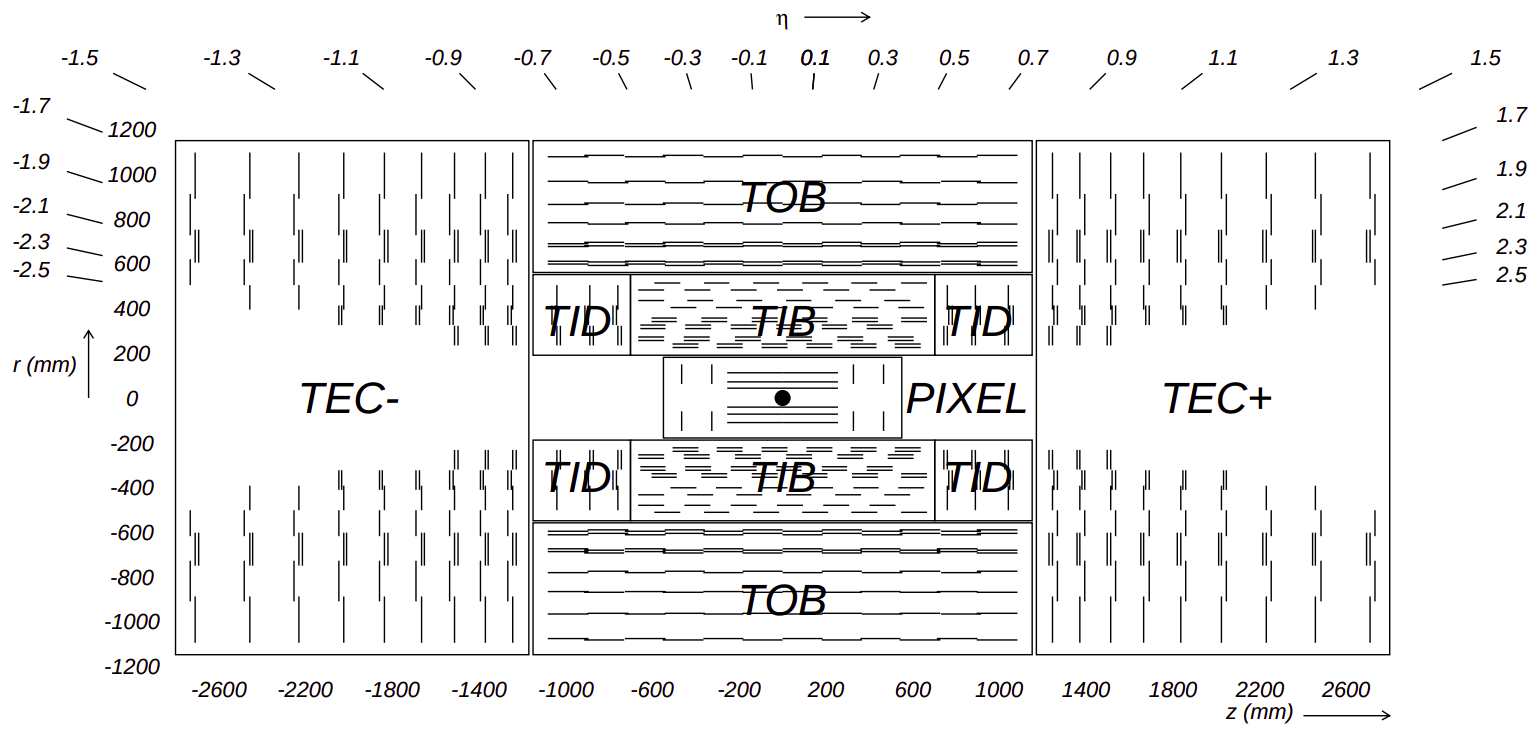
\includegraphics[width=\textwidth]{Figures/tracker.png}
    \caption[Diagram of the CMS tracker.]{Schematic of the CMS tracker (pre-pixel upgrade) in the $r$-$z$ plane, showing the position of the pixel detector as well as the TIB, TID, TOB, and TEC strip detectors. The lines represent detector modules and the double lines represent back-to-back modules~\cite{CMS_Setup}.}
    \label{fig:tracker}
\end{figure}

The pixel detector covers the pseudorapidity range $|\eta| < 2.5$ and is composed of three cylindrical pixel modules and two disk pixel modules. 
It contains 66 million silicon pixels, each with dimensions of $100 \times 150$ $\upmu$m${^2}$. 
This configuration provides a spatial resolution of 15--20 $\upmu$m in both the $r$-$\phi$ plane and the $z$ direction, enabling three-dimensional vertex reconstruction~\cite{CMS_Setup}.
The original tracker was built to handle an instantaneous luminosity of $10^{34}$ cm$^{2}$s$^{-1}$ and an average \ac{PU} of 25.
To cope with higher luminosities and increased event \ac{PU}, the pixel detector was upgraded in 2016/2017 to handle approximately double the instantaneous luminosity and \ac{PU}~\cite{CMS:2012sda}. 
The upgraded detector consists of four barrel module layers and three endcap disks, resulting in 124 million pixels. \\

A silicon strip detector surrounds the pixel detector and is divided into four subsystems: the \ac{TIB}, \ac{TID}, \ac{TOB}, and \ac{TEC}~\cite{CMS_Setup}. 
The \ac{TIB} and \ac{TID} provide four layers of silicon strip detectors in the barrel region and three disks at each end, extending up to a radius of 55 cm. 
The \ac{TOB} consists of six barrel layers extending up to an outer radius of 116 cm, while the \ac{TEC} comprises nine disks covering a range of $|z|$ from 124 cm to 282 cm. 
The silicon strips have various thicknesses and widths, providing multiple measurements of the $r$-$\phi$ position with resolutions ranging from 23-35 $\upmu$m in the \ac{TIB} to 35-53 $\upmu$m in the \ac{TOB}~\cite{CMS_Setup}. \\

In addition to the main components, the tracker includes back-to-back mounted micro-strip detector modules to provide additional measurements of the $z$ coordinate in specific regions. 
The overall tracker layout ensures the presence of at least three hits in the pixel detector (at least four hits for the upgraded detector) and at least nine hits in the silicon-strip tracker, with a minimum of four two-dimensional measurements among them.

\subsection{Electromagnetic calorimeter}

The \ac{CMS} \ac{ECAL} is a hermetic homogeneous calorimeter designed to detect high-energy electrons and photons~\cite{CMS_Setup,CMS:2013lxn}. 
In total, 75,848 lead tungstate (PbWO$_4$) crystals are sorted in a barrel and endcap configuration. 
PbWO$_4$ was chosen as the crystal material because of its radiation hardness, high density, short radiation length, and small Molière radius, enabling the construction of a compact and finely granular \ac{ECAL}. 
Scintillation light produced by showering electrons and photons in the crystals is converted into an electrical signal by photodetectors such as avalanche photodiodes in the barrel and vacuum phototriodes in the endcaps. 
The scintillation decay time of the crystals matches the 25 ns \ac{LHC} bunch crossing time, ensuring that a significant portion of the light is emitted between bunch crossings. \\

The \ac{ECAL} is placed outside of the tracker but within the magnet bore and covers the pseudorapidity range $|\eta| < 3.0$. 
It comprises of an \ac{EB} covering $|\eta| < 1.479$ and an \ac{EE} covering $1.479 < |\eta| < 3.0$. 
A diagram of this is shown in Figure~\ref{fig:ecal}.
The barrel region consists of 61,200 crystals with 360-fold granularity in $\phi$ and 170-fold granularity in $\eta$. 
The crystals are tapered with a front face area of $0.0174 \times 0.0174$ in $\eta$-$\phi$ ($22 \times 22$ mm$^2$) and a length of 230 mm. 
The endcaps house 7,324 crystals arranged in a rectangular $x$-$y$ grid, each with a front face area of $28.62 \times 28.62$ mm$^2$ and a length of 220 mm. \\

The \ac{ECAL} system also includes pre-shower detectors placed in front of each endcap to identify photons from neutral pion decays and improve electron identification and position resolution. 
These detectors consist of lead radiators to initiate showering and silicon-strip sensors to measure the deposited energy. \\

The \ac{ECAL} energy resolution is parametrised as a function of the incident particle energy E, with terms for the stochastic S, noise N, and constant C contributions.

\begin{equation}
\Big(\frac{\sigma}{E}\Big)^2 = \Big(\frac{S}{\sqrt{E}}\Big)^2 + \Big( \frac{N}{E} \Big) + C^2
\end{equation}

The stochastic term captures fluctuations in lateral shower containment and photon yield, the noise term accounts for electronics' noise and \ac{PU}, and the constant term arises from the non-uniformity of the longitudinal response and calibration errors. 
Measurements using electron beams in 2004 found the values of S = 0.028 GeV$^{1/2}$, N = 0.12 GeV, and C = 0.003 for the \ac{ECAL} energy resolution, however, measurements in 2006 found a 10\% improvement in the noise performance.~\cite{CMS_Setup}.

\begin{figure}[!hbtp]
    \centering
    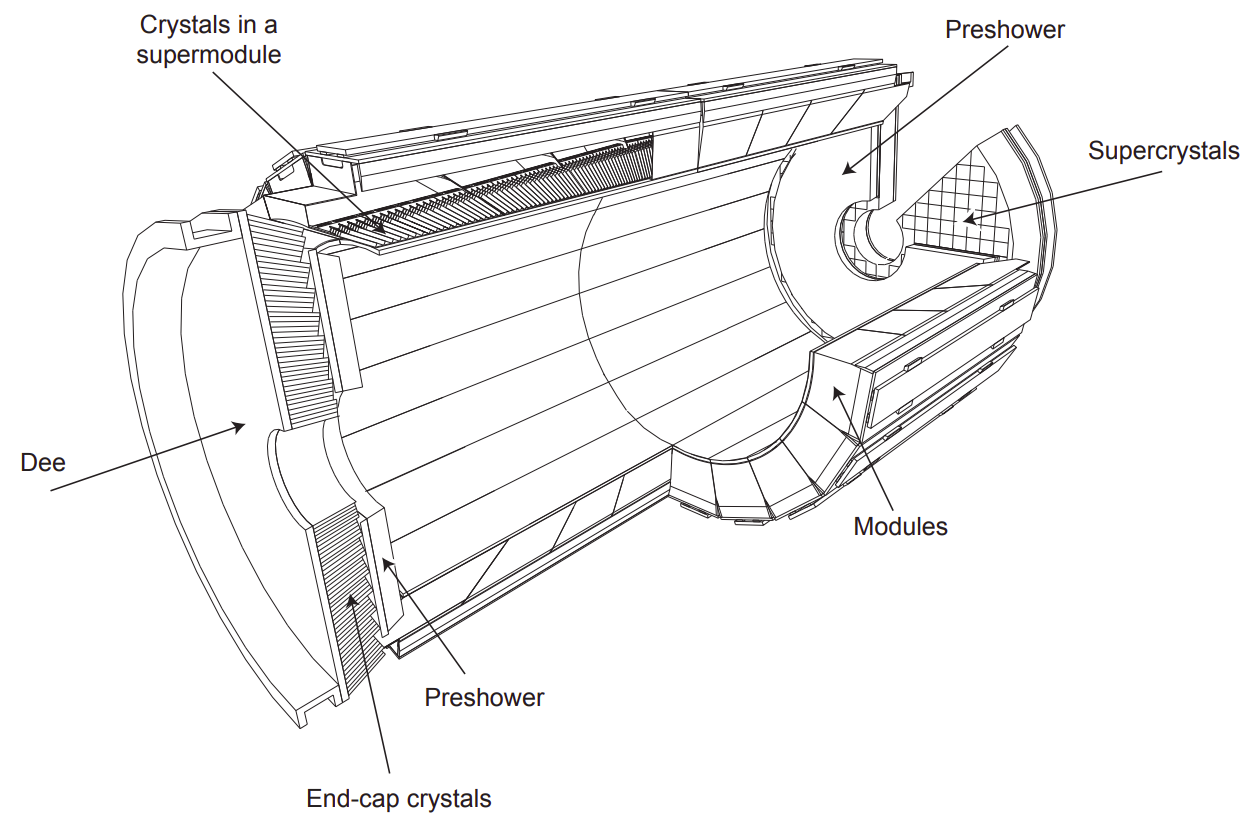
\includegraphics[width=\textwidth]{Figures/ECAL.png}
    \caption[Diagram of the CMS ECAL.]{A schematic of the CMS ECAL detector~\cite{CMS_Setup}.}
    \label{fig:ecal}
\end{figure}

\subsection{Hadronic calorimeter}

The \ac{CMS} detector includes the \ac{HCAL}~\cite{CMS_Setup,USCMS:2009fxn}, which plays a crucial role in measuring the energies of strongly interacting particles and being able to reconstruct missing energy signals. 
The \ac{HCAL} is located outside of the \ac{ECAL} and covers the pseudorapidity region $|\eta| < 5.2$. 
It consists of four sub-detectors: the \ac{HB}, \ac{HE}, \ac{HO}, and \ac{HF} calorimeters, arranged as shown in Figure~\ref{fig:hcal}. \\

\begin{figure}[!hbtp]
    \centering
    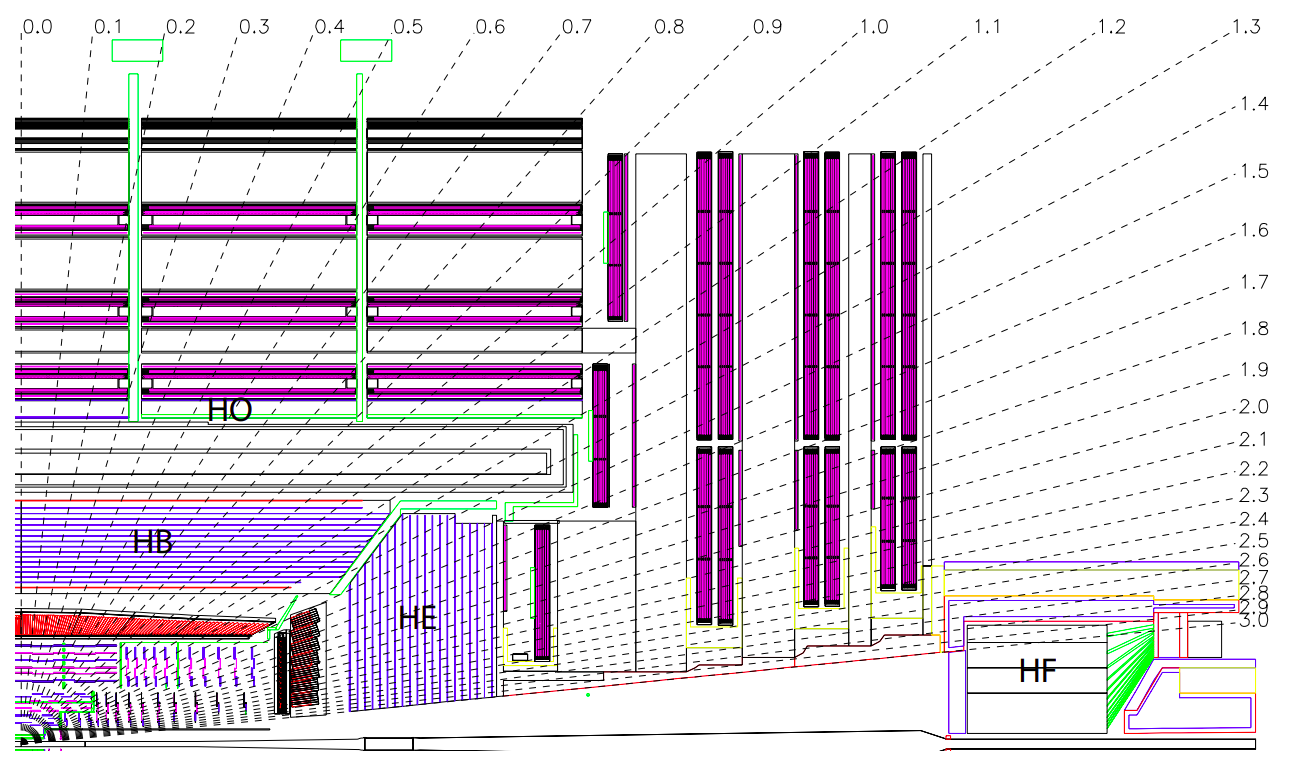
\includegraphics[width=\textwidth]{Figures/HCAL.png}
    \caption[Diagram of the CMS HCAL.]{A schematic of the CMS HCAL showing the arrangement of the HB, HE, HO, and HF calorimeters. The numbers represent the $|\eta|$ value in the detector~\cite{CMS_Setup}.}
    \label{fig:hcal}
\end{figure}

The \ac{HB} and \ac{HE} calorimeters are positioned within the magnet bore, covering the pseudorapidity regions $|\eta| < 1.3$ and $1.3 < |\eta| < 3.0$, respectively. 
They are constructed using alternating layers of brass absorber plates and plastic scintillator tiles. 
Brass is chosen as the absorber material due to its short nuclear interaction length and non-magnetic properties. 
The \ac{HB} provides 5.82 to 10.6 interaction lengths of absorber material, while the \ac{HE} provides approximately 10 interaction lengths. 
The plastic scintillator tiles collect scintillation light emitted by charged particles in the hadronic showers, which is then read out using hybrid photodiodes. \\

The \ac{HO} calorimeter extends the \ac{HCAL}'s containment capability in the central detector region ($|\eta| < 1.3$).
It is placed outside of the solenoid coil and utilises plastic scintillator tiles as the active material. 
The \ac{HO} enhances the thickness of the \ac{HCAL} to a minimum of 11.8 interaction lengths, improving the measurement of late-starting or highly penetrating showers. \\

In the forward regions ($|\eta| > 3.0$), the \ac{HF} detector extends the pseudorapidity coverage of the \ac{HCAL} up to $|\eta| < 5.2$. 
The \ac{HF} is subjected to a high flux of incoming particles, and therefore, requires extremely radiation-hard materials. 
Quartz fibres embedded in steel absorbers are employed as the active material. 
Charged particles in the showers generate Cherenkov light in the quartz fibres, which is detected by photomultiplier tubes. \\

The energy resolution of the \ac{HCAL} can be parametrised as a function of the incident particle energy E, using the formula, 

\begin{equation}
\Big(\frac{\sigma}{E}\Big)^2 = \Big(\frac{S}{\sqrt{E}}\Big)^2 + C^2
\end{equation}

where the stochastic term S was measured to be 0.943 GeV${^{1/2}}$ and the constant term C is measured to be 0.084 in the barrel~\cite{USCMS:2009fxn}.
During the \ac{LS1} period, upgrades were performed on the photomultiplier tubes of the \ac{HF}~\cite{CMS:2012tda}.

\subsection{Muon system}

The muon system in the \ac{CMS} detector~\cite{CMS_Setup,Abbiendi:2015txa} plays a crucial role in the accurate identification and measurement of muons. 
This is essential for various physics analyses. 
The system is designed with three primary functions: efficient muon identification, precise momentum measurement, and triggering capability. \\

Located outside the solenoid coil and \ac{HO} calorimeter, the muon system is strategically positioned between the iron plates forming the flux return yoke. 
This arrangement takes advantage of the high-field solenoidal magnet and the yoke's structure to enable the desired functions.
The muon system covers a pseudorapidity range of $|\eta| < 2.4$. 
It consists of three types of gaseous detectors: \ac{DT} chambers, \ac{CSC}, and \ac{RPC}. \\

In the region of $|\eta| < 1.2$, the muon system employs \ac{DT} chambers, which are organised into four stations. 
These include inner and outer stations positioned inside and outside the magnet return yoke, as well as two stations inter-spaced between the iron layers of the yoke. 
The \ac{DT} chambers are composed of rectangular drift cells, with an anode wire running through each cell and then are filled with a mixture of argon and carbon dioxide gas. 
Each cell features an anode wire running along its length. 
The cells are arranged into superlayers, each containing four layers of cells. 
The \ac{DT} chambers in the three innermost muon stations consist of three superlayers, whereas the outer station contains only two superlayers. 
The spatial resolution of the \ac{DT} chambers is measured to be 77–123 $\upmu$m for the $\phi$ coordinate measurement and 133–393 $\upmu$m for the $z$ coordinate measurement~\cite{CMS:2018rym}. \\

The \ac{CSC}s are used in the region $0.9 < |\eta| < 2.4$. 
These chambers are trapezoidal-shaped multiwire proportional chambers with six layers of gas. 
The gas mixture used includes argon, carbon dioxide, and tetrafluoromethane. 
The \ac{CSC} modules are organised into four stations positioned between the endcap layers of the magnet's return yoke. 
They consist of layers of cathode strips and anode wires, allowing for measurements of the muon's $\phi$ and $r$ coordinates, respectively. 
The spatial resolution per chamber of the \ac{CSC}s ranges from 45 $\upmu$m to 143 $\upmu$m depending on the station~\cite{CMS:2018rym}. \\

To enhance the system's capabilities in the $|\eta| < 1.6$ region, \ac{RPC}s are used. 
These parallel-plate detectors feature a double-gap module design with anode and cathode plates separated by a gas gap. 
The \ac{RPC}s are embedded within the barrel and endcap iron yokes. 
In the barrel, six layers of \ac{RPC} chambers are present, with two layers in each of the two innermost muon stations and one layer in each of the two outer stations. 
In the endcap, the \ac{RPC}s consist of four layers positioned on either side of the three iron disks. 
While the \ac{RPC}s exhibit a lower spatial resolution compared to the \ac{DT}s and \ac{CSC}s (0.78–1.38 cm per chamber), they offer a remarkably fast response time, making them suitable for dedicated muon triggering~\cite{CMS:2018rym}.

\subsection{Triggering and computing}

The \ac{LHC} collides protons at a rate of 40 MHz during its operation~\cite{Evans:2008zzb}. 
However, it is impractical to read out and store every event due to the high data volume involved. 
To address this challenge, the \ac{CMS} detector employs a dedicated trigger system that selectively chooses the most interesting events, reducing the recorded rate to around 1 kHz. \\

The \ac{CMS} trigger system consists of two stages: the \ac{L1} trigger and the \ac{HLT}~\cite{CMS_Setup,CMS_trigger,Tapper:2013yva}. 
The \ac{L1} trigger, implemented with custom-built programmable electronics, operates as the first stage and reduces the event rate from 40 MHz to approximately 100 kHz. 
During the upgrade in 2015/2016, the \ac{L1} system was enhanced to accommodate the increased instantaneous luminosity and \ac{PU} conditions~\cite{Tapper:2013yva}. 
Upgrades included improved muon momentum resolution, electron/photon isolation, hadronic tau identification and isolation, jet-finding algorithms with \ac{PU} subtraction, and enhanced trigger menu capabilities. \\

Since the beginning of Run 2, the \ac{L1} trigger utilises a time multiplexed architecture, where energy deposits recorded in the calorimeters and hits from the muon detectors are processed~\cite{Tapper:2013yva}. 
In the calorimeter trigger, energy deposits from the \ac{HCAL} and \ac{ECAL} are passed through two layers (Layer 1 and Layer 2), enabling object identification and the selection of the best candidates based on their $\pT$. 
Simultaneously, hits from the muon detectors are combined in the muon trigger's tracking finder and sorting/merging layers, producing a sorted list of muon candidates for the entire detector. 
The global trigger then integrates the information from both calorimeter and muon triggers to decide on event selection within a maximum storage time of 3.2 $\upmu$s.
A diagrammatic representation of this is shown in Figure~\ref{fig:trigger}. \\

\begin{figure}[!hbtp]
    \centering
    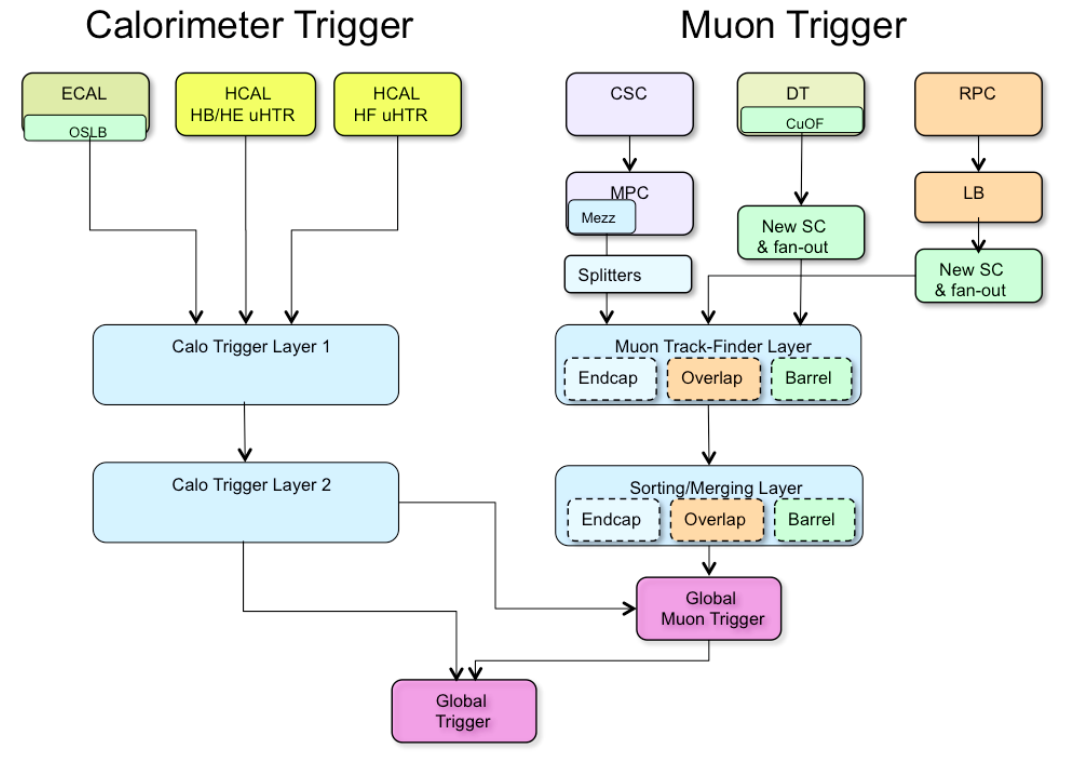
\includegraphics[width=\textwidth]{Figures/trigger.png}
    \caption[Diagram of the CMS L1 trigger workflow.]{A schematic of the L1 trigger workflow for object reconstruction~\cite{Tapper:2013yva}.}
    \label{fig:trigger}
\end{figure}

The second stage of the trigger system is the \ac{HLT}, which is a software-based trigger running on a multi-processor farm with thousands of CPU cores~\cite{CMS_trigger,CMSTrigger:2005yhe}. 
The \ac{HLT} utilises information from the full detector, including the tracker, calorimeters, and muon systems. 
By closely following the algorithms and selections used offline, the \ac{HLT} ensures good momentum resolution and high identification efficiencies for selected objects. 
From the initial event rate of approximately 100 kHz received from the \ac{L1} trigger, the \ac{HLT} further reduces the output rate to about 1 kHz. \\

The events selected by the \ac{HLT} produce a significant amount of data, approximately $\mathcal{O}$(10 pb) per year. 
To process, store, and facilitate easy access for analysts worldwide, \ac{CMS} collaborates with other \ac{LHC} experiments through the \ac{WLCG}~\cite{wlcg}. 
The \ac{WLCG} combines computing resources from research institutions globally, organised into three tiers. 
Tier-0 sites, comprising the \ac{CERN} Data Center and the Wigner Research Centre in Budapest, perform full data reconstruction and store a copy of the data on tape. 
The data is then distributed to Tier-1 centres, which handle the storage of raw, reconstructed, and simulated data, as well as the distribution to Tier-2 sites. 
Tier-2 sites, located at universities and research institutes worldwide, provide computing resources for data production, reconstruction, and analysis by researchers.

%\newpage
%\chapter{Object Reconstruction}
\label{sec:tau_identification}

\section{Tracks and vertices}

\section{Particle flow}

The particle-flow (PF) algorithm reconstructs the products of the LHC pp collisions and is described in full in Ref.\cite{PF_CMS}.  It utilises all the information available from the tracker, ECAL, HCAL and muon detectors combined to produce a list of particle candidates. These candidates are either a photon, electron, muon or a neutral or charged hadrons. It begins with defining an event as the data taken per bunch crossing. The PF algorithm then reconstructs the tracks of the particle candidates in order to find the collision vertices. The primary collision vertex is taken to be the one with the largest value of \(p_T^{2}\) summed over all physics objects originated from that vertex. Physics objects are not only defined to include particle candidate tracks, but also missing tracks represented by the negative vectorial sum of all particle candidate tracks. Other pp collisions vertices are referred to as pileup. \\

In reconstructing electron and muons, the energy deposits in the ECAL and the track hits in the muon chamber respectively, working alongside the tracker, provide the basis of electron and muon identification. However, additional requirements are used to drop misidentification rates by ensuring that the electron or muon is isolated from any hadronic activity in the detector, as leptons do not carry colour charge. This is done by defining a relative isolation variable \(I_{rel}^{e(\mu)}\) in the following way

\begin{equation}
    I_{rel}^{e(\mu)} = \frac{\sum p_{T,i} + \sum E_{T,i}}{p_T^{e(\mu)}}.
\end{equation}

The sums are over all particles included in a cone of radius \(\Delta R = \sqrt{(\Delta \eta)^2 + (\Delta \phi)^2}\) excluding the electron or muon itself. \(\Delta \eta\) and \(\Delta \phi\) are the angular distance in \(\eta\) and \(\phi\) around the electron or muon direction from the primary vertex. To remove problems with pileup, only charged particles originating from the primary vertex are included. To remove neutral particles from pileup in the cone, the \(p_T\) for neutral particles is estimated by subtracting half of the sum of the \(p_T\) of charged particle in the cone, due to the approximate ratio of charged to neutral hadron production. The cone size selected for electrons is \(\Delta R<0.3\) and the isolation variable is \(I_{\text{rel}}^{e(\mu)} < 0.1\). For muons is cone size is \(\Delta R<0.4\) and the isolation variable is \(I_{\text{rel}}^{e(\mu)} < 0.15\). \\

Jets originating from the hadronisation of b quarks, are identified using the combined secondary vertex b-tagging algorithm. This discriminates between jets originating from b quarks from other jets, utilising track impact parameters and secondary vertex related variables \cite{CMS_btag}. This plays a key part in the analysis, as b-tagging is used for categorisation purposes described in Section \ref{sec:cat_and_sig}. The missing transverse momentum, \(\vec{p}_T^{\hspace{1ex}\text{miss}}\), is also used in categorisation of events and is calculated as the negative vector sum of all PF reconstructed transverse momenta.

\section{Muons}
\section{Electrons}
\section{Jets}
\section{b jets}
\section{Missing transverse energy}
\section{Taus}

Also fundamental to this analysis is the identification of tau particles. The tau lepton is measured to have a mean lifetime of \(2.9 \times 10^{-13}\)s. This short lifetimes means that the tau lepton is not directly observable in the CMS detector.  In order to detect these particles, it is important to understand how the tau decays. Due to the heavy nature of the particle, it does not only decay leptonically, but unlike the muon, it can also decay hadronically. A list of prominent decays of the tau lepton are shown in the table below.

\begin{table}[h]
    \centering
    \begin{tabular}{|c|c|}
         \hline
         Decay Mode & Branching Fraction  \\
         \hline
         \hline
         \textbf{Leptonic Decay (\(e\), \(\mu\))} & \textbf{35.2\%} \\
         \(e^- \bar{\nu}_e \nu_\tau \) & 17.8\% \\
         \(\mu^- \bar{\nu}_\mu \nu_\tau \) & 17.4\% \\
         \hline
         \textbf{Hadronic Decay (\(\tau_h\))} & \textbf{64.8\%} \\
         \(h^- \pi^0 \nu_\tau \) & 25.9\% \\
         \(h^- \nu_\tau\) & 11.5\% \\
         \(h^- 2\pi^0 \nu_\tau\) & 9.3\% \\
         \(\pi^- \pi^- \pi^+ \nu_\tau\) & 9.0\% \\
         \(\pi^- \pi^- \pi^+ \pi^0 \nu_\tau\) & 2.7\% \\
         other & 6.4\% \\
         \hline
    \end{tabular}
    \caption{Measured branching fractions, that are greater than 2\%, for the tau lepton. h represents a charged hadron either a pion or a kaon.}
    \label{tab:tau_decay}
\end{table}

These decays can be split into three groups: the 17.8\% of taus that decay to an electron (e), the 17.4\% that decay into a muon (\(\mu\)) and hadronic tau decays (\(\tau_h\)) that make up the final 64.8\% of tau decays. The leptonic decays of the tau can be accounted for by the identification of electrons and muons as discussed in the previous subsection. The hadron-plus-strips (HPS) algorithm is used to identify hadronic taus \cite{CMS_hps1,CMS_hps2}. This algorithm groups electrons, positrons and photons and names this cluster as a "strip". This is defined to represent the decay products of the \(\pi^0\) meson. The strip size is variable depending on the \(p_T\) of its components. In a jet, the number of strips and charged particles are counted. If the numbers are corresponding to the number of \(\pi^0\) mesons and charged hadrons shown in Table \ref{tab:tau_decay} for hadronic decays, it is concluded that the jet may originate from a tau lepton. \\

To reduce misidentification, the tau lifetime is utilised. The tau lepton is expected to travel a small but identifiable distance before it decays. This distance between the decay vertex and the primary vertex is the variable used. To further reduce misidentification from the hadronisation of quarks or gluons, a similar isolation discriminant is used as for electrons and muons with \(\Delta R < 0.3\). All of these are combined into a multivariate hadronic tau identification algorithm (MVA) given in Ref.\cite{CMS_hps1}. From this reference the working points Tight, Medium and VeryLoose are used.  These refer to the output of the MVA varying the maximum values of the \(p_T\) of the hadronic tau candidate. The same MVA (excluding the HPS algorithm) is also used to reduce misidentification of leptonic tau decays. For \(\tau_h\) identification in this analysis the Tight working point is used. In order to suppress misidentification of leptonic tau decay the Tight (VeryLoose) working point for electrons and Loose (Tight) working points for muons are used in the \(e\tau_h(\mu\tau_h)\) channels. \\

For a final state of two taus, there are six possible final states: \(e\mu\), \(e\tau_h\), \(\mu \tau_h\), \(\tau_h \tau_h\), \(ee\) and  \(\mu \mu\). However, \(ee\) and \(\mu \mu\) are dominated by large backgrounds and have relatively low cross sections, so provide very little sensitivity to this analysis and hence are not included. The other four channels are all utilised.

%\newpage
\chapter{\texorpdfstring{Searches for new physics in $\tau^+\tau^-$ final states}{Search for new physics in tautau final states}}
\label{sec:bsm_H_to_tau_tau_analysis}
 
The $\tau^+\tau^-$ final states are a powerful tool to search for new physics at collider experiments. 
As the heaviest lepton, $\tau$ particles are sensitive to resonant production of new neutral particles where the couplings have a mass hierarchy.
They are also sensitive to non-resonant effects from new physics mediators. 
This chapter details the searches for two such areas of new physics: additional Higgs bosons and vector leptoquarks.
These searches are split up into three sections: 
\begin{enumerate}[i)]
  \item A model-independent search for a single narrow spin-0 resonance ($\phi$), produced via gluon fusion (gg$\phi$) or in association with a b quark (bb$\phi$). The \ac{SM} Higgs boson is treated as a background and the Yukawa couplings of the spin-0 resonance that contributes to the gluon fusion loop are set to \ac{SM} values.
   \item A search for the \ac{MSSM} Higgs sector in several benchmark scenarios. The benchmark scenarios were proposed in References~\cite{Bahl:2018zmf,Bahl:2020kwe,Bahl:2019ago} and described fully in Reference~\cite{Bagnaschi:2791954}. The $M_{h}^{125}$ and $M_{h,\text{ EFT}}^{125}$ scenarios are shown in this chapter. The production of the observed Higgs boson particle at 125 GeV is also used to constrain the available phase space.
  \item A search for the t-channel exchange of a U(1) vector leptoquark. Two scenarios are taken, motivated by the best fit to the B anomalies as detailed in Section~\ref{sec:b_anomalies}.
\end{enumerate}

These searches are performed with the full Run 2 dataset ($138 \sifb$) collected by the \ac{CMS} experiment. 
The search for additional Higgs bosons had previously been performed with data collected in 2016 ($39 \sifb$) and results were consistent with the \ac{SM} background prediction \cite{CMS_MSSM_Tau_2018}.
 
\section{Signal modelling} 
 
\subsection{Additional Higgs bosons} 
\label{sec:additional_higgs_bosons} 
 
Extended Higgs sectors, such as that of the \ac{MSSM}, can be probed by direct searches for the additional bosons and further precise measurements of the \ac{SM} Higgs boson. 
This search for an extended Higgs sector is motivated by a Type II \ac{2HDM}, such as the \ac{MSSM}.
In these models, $\tan\beta$ enhances couplings of additional Higgs bosons to down-type quarks and charged leptons, whilst up-type quark couplings are suppressed.
This divides the dominant production modes of the Higgs boson into two categories: gluon fusion and production in association with a b quark.
Examples of the Feynman diagrams for these processes are shown in Figure~\ref{fig:mssm_feynamn}, where $\phi$ can represent any of the additional neutral Higgs bosons ($\Ph$, $\PH$ or $\PA$) in these diagrams.\\

\begin{figure}[H]
\centering
\begin{subfigure}[b]{0.3\textwidth}
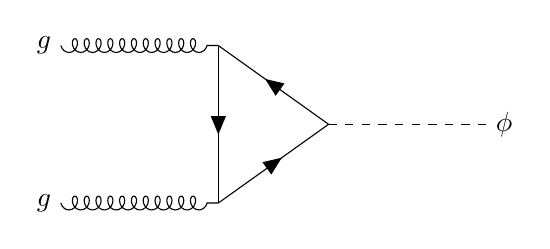
\begin{tikzpicture}[scale=2]
  \begin{feynman}
    \vertex [label=left:$g$] (a1) at (0,0);
    \vertex [label=left:$g$] (a2) at (0,1);
    \vertex (b1) at (1,0);
    \vertex (b2) at (1,1);
    \vertex (c) at (1.7,0.5);
    \vertex [label=right:$\phi$] (d) at (2.7,0.5);

    \diagram* {
      (a1) -- [gluon] (b1),
      (a2) -- [gluon] (b2),
      (b2) -- [fermion] (b1),
      (c) -- [fermion] (b2),
      (b1) -- [fermion] (c),
      (c) -- [scalar] (d),
    };
  \end{feynman}
\end{tikzpicture}
\caption{}
\end{subfigure}


\begin{subfigure}[b]{0.3\textwidth}
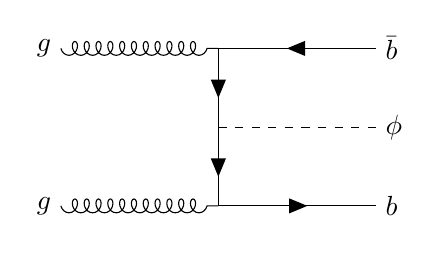
\begin{tikzpicture}[scale=2]
  \begin{feynman}
    \vertex [label=left:$g$] (a1) at (0,0);
    \vertex [label=left:$g$] (a2) at (0,1);
    \vertex (b1) at (1,0);
    \vertex (b2) at (1,0.5);
    \vertex (b3) at (1,1);
    \vertex [label=right:$b$] (c1) at (2,0);
    \vertex [label=right:$\phi$] (c2) at (2,0.5);
    \vertex [label=right:$\bar{b}$] (c3) at (2,1);
    \diagram* {
      (a1) -- [gluon] (b1),
      (a2) -- [gluon] (b3),
      (b3) -- [fermion] (b2),
      (b2) -- [fermion] (b1),
      (c3) -- [fermion] (b3),
      (b1) -- [fermion] (c1),
      (b2) -- [scalar] (c2),
    };
  \end{feynman}
\end{tikzpicture}
\caption{}
\end{subfigure}
\hspace{2cm}
\begin{subfigure}[b]{0.3\textwidth}
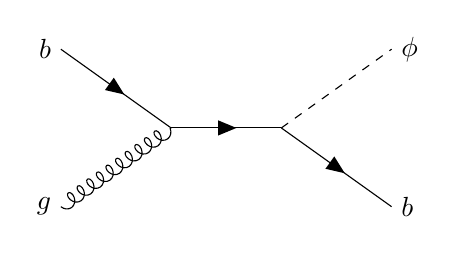
\begin{tikzpicture}[scale=2]
  \begin{feynman}
    \vertex [label=left:$g$] (a1) at (0,0);
    \vertex [label=left:$b$] (a2) at (0,1);
    \vertex (b) at (0.7,0.5);
    \vertex (c) at (1.4,0.5);
    \vertex [label=right:$b$] (d1) at (2.1,0);
    \vertex [label=right:$\phi$] (d2) at (2.1,1);
    \diagram* {
      (a1) -- [gluon] (b),
      (a2) -- [fermion] (b),
      (b) -- [fermion] (c),
      (c) -- [fermion] (d1),
      (c) -- [scalar] (d2),
    };
  \end{feynman}
\end{tikzpicture}
\caption{}
\end{subfigure}
\vspace*{10mm}
\caption[Feynman diagrams for gluon fusion and production in association with b quarks.]{Diagram (a) shows the production of neutral Higgs bosons from gluon fusion. The dominant loop contributions to these diagrams are from t-only, b-only and tb-interference. Diagrams (b) and (c) show production in association with b quarks.}
\label{fig:mssm_feynamn}
\end{figure}

With the $\tan\beta$ enhancement, the decays of additional Higgs bosons to $\tau$ leptons and b quarks are most dominant.
$\tau$ leptons are identified with higher purity than b quarks at the \ac{CMS} detector.
It is also easier to separate $\tau^{+}\tau^{-}$ from the large \ac{QCD} multijet background produced from the high-energy proton-proton collisions.
This was confirmed with the 2016 dataset and although no deviations were observed, the strongest limits on the \ac{MSSM} phase space were placed by the $\tau^+\tau^-$ final states \cite{CMS_MSSM_Tau_2018,CMS:2018hir}. \\

For this analysis, signal templates for the production of additional Higgs bosons over a mass range of 60 GeV to 3.5 TeV are generated.
Gluon fusion is simulated at \ac{NLO} precision using the \ac{2HDM} implementation of \POWHEG 2.0~\cite{Nason:2004rx,Frixione:2007vw,Alioli:2010xd,Jezo:2015aia}.
The kinematic properties are highly dependent on the contributions to the loop, and these are dependent on the specific signal model.
To account for the t quark only, b quark only, and tb-interference loop contributions at the \ac{NLO} plus parton shower prediction, weights are calculated from the $\pT$ spectra to split these contributions up.
Once individual templates have been determined for each contribution to the loop, the \ac{2HDM} samples can be scaled to the \ac{MSSM} scenario prediction with the following formula,

\begin{align}
& \frac{d\sigma_{\text{MSSM}}}{d\pT}  = \left(\frac{Y_{t,\text{MSSM}}}{Y_{t,\text{2HDM}}}\right)^{2}\frac{d\sigma^{t}_{\text{2HDM}}}{d\pT}(Q_{t}) + \left(\frac{Y_{b,\text{MSSM}}}{Y_{b,\text{2HDM}}}\right)^{2}\frac{d\sigma^{b}_{\text{2HDM}}}{d\pT}(Q_{b}) \nonumber \\
& + \left(\frac{Y_{t,\text{MSSM}}}{Y_{t,\text{2HDM}}}\frac{Y_{b,\text{MSSM}}}{Y_{b,\text{2HDM}}}\right) \left\{ \frac{d\sigma^{t+b}_{\text{2HDM}}}{d\pT}(Q_{tb}) - \frac{d\sigma^{t}_{\text{2HDM}}}{d\pT}(Q_{tb}) - \frac{d\sigma^{b}_{\text{2HDM}}}{d\pT}(Q_{tb}) \right\} ,
\label{eqn:mssm_xs}
\end{align}
\vspace{0.2cm}

where $Q_i$ are resummation scales that depend on the mass of the additional Higgs boson, and $\sigma^{i}_{j}$ and $Y^{i}_{j}$ are the determined cross-sections and Yukawa couplings of the relevant theory $j$ and contribution $i$.
Further contributions from any supersymmetric partners were checked and accounted for less than a few percent and so are neglected.
The $\pT$ reweighting is done separately for the scalar and pseudoscalar additional Higgs bosons, as the $\pT$ distributions can differ.
The benchmark scenarios provide the relative Yukawa couplings (to calculate the cross-sections) and branching fractions of the \ac{MSSM} Higgs bosons.
An example of the distributions for gluon fusion production, in the \ac{MSSM} $M_{h}^{125}$ scenario with $m_{A} = 500$ GeV whilst varying $\tan\beta$, is shown in Figure~\ref{fig:mssm_sig}.
The distributions peak at a higher $\pT$ for the t quark loop, therefore at smaller $\tan\beta$, where the t quark contribution is dominant, an additional Higgs boson would be more boosted. \\

\begin{figure}[!hbtp]
\centering
    \subfloat[]{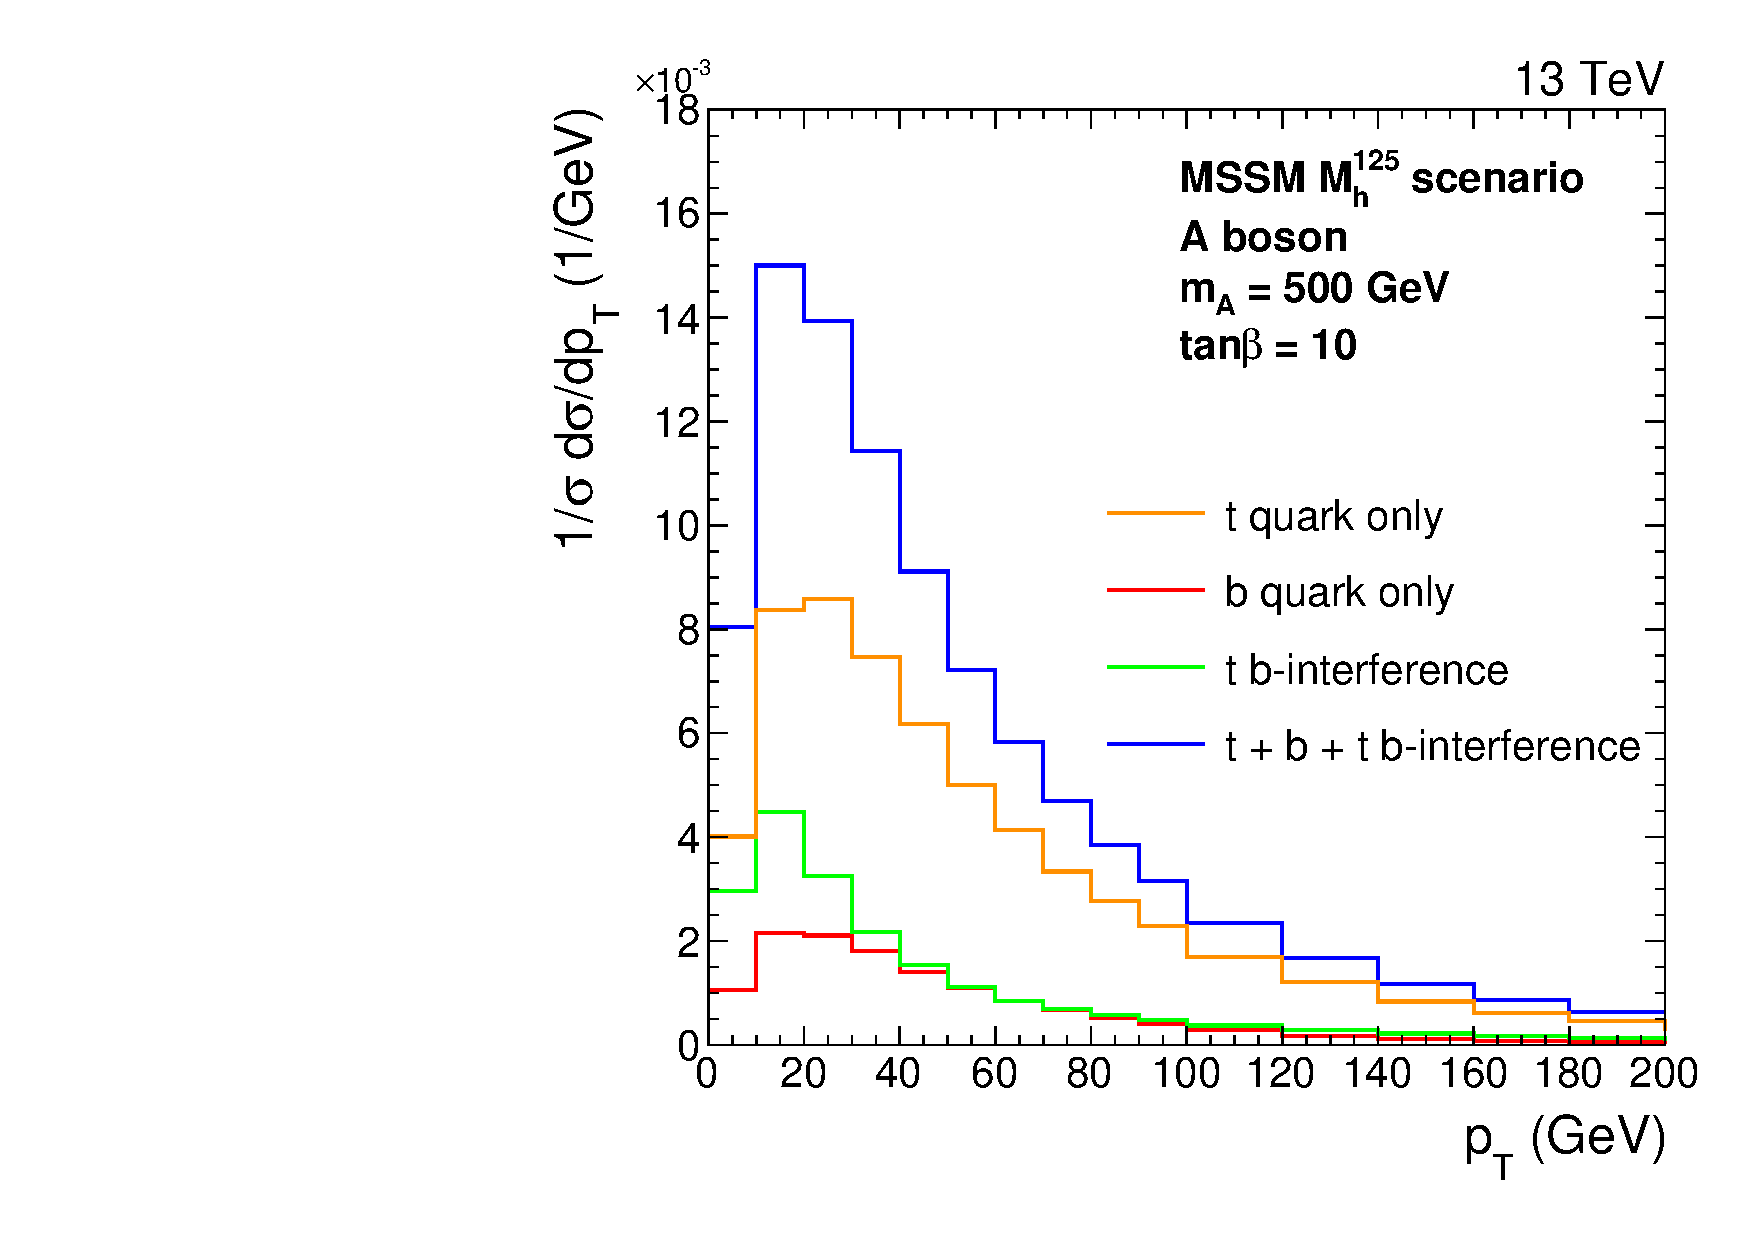
\includegraphics[width=0.5\textwidth]{Figures/pT_reweighting_plot_A10.pdf}}
    \subfloat[]{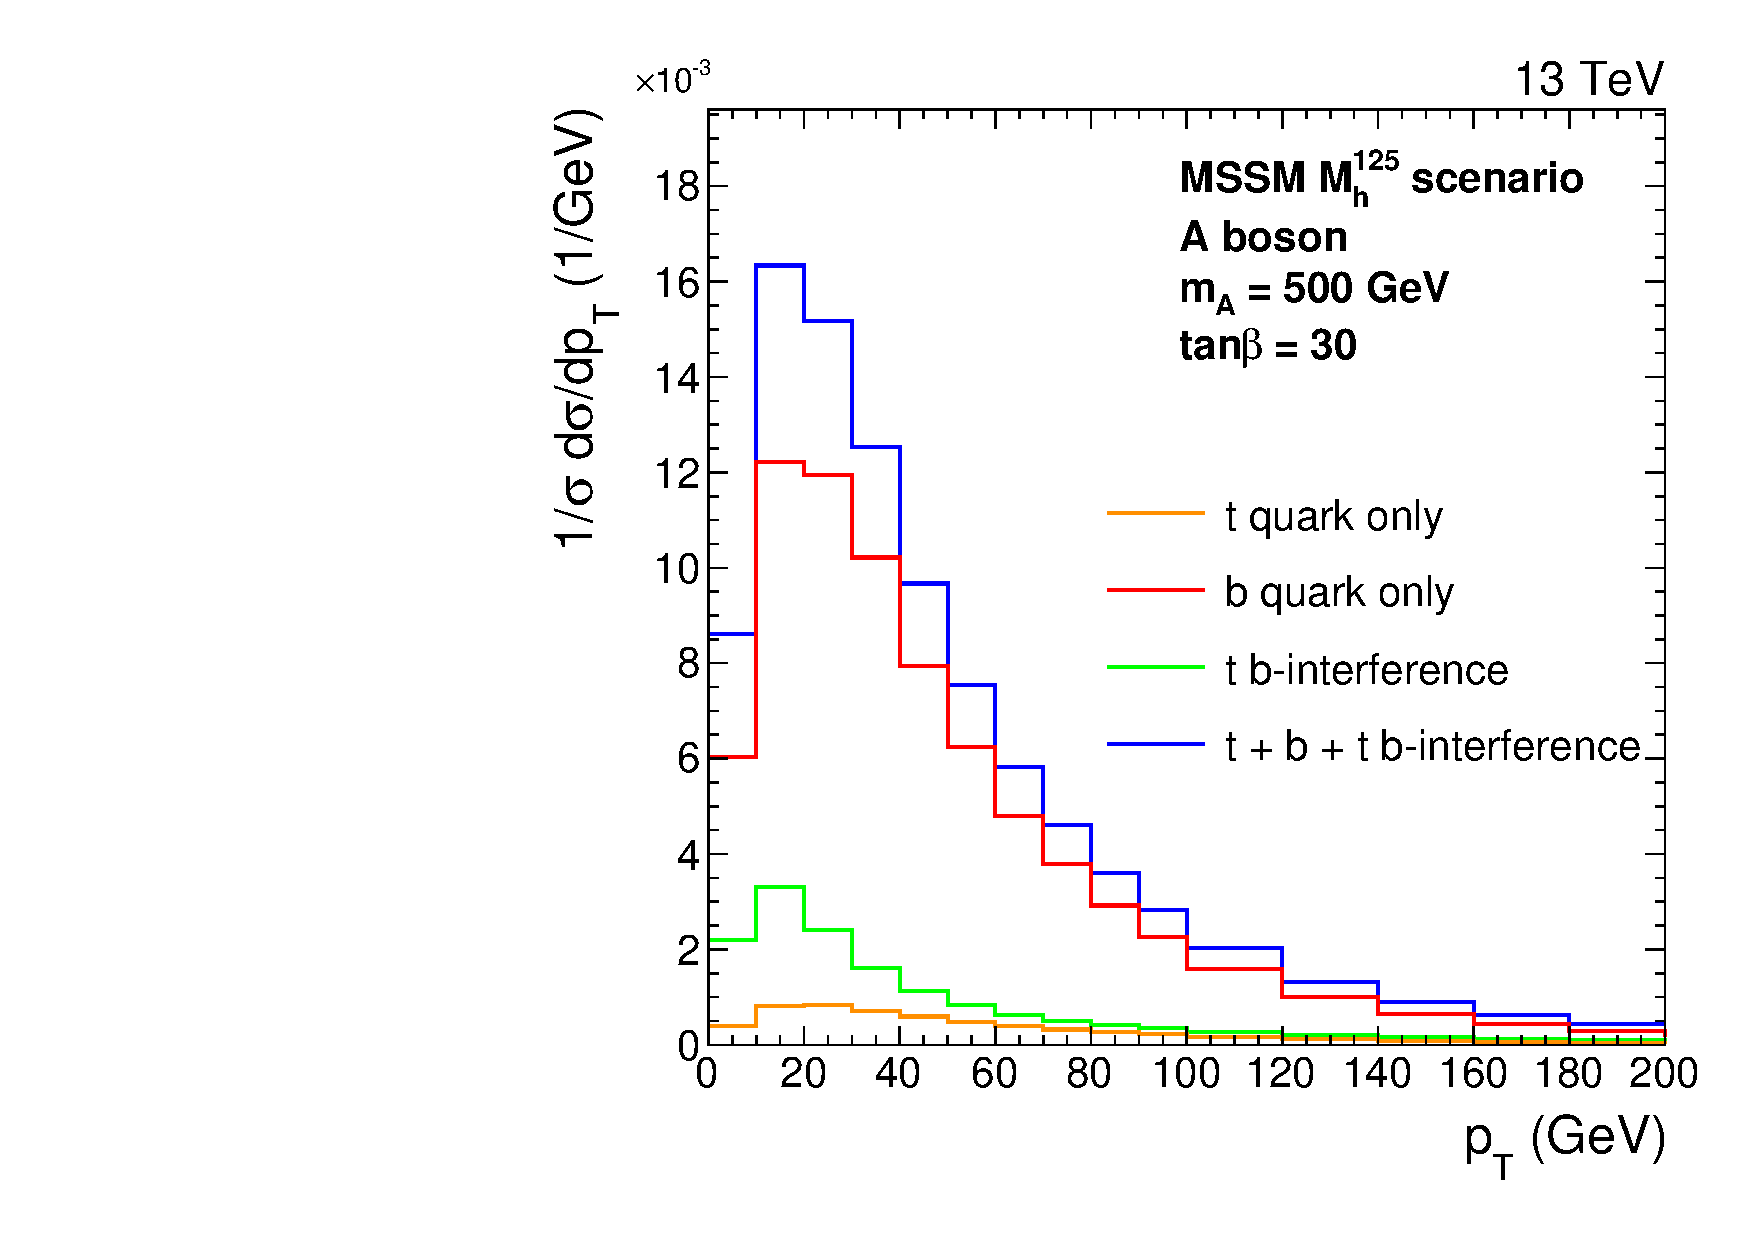
\includegraphics[width=0.5\textwidth]{Figures/pT_reweighting_plot_A30.pdf}} \\
    \subfloat[]{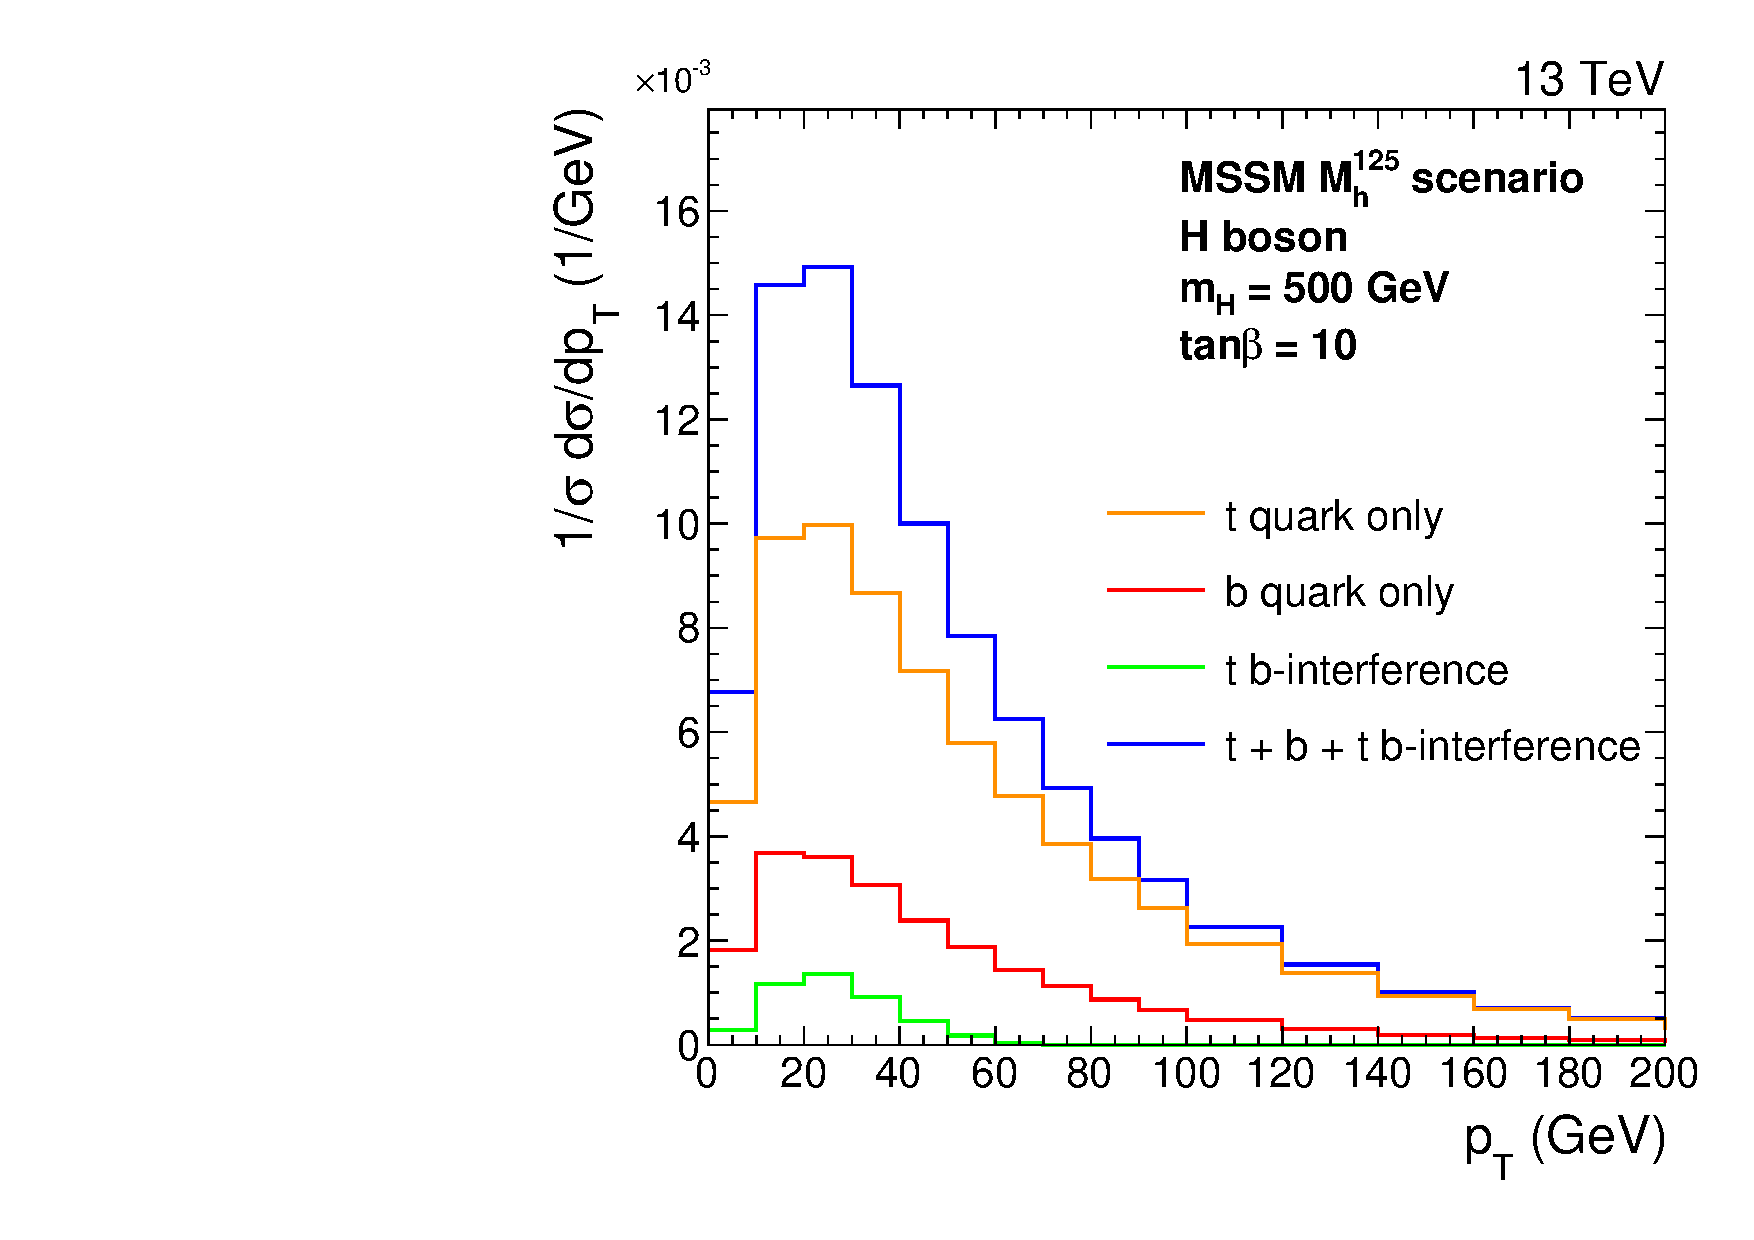
\includegraphics[width=0.5\textwidth]{Figures/pT_reweighting_plot_H10.pdf}}
    \subfloat[]{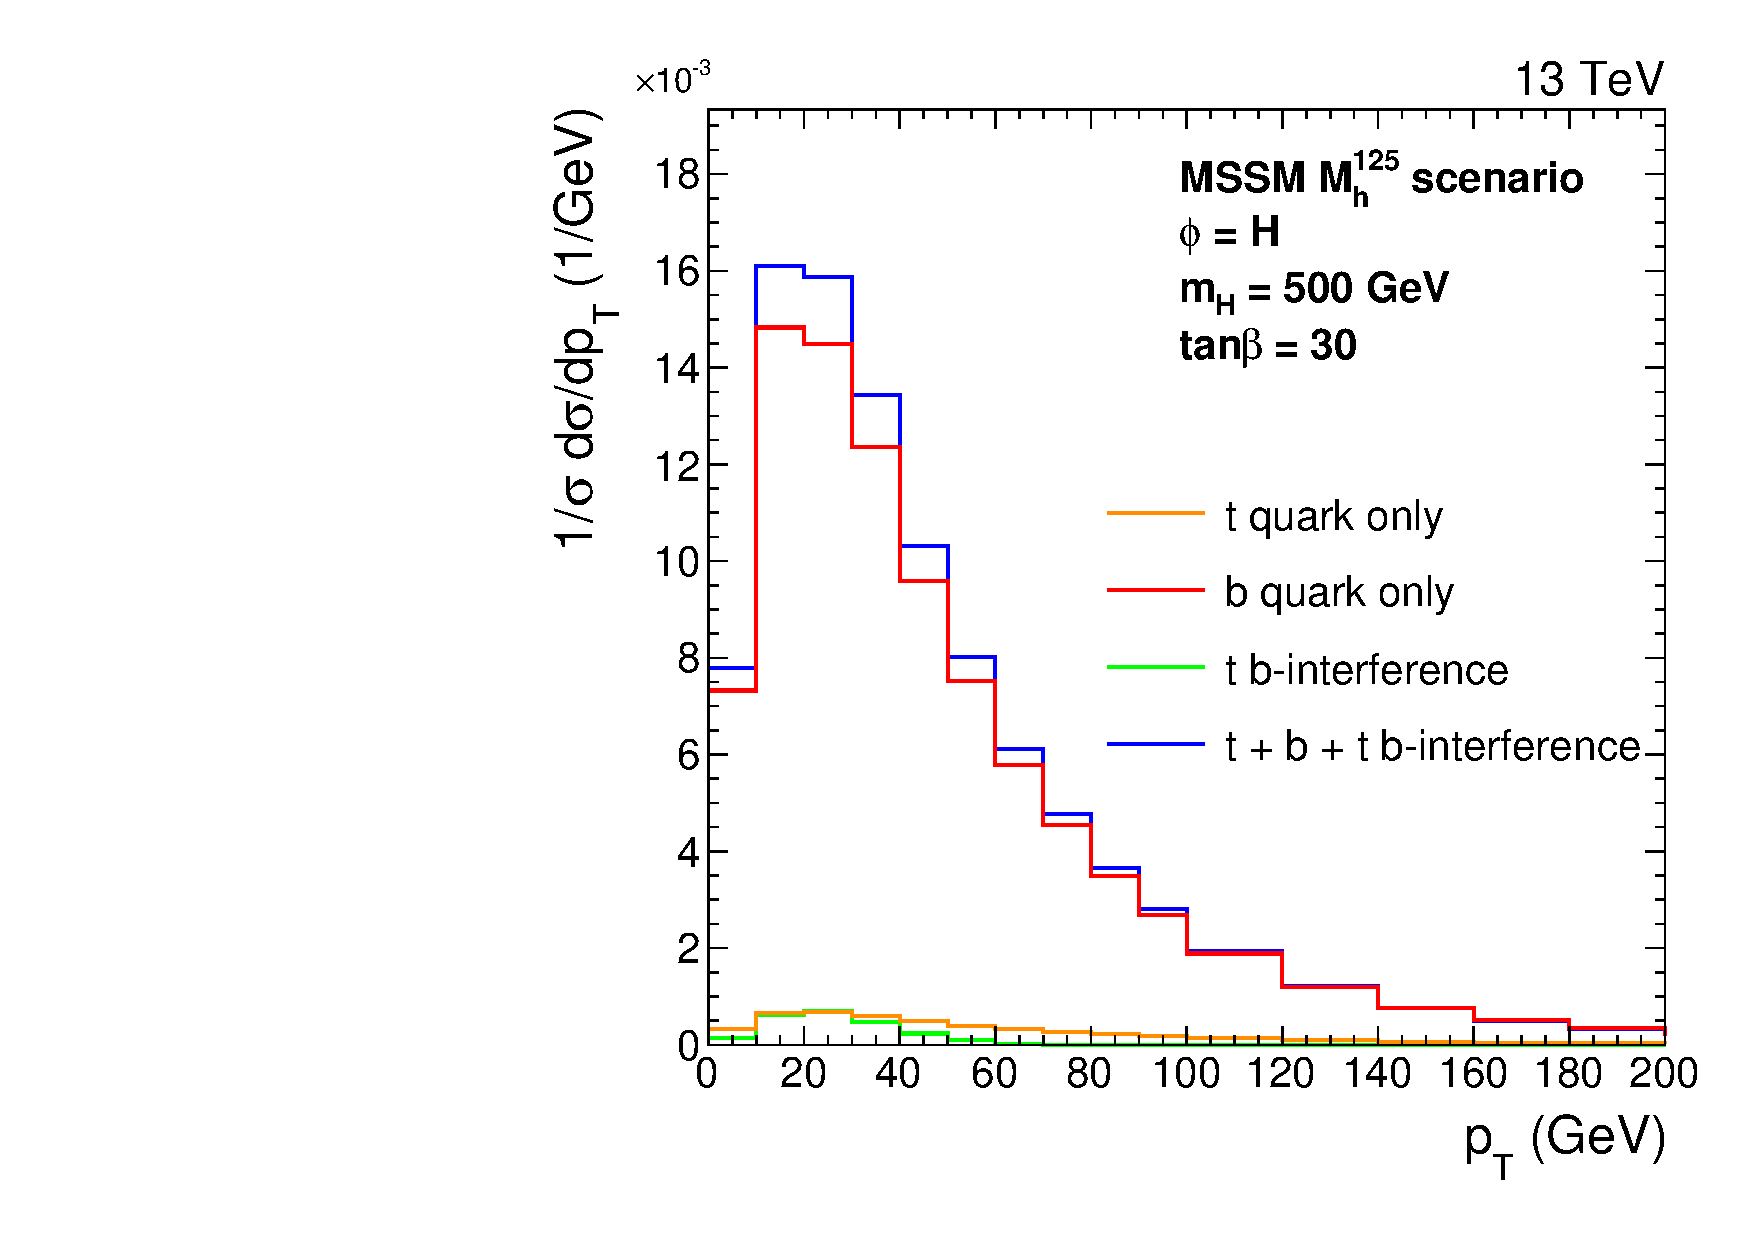
\includegraphics[width=0.5\textwidth]{Figures/pT_reweighting_plot_H30.pdf}} \\
\caption[Plots of the gluon fusion generator level $\pT$ distributions, when changing the MSSM parameters.]{$p_{T}$ density distributions of the A (top) and H (bottom) boson, with contributions to the gluon fusion loop displayed individually and summed. These are shown for $\tan\beta$ values of 10 (left) and 30 (right) where $m_{A} = 500$ GeV in the MSSM $M_{h}^{125}$ scenario.}
\label{fig:mssm_sig}
\end{figure}

Production in association with b quarks is simulated at \ac{NLO} precision using the corresponding \POWHEG 2.0 implementation in the four \ac{FS}~\cite{Nason:2004rx,Frixione:2007vw,Alioli:2010xd,Jezo:2015aia}.
All additional Higgs boson signal generation is performed using the parton distribution function NNPDF3.1~\cite{Ball:2014uwa,Ball:2017nwa}.
$\tau$ lepton decay, parton showering and hadronisation are all modelled with the \PYTHIA event generator where the \ac{PU} profile is matched to data~\cite{Sirunyan:2019dfx,Sjostrand:2014zea}.
All events generated are passed through a \texttt{GEANT4}-based \cite{Agostinelli:2002hh} simulation of the \ac{CMS} detector and reconstructed in the same way as data. \\

The model-independent and model-dependent additional neutral Higgs boson searches explained in this chapter, utilise the same signal templates generated. 
The differences lie in the scaling of the gluon fusion cross-section and loop contributions (set to the Yukawa couplings for the model-independent interpretation), and the b associated production cross-section, as well as taking into account the branching fractions in the model-dependent interpretation.
The model-dependent search for the \ac{MSSM} also looks to find differences between the observed \ac{SM} Higgs boson and the predicted \ac{MSSM} \ac{SM}-like Higgs boson.
In each \ac{MSSM} benchmark scenario, an uncertainty of $\pm 3$ GeV is given on the prediction for the \ac{SM} Higgs boson mass.
This uncertainty is to reflect the contribution of any unknown higher-order corrections.
The value of the mass is allowed to vary within this window, however, the Yukawa couplings are rescaled to that of the observed mass.

\subsection{Vector leptoquarks}
\label{sec:vlq}

The best fit to the B anomalies in the available phase space for vector leptoquarks yielded a large b quark and $\tau$ lepton coupling to the U(1) particle.
The possible production modes of a $\tau^+\tau^-$ final state are shown in Figure~\ref{fig:leptoquark_feynman}. \\

\begin{figure}[t]
\centering
\begin{subfigure}[b]{0.3\textwidth}
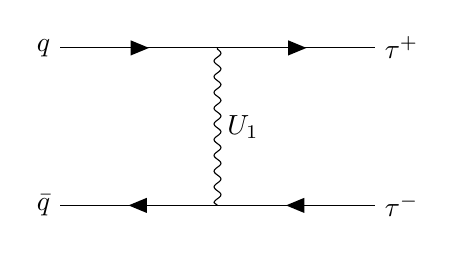
\begin{tikzpicture}[scale=2]
  \begin{feynman}
    \vertex [label=left:$\bar{q}$] (a1) at (0,0);
    \vertex [label=left:$q$] (a2) at (0,1);
    \vertex (b1) at (1,0);
    \vertex (b2) at (1,1);
    \vertex [label=right:$U_{1}$] (b3) at (1,0.5);
    \vertex [label=right:$\tau^-$] (c1) at (2,0);
    \vertex [label=right:$\tau^+$] (c2) at (2,1);

    \diagram* {
      (b1) -- [fermion] (a1),
      (a2) -- [fermion] (b2),
      (b2) -- [boson] (b1),
      (c1) -- [fermion] (b1),
      (b2) -- [fermion] (c2),
    };
  \end{feynman}
\end{tikzpicture}
\caption{}
\end{subfigure} \\

\begin{subfigure}[b]{0.3\textwidth}
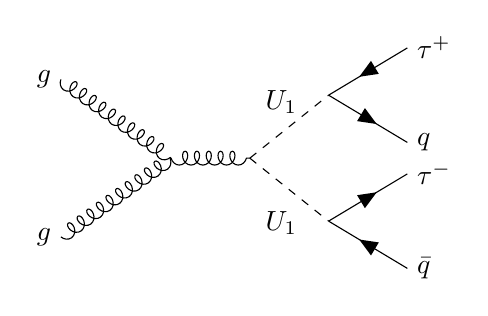
\begin{tikzpicture}[scale=2]
  \begin{feynman}
    \vertex [label=left:$g$] (a1) at (0,0);
    \vertex [label=left:$g$] (a2) at (0,1);
    \vertex (b1) at (0.7,0.5);
    \vertex (b2) at (1.2,0.5);
    \vertex (c1) at (1.7,0.1);
    \vertex (c2) at (1.7,0.9);
    \vertex [label=$U_{1}$] (c1t) at (1.4,-0.05);
    \vertex [label=$U_{1}$] (c2t) at (1.4,0.72);
    \vertex [label=right:$\tau^+$] (d1) at (2.2,1.2);
    \vertex [label=right:$q$] (d2) at (2.2,0.6);
    \vertex [label=right:$\tau^-$] (d3) at (2.2,0.4);
    \vertex [label=right:$\bar{q}$] (d4) at (2.2,-0.2);
    
    \diagram* {
      (a1) -- [gluon] (b1),
      (a2) -- [gluon] (b1),
      (b1) -- [gluon] (b2),
      (b2) -- [scalar] (c1),
      (b2) -- [scalar] (c2),
      (d1) -- [fermion] (c2),
      (c2) -- [fermion] (d2),
      (c1) -- [fermion] (d3),
      (d4) -- [fermion] (c1),
    };
  \end{feynman}
\end{tikzpicture}
\caption{}
\end{subfigure}
\hspace{2cm}
\begin{subfigure}[b]{0.3\textwidth}
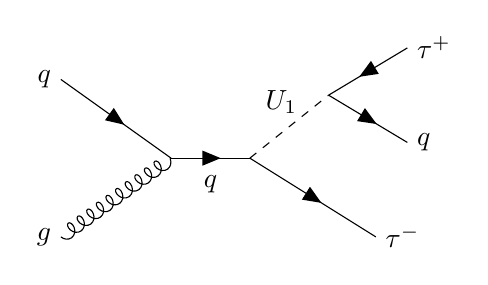
\begin{tikzpicture}[scale=2]
  \begin{feynman}
    \vertex [label=left:$g$] (a1) at (0,0);
    \vertex [label=left:$q$] (a2) at (0,1);
    \vertex (b1) at (0.7,0.5);
    \vertex [label=below:$q$] (bt) at (0.95,0.45);
    \vertex (b2) at (1.2,0.5);
    \vertex [label=right:$\tau^-$] (c1) at (2,0);
    \vertex (c2) at (1.7,0.9);
    \vertex [label=$U_{1}$] (c2t) at (1.4,0.72);
    \vertex [label=right:$\tau^+$] (d1) at (2.2,1.2);
    \vertex [label=right:$q$] (d2) at (2.2,0.6);

   
    \diagram* {
      (a1) -- [gluon] (b1),
      (a2) -- [fermion] (b1),
      (b1) -- [fermion] (b2),
      (b2) -- [fermion] (c1),
      (b2) -- [scalar] (c2),
      (d1) -- [fermion] (c2),
      (c2) -- [fermion] (d2),
    };
  \end{feynman}
\end{tikzpicture}
\caption{}
\end{subfigure}
\vspace*{10mm}
\caption[Feynman diagrams for the production of a di-$\tau$ final state from vector leptoquarks.]{Feynman diagrams showing the contribution from U(1) vector leptoquarks to the final state with a pair of oppositely charged $\tau$ leptons. $q$ represents any SM quark. The t-channel (a), pair (b) and single (c) productions of a vector leptoquark are shown.}
\label{fig:leptoquark_feynman}
\end{figure}

Pair and single production of a vector leptoquark are dependent on its strong coupling, which is highly model dependent.
For large mass, $m_U$, the probability of producing an on-shell U(1) singlet or pair is heavily suppressed due to the momentum of the initial partons.
These production processes are not discussed further in this chapter.
A search for single and pair production at the \ac{CMS} experiment was performed and no statistically significant deviation was observed~\cite{CMS:2022zks}.
Single production places the loosest constraints on the available phase space, out of the processes mentioned.
Pair production puts a lower limit on the leptoquark mass, as the process is approximately independent of $g_U$. 
However, this limit is heavily dependent on the value chosen for the strong coupling. \\

The t-channel process contains two vertices with a U(1) vector leptoquark, a quark and a $\tau$ lepton, and hence the cross-section will scale with $g_{U}^4$ ($g_{U}^2$ for each vertex).
From the best fit to B anomalies, the vertex is dominated by the b quark and hence the initial state will be mostly from $b\bar{b}$, with sub-dominant contributions from $b\bar{s}$, $s\bar{b}$ and $s\bar{s}$.
Although there are no additional b quarks in the final state in the \ac{LO} process, the production of initial state b quarks can lead to additional b quarks in the final state.
In this search, the two scenarios discussed in Section~\ref{sec:b_anomalies} are considered.
The only non-negligible freely floating parameter in each fit, for $\tau^{+}\tau^{-}$ final states in the $m_{U}$-$g_{U}$ phase space is the $\beta_{L}^{s\tau}$ parameter.
This is set to the best-fit value. \\

The signal process of a t-channel exchange is simulated in the five \ac{FS} at \ac{LO} precision using the \MGvATNLO v2.6.5 event generator~\cite{Alwall:2011uj}.
Events are generated with one or fewer outgoing partons from the matrix element and the MLM prescription~\cite{Frederix:2012ps} is then used for matching, with a scale set to 40 GeV.
Negligible dependence of the decay width is observed. 
For simulation, this is chosen to approximately match the value predicted by the B anomaly fit~\cite{Cornella:2021sby}.
Samples with a mass between 1 and 5 TeV are generated. \\

The interference between the signal and $Z/\gamma^* \rightarrow \tau\tau$ process was checked and a large destructive effect was observed, with magnitude dependent on $g_{U}$.
To account for this, separate samples are produced for this interference, using the same generators as the t-channel exchange.
The interference samples are generated with extra statistics at large di-$\tau$ mass values, to have a sufficient number of events in the regions of interest for the signal.
The cross-section of these interference samples scales with $g_{U}^2$. 
Examples of the generator level di-$\tau$ mass distributions are shown in Figure~\ref{fig:vlq_signal}. \\

\begin{figure}[!hbtp]
\centering
    \subfloat[]{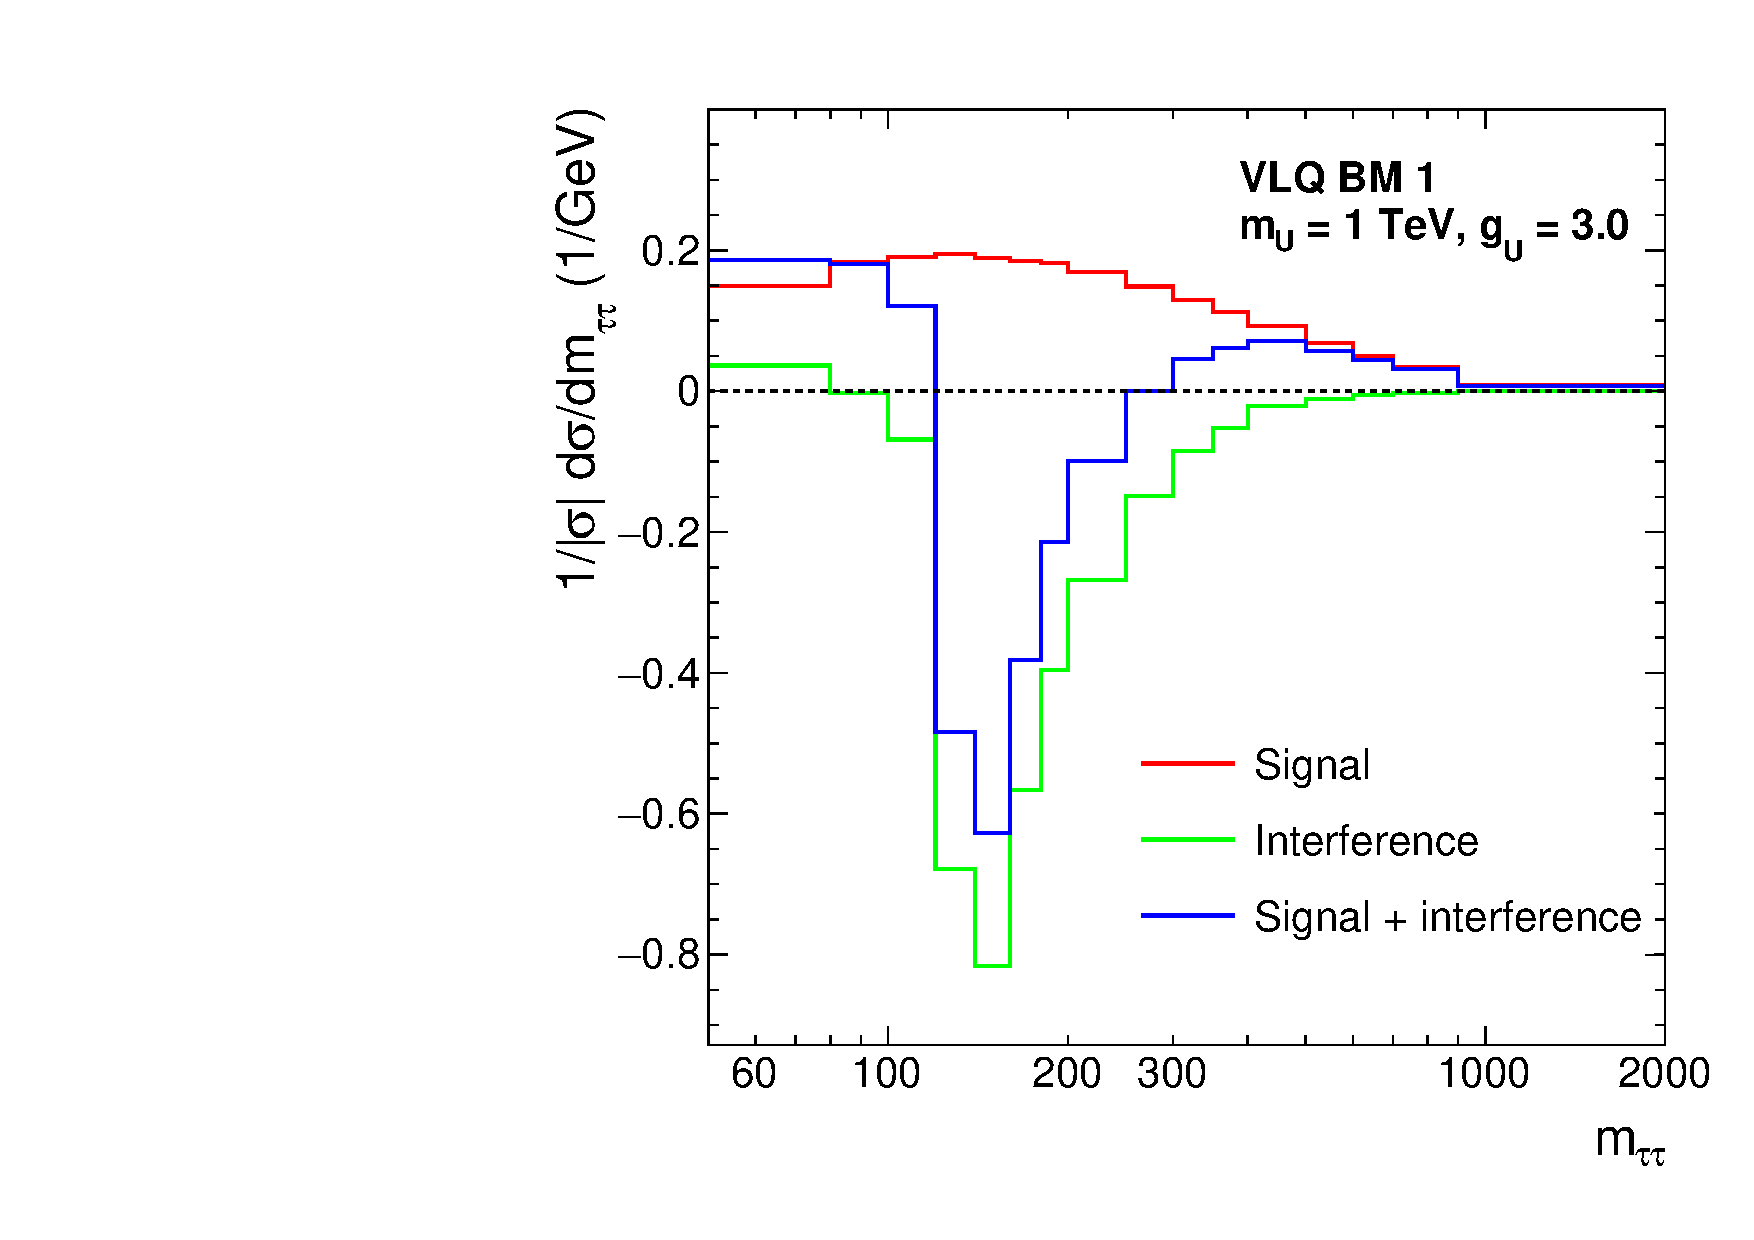
\includegraphics[width=0.5\textwidth]{Figures/vlq_signal_plot_gU3.pdf}}
    \subfloat[]{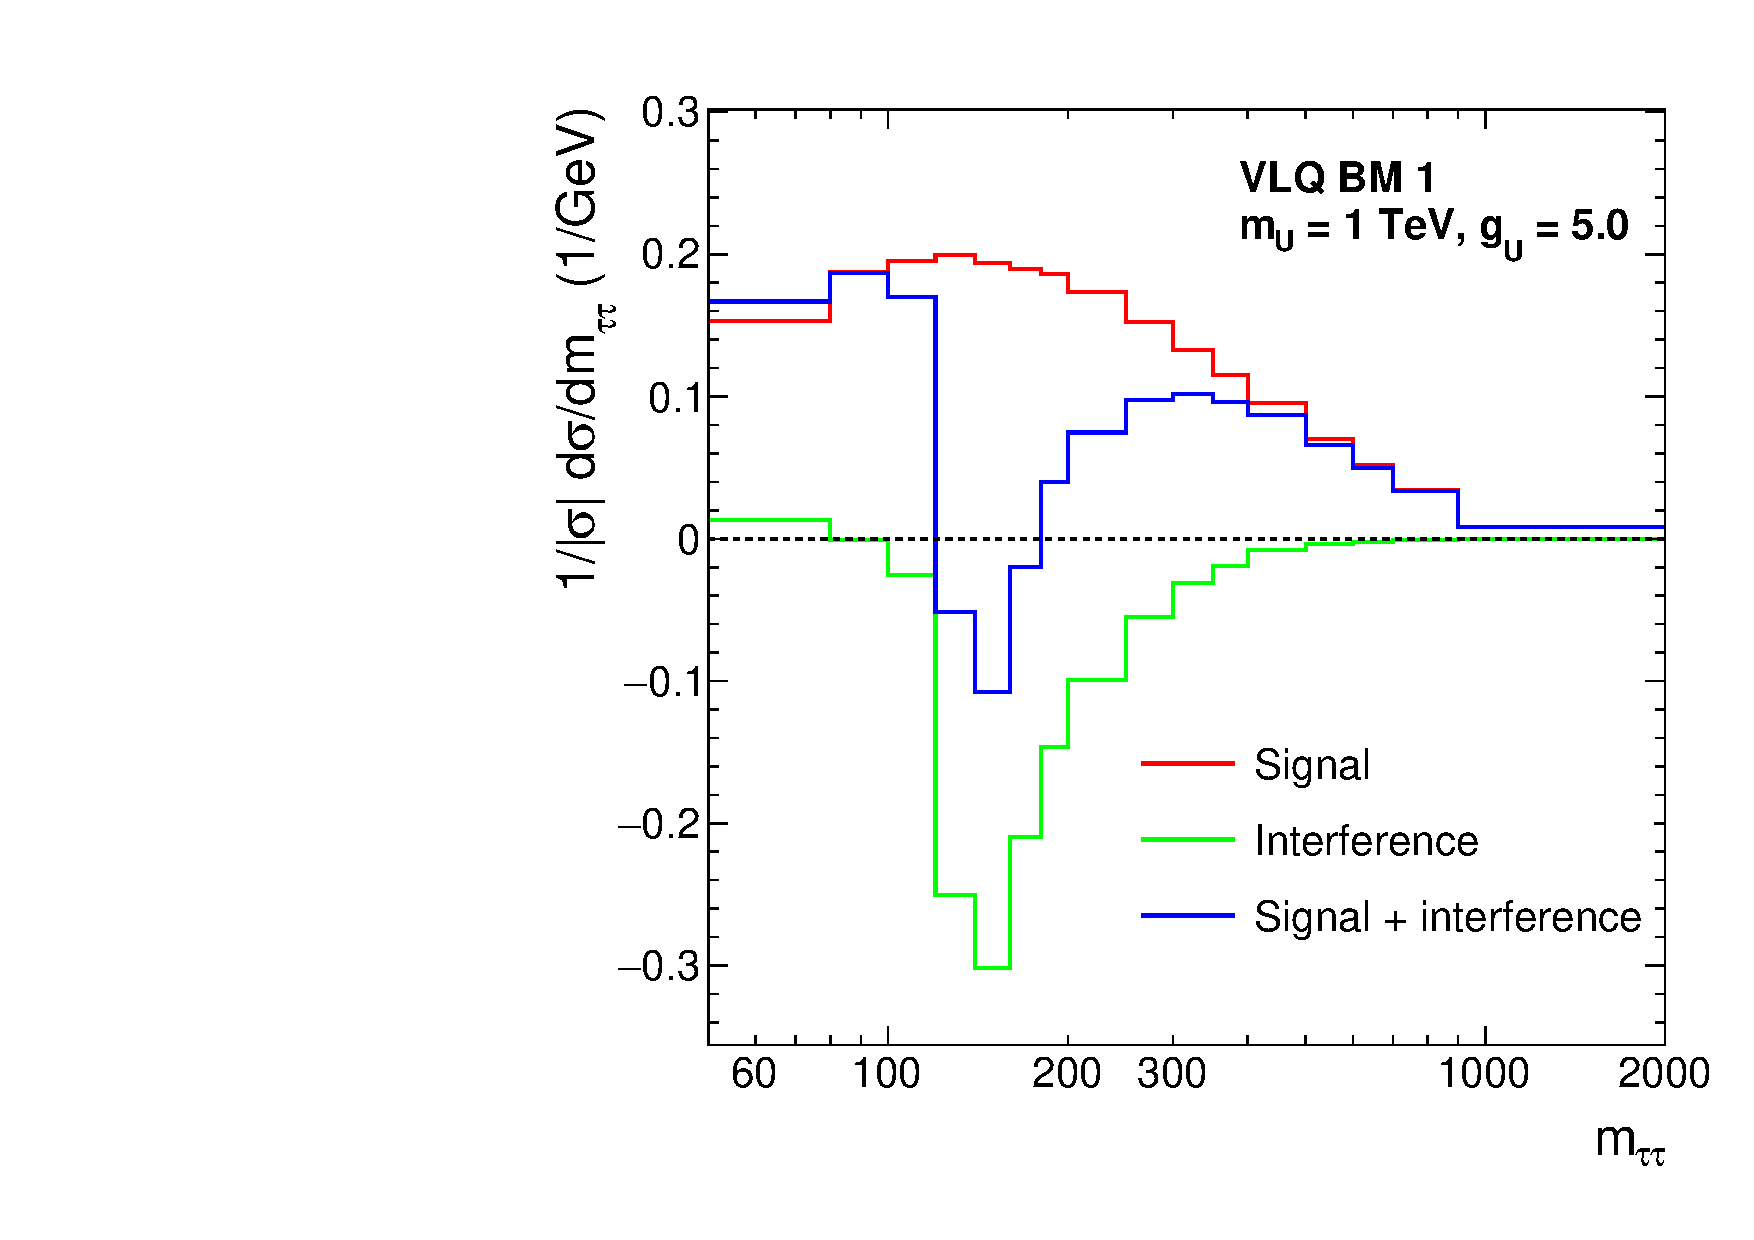
\includegraphics[width=0.5\textwidth]{Figures/vlq_signal_plot_gU5.pdf}}
\caption[Plots of the vector leptoquark generator level $m_{\tau\tau}$ distributions, when changing $g_{U}$.]{The generator level $m_{\tau\tau}$ density distributions of the t-channel vector leptoquark signal and the interference with $Z/\gamma^* \rightarrow \tau\tau$. This is shown in the VLQ BM 1 scenario for a leptoquark of mass 1 TeV for coupling strengths of $g_{U}=3$ (a) and $g_{U}=5$ (b).}
\label{fig:vlq_signal}
\end{figure}

The t-channel signal produces a broad distribution in $m_{\tau\tau}$ due to its non-resonant nature.
The interference is mostly a destructive effect (except for at small $m_{\tau\tau}$), with the yield becoming less negative at higher $m_{\tau\tau}$.
The interference peaks negatively between 100 and 200 GeV and in this region, the combined yield can be negative.
This negative signal yield would diminish the $Z/\gamma^{*}$ background.
Due to the difference in the scaling of the two effects, at small $g_{U}$ the interference is more dominant than the signal and hence the yield of the combined result is reduced.

\section{Event selection}

The possible decays of two $\tau$ leptons and their branching fractions, where the $\tau$ decay is grouped into three categories; $e$, $\mu$ and $\tau_h$ as defined in Section~\ref{sec:object_reconstruction}, are shown in Table~\ref{tab:ditau_br}. 
For this search, the four largest branching fraction channels are used: $\tauhtauh$, $\etauh$, $\mutauh$ and $e\mu$.
This accounts for approximately 94\% of di-$\tau$ events.
The two same lepton channels are neglected due to the small branching ratio and the dominating $Z\rightarrow ee$ and $Z\rightarrow \mu\mu$ backgrounds. \\

\begin{table}[!hbtp]
    \centering
    \begin{tabular}{|c|c|}
         \hline
         Channel & Branching Fraction  \\
         \hline
         \hline
         $\tauhtauh$ & 42.0\% \\
         $\etauh$ & 23.1\% \\
         $\mutauh$ & 22.6\% \\
         $\emu$ & 6.2\% \\
         $e e$ & 3.2\% \\
         $\mu \mu$ & 3.0\% \\
         \hline
    \end{tabular}
    \caption[Branching fractions of the decays of two $\tau$ leptons.]{Branching fractions of the decays of two $\tau$ leptons.}
    \label{tab:ditau_br}
\end{table}

\subsection{Trigger requirements}
\label{sec:trig_ditau}

In these four final state pairs, several different online trigger requirements are needed.
In the $\tauhtauh$ channel, two possible triggers are available: the double-$\tauh$ and single-$\tauh$ triggers.
The single-$\tauh$ trigger has a high $\pT$ threshold at 120 (180) GeV for events recorded in 2016 (2017-2018), whilst the double-$\tauh$ trigger has a $\pT$ threshold at 40 GeV.
Therefore, the double-$\tauh$ trigger is used unaccompanied when the $\tauh$ has $\pT$ below the single-$\tauh$ threshold and the union of single-$\tauh$ and double-$\tauh$ triggered events are taken above the threshold. \\

In the $\etauh$ and $\mutauh$ channels, there are three possible triggers available: the single-e/$\mu$, single-$\tauh$ and the e/$\mu$-$\tauh$ cross-trigger.
The $\pT$ thresholds of the light lepton leg of these triggers are shown in Table~\ref{tab:trig_thresholds}.
The cross-trigger is used for events where the light lepton has $\pT$ between the thresholds for the cross-trigger and single-$e/\mu$ trigger.
The light lepton used in the cross-trigger is required to be in the central barrel of the detector within $|\eta| < 2.1$, and the $\tauh$ triggered on is required to have $\pT >$ 30 GeV.
Above these light lepton cross-trigger $\pT$ thresholds, the single-$e/\mu$ trigger is used.
At $\tauh$ $\pT$ above the single-$\tauh$ thresholds, the single-$\tauh$ trigger is used in combination with the single-$e/\mu$ trigger. \\

\begin{table}[hbtp]
  \centering
  \begin{tabular}{|c||c|c|c|c|}
    \hline
    Year/ Trigger   & e-$\tauh$ cross-trigger & single-$e$ & $\mu$-$\tauh$ cross-trigger & single-$\mu$ \\
    \hline
    \hline
    2016 & 23                    & 26         & 20                     & 23           \\
    2017 & 25                    & 28         & 20                     & 25           \\
    2018 & 25                    & 33         & 21                     & 25           \\
    \hline        
  \end{tabular}
  \caption[Trigger $\pT$ thresholds of light lepton triggers.]{Lower trigger $\pT$ thresholds in GeV on light leptons for the $\etauh$ and $\mutauh$ channels.}
  \label{tab:trig_thresholds}  
\end{table}

In the $\emu$ channel, there are three possible triggers available: the single-$e$, single-$\mu$ and the e-$\mu$ cross-trigger.
However, only the cross-trigger is used in this analysis, due to the larger efficiencies of correctly selecting light leptons.
The electron and muon are required to have $\pT >$ 15 GeV and $|\eta| < 2.4$.

\subsection{Offline requirements}

All offline selections stated are in addition to the object selection discussed in Chapter~\ref{sec:object_reconstruction}.
In this analysis, $\tau_h$ candidates are required to pass the \texttt{DeepTau} \texttt{Medium} $D_{\text{jet}}^{\text{WP}}$, as described in Section~\ref{sec:taus}.
The $D_{e}^{\text{WP}}$ and $D_{\mu}^{\text{WP}}$ choices are dependent on the decay channel.
The \texttt{VVLoose}, \texttt{Tight}, \texttt{VVLoose} $D_{e}^{\text{WP}}$ and the \texttt{VLoose}, \texttt{VLoose} and \texttt{Tight} $D_{\mu}^{\text{WP}}$ are used in the $\tauhtauh$, $\etauh$ and $\mutauh$ channels respectively.
The tighter working point for the same light lepton discrimination as tagged in the event is used to remove light leptons misidentified as a $\tau_h$ candidate from the $Z \rightarrow \ell\ell$ process.
The light lepton isolation requirement is $\Irel < 0.15$ for both electrons and muons, except for in the $\emu$ channel where the muon is required to have $\Irel < 0.2$. \\

The selected $\tau$ lepton decay candidates are required to have opposite charges and to be separated by more than $\Delta R$ > 0.5 in all channels except $\emu$ where $\Delta R$ > 0.3 is required.
In events where the number of an object is greater than the required number of objects for the decay channel, the objects are sorted and the leading objects are chosen.
This is done by the maximum $D_{\text{jet}}^{\text{score}}$ if a $\tau_h$ candidate, or minimum $\Irel$ if a light lepton candidate.
To maintain orthogonality between channels, events with additional light leptons passing looser selections than the nominal requirements, are rejected from the selection.
The looser selections vetoed, help to suppress the $Z \rightarrow \ell\ell$ background process further, as well as keeping the channels orthogonal. \\

In the $\etauh$ and $\mutauh$ channels, a cut is placed on the transverse mass between the light lepton $\pTvec$ and the missing $\pTvec$ at 70 GeV, where the transverse momentum is defined as,
\begin{equation}
m_{\text{T}}(\pTvec^{\hspace{2pt}i},\pTvec^{\hspace{2pt}j}) = \sqrt{2\pT^{i}\pT^{j}(1-\cos\Delta\phi)},
\label{eqn:mt}
\end{equation}
where $\Delta\phi$ to the azimuthal angle between $\pTvec^{\hspace{2pt}i}$ and $\pTvec^{\hspace{2pt}j}$.
The variable is used to remove W + jets background events, where a jet is misidentified as a $\tau_h$.
In these events, the \ac{MET} (neutrino) and light lepton from the W decay are aligned and hence the event has a large $m_{T}(\pTvec^{\hspace{2pt}e/\mu},\pTvec^{\hspace{2pt}\text{miss}})$. \\

In the $\emu$ channel, an additional cut is placed on the variable $D_{\zeta}$, which is defined as,
\begin{equation}
D_\zeta = p_\zeta^\text{miss} - 0.85 p_\zeta^\text{vis};\qquad
p_\zeta^\text{miss} = \pTvec^{\hspace{2pt}\text{miss}} \cdot \hat{\zeta};\qquad
p_\zeta^\text{vis} = (\pTvec^{\hspace{2pt}e} + \pTvec^{\hspace{2pt}\mu}) \cdot \hat{\zeta}
\label{eqn:Dzeta_def}
\end{equation}
where $\hat{\zeta}$ is the bisectional direction between the electron and the muon in the transverse plane.
A diagram of the inputs is shown in Figure~\ref{fig:dzeta_diagram}. \\
\begin{figure}[!hbtp]
\centering
    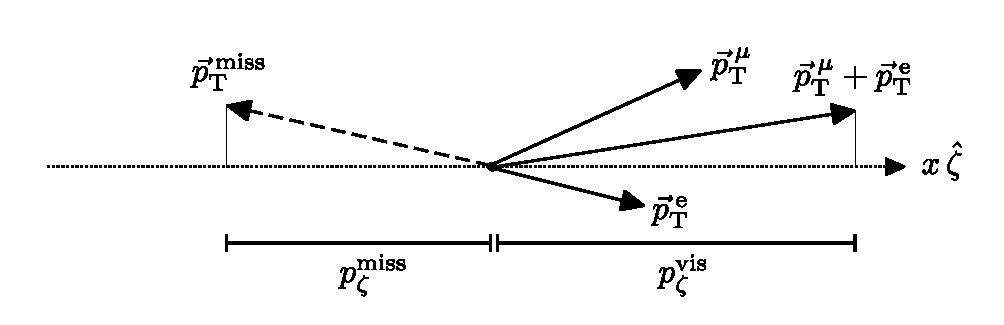
\includegraphics[width=1.0\textwidth]{Figures/dzeta_diagram.pdf}
\caption[Diagram of the inputs to the $D_\zeta$ variable.]{Diagram of the inputs to the $D_\zeta$ variable~\cite{CMS:2022rbd}.}
\label{fig:dzeta_diagram}
\end{figure}

The linear combination is optimised for genuine di-$\tau$ events to peak around $D_{\zeta} = 0$ GeV. 
It is motivated by the expectation that in di-$\tau$ decays from a resonance, the visible and missing (from $\tau$ neutrinos) momenta are roughly aligned and of similar magnitudes.
In W + jets and $\ttbar$ events, the directions of the visible and missing products are expected to be more randomly distributed and lead to a non-peaking $D_{\zeta}$.
Therefore, only events with $D_\zeta >$ -35 GeV are considered for signal events.
No b tag events failing this cut are vetoed, and events with a b tag also failing this cut are used for a $\ttbar$ control region.

\section{Search optimisation}
\label{sec:search_optimisation}

The optimisation of the signal extraction depends on which of the three scenarios, set out at the beginning of this section, is being searched for.
The components of the optimisation are named the high-mass, low-mass and \ac{SM} Higgs optimisation procedures.
For the model-independent search (i) the high- or low-mass optimisation procedures are used depending on whether the mass of the resonance is greater or less than 250 GeV.
The search for the \ac{MSSM} Higgs sector (ii) uses the high mass or the \ac{SM} Higgs optimisation procedures depending on whether the reconstructed di-$\tau$ mass is greater or less than 250 GeV.
The presence of more than one neutrino in the event means that it is not possible to fully reconstruct the di-$\tau$ mass directly.
Instead, the likelihood-based \texttt{SVFit} algorithm is used \cite{Bianchini:2014vza}.
Finally, the search for vector leptoquarks (iii) uses only the high-mass optimisation procedure.
The procedures are discussed in detail below. \\

\subsection{High-mass optimisation}
\label{sec:high_mass_optimisation}

The high-mass optimisation procedure follows what was done in Reference~\cite{CMS_MSSM_Tau_2018}.
Each event is initially split into categories depending on whether it has 0 or $\geq$1 b tagged jets.
Firstly, this helps target the additional Higgs boson production modes gluon fusion and b-associated production respectively.
In particular, bb$\phi$ has final state b quarks that if tagged can significantly aid the sensitivity to this signal.
Secondly, the production of the dominant initial state b quarks for a t-channel vector leptoquark signal can lead to additional b jets in the final state.
The reduced backgrounds in b-tagged events allow for a more sensitive vector leptoquark search in this category. \\

The $\etauh$ and $\mutauh$ channels are further subdivided into categories depending on the transverse mass between the light lepton and missing transverse momentum vectors as defined in Equation~\ref{eqn:mt}.
The corresponding categories are defined as:
\begin{itemize}
\item \texttt{Tight-$m_{\text{T}}$}: $m_{\text{T}}(\pTvec^{\hspace{2pt}e/\mu},\pTvec^{\hspace{2pt}\text{miss}}) < 40$ GeV;
\item \texttt{Loose-$m_{\text{T}}$}: $40 \leq m_{\text{T}}(\pTvec^{\hspace{2pt}e/\mu},\pTvec^{\hspace{2pt}\text{miss}}) < 70$ GeV.
\end{itemize}
The majority of the signal events fall within the \texttt{Tight-$m_{\text{T}}$} sub-category.
The \texttt{Loose-$m_{\text{T}}$} category is used to improve the signal acceptance for resonant masses of $m_{\phi} > 700$ GeV.\\

The $\emu$ channel is subdivided into three signal categories based on the cuts on the variable $D_{\zeta}$ as defined in Equation~\ref{eqn:Dzeta_def}.
The three categories are defined as:
\begin{itemize}
\item \texttt{Low-$D_\zeta$}: $-35 \leq D_\zeta < -10$ GeV;
\item \texttt{Medium-$D_\zeta$}: $-10 \leq D_\zeta <  30$ GeV;
\item \texttt{High-$D_\zeta$}: $D_\zeta \geq 30$ GeV.
\end{itemize}
By design, the majority of signal events are located in the \texttt{Medium-$D_\zeta$} sub-category.
The \texttt{Low-} and \texttt{High-$D_\zeta$} categories are used to catch the tail of the signal distributions.
A schematic of all high-mass optimisation categories is shown in Figure~\ref{fig:high_mass_categories}. \\

\begin{figure}[!hbtp]
\centering
    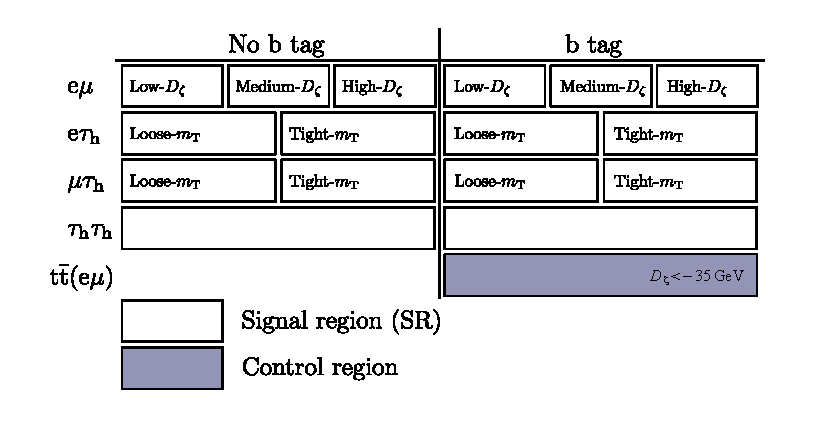
\includegraphics[width=0.85\textwidth]{Figures/high_mass_categories.pdf}
\caption[Diagram of the categories in the high-mass optimisation procedure.]{Overview of the categories used for the extraction of the signal in the high-mass optimisation procedure~\cite{CMS:2022rbd}.}
\label{fig:high_mass_categories}
\end{figure}

Once all category divisions have been applied, events are drawn in histograms based on a discriminating variable.
The discriminating variable used in this analysis is $m_{T}^{\text{tot}}$ and is defined below. \\
\begin{equation}
m_{T}^\text{tot} = \sqrt{m_{T}(\pTvec^{\hspace{2pt}\tau_1},\pTvec^{\hspace{2pt}\text{miss}})^2 +  m_{T}(\pTvec^{\hspace{2pt}\tau_2},\pTvec^{\hspace{2pt}\text{miss}})^2 + m_{T}(\pTvec^{\hspace{2pt}\tau_1},\pTvec^{\hspace{2pt}\tau_2})^2},
\label{eqn:mt_tot}
\end{equation} \\
where $\tau_1$ and $\tau_2$ refer to the visible products of the two $\tau$ lepton decays.
This variable provides excellent discriminating power between higher mass resonant signals compared to other non-peaking backgrounds, whilst still maintaining some separation between signal masses.
It is also excellent at separating the high-mass non-resonant di-$\tau$ signatures from backgrounds, where a di-$\tau$ mass does not represent the mass of a resonance.
This is due to the use of the transverse momenta and \ac{MET} in the variable definition.
For a t-channel signal where the mediator has high mass, no significant mass separation is expected in any variable. \\

\subsection{Low-mass optimisation}

The low-mass optimisation procedure, loosely follows the high-mass procedure with a few key differences.
Categories that are only sensitive to high-mass signals are dropped.
This includes the \texttt{Low-$D_\zeta$} and \texttt{Loose-$m_{T}$} categories.
Each no b tag subcategory is further divided into four bins of reconstructed di-$\tau$ visible $\pT$ with bin edges: 0, 50, 100, 200 and $\infty$.
This is not done in the b tag subcategories due to the lack of statistics in this region.
A schematic of the categories used in the low-mass optimisation procedure is shown in Figure~\ref{fig:low_mass_categories}.
The final difference with the high-mass optimisation procedure is the discriminator used.
In the low-mass optimisation procedure the reconstructed di-$\tau$ mass is used.
This helps to separate signal events from the Z boson peak in this region. \\

\subsection{Standard Model Higgs boson optimisation}

Finally, the \ac{SM} Higgs optimisation procedure is taken from the \ac{CMS} \ac{SM} $H \rightarrow \tau\tau$ analysis and is detailed in Reference~\cite{CMS:2022kdi}.
This was previously used for simplified template cross-section measurements.
This uses a \ac{NN}-based categorisation to obtain the most precise estimates from data of the \ac{SM} Higgs produced via gluon fusion, vector boson fusion or vector boson-associated production.
The \ac{NN} based analysis introduces 26 categories, 8 of which are optimised to pull out the Higgs boson signal.
Although the \ac{NN} is trained specifically to target events with an \ac{SM}-like Higgs boson, signal events with differing masses can also enter the \ac{NN} categories.

\begin{figure}[!hbtp]
\centering
    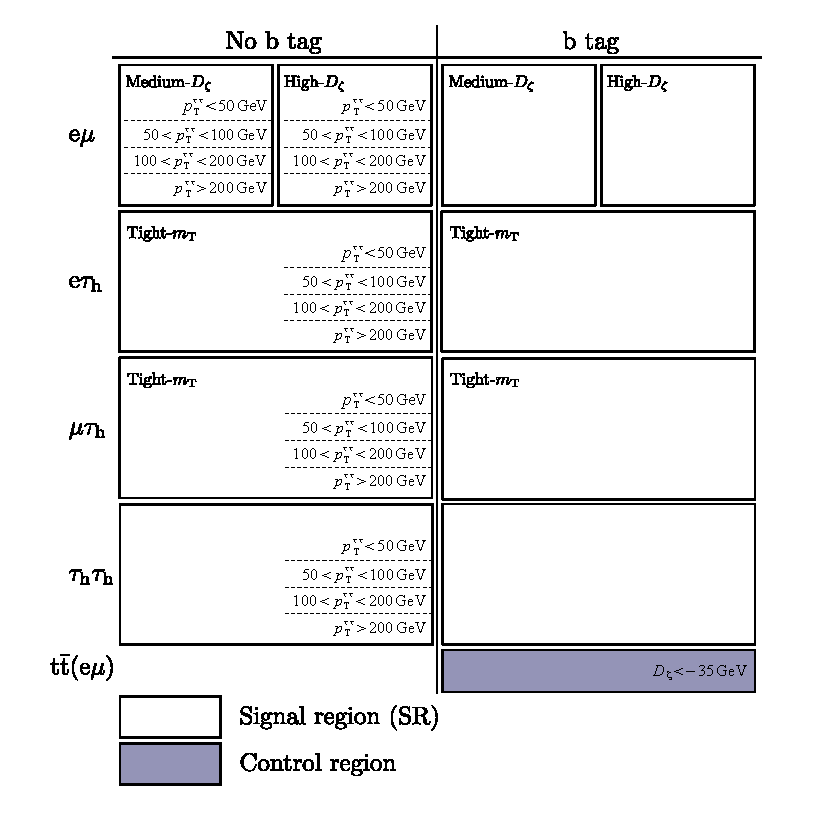
\includegraphics[width=0.85\textwidth]{Figures/low_mass_categories.pdf}
\caption[Diagram of the categories in the low-mass optimisation procedure.]{Overview of the categories used for the extraction of the signal in the low mass optimisation procedure~\cite{CMS:2022rbd}.}
\label{fig:low_mass_categories}
\end{figure}

\section{Background modelling overview}
\label{sec:background_modelling}

The relevant backgrounds for this analysis include $Z/\gamma^*$, $\ttbar$, W+jets, \ac{QCD}, di-boson, single-top, and electroweak W and Z bosons production.
These are split into five categories:
\begin{enumerate}[i)]
  \item Events containing only genuine $\tau$ leptons.
  \item Events with a jet misidentified as a $\tau_h$ (\jtth) in the $\etauh$, $\mutauh$ or $\tauhtauh$ channels.
  \item Events with jets misidentified as both light leptons ($\text{jet}\rightarrow \ell$) in the $\emu$ channel.
  \item Events from $\ttbar$ with a prompt light lepton ($e$ or $\mu$ not from a $\tau$ decay) and the other object (if there are not two prompt light lepton) is from a genuine $\tau$ lepton.
  \item Other events. This is a small contribution and so it is grouped.
  \begin{itemize}
    \item Non $\ttbar$ events satisfying (iv).
    \item Events with a light lepton misidentified as a $\tau_h$ and no \jtth candidate. 
    \item Events with a jet misidentified as a light lepton and the other object is from genuine $\tau$ leptons in the $\etauh$, $\mutauh$ or $\tauhtauh$ channels.
    \item Events with a muon misidentified as an electron in the $\emu$ channel.
    \item Events with one jet misidentified as a light lepton and the other object from a prompt light lepton in the $\emu$ channel.
   \end{itemize}
\end{enumerate}

Backgrounds from (i) consist of largely Z/$\gamma^* \rightarrow \tau\tau$ events but there are also smaller contributions from other processes. 
This background is modelled by a data-simulation hybrid method called the \say{embedding} method~\cite{CMS_embedding} and this is described in detail in Section~\ref{sec:embedding}.
Group (ii) is dominated by \ac{QCD}, W + jets and $\ttbar$ events with a \jtth misidentification.
This is modelled from data by the \say{fake factor} ($\FF$) method~\cite{Sirunyan:2018zut,CMS:2018lkr} and is explained in Section~\ref{sec:ff}.
Group (iii) is modelled from data to describe the \ac{QCD} multijet contribution to the background in the $\emu$ channel.
The method to obtain this background is described in Section~\ref{sec:qcd}.
The data-driven background estimations for (i), (ii) and (iii) contribute $\approx$98\% of all expected background events in the $\tauhtauh$ channel, $\approx$90\% in $\etauh$ and $\mutauh$ channels and $\approx$50\% in the $\emu$ channel.
The final groups, (iv) and (v), are modelled with \ac{MC} simulations.
The $\ttbar$ process from (iv) is separated because of its large contribution to the phase space where a b jet is required. \\

In 2016 (2017--2018), the W + jets and $Z\rightarrow \ell\ell$ processes are simulated using the \MGvATNLO 2.2.2 (2.4.2) event generator at \ac{LO}~\cite{Alwall:2011uj}. 
Supplementary samples are generated with up to four outgoing partons in the hard interaction to increase the number of simulated events in regions of high signal purity. 
For di-boson production, \MGvATNLO is used at \ac{NLO} precision~\cite{Alwall:2011uj}, and the FxFx~\cite{Frederix:2012ps} (MLM~\cite{Alwall:2007fs}) prescription is used to match the \ac{NLO} (\ac{LO}) matrix element calculation with the parton shower model. 
Samples for $\ttbar$~\cite{Alioli:2011as} and (t-channel) single top quark production~\cite{Frederix:2012dh} are generated at \ac{NLO} precision using \POWHEG 2.0~\cite{Nason:2004rx,Frixione:2007vw,Alioli:2010xd,Jezo:2015aia}, and for single top quark production in association with a W boson (tW channel)~\cite{Re:2010bp}, \POWHEG version 1.0 at \ac{NLO} precision is used. 
When compared with data, W + jets, $Z\rightarrow \ell\ell$, $\ttbar$, and single top quark events in the tW channel are normalised to their cross-sections at \ac{NNLO} precision\cite{Melnikov:2006kv,Czakon:2011xx,Kidonakis:2013zqa}, while single top quark and di-boson events are normalised to their cross-sections at \ac{NLO} precision or higher~\cite{Kidonakis:2013zqa,Campbell:2011bn,Gehrmann:2014fva}.

\section{QCD estimation in the $\emu$ channel}
\label{sec:qcd}

The \ac{QCD} model in the $\emu$ channel, which attempts to model events where two jets are misidentified as an electron-muon pair, is taken from data where the electron and muon have the same sign, with a transfer factor ($F_{T}$).
The transfer factor determines differences from the same sign to opposite sign region and is calculated from a sideband region with an anti-isolated muon ($0.2 < \Irel < 0.5$).
$F_{T}$ is initially parametrised by the $\Delta R$ between the electron and muon, and the number of jets in the event 
However, additional dependencies on the electron and muon $\pT$ enter via a correction. \\

Good agreement is observed in events with no b jets when applying $F_{T}$ onto same sign events compared to opposite sign events where both regions have an anti-isolated muon. 
However, in events with a b jet, an additional correction is needed.
This is determined to be $\approx$0.75 (differs very slightly between data-taking years).
As this correction is large, it is validated by switching the light lepton anti-isolation so that the election is required to have $0.15 < \Irel < 0.5$.
Also, events where both light leptons are anti-isolated are looked at.
The correction for b-tagged events is equivalent in all three regions, and a global average of the three is taken for the final correction. \\

To understand the physical reason for the large difference in no b tag and b tag events in same sign and opposite pairs, studies were performed on simulated samples.
It was observed that the electron-muon pair is usually produced from pairs of heavy quarks, $pp\rightarrow b\bar{b}$ ($c\bar{c}$).
If the two jets are initiated from the heavy quarks there is a large bias towards opposite sign jets due to the opposite signs of the quark-antiquark pair.
However, if one of the heavy quarks is tagged as a b jet, another object has to be the jet initiator (a radiated gluon for example) and there is therefore no charge preference in the pair.
As $F_{T}$ is originally fit inclusively in numbers of b jets and the 0 bin is dominant, the correction overpredicts the opposite sign to same sign ratio and so a large correction is needed as observed.

\section{Embedding method}
\label{sec:embedding}

The background for genuine di-$\tau$ lepton pairs is modelled via the embedding method~\cite{CMS_embedding}. 
This is a hybrid method that utilises both data and \ac{MC} techniques to produce high-statistic samples, where the bulk of the event comes from data.
This minimises both the chance of \ac{MC} fluctuations and the size of the uncertainties.
The genuine di-$\tau$ background is dominated by the $Z \rightarrow \tau \tau$ process, but there will be smaller contributions from $t\bar{t}$ and di-boson processes.  \\

The algorithm first selects $\mu\mu$ events from data.
The selection is chosen to naturally target the pure $Z \rightarrow \mu\mu$ region but still be loose enough to catch events from other processes, so as not to introduce a bias on the Z boson mass.
Events are required to pass the double-$\mu$ trigger with minimum requirements on the invariant mass of the two muons ($m_{\mu\mu}$) and the $\pT$ of the leading and trailing muons.
Also required at the trigger level is a loose association of the track to the \ac{PV} and a loose isolation in the tracker.
Offline objects matched to the trigger muons, are then required to have standard $d_z$ and $\eta$ selections and originate from a global muon track, as defined in Section~\ref{sec:object_reconstruction}.
The muon pair are required to have an opposite charge and have $m_{\mu\mu} > 20$ GeV.
The fraction of processes within this selection is tested with \ac{MC} background samples and a \ac{QCD} model from same sign muon pairs with an extrapolation factor.
Approximately 97\% of selected events are expected to come from $Z/\gamma^* \rightarrow \mu\mu$ events with smaller contributions from $Z/\gamma^* \rightarrow \tau\tau$ ($\tau\rightarrow\mu$), di-boson, $\ttbar$ and QCD.
The di-boson and $\ttbar$ relative contributions are greater at higher $m_{\mu\mu}$ and in events with tagged b jets, whilst the \ac{QCD} contribution is largest at lower $m_{\mu\mu}$.
The events selected are biased by detector acceptances. 
Therefore, corrections on the reconstruction and identification efficiencies are performed in muon $\eta$ and $\pT$ using the \say{tag-and-probe} method, as described in Reference~\cite{CMS:2010svw}. \\

Next, all energy deposits in the detector from the selected muons are removed.
This involves removing the hits on global muon tracks in the tracker, hits in the muon systems and clusters in the calorimeters that intercept the muon trajectory.
Once completed, the selected muons and their kinematic properties are replaced with simulated $\tau$ leptons.
To account for the difference in mass between the muon and $\tau$, the muons are boosted into the centre-of-mass frame of the di-muon system and then this four-vector is taken for the $\tau$ but boosted back into the laboratory frame.
The event simulation is performed from the \ac{PV}.
The $\tau$ lepton decay is then simulated with \PYTHIA~\cite{Sirunyan:2019dfx,Sjostrand:2014zea} and separate samples are produced for different $\tau\tau$ decay channels.
Only the decay of the $\tau$ leptons is then processed through the detector simulation and the remainder of the $\mu\mu$ event is added back.
A schematic of the process is shown in Figure~\ref{fig:embedding}. \\

\begin{figure}[!hbtp]
\centering
    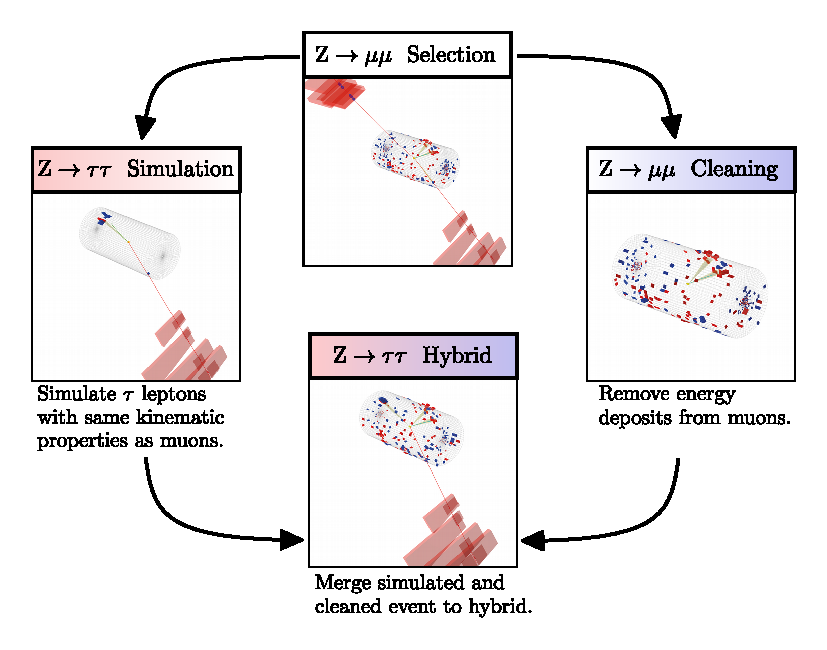
\includegraphics[width=0.9\textwidth]{Figures/Embedding_Diagram.pdf}
\caption[Diagram of the embedding method.]{Schematic of the embedding method to model genuine di-$\tau$ backgrounds from di-muon events in data~\cite{CMS_embedding}.}
\label{fig:embedding}
\end{figure}

The embedding method is validated on dedicated samples, where the muons from data are replaced by simulated muons instead of $\tau$ leptons.
A plot of the agreement from these dedicated samples with data is shown in Figure~\ref{fig:emb_validation}.

\begin{figure}[!hbtp]
\centering
    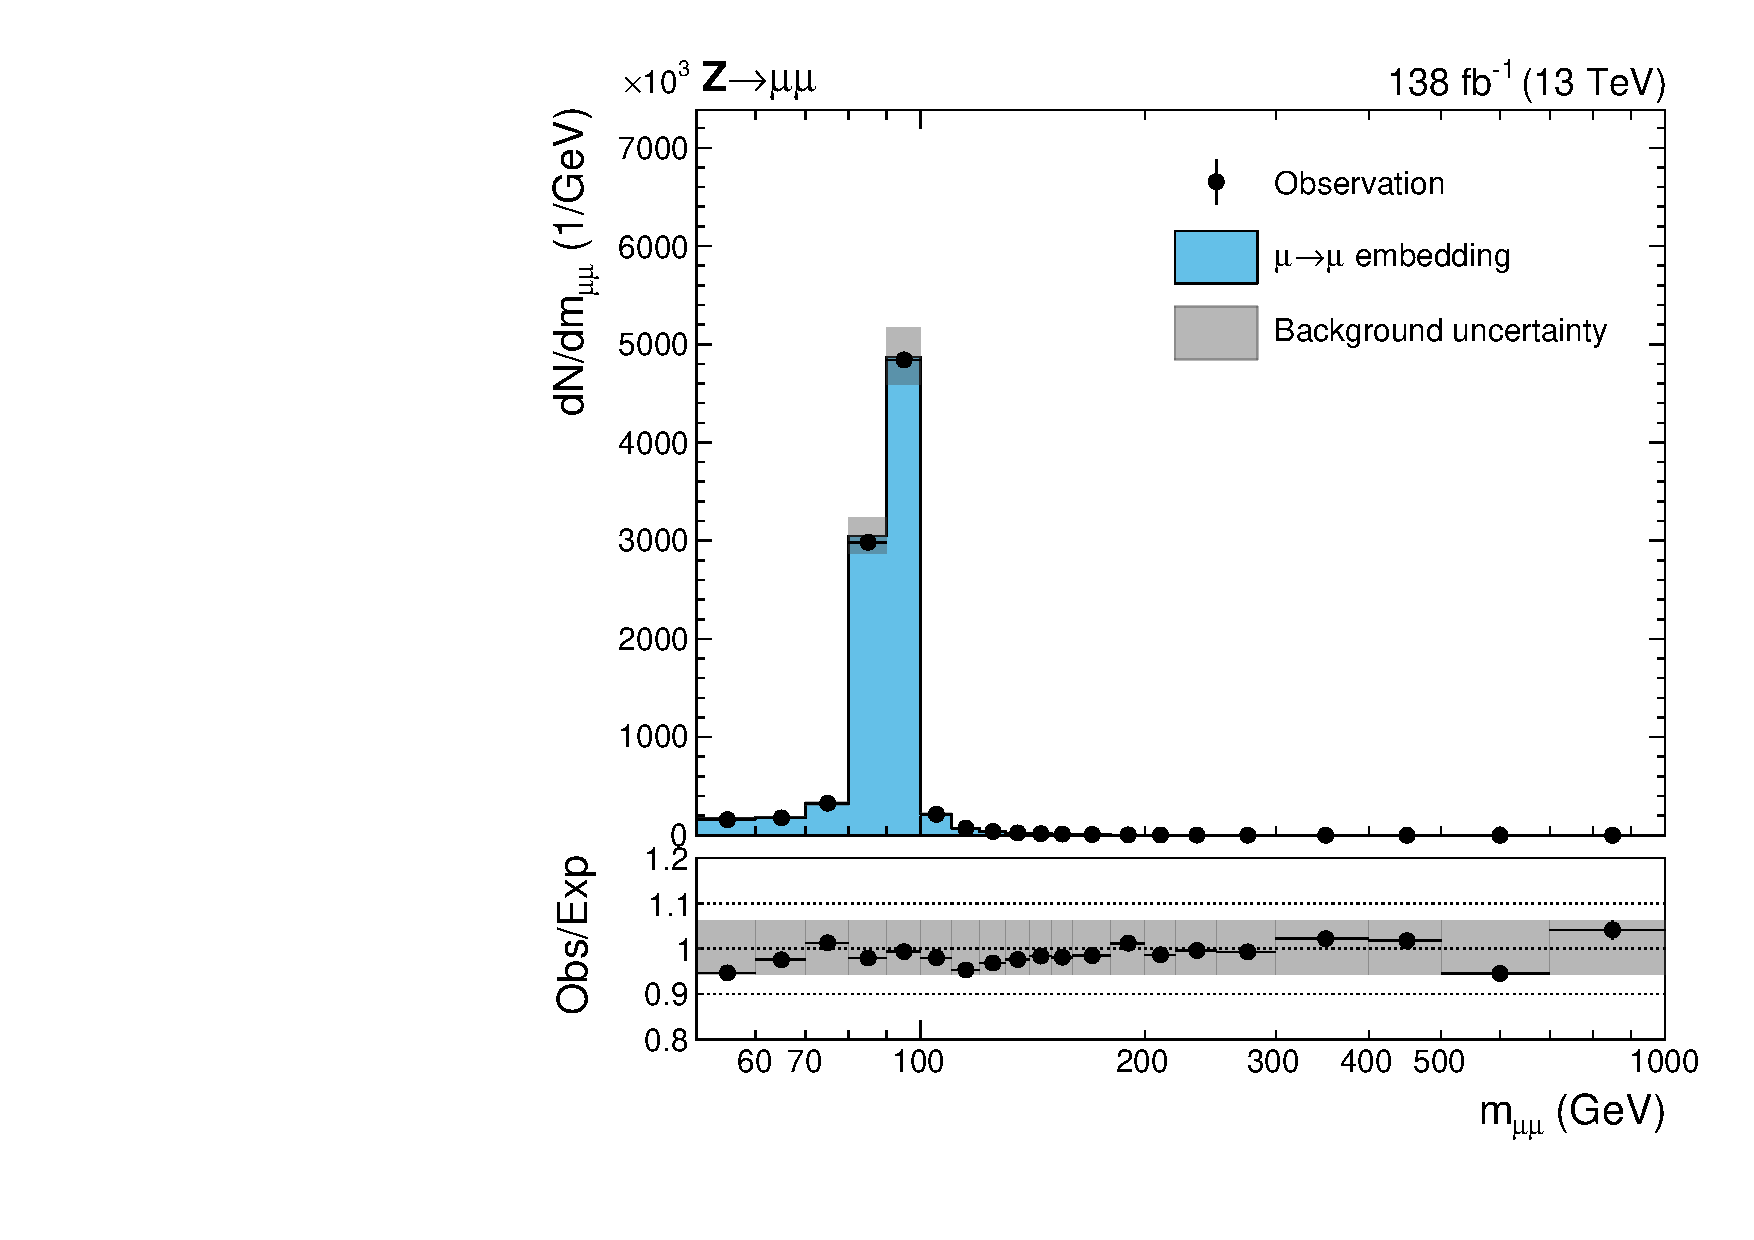
\includegraphics[width=0.7\textwidth]{Figures/embedding_validation.pdf}
\caption[Plot of the validation of the embedding method.]{Closure plot showing the di-muon mass on the dedicated embedding validation samples.}
\label{fig:emb_validation}
\end{figure}

\section{Fake factor method}
\label{sec:ff}

Backgrounds in which a jet is misidentified as a $\tauh$ can be difficult to model using \ac{MC} due to the poor description of the \jtth fake rate in simulation. 
In addition, the small probability of a jet being misidentified as a $\tauh$ necessitates the production of high statistics \ac{MC} samples at a significant computational expense.
These shortcomings motivate the use of data-driven estimations for these processes. 
One such procedure is the $\FF$ method~\cite{Sirunyan:2018zut,CMS:2018lkr}. \\

The $\FF$ method utilises regions in the data to model the \jtth background. 
Firstly, the determination regions are defined, which are \jtth enriched regions orthogonal to the signal region. 
They are then purified by subtracting off any non \jtth events with \ac{MC}.
It is used to calculate a $\FF$ by taking the ratio of the number of \jtth events that pass the nominal $\tau_h$ identification requirement ($N(\texttt{Nominal})$), to the number of \jtth events that fail the nominal $\tau_h$ identification but pass a looser alternative $\tau_h$ identification requirement ($N(\texttt{Alternative}\text{ and not }\texttt{Nominal})$), as shown in Equation~\ref{eqn:ff}.

\begin{equation}
\FF = \frac{N(\texttt{Nominal})}{N(\texttt{Alternative}\text{ and not }\texttt{Nominal})}.
\label{eqn:ff}
\end{equation}

In the remaining text, this numerator and denominator are referred to as the pass and fail regions.
The derivation of this ratio is done differentially with respect to key parameters that differ in the two regions.
Once $\FF$ have been derived it is common to calculate corrections in other sideband regions and combine $\FF$ measured from different processes.
Finally, the $\FF$ are applied to the application region. 
This is defined as the signal region but with the criteria that the \jtth events fail the nominal $\tau_h$ identification but pass the looser alternative $\tau_h$ identification requirement.
This now models the background from \jtth events in the signal region. \\

The following Sections~\ref{sec:ff_dr}--\ref{sec:ff_applying} detail the complexities of how this method is applied to this analysis.
For these searches, the nominal $\tau_h$ identification used is the \texttt{Medium} $D_{\text{jet}}^{\text{WP}}$ and the alternative $\tau_h$ identification used is the \texttt{VVVLoose} $D_{\text{jet}}^{\text{WP}}$.

\subsection{Determination regions}
\label{sec:ff_dr}

The $\FF$ are measured separately in each year of data taking period (2016, 2017, 2018), in each channel containing a $\tau_h$ ($\etauh$, $\mutauh$, $\tauhtauh$) and in enriched regions of dominant processes that contribute \jtth events.
In the $\etauh$ and $\mutauh$ channels $\FF$ are measured for three processes: \ac{QCD}, W + jets and $\ttbar$.
In the $\tauhtauh$ channel $\FF$ are measured only for the dominant \ac{QCD} process.
The \ac{QCD} process is assumed to produce two jets misidentified as $\tauh$ candidates, and so the $\FF$ is chosen to be calculated from leading $\pT$ $\tau_h$ candidate only.
Section~\ref{sec:ff_applying} discusses how a single \jtth events in the $\tauhtauh$ channel are modelled. \\

Each separate measurement region is split into three sideband regions based on two cuts that surround the signal region.
These regions are named the \texttt{Determination Region} (A), \texttt{Alternative Determination Region} (B) and \texttt{Correction Region} (D) and are schematically shown in Figure~\ref{fig:ff_schematic}. \\

\begin{figure}[!hbtp]
\centering
    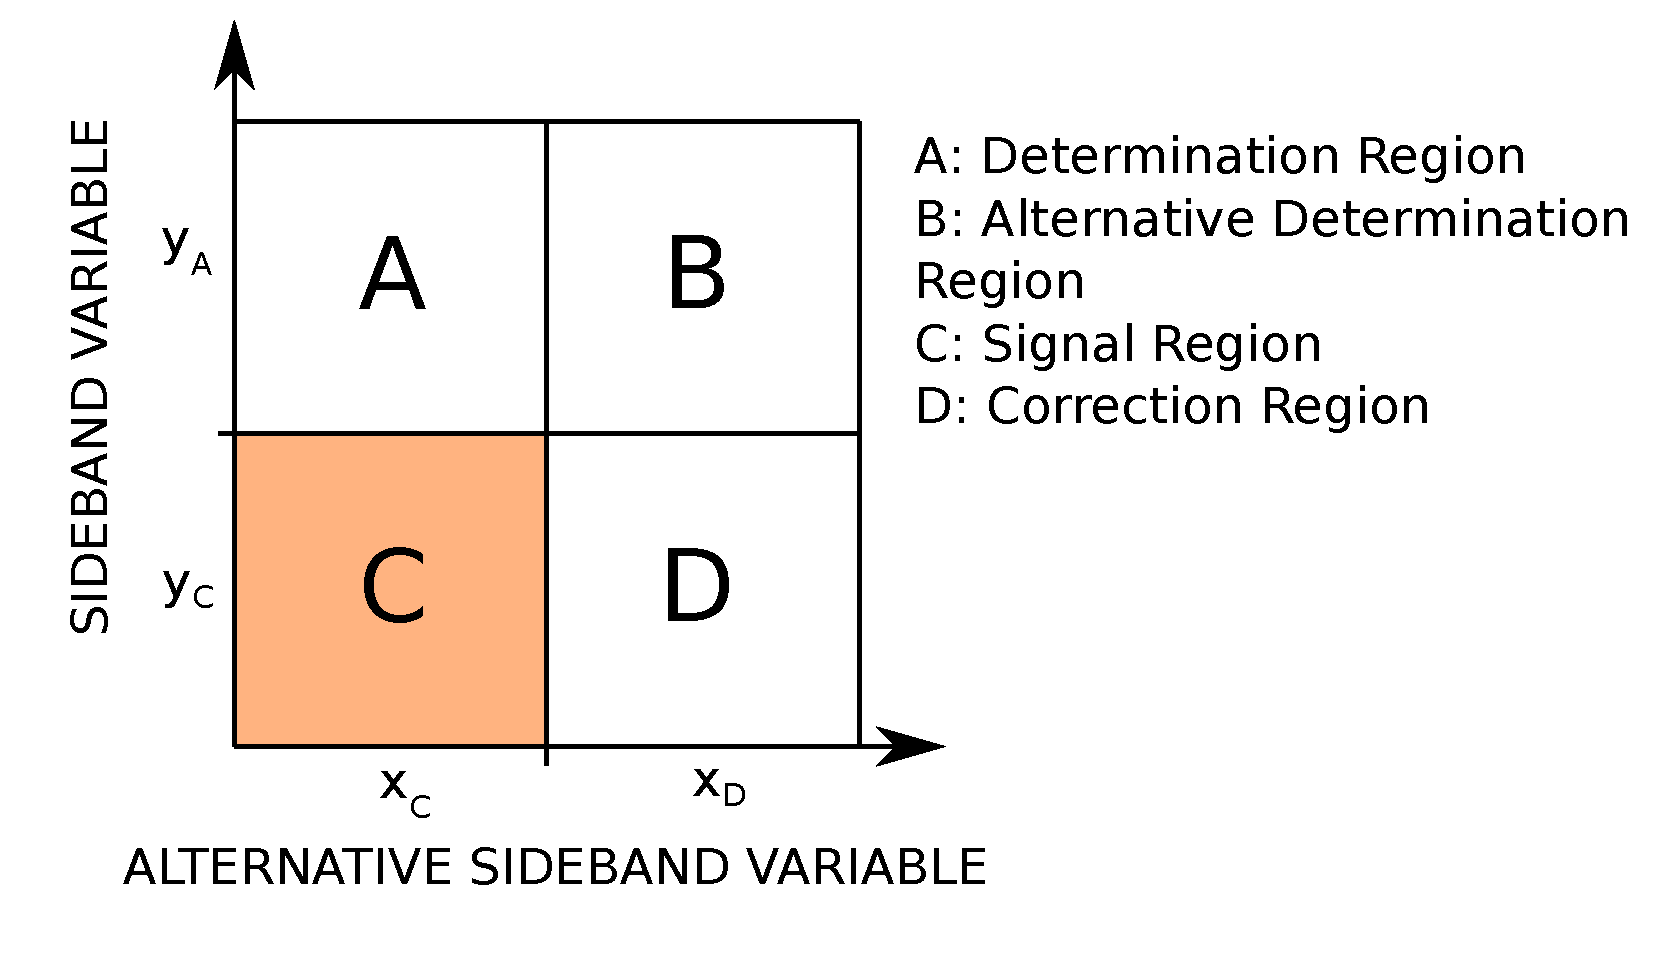
\includegraphics[width=0.8\textwidth]{Figures/ff_diagram_v2.pdf}
\caption[Diagram of the regions used for fake factor derivation.]{Schematic of the regions used for fake factor derivation.}
\label{fig:ff_schematic}
\end{figure}

Region A is used to measure and fit the $\FF$.
Region B is an alternative region used to measure and fit the $\FF$ to account for the difference between A and C.
These alternative $\FF$ are applied to the fail $\tauh$ identification region in D and corrections are calculated by comparing it to the pass region in D.
The total $\FF$ per measurement region is calculated as the product of the $\FF$ derived in region A and the correction calculated from region B to D. \\

The selection for $x_C$, $x_D$, $y_C$ and $y_A$, as defined in Figure~\ref{fig:ff_schematic}, in each separate measurement region are shown below.
These are chosen to balance the number of events and the purity of each background in the region.

\begin{enumerate}[i)]
   \item $\tauhtauh$ \ac{QCD} \\
     \indent $y_C$: The $\tauh$ candidates are required to have the opposite sign. \\
     \indent $y_A$: The $\tauh$ candidates are required to have the same sign. \\
     \indent $x_C$: The subleading $\tau_h$ passes the \texttt{Medium} $D_{\text{jet}}^{\text{WP}}$. \\
     \indent $x_D$: The subleading $\tau_h$ fails the \texttt{VVLoose} $D_{\text{jet}}^{\text{WP}}$ but passes the \texttt{VVVLoose} $D_{\text{jet}}^{\text{WP}}$.
  \item $\etauh$ and $\mutauh$ \ac{QCD} \\
    \indent $y_C$: The $e$/$\mu$ and $\tauh$ candidates are required to have the opposite sign. \\
    \indent $y_A$: The $e$/$\mu$ and $\tauh$ candidates are required to have the same sign and the $e$/$\mu$ to have $\Irel>0.05$. \\
    \indent $x_C$: The $e$/$\mu$ candidate is required to have $\Irel<0.15$. \\
    \indent $x_D$: The $e$/$\mu$ candidate is required to have $0.25<\Irel<0.5$.
  \item $\etauh$ and $\mutauh$ W + Jets \\
    \indent $y_C$: The $\mT$ between the $e$/$\mu$ and the \ac{MET} $< 70$ GeV. \\
    \indent $y_A$: The $\mT$ between the $e$/$\mu$ and the \ac{MET} $> 70$ GeV and no b jets in the event. \\
    \indent $x_C$: Data. \\
    \indent $x_D$: W + Jets \ac{MC}.
  \item $\etauh$ and $\mutauh$ $\ttbar$ \\
    \indent $y_C$: Data. \\
    \indent $y_A$: \ac{MC} ($\ttbar$ in B and W + Jets D). \\
    \indent $x_C$: $\mT < 70$ GeV. \\
    \indent $x_D$: $\mT > 70$ GeV and no b jets. \\
\end{enumerate}


In the $\mu\tauh$ and $e\tauh$ channels, W + jets \jtth events are in general the most significant and \ac{QCD} contributes a smaller fraction. 
$\ttbar$ inclusively is small but becomes more significant when searching for events with a b jet. 
The additional $\Irel>0.05$ requirement in these channels for \ac{QCD} is to reduce processes producing genuine leptons and the $N_{\text{b jets}}=0$ requirement for W + Jets is to reduce $\ttbar$ contamination.
It is not possible to define a \texttt{Determination Region} that is sufficiently pure in $\ttbar$ events to make a reasonable measurement of $\FF$ from data.
Therefore, $\ttbar$ $\FF$ are derived from \ac{MC}. 
A comparison of the W + jets $\FF$ measured in data and \ac{MC} shows only $\sim$ 10--20\% differences in the fake rates in data and \ac{MC}.  
This observation coupled with the fact that the $\ttbar$ contribution is small compared to the other processes means that any bias introduced by using $\FF$ measured in \ac{MC} is small compared to the uncertainties on the $\FF$, discussed in Section~\ref{sec:uncerts}. 
In many cases, selections on the regions B and D are applied which are tighter than required, to purify the regions as much as possible, while maintaining enough statistics to perform the fit.\\


\subsection{Parametrisation}
\label{sec:ff_params}

The raw $\FF$ take into account dependencies on $N_{\text{jets}}$ via an analysis-category tailed variable $N_{\text{pre b jets}}$, the $\pT$ of the $\tauh$ candidate ($\pT^{\tauh}$) and the $\pT$ of the jet that seeds the \ac{HPS} algorithm ($\pT^{\text{jet}}$).
$N_{\text{pre b jets}}$ is the number of jets in the event with $|\eta|<2.4$ and $\pT>20$ GeV, which is the $\eta$ and $\pT$ selection for a b-tagged jet. 
It is defined to map the dependence of $\FF$ on the number of jets and describe the categorising variable $N_{\text{b jets}}$ well.
Although not local to the $\tauh$, it helps control other dependencies on the constituents of the event.
It is the number of jets in the event with $|\eta|<2.4$ and $\pT>20$ GeV. 
These are the same $\eta$ and $\pT$ thresholds required for a b jet.
The data is split into two bins of $N_{\text{pre b jets}}$, equal to 0 and greater than 0.
It is then further split by the ratio of $\pT^{\text{jet}}$ to $\pT^{\tauh}$.
An example of the dependence of these two transverse momentums on the fake factor is shown in Figure~\ref{fig:ff_colz}. \\

\begin{figure}[!hbtp]
\centering
    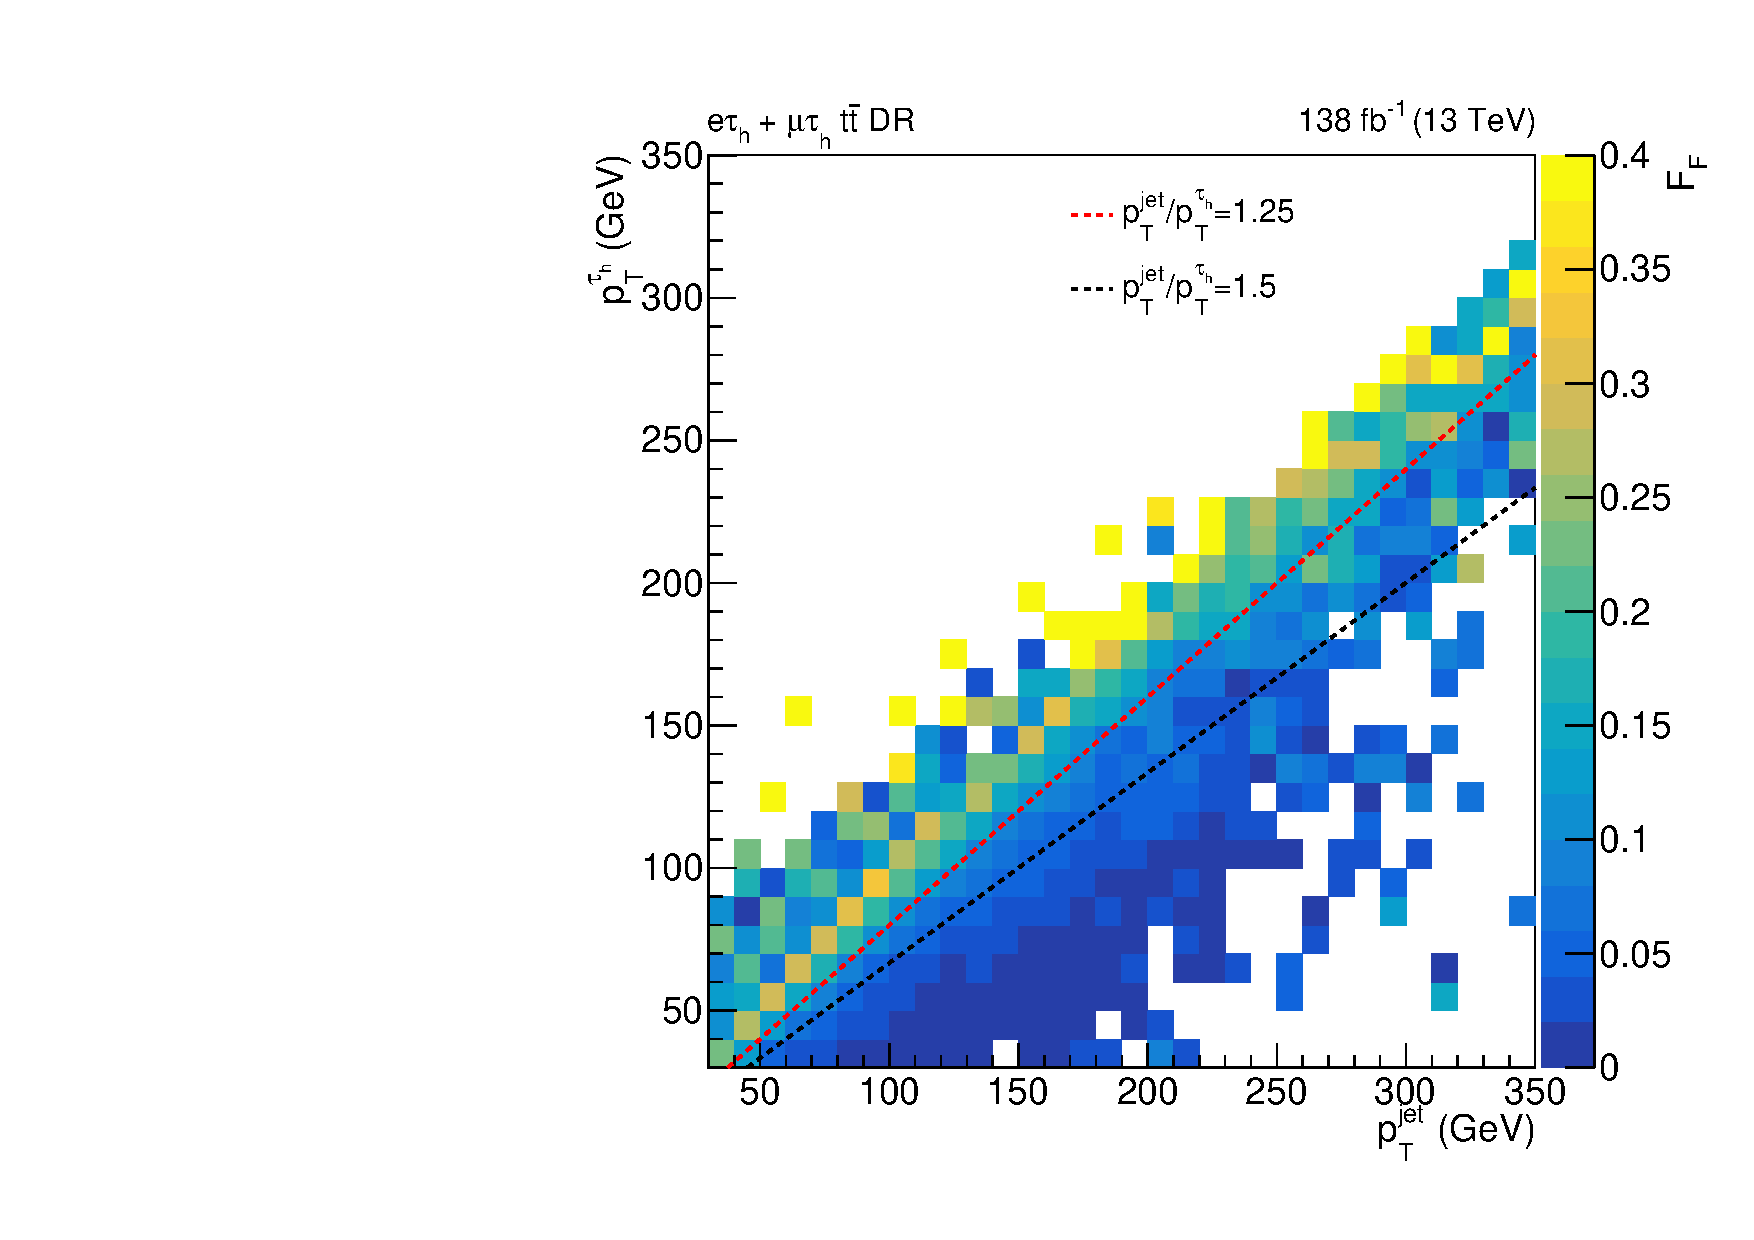
\includegraphics[width=0.6\textwidth]{Figures/ff_colz_ttbar_lt_v2.pdf}
\caption[Plot of the reliance of the fake factors on the ratio of the $\tauh$ and jet $\pT$.]{A 2D heat map of the $\FF$ determined from $t\bar{t}$ MC for the full Run 2 dataset in the combined $e\tauh$ and $\mu\tauh$ channels. This is shown with respect to the $\tau_h$ $\pT$ and the $\pT$ of the HPS seeded jet for the $\tauh$. The ratio of jet to $\tau_h$ $\pT$ categorisation used is shown split by the dashed lines.}
\label{fig:ff_colz}
\end{figure}

It is motivated by the observation that the $\FF$ are largest when the $\pT^{\text{jet}}$ and $\pT^{\tauh}$ are closest.
The physical motivation for this is when they are close, the $\tauh$ candidate is likely to be isolated from any other hadronic activity and so more likely to be identified as a $\tau$.
However, when $\pT^{\text{jet}}$ is larger than $\pT^{\tauh}$, the candidate is likely surrounded by other hadronic activity and so more likely to be a jet fake.
When $\pT^{\text{jet}}$ is less than $\pT^{\tauh}$, charged pions are likely not close enough to the \ac{PV} to be clustered into the jet and so the event is less likely to be classified as a $\tauh$. 
This leads to the $\FF$ dependence as seen in Figure~\ref{fig:ff_colz}.\\

For all divisions of the phase space, dependence on the $\pT^{\tauh}$ is fit using the superposition of a Landau function and a constant in the low-$\pT$ region.
The $\FF$ are seen to rise sharply at high $\pT$.
This increase happens in either the bin 140 $<$ $\pT^{\tauh}$ $<$ 200 GeV or $\pT^{\tauh}$ $>$ 200 GeV.
To map this effect, binned values are taken based on the algorithm shown in Figure~\ref{fig:ff_binning} and the fit is used below the minimum bin.

\begin{figure}[!hbtp]
  \centering
  \begin{tikzpicture}[node distance = 8cm, auto]
    % nodes
    \node [block] (start) {Fractional Error in $\pT$ (GeV) Bin, $\frac{\Delta N}{N}$.};
    \node [decision, aspect=2, node distance=5cm, right of = start] (d1) {[140,200)};
    \node [decision, aspect=2, node distance=3cm, above of = d1] (d2) {[200,$\infty$)};
    \node [decision, aspect=2, node distance=3cm, below of = d1] (d3) {[200,$\infty$)};
    \node [block3, aspect=2, node distance=3cm, above of = d2] (n1) {Use bin values in [140,200,$\infty$)};
    \node [block3, aspect=2, node distance=3cm, below of = d3] (n2) {Use bin values in [200,$\infty$)};
    \node [block3, aspect=2, node distance=5cm, right of = d2] (n3) {Use bin values in [140,$\infty$)};
    \node [block3, aspect=2, node distance=5cm, right of = d3] (n4) {Use no bins};
    % edges
    \draw [arrow] (start) -- (d1);
    \draw [arrow] (d1) -- node[anchor=east] {$>0.5$} (d2);
    \draw [arrow] (d1) -- node[anchor=east] {$<0.5$} (d3);
    \draw [arrow] (d2) -- node[anchor=east] {$>0.5$} (n1);
    \draw [arrow] (d2) -- node[anchor=south] {$<0.5$} (n3);
    \draw [arrow] (d3) -- node[anchor=east] {$>0.5$} (n2);
    \draw [arrow] (d3) -- node[anchor=south] {$<0.5$} (n4);
  \end{tikzpicture}
  \vspace{1cm}
  \caption[Diagram of the algorithm used to choose the binned values taken at high $\pT$ during the fake factor fitting.]{Flow chart of the algorithm used to determine where binned values are taken instead of the fit. The blue box represents the input, the green diamonds represent the decisions and the red boxes represent the outputs.}
  \label{fig:ff_binning}
\end{figure}

The fits are flattened at $\pT^{\tau_h}$ values where there is no significant downward shift or at the final bin to avoid extrapolating past the fitted range. 
$\FF$ fits with respect to $\pT^{\tau_h}$ are shown in Figures~\ref{fig:tt_ff_fit}-\ref{fig:mt_ff_fit}. 
The $\FF$ are highest in the lowest $\pT^{\text{jet}}/\pT^{\tau_h}$ bin and lowest in the highest $\pT^{\text{jet}}/\pT^{\tau_h}$ bin, as expected. 
Otherwise, the $\FF$ fall with $\pT$ in each category until the thresholds used for the high $\pT$ binning algorithm.

\begin{figure}[!hbtp]
\centering
    \subfloat[]{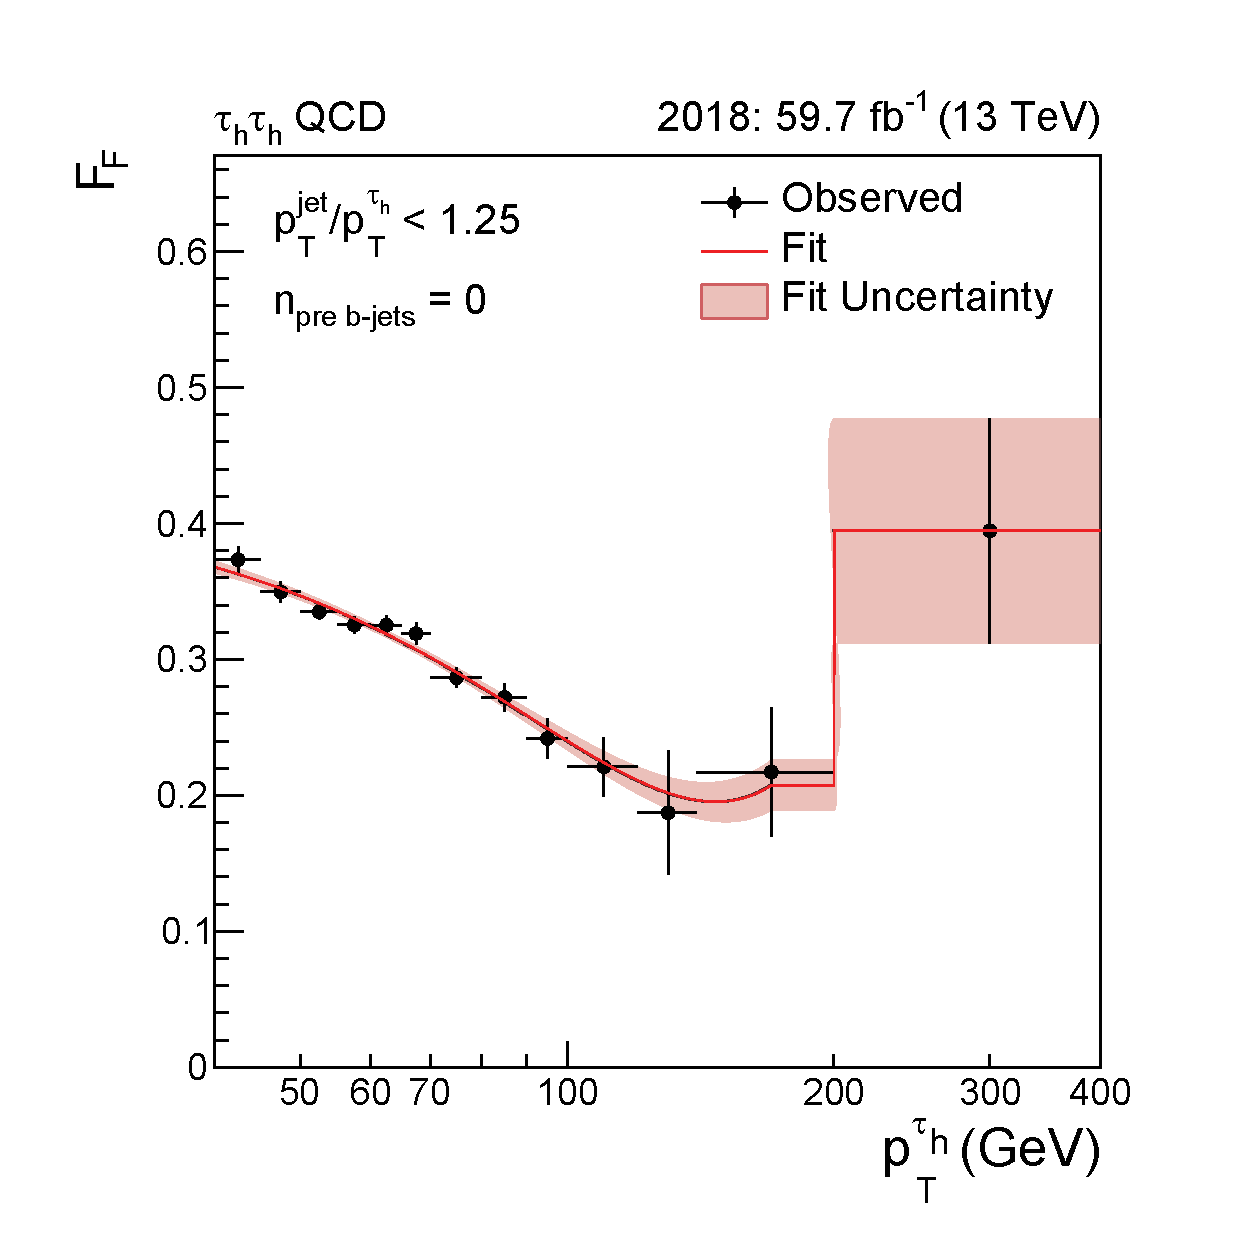
\includegraphics[width=0.33\textwidth]{Figures/ff_fit_jet_pt_low_0jet_pt_1_ff_qcd_tt_2018-EK.pdf}}
    \subfloat[]{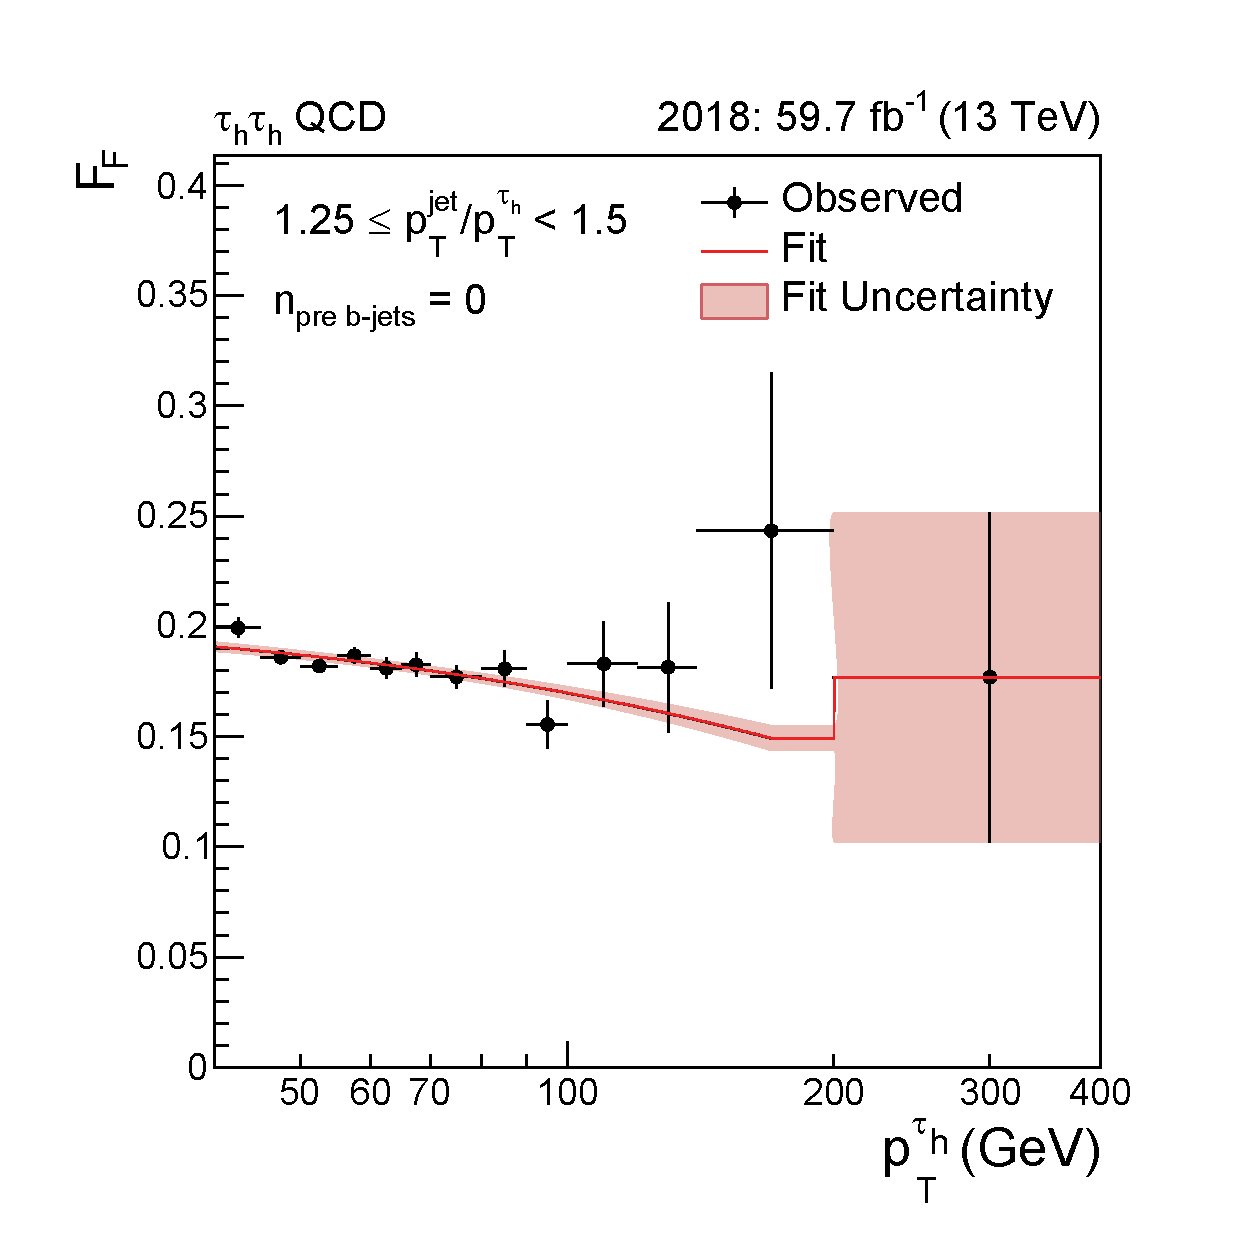
\includegraphics[width=0.33\textwidth]{Figures/ff_fit_jet_pt_med_0jet_pt_1_ff_qcd_tt_2018-EK.pdf}} 
    \subfloat[]{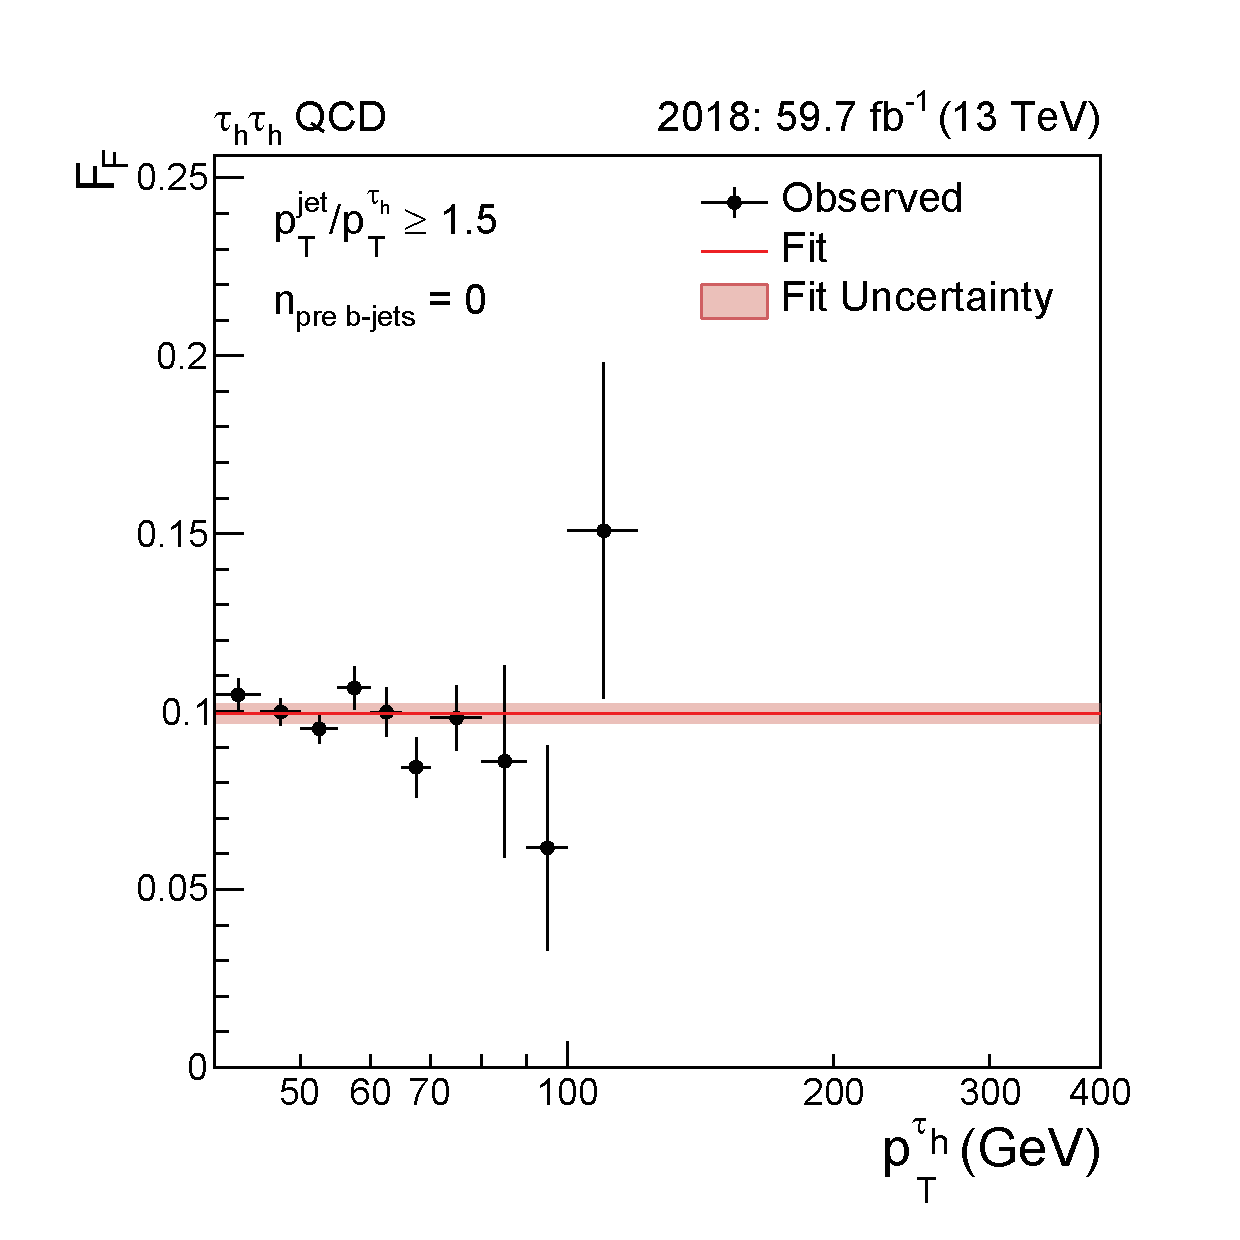
\includegraphics[width=0.33\textwidth]{Figures/ff_fit_jet_pt_high_0jet_pt_1_ff_qcd_tt_2018-EK.pdf}} \\
\caption[Plots of the fake factor fits in the $\tauh\tauh$ channel.]{$\FF$ fits in $\tauh\tauh$ channel for the QCD $N_{\text{pre b jets}}=0$ category with 2018 data. The three jet $\pT$ to $\tau_h$ $\pT$ categories are shown.}
\label{fig:tt_ff_fit}
\end{figure}

\begin{figure}[!hbtp]
\centering
    \subfloat[]{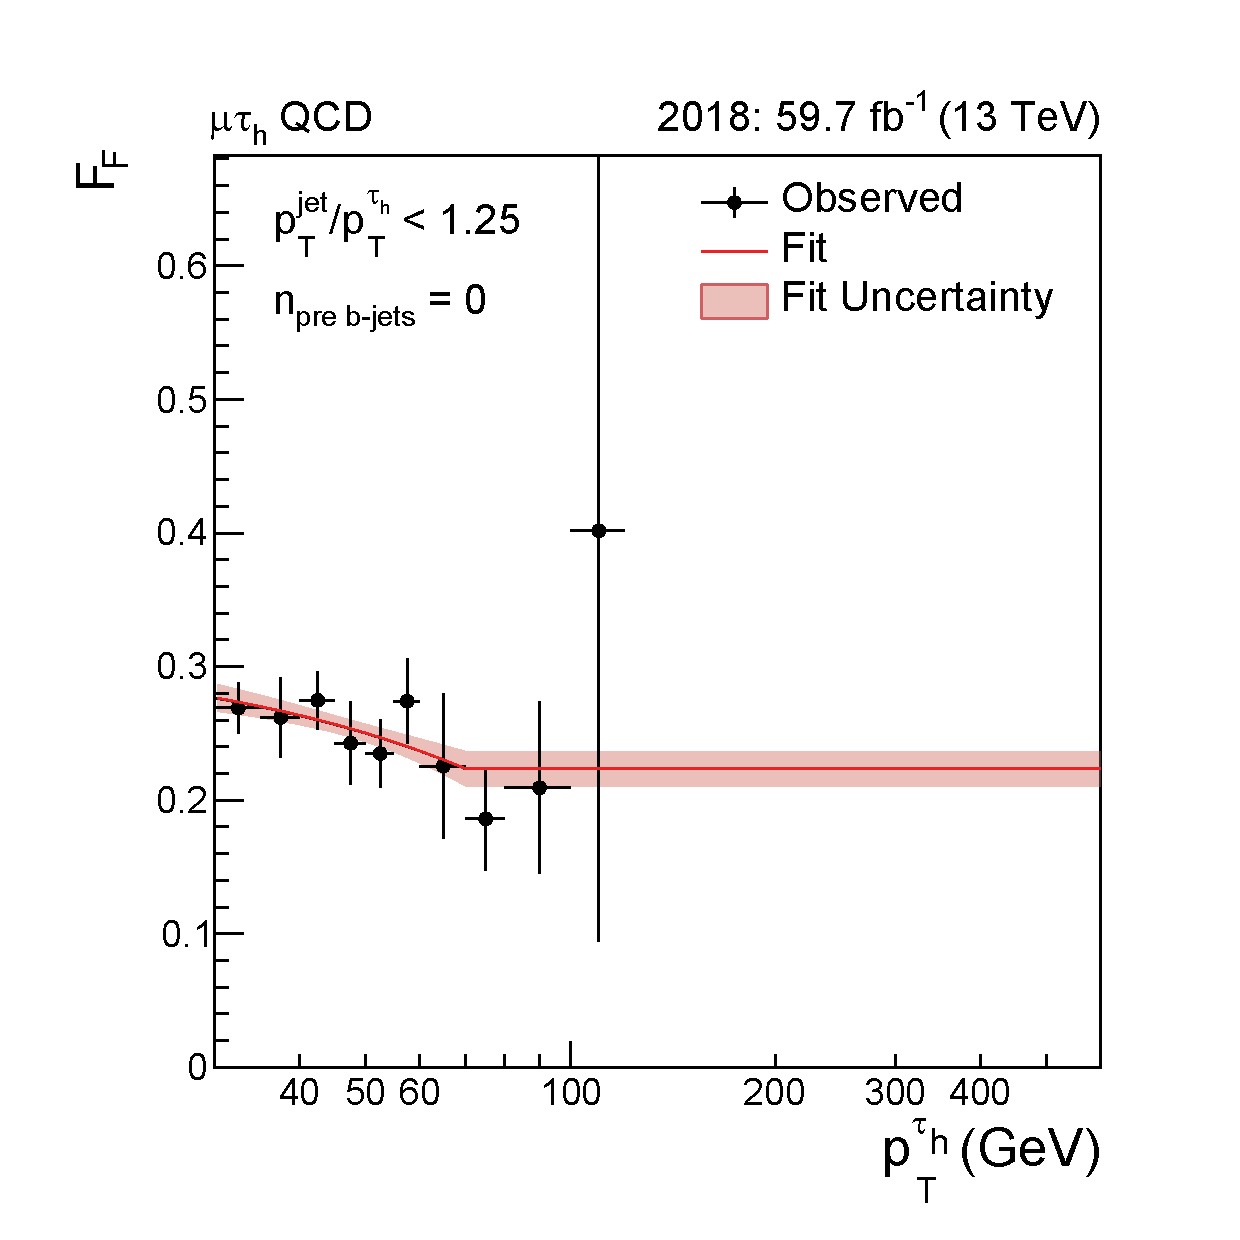
\includegraphics[width=0.33\textwidth]{Figures/ff_fit_jet_pt_low_0jet_pt_2_ff_qcd_mt_2018-EK.pdf}}
    \subfloat[]{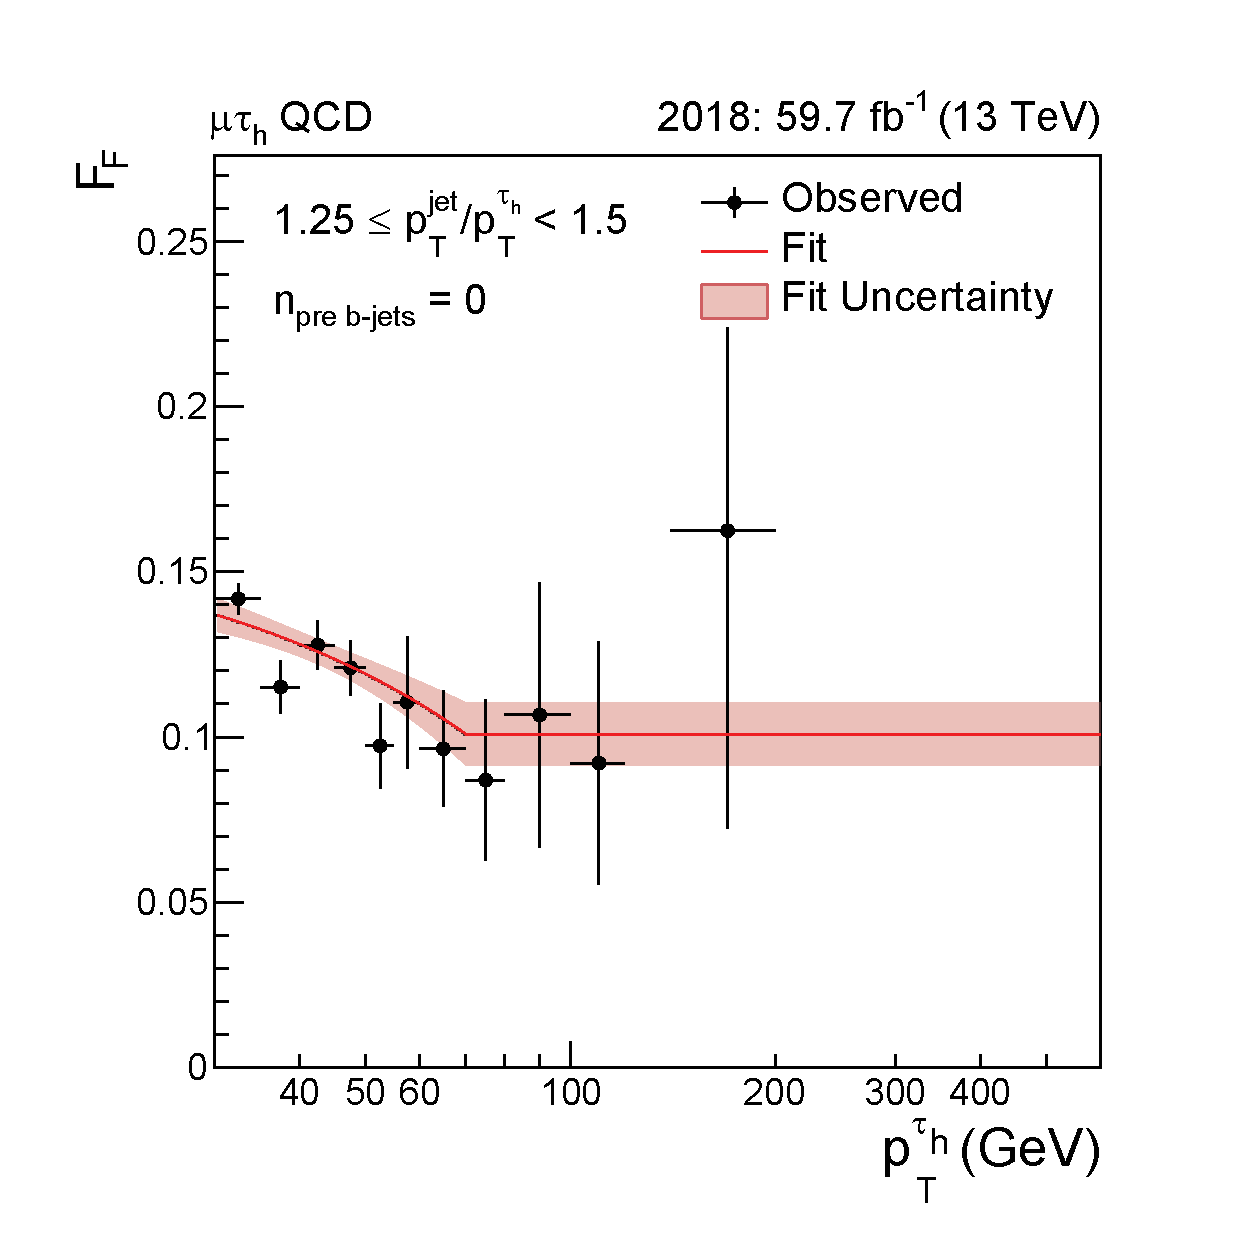
\includegraphics[width=0.33\textwidth]{Figures/ff_fit_jet_pt_med_0jet_pt_2_ff_qcd_mt_2018-EK.pdf}} 
    \subfloat[]{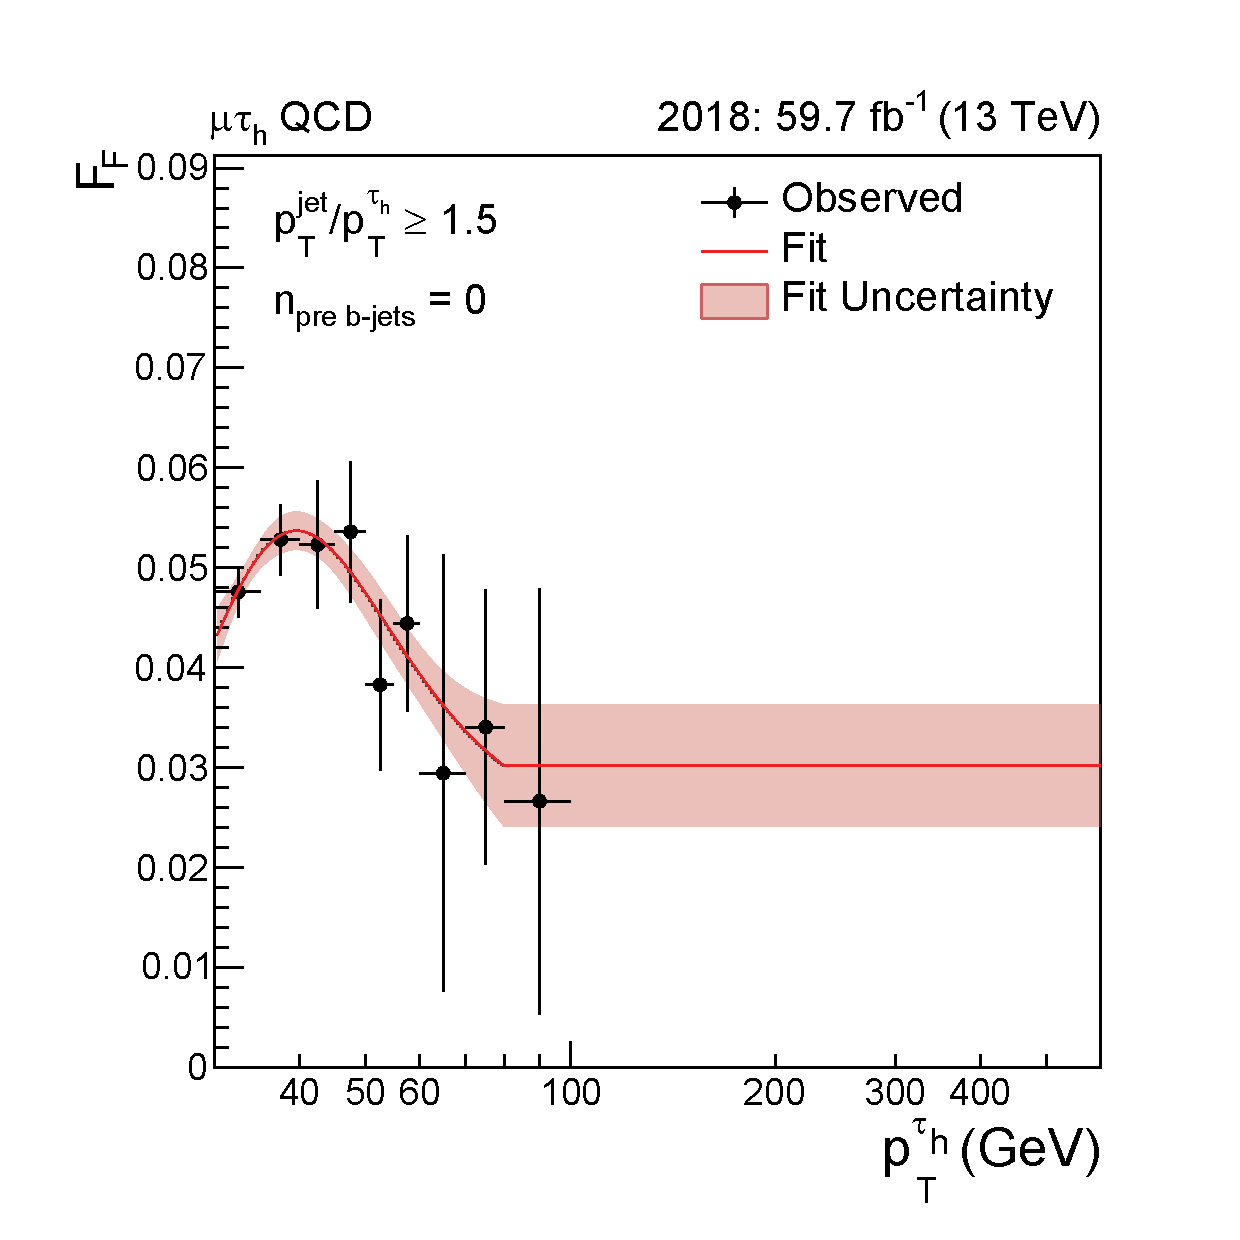
\includegraphics[width=0.33\textwidth]{Figures/ff_fit_jet_pt_high_0jet_pt_2_ff_qcd_mt_2018-EK.pdf}} \\
    \subfloat[]{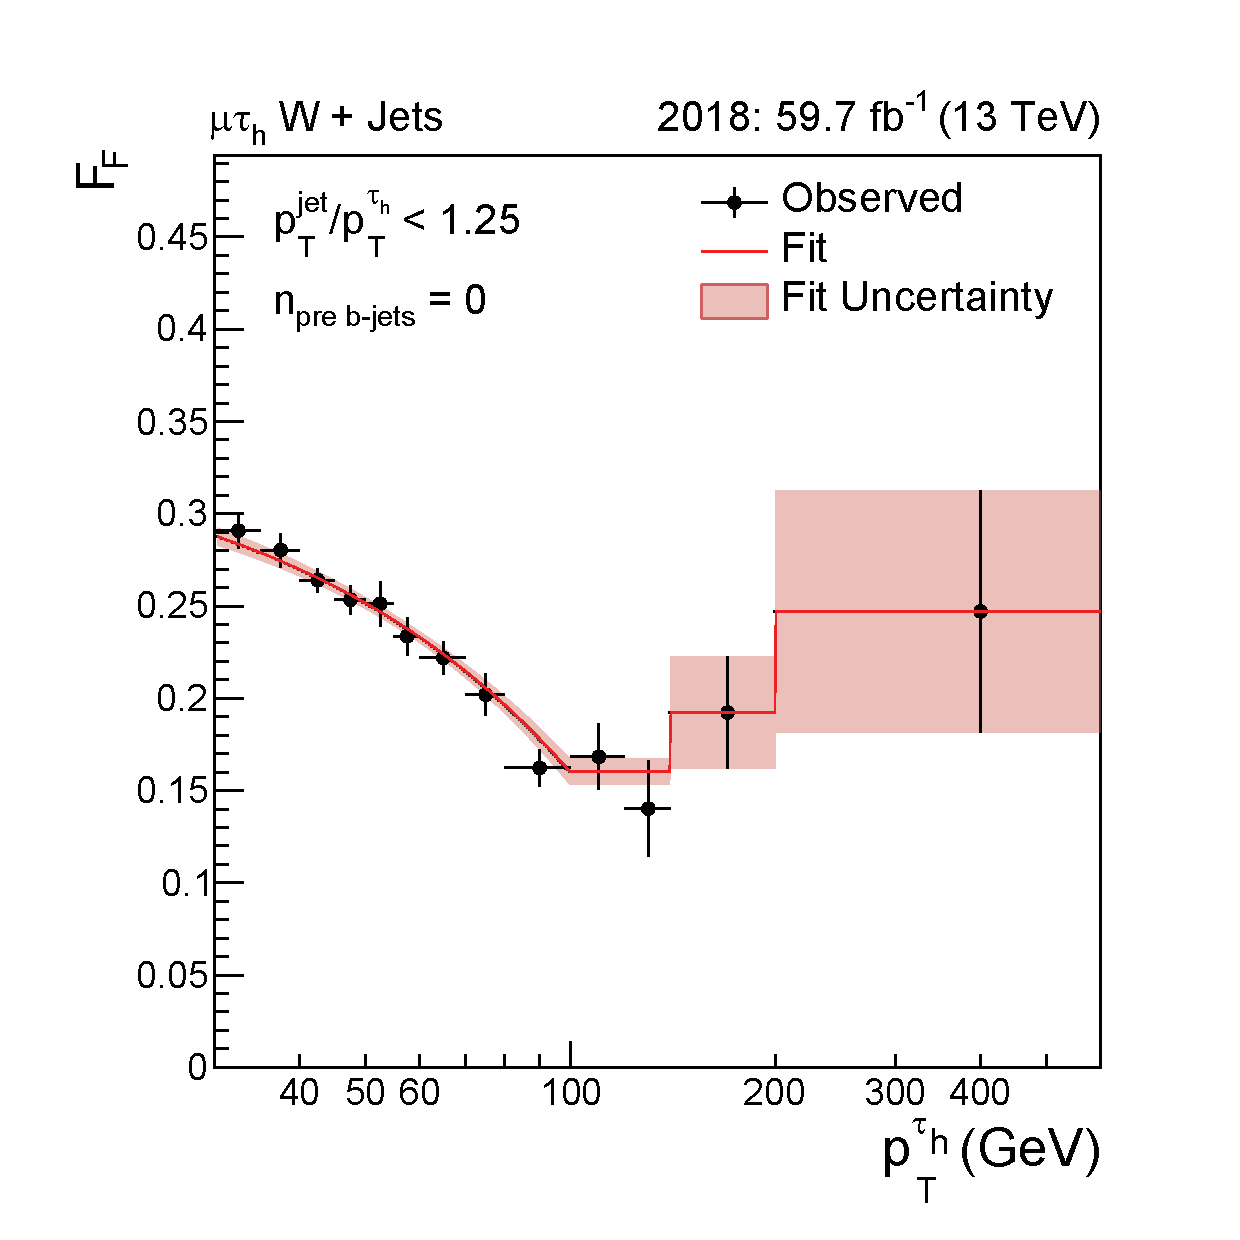
\includegraphics[width=0.33\textwidth]{Figures/ff_fit_jet_pt_low_0jet_pt_2_ff_wjets_mt_2018-EK.pdf}}
    \subfloat[]{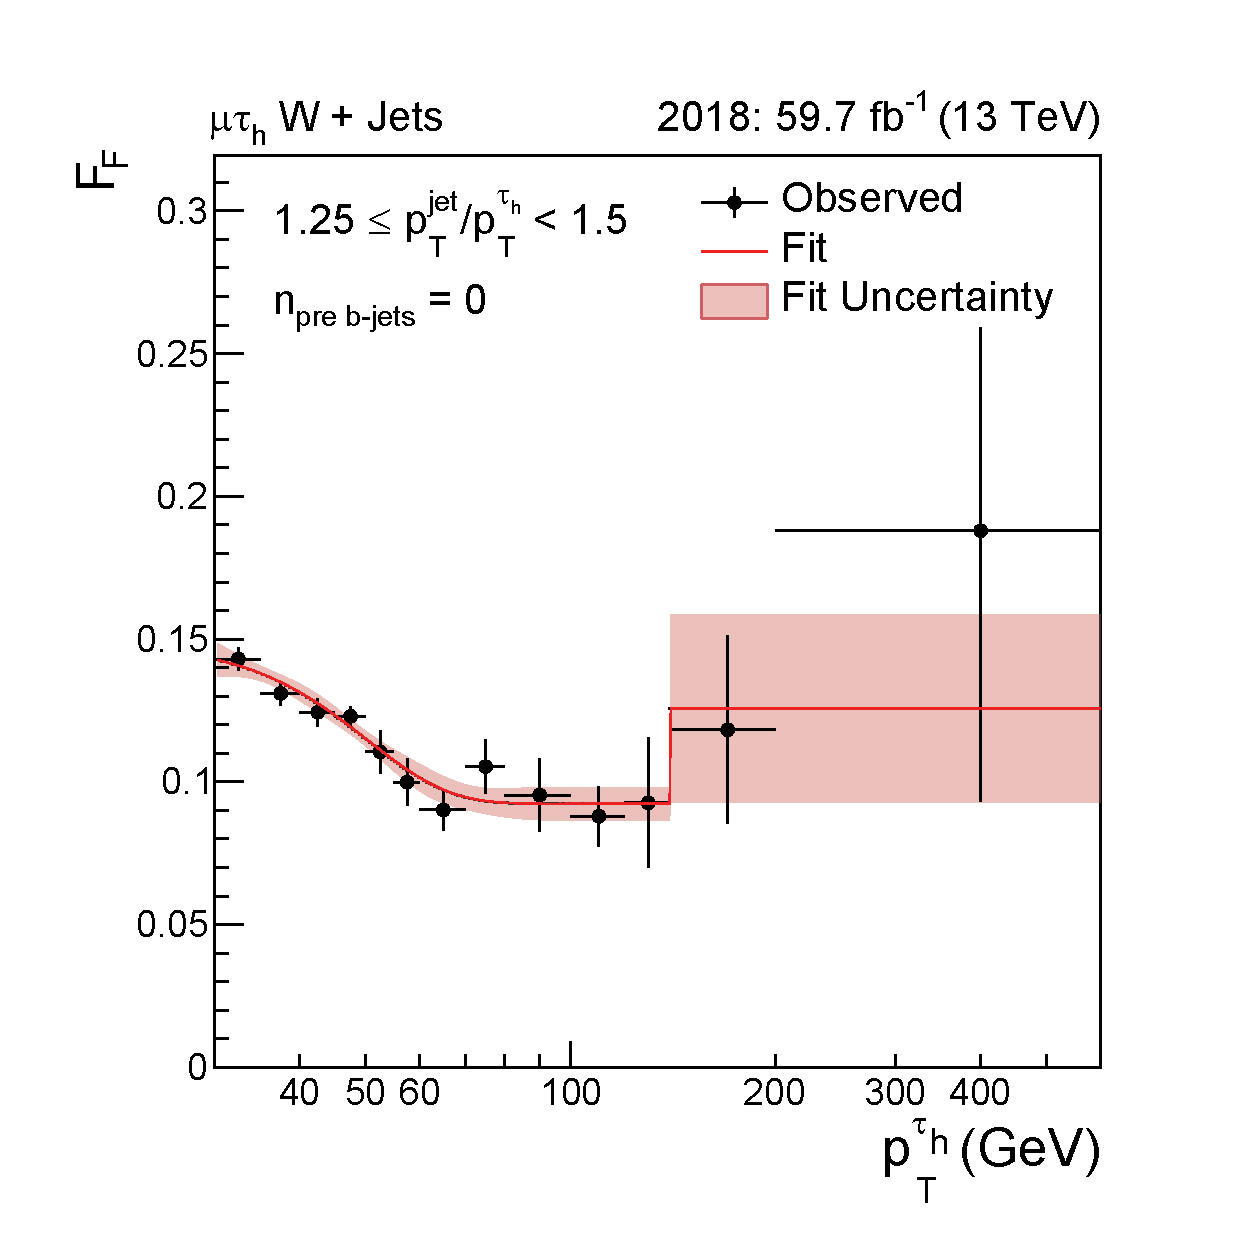
\includegraphics[width=0.33\textwidth]{Figures/ff_fit_jet_pt_med_0jet_pt_2_ff_wjets_mt_2018-EK.pdf}} 
    \subfloat[]{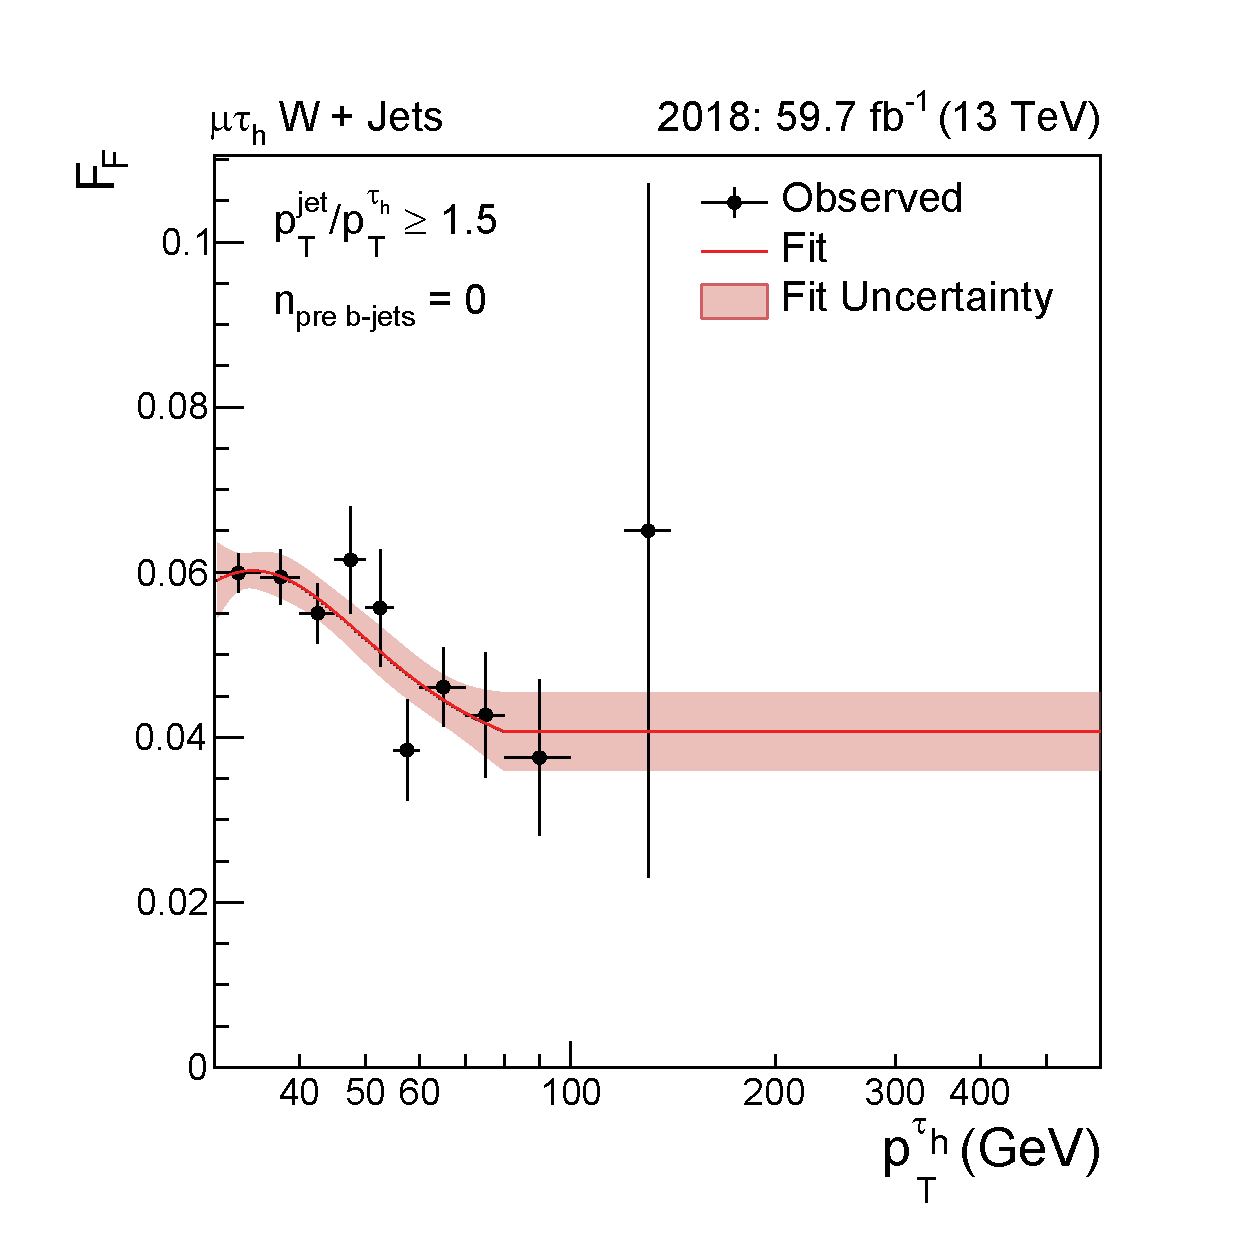
\includegraphics[width=0.33\textwidth]{Figures/ff_fit_jet_pt_high_0jet_pt_2_ff_wjets_mt_2018-EK.pdf}} \\
\caption[Plots of the fake factor fits in the $\mu\tauh$ channel.]{$\FF$ fits in $\mu\tauh$ channel for the QCD and W + Jets $N_{\text{pre b jets}}=0$ category with 2018 data. The three jet $\pT$ to $\tau_h$ $\pT$ categories are shown for each process.}
\label{fig:mt_ff_fit}
\end{figure}

\subsection{Corrections}

In the $\tauhtauh$ channel, the measured $\FF$ are then corrected to account for non-closures in other variables in the \texttt{Determination Region}. 
The only significant non-closures are observed for $\MET$ related variables and are largest for events with $N_{\text{pre b jets}}=0$. 
Closure corrections are performed for the variable $\Delta R$ between the $\tauh$ candidates in bins of $N_{\text{b jets}}$.
In the $\mutauh$ and $\etauh$ channels, the measured QCD and W + jets $\FF$ are corrected for non-closures observed in the $\MET$ variables and $\pT^{e/\mu}$ distributions.
A study was performed to determine the nature of these non-closures and it was found that the cause was due to fake \ac{MET} arising from mismeasurement of the energies of particles in a jet. 
If a jet's energy is mismeasured, this is also propagated to the reconstruction of the \ac{MET} and the $\tauh$ candidate and there will be a specific alignment between these objects if no neutrinos are present in the event.
A mismeasurement of the jet energy can alter the $\tauh$ isolation and so it can also affect the identification scores, and this shift can be accounted for with some measure of the fake \ac{MET}.
A diagram of this effect is shown in Figure~\ref{fig:fakemet}. \\

\begin{figure}[!hbtp]
\centering
   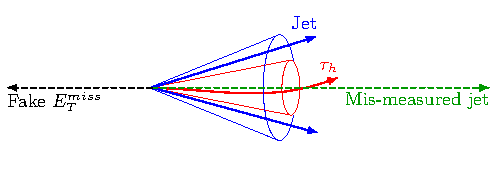
\includegraphics[width=\textwidth]{Figures/fakemet_plot.pdf}
\caption[Diagram of the fake MET alignment with the $\tauh$ candidate.]{Diagram showing how fake MET arises from mis-modelling jet energies and how it can align with the $\tauh$ candidate identified.}
\label{fig:fakemet}
\end{figure}

To correct for this effect, the QCD $\FF$ are corrected as a function of $C_{\text{QCD}}$, where $C_{\text{QCD}}$ is defined as,
\begin{equation}
C_{\text{QCD}} = \frac{\MET \cos\Delta\phi(\pTvec^{\text{\hspace{2pt}miss}},\pTvec^{\hspace{2pt}\tauh})}{\pT^{\tauh}}.
\label{eqn:c_qcd}
\end{equation}
where $\Delta\phi(\pTvec^{\hspace{2pt}\text{miss}},\pTvec^{\hspace{2pt}\tauh})$ is the separation in the azimuthal angle between the missing transverse momentum vector $\pTvec^{\hspace{2pt}\text{miss}}$ and $\pTvec^{\hspace{2pt}\tauh}$.
The numerator quantifies the missing transverse momentum in the direction of the $\tau_h$ candidate. 
Once divided by the $\tauh$ $\pT$, $C_{\text{QCD}}$ is a measure of the fraction of missing to visible $\tau_h$ transverse momentum aligned with the $\tau_h$.
For W + jets and $\ttbar$ the situation is slightly different due to the presence of genuine missing energy from neutrinos.
In this case, the correction variable is modified to approximately subtract the genuine \ac{MET} from the total.
This approximation assumes the neutrino is back-to-back and balanced with the light lepton (which is exactly true for W bosons produced at rest in the transverse direction). 
The equation then becomes,
\begin{equation}
C_{\text{W}} = \frac{(\MET+\pT^{e/\mu}) \cos\Delta\phi(\pTvec^{\text{\hspace{2pt}miss}}+\pTvec^{\hspace{2pt}e/\mu},\pTvec^{\hspace{2pt}\tauh})}{\pT^{\tauh}}.
\label{eqn:c_w}
\end{equation}
When either correction variable is non-zero, a larger quantity of fake \ac{MET} is expected in the event. 
In these regions, a large correction is needed due to the mismeasured jet energy spectrum shifting the $\tau_h$ candidate isolation and so shifting the $\tau$ identification scores. 
Examples of these closure corrections are shown in Figure~\ref{fig:ff_dr}\\

After the \texttt{Determination Region} is modelled well for all variables of interest, extrapolation corrections from the $\FF$ derived in B applied to region D are calculated.
In the $\tauhtauh$ the correction is parametrised by the $p_{T}$ of the leading $\tau_h$ candidate, in the $\etauh$ and $\mutauh$ channels it is parametrised by the $\pT$ of the light lepton.
Where statistics allow, these corrections are calculated in the high-mass optimisation procedure categories.
Examples of the extrapolation corrections are shown in Figure~\ref{fig:ff_dr_to_ar}.

\begin{figure}[!hbtp]
\centering
    \subfloat[]{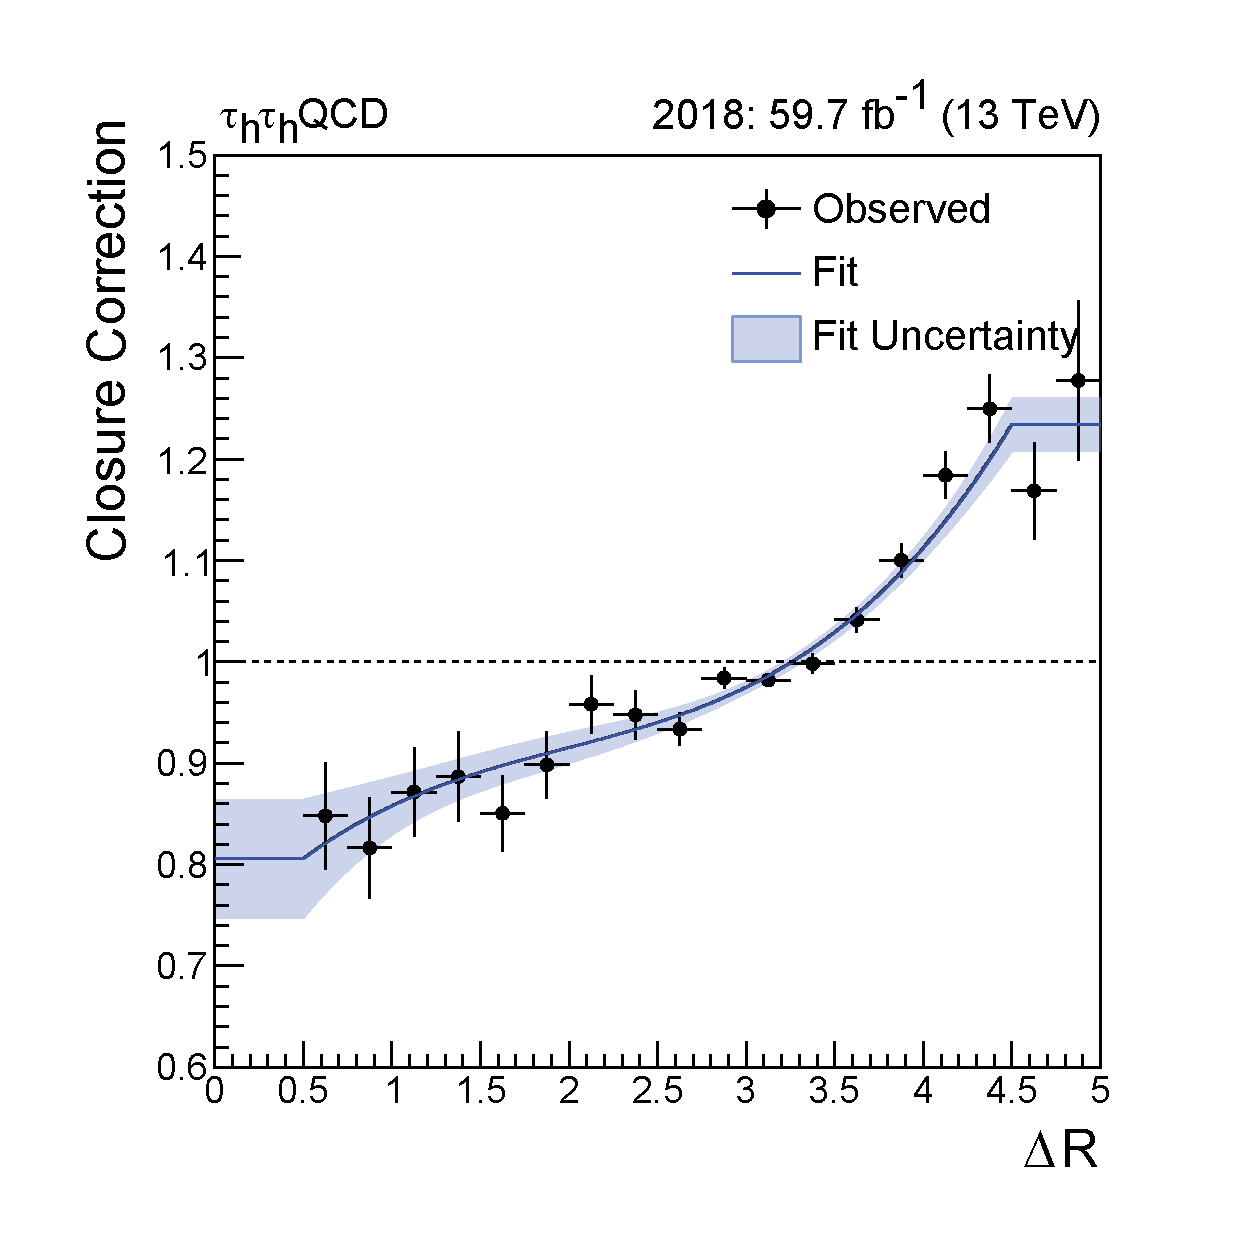
\includegraphics[width=0.33\textwidth]{Figures/ff_closure_ss_closure_nbjet0_qcd_tt_2018_v2-EK.pdf}} 
    \subfloat[]{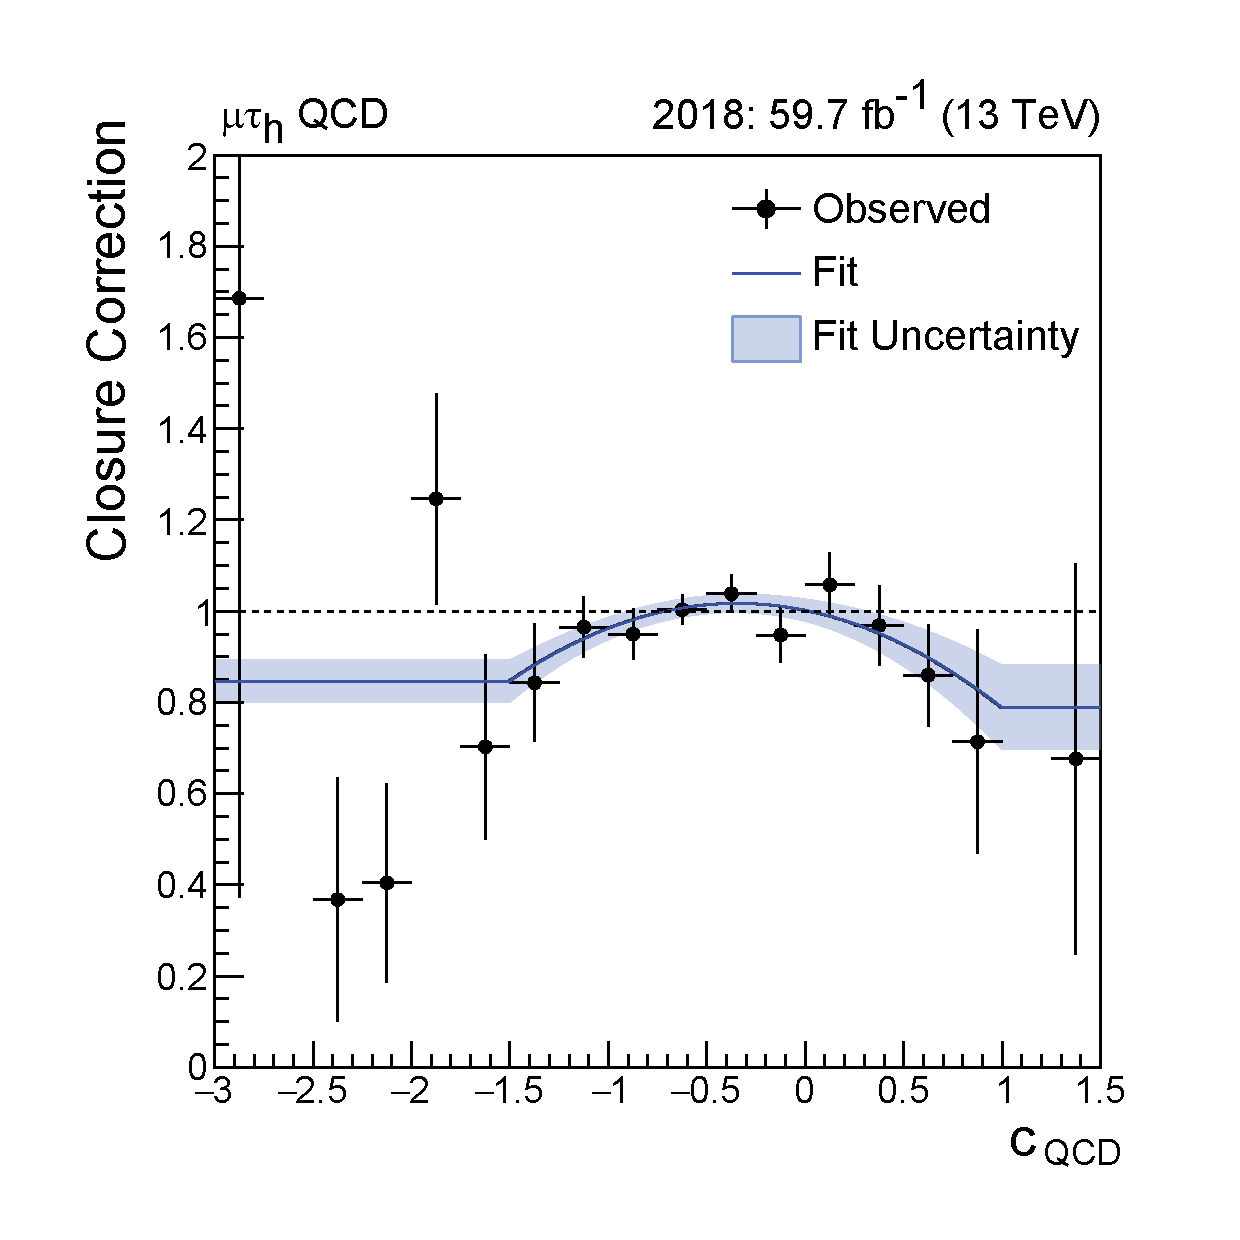
\includegraphics[width=0.33\textwidth]{Figures/ff_closure_met_0jet_closure_qcd_mt_2018-EK.pdf}}
    \subfloat[]{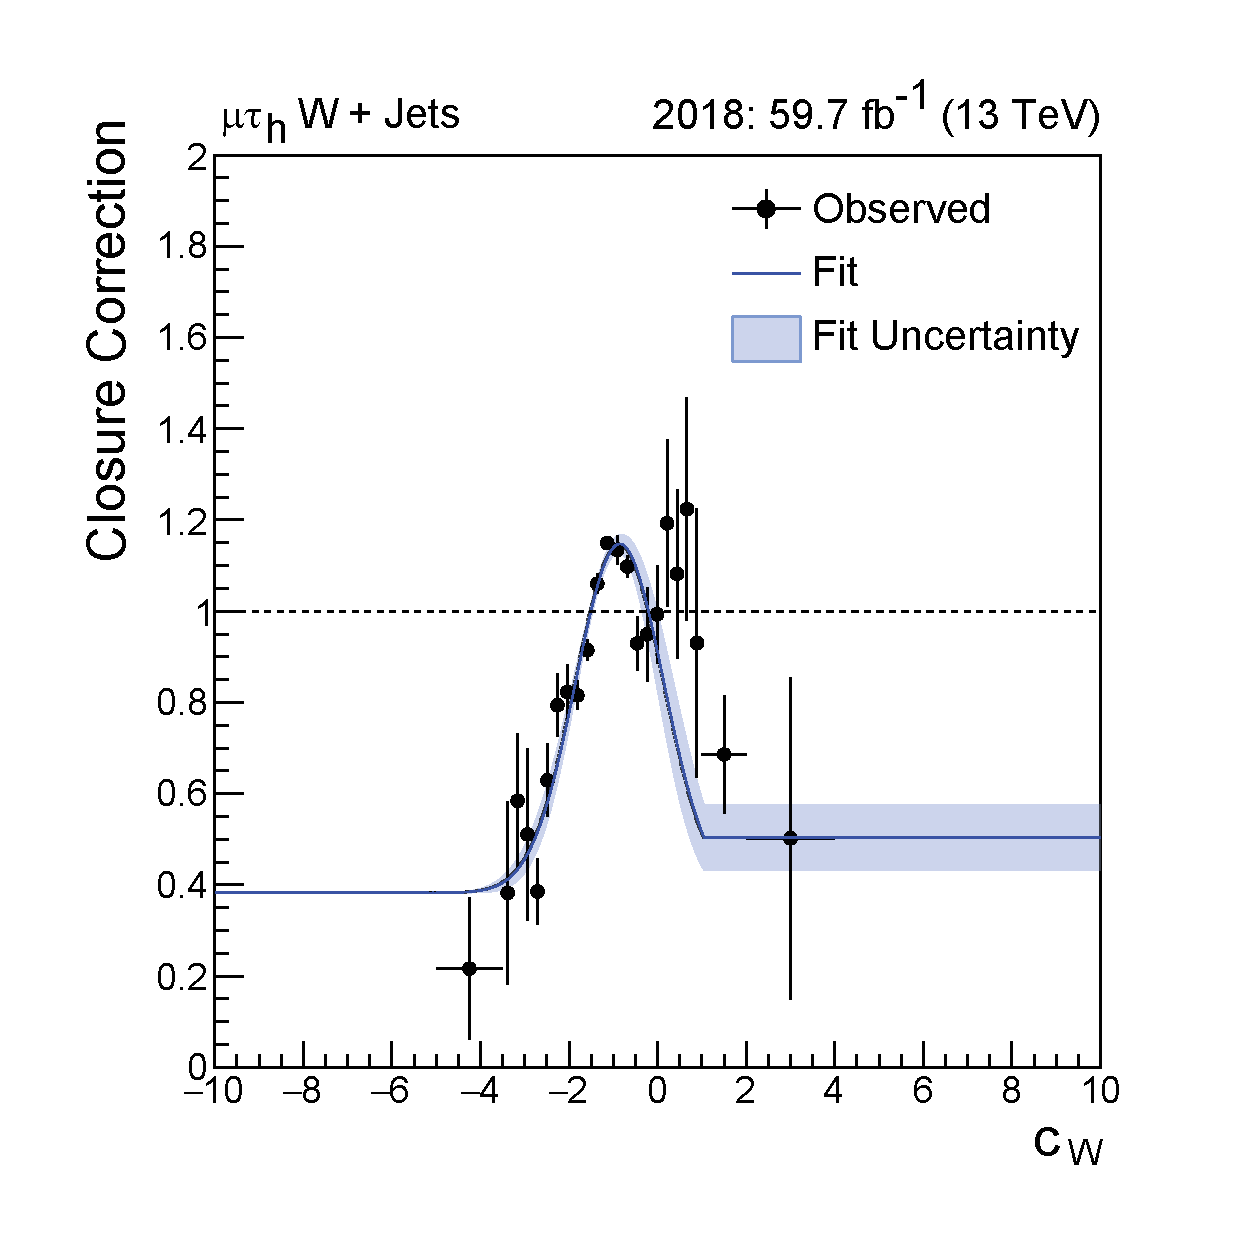
\includegraphics[width=0.33\textwidth]{Figures/ff_closure_met_0jet_closure_wjets_mt_2018-EK.pdf}}
\caption[Plots of fake factor \texttt{Determination Region} closure correction fits.]{\texttt{Determination Region} closure correction fits with 2018 data. (a) is the correction parametrised by $\Delta R$ in events with $N_{\text{b jets}}=0$ in the $\tauhtauh$ channel. (b) and (c) show the correction for the $\mutauh$ channel parametrised by the specific correction variables defined in Equations~\ref{eqn:c_qcd} and \ref{eqn:c_w} for QCD and W + jets processes respectively.}
\label{fig:ff_dr}
\end{figure}

\begin{figure}[!hbtp]
\centering
    \subfloat[]{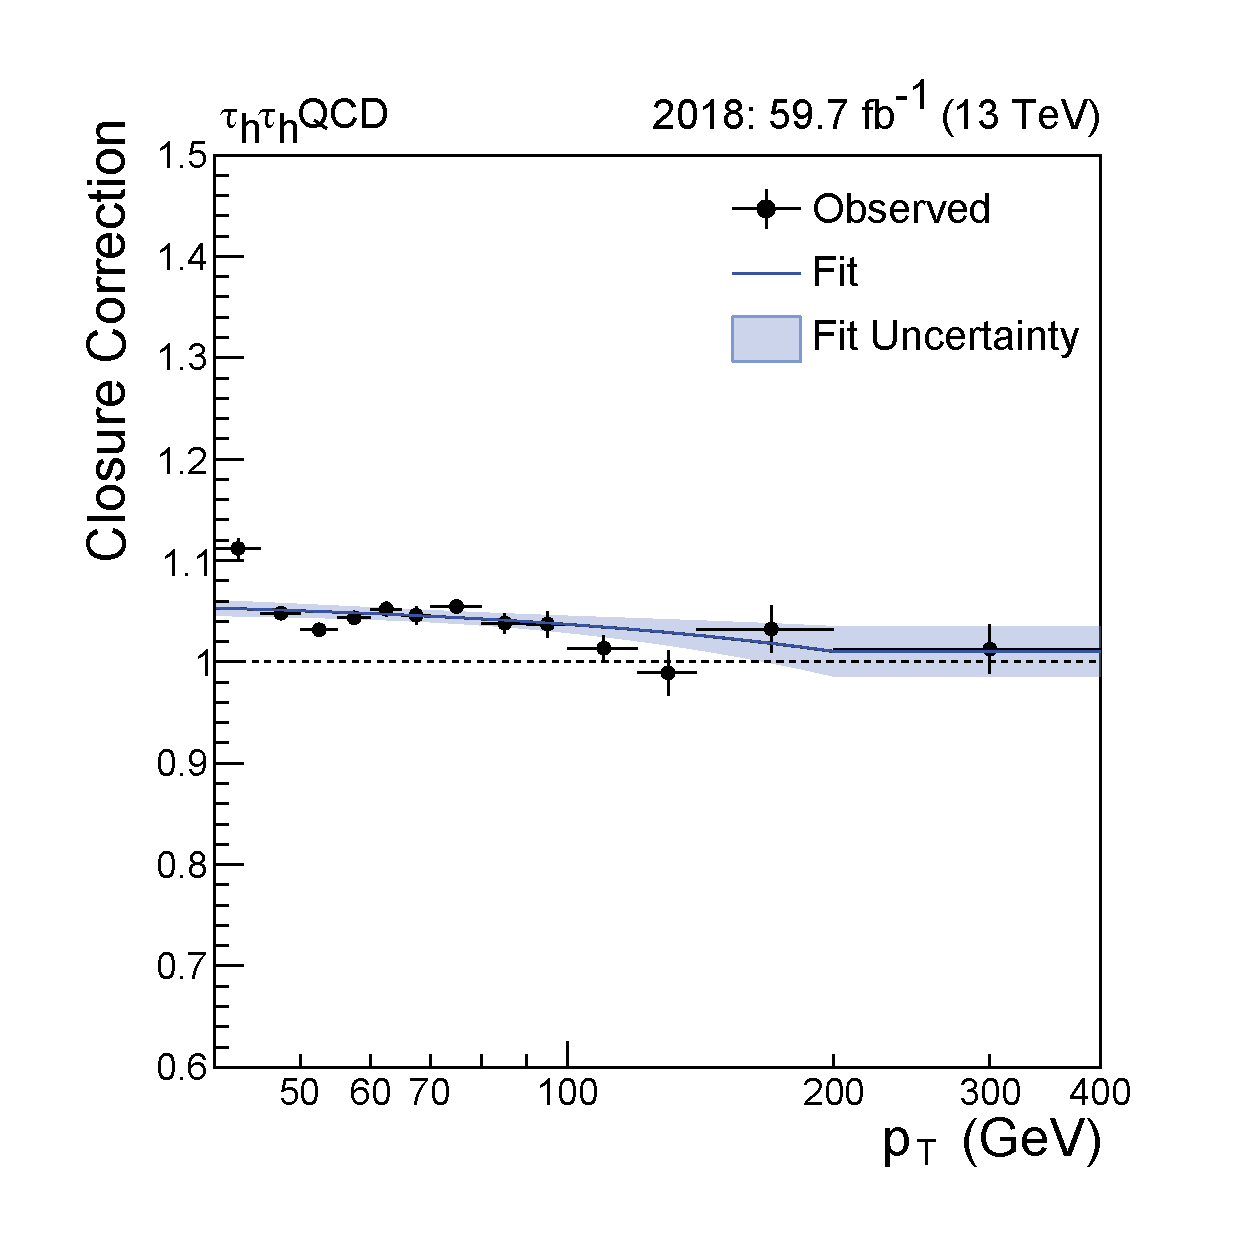
\includegraphics[width=0.33\textwidth]{Figures/ff_closure_os_closure_nbjet0_alt_qcd_tt_2018_v2-EK.pdf}} 
    \subfloat[]{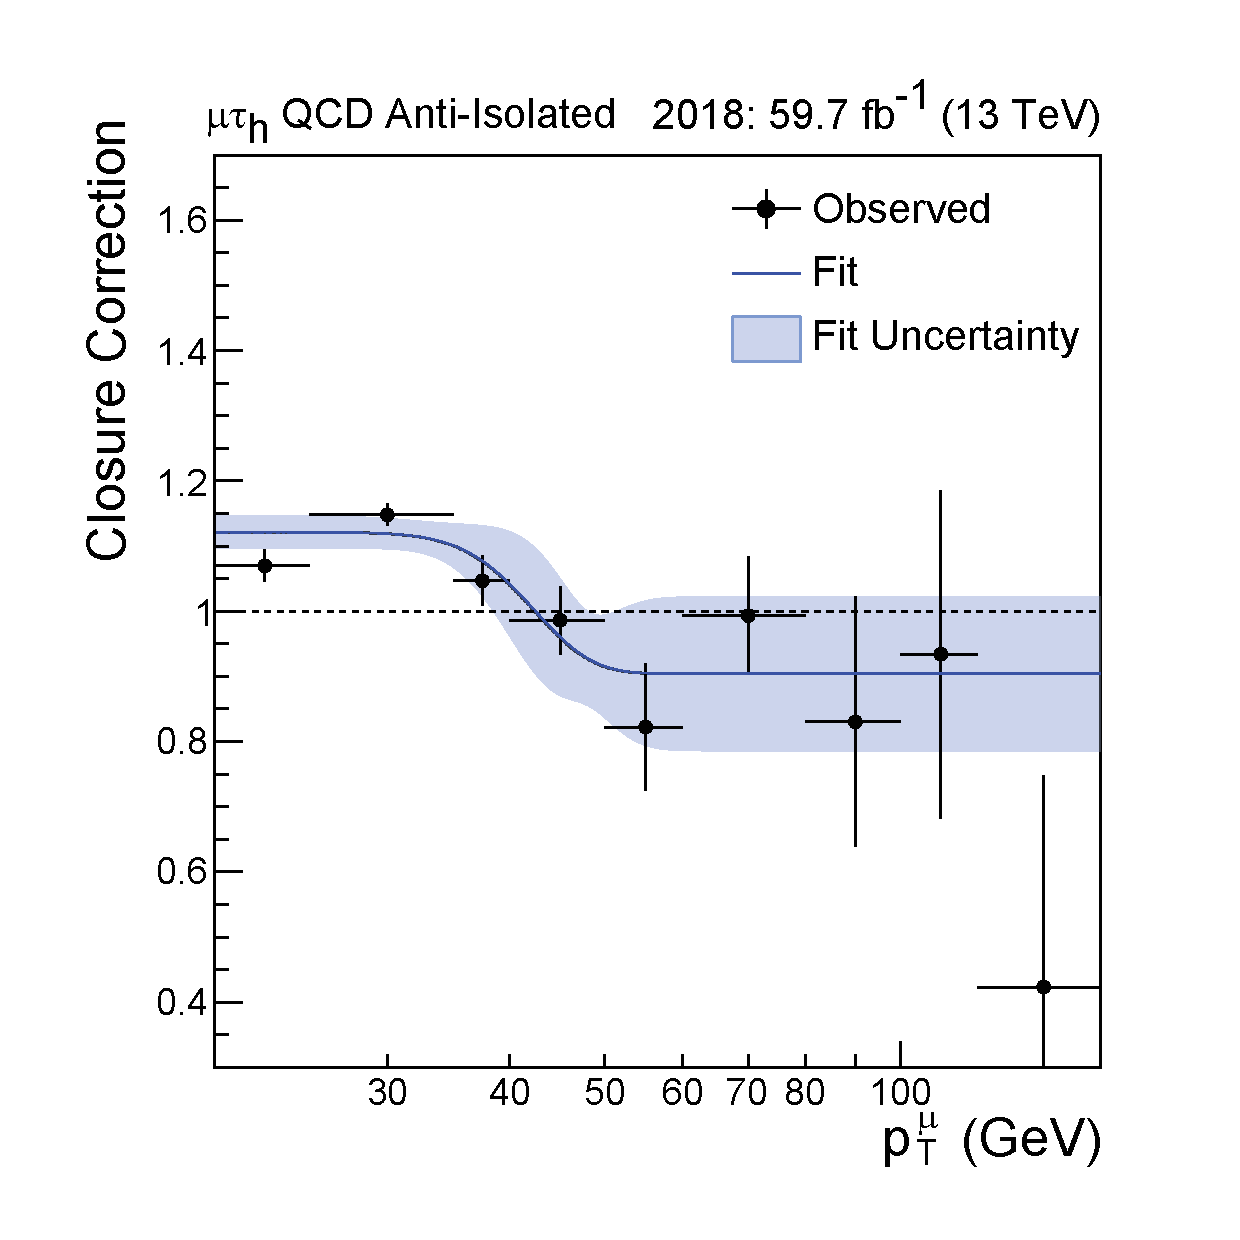
\includegraphics[width=0.33\textwidth]{Figures/ff_closure_pt_1_nbjets0_dr_to_ar_aiso_closure_qcd_mt_2018-EK.pdf}}
    \subfloat[]{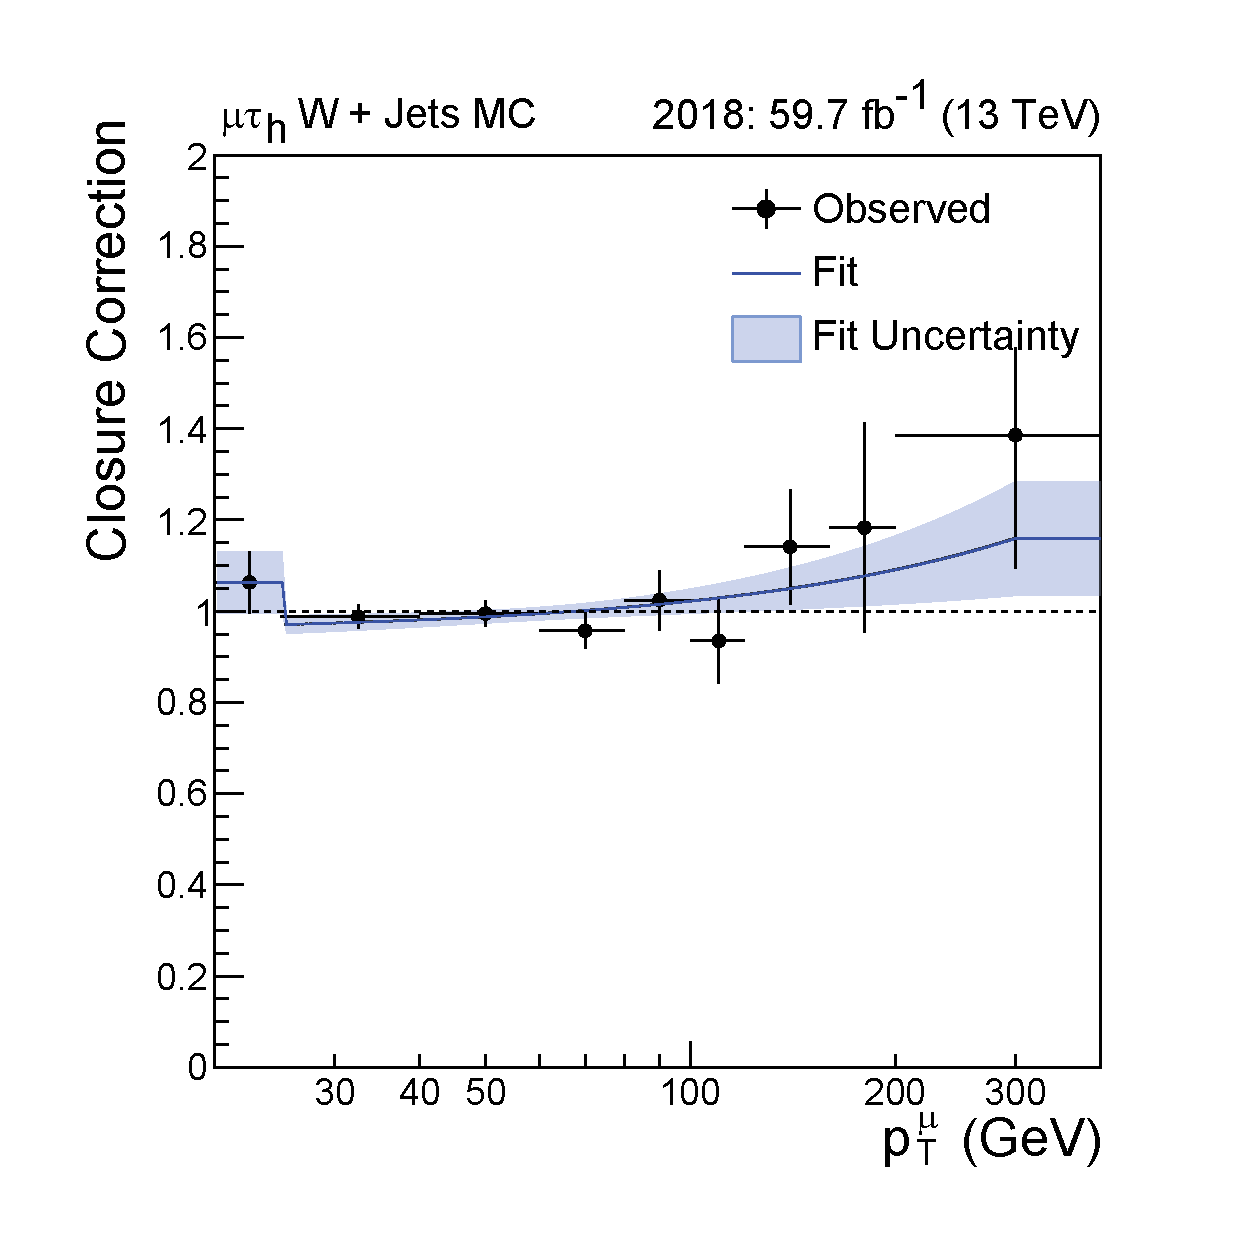
\includegraphics[width=0.33\textwidth]{Figures/ff_closure_pt_1_nbjets0_tightmt_dr_to_ar_closure_wjets_mc_mt_2018-EK.pdf}}
\caption[Plots of fake factor \texttt{Determination Region} to \texttt{Application Region} closure correction fits.]{\texttt{Determination Region} to \texttt{Application Region} closure correction fits with 2018 data. (a) is the correction moving from same sign to opposite sign $\tau$ leptons the parametrised by leading $\tauh$ $\pT$ in events with $N_{\text{b jets}}=0$ in the $\tauhtauh$ channel. (b) and (c) show the correction for the $\mutauh$ channel moving from same sign to opposite sign $\tau$ leptons and high $m_{T}$ to low $m_{T}$ both parametrised by the muon $\pT$ for QCD and W + jets processes respectively.}
\label{fig:ff_dr_to_ar}
\end{figure}

\subsection{Applying fake factors}
\label{sec:ff_applying}

In the $\etauh$ and $\mutauh$ channels, the $\FFi$ measured for the different processes, $i$, are combined into an overall factor $\FF$ using,
\begin{equation}
\FF = \sum_{i}f_{i}\cdot \FFi,
\end{equation}
where the factor $f_{i}$ is defined as,
\begin{equation}
f_{i} = \frac{N_{\text{AR}}^{i}}{\sum\limits_{j}N_{\text{AR}}^{j}},
\end{equation}
which is the fraction of events with a \jtth originating from process $i$ over the total number of \jtth events for all processes in the \texttt{Application Region}.
These fractions of events are estimated with \ac{MC}, with a \ac{QCD} model extrapolated from same sign $\tau$ pairs, and examples are shown in Figure~\ref{fig:mt_ff_frac}.
It is observed that W + jets is the dominating process in this region, however, there are effects from \ac{QCD} at low $\mT$ and from $\ttbar$ in the b-tagged categories. 
These fractions are then multiplied by the relevant corrected $\FF$ and applied to the fail $\tauh$ identification region in C, where this region is purified by subtracting any non \jtth events with \ac{MC}. \\

\begin{figure}[!hbtp]
\centering
    \subfloat[]{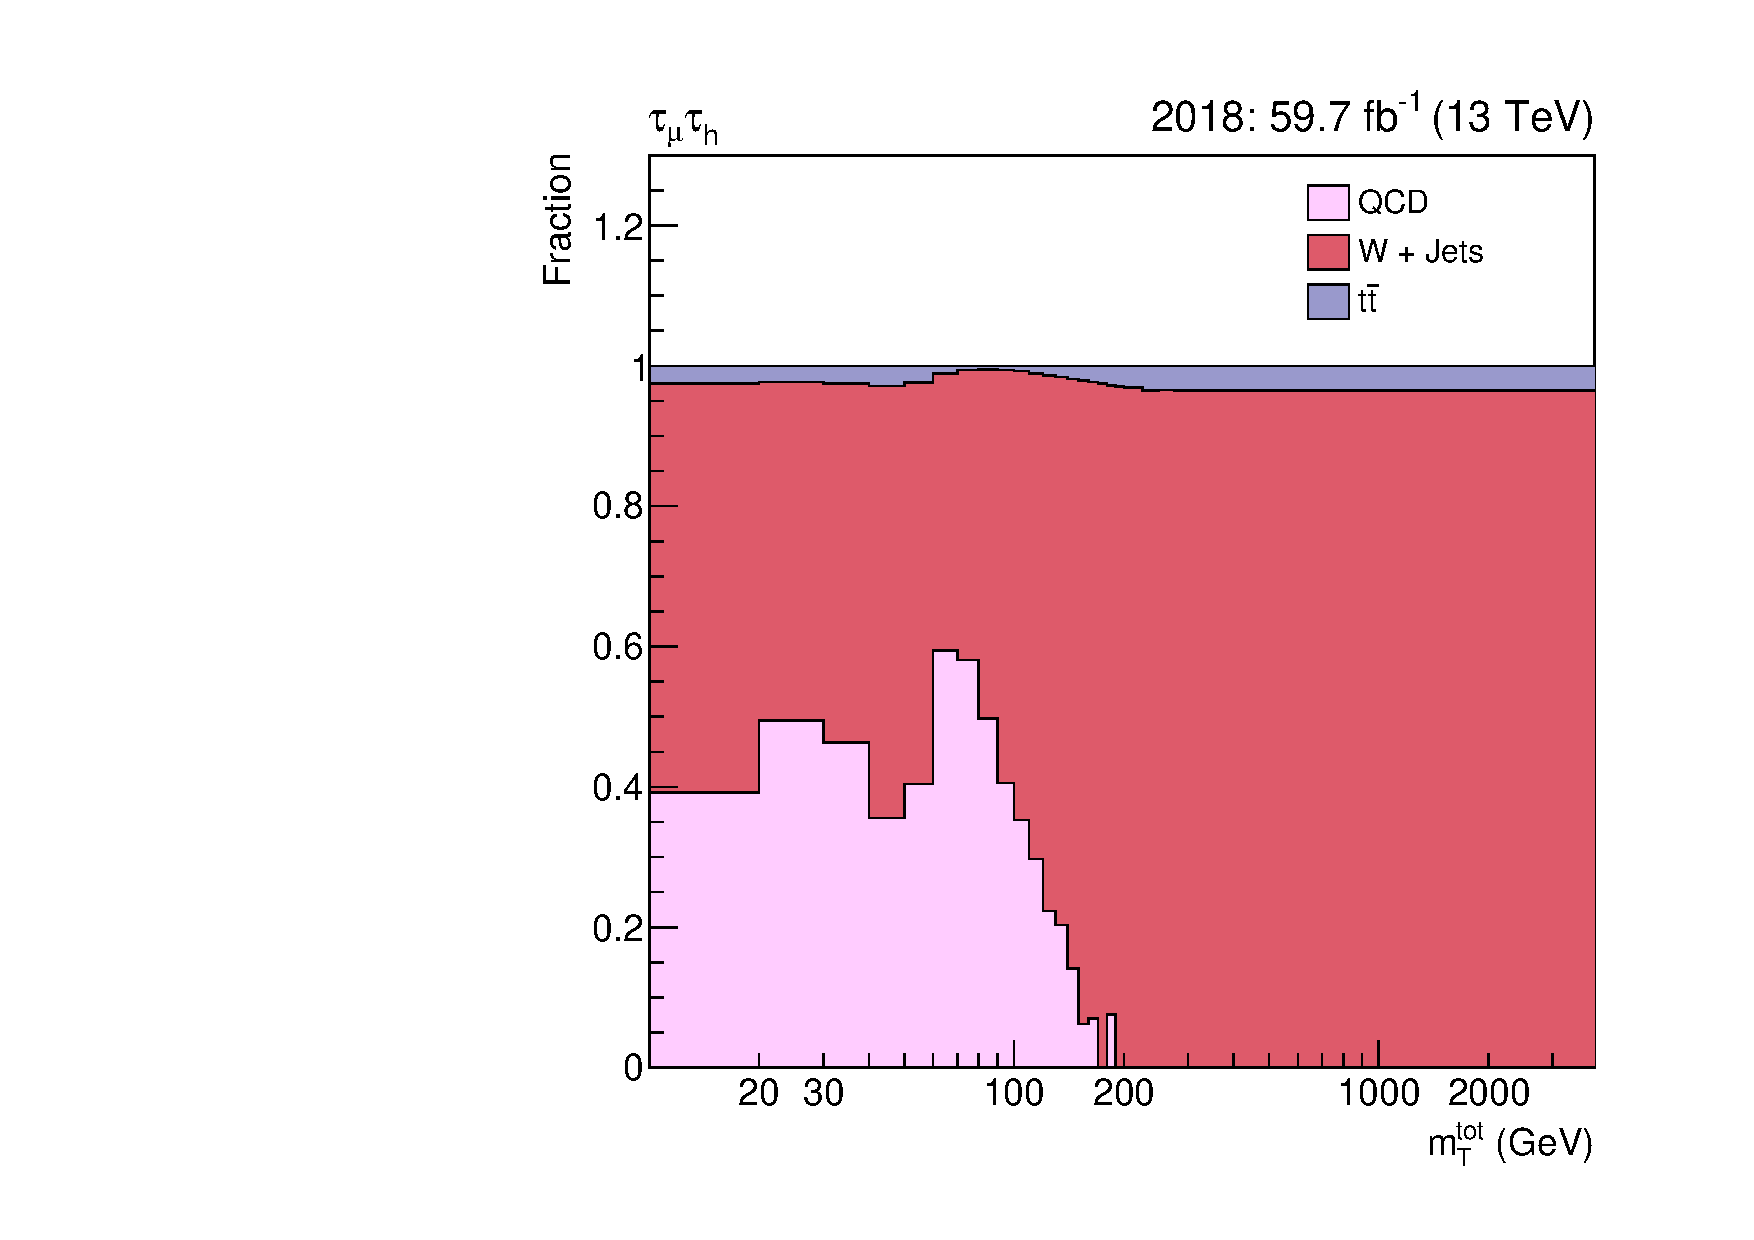
\includegraphics[width=0.45\textwidth]{Figures/ff_fraction_tightmt_nbjets0_mt_2018_os_rebinning.pdf}}
    \subfloat[]{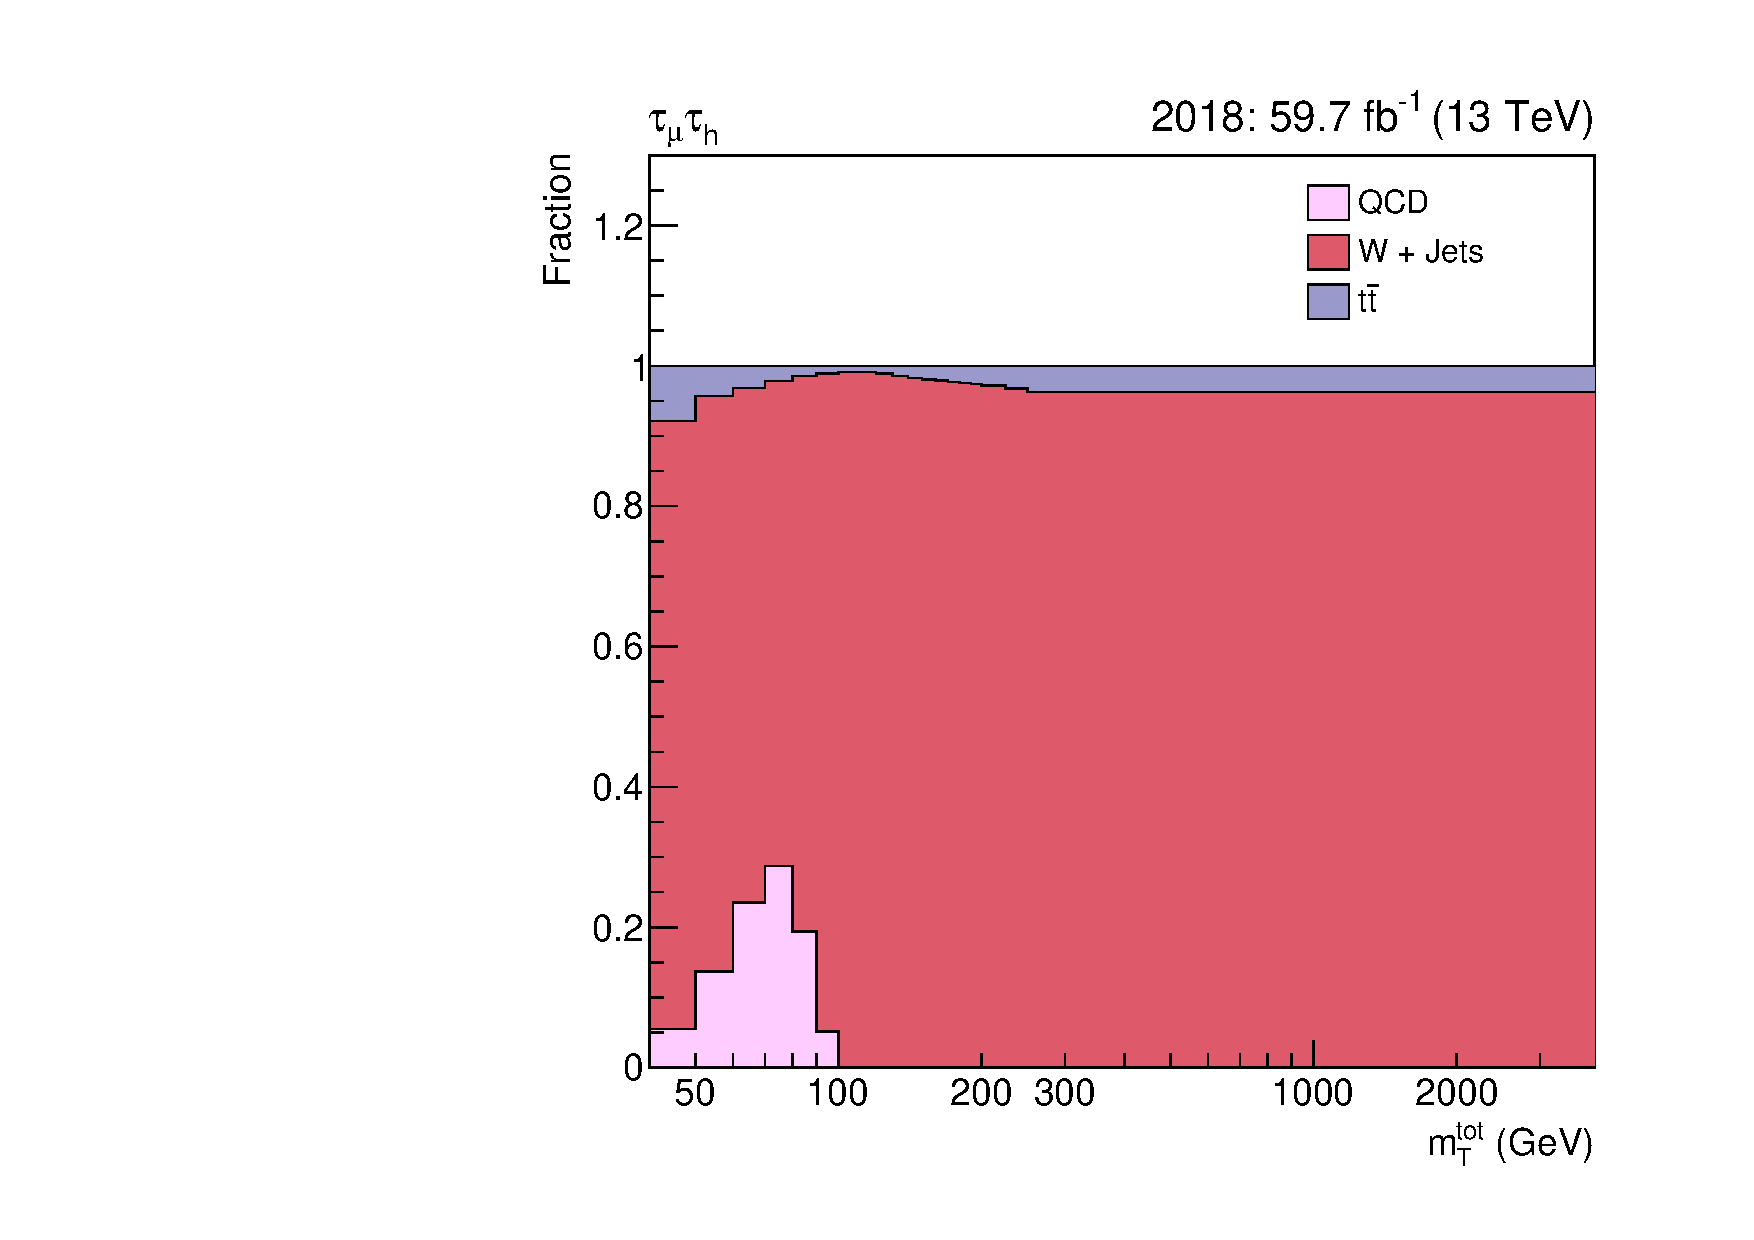
\includegraphics[width=0.45\textwidth]{Figures/ff_fraction_loosemt_nbjets0_mt_2018_os_rebinning.pdf}} \\
    \subfloat[]{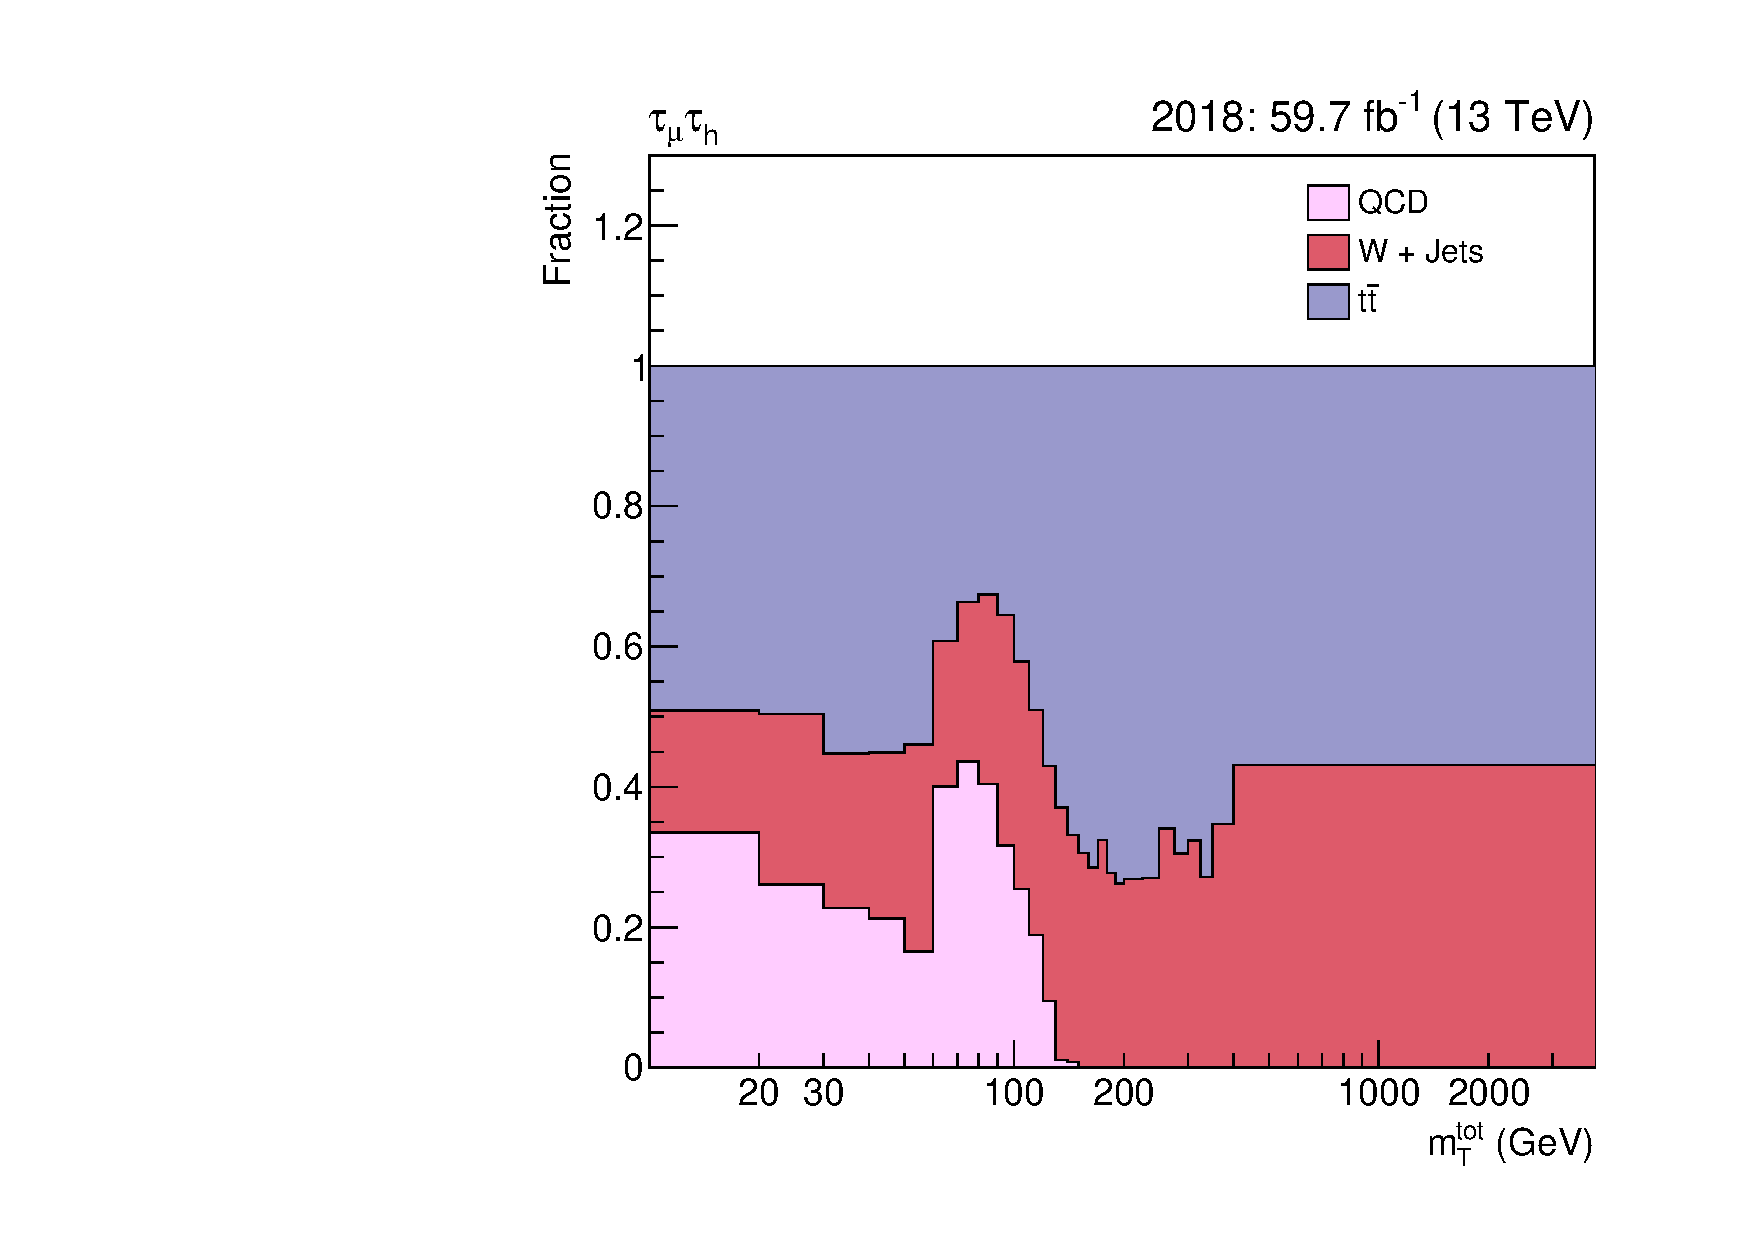
\includegraphics[width=0.45\textwidth]{Figures/ff_fraction_tightmt_nbjets1_mt_2018_os_rebinning.pdf}}
    \subfloat[]{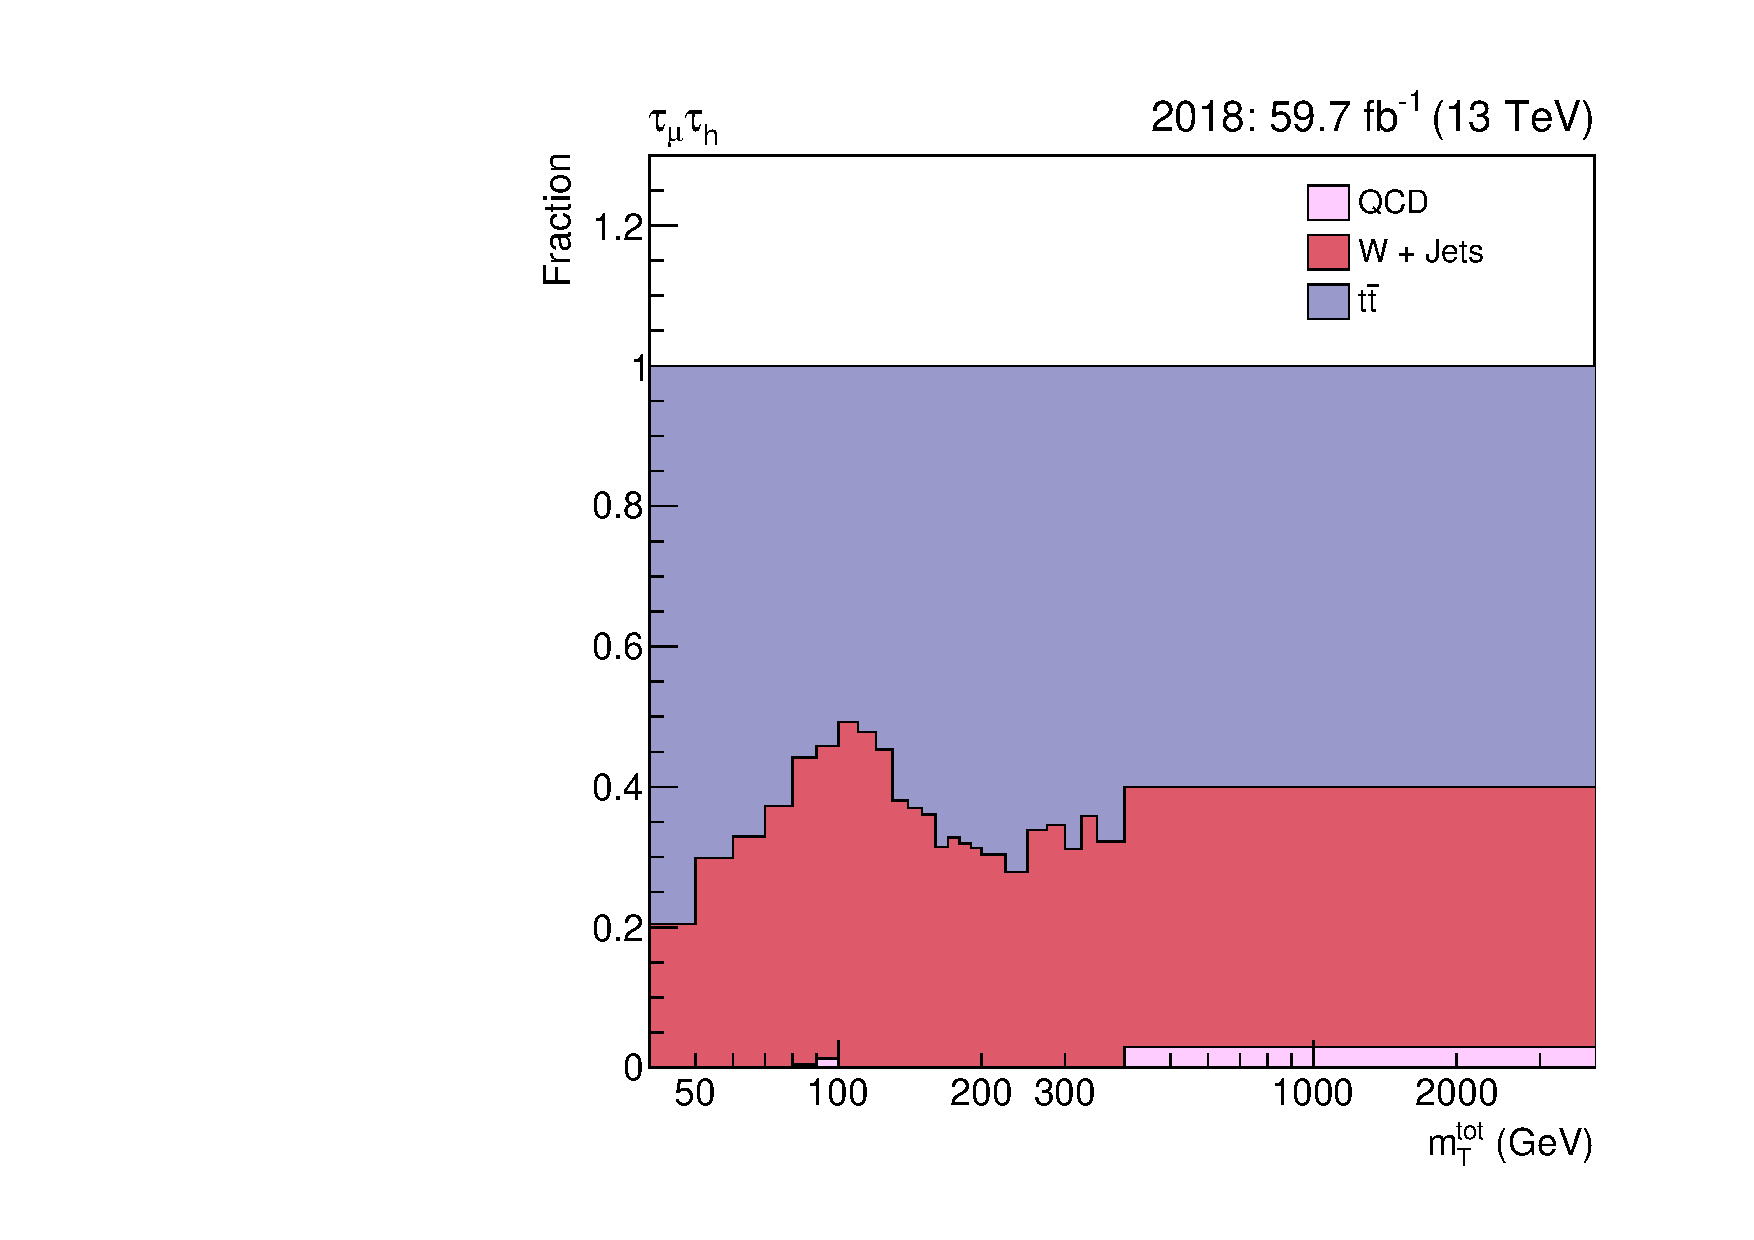
\includegraphics[width=0.45\textwidth]{Figures/ff_fraction_loosemt_nbjets1_mt_2018_os_rebinning.pdf}} \\
\caption[Plots of the expected fake factor \texttt{Application Region} fractions of the processes in the $\mutauh$ channel.]{The expected \texttt{Application Region} fractions of the processes in the $\mutauh$ channel. (a) and (b) show the no b tag \texttt{Tight-$m_{T}$} and \texttt{Loose-$m_{T}$} categories and (c) and (d) show the b tag \texttt{Tight-$m_{T}$} and \texttt{Loose-$m_{T}$} categories respectively.}
\label{fig:mt_ff_frac}
\end{figure}

The $\tauhtauh$ channel has two $\tau_h$ candidates that a jet can be misidentified as.
For this analysis, the $\FF$ are only applied to the leading $\tau_h$ candidate failing the $\tau_h$ identification in C.
This models all events where the leading $\tau_h$ candidate is a \jtth.
However, this leaves a small fraction of events, where the leading candidate is a genuine $\tau$ and the sub-leading candidate is a \jtth.
This contribution (mostly from W + jets) is added back with \ac{MC}.

\section{MC corrections}
\label{sec:ditau_corrections}

The corrections stated in this section apply both to simulated and embedding samples, as the $\tau$ decay is simulated, however, they are derived separately. 
For electrons and muons, corrections are applied to triggers, tracking efficiencies, and identification and isolation requirements.
Using the tag-and-probe method, they are obtained in bins of $\pT$ and $\eta$ of the corresponding lepton, with $Z\rightarrow ee$ and $Z\rightarrow\mu\mu$ events. 
These corrections are generally no more than a few percent. 
The energy scale of the electron is adjusted to the scale measured in data using the Z boson mass peak in $Z\rightarrow ee$ events. 
This effect is negligible in muons. \\

Similarly, corrections are derived for the efficiencies of triggering and identification of $\tauh$ candidates. 
In the $\etauh$ and $\mutauh$ channels, trigger efficiency corrections are obtained from the ratio of fits to data versus simulated samples, for the trigger efficiency as a function of $p_{T}$. 
For the $\tauhtauh$ channel, this is instead done using the binned values of the $\tauh$ decay modes.
The identification efficiency corrections are derived as a function of the $\pT$ of the $\tauh$ candidate. 
Corrections to the energy scale of the $\tauh$ candidates and of electrons misidentified as $\tauh$ candidates are obtained from likelihood scans of discriminating observables, such as the reconstructed $\tauh$ candidate mass. 
For muons misidentified as $\tauh$ candidates, the energy scale correction is negligible. \\

The magnitude and resolution of the \ac{MET} need correcting in embedding events, to take into account the incomplete removal of energy deposits from muons replaced by simulated $\tau$ decays during the embedding procedure. 
These corrections are derived by comparing $\pT^{\text{miss}}$ in embedded events to fully simulated events. \\

In fully simulated events, a specific trigger inefficiency caused by a shift in the timing of the inputs of the \ac{ECAL} L1 trigger in the region at $|\eta|>2.5$ during the 2016 and 2017 data taking~\cite{CMS:2020cmk}, is needed to be corrected.
This effect is named \say{prefiring}.
This resulted in a loss of efficiency for events containing an electron or jet with $\pT$ larger than approximately 50 or 100 GeV, in 2016 and 2017 respectively. 
Corresponding corrections are derived from data and applied to the simulation. \\

Corrections to the energy of jets are calculated in bins of the jet $\pT$ and $\eta$.
These range from subpercent levels in the central part of the detector to a few percent in the forward region. 
The energy resolution of the simulated jets is also tuned to match that of the data. 
A correction is applied to the missing transverse momentum, based on differences in the estimated hadronic recoil between data and simulation. 
An \ac{MC} to data correction for a b jet passing the selection criteria is also determined. 
This correction can alter the number of b jets in a simulated event. \\

Any differences from simulated events to data, where an electron or muon is reconstructed as a $\tauh$, are corrected from the pure $Z\rightarrow ee$ and $Z\rightarrow\mu\mu$ regions. 
Similarly, a correction is applied to account for residual differences in the $\mu\rightarrow e$ misidentification rate between data and simulation. \\

Further \ac{MC} to data corrections are applied to the di-lepton mass and $\pT$ spectra in simulated $Z\rightarrow \ell\ell$ events. 
These are derived from $Z\rightarrow\mu\mu$ events.
Additionally, all simulated $\ttbar$ events are weighted to match the t quark $\pT$ distribution observed in data~\cite{CMS:2015rld}.

\section{Uncertainty model}
\label{sec:uncerts}

The statistical uncertainties are taken into account by the Barlow-Beeston method, described in References~\cite{Barlow:1993dm,Conway:2011in}.
The systematic model is split into uncertainties based on the online and offline reconstruction of objects and the background and signal modelling.
An uncertainty is correlated across channels when it represents a shift in the reconstruction of an object and is decorrelated otherwise.
It is decorrelated across the eras of data taking when the shift is derived independently by era.
The embedded samples use the same uncertainty scheme as \ac{MC} but 50\% are correlated and 50\% are uncorrelated with \ac{MC} uncertainties, because of the shared real data in the measurement.

\subsubsection{Hadronic taus}
Uncertainties on the $\tau_h$ triggers are obtained from the fitted scale factors used to derive the corrections for the $\tauh$ trigger efficiencies.
The legs of the double-$\tau_h$ and e/$\mu$-$\tauh$ cross triggers in different decay mode bins are treated as uncorrelated.
For the single-$\tau_h$ trigger leg, due to limited statistics, it is not possible to determine scale factors and uncertainties split by decay mode and therefore a single uncertainty common to all decay modes is applied.
The double-$\tau_h$ trigger uncertainties are further split into the $\pT$ regions $<$ 100 GeV and $>$ 100 GeV to allow the fit more freedom to adjust the high $\pT$ regions relative to the low $\pT$ regions.
Uncertainties are also applied on the energy scale of the $\tau_h$ candidates. 
These uncertainties range between 0.2-1.1\%. 
Finally, an uncertainty on the identification efficiency is placed as a function of $\pT$ in the $\etauh$ and $\mutauh$ channels, and of the $\tauh$ decay mode in the $\tauhtauh$ channels. 
This varies between 3-9\% and is uncorrelated in each variable bin it is derived in.
To account for the different anti-lepton discriminator working points, an uncertainty of 3\% per $\tau_h$ is applied and treated as uncorrelated between the channels where different $D_{\text{WP}}^{e/\mu}$ are used.

\subsubsection{Light leptons}
The uncertainty on the trigger efficiencies amounts to 2\% per lepton in the $\etauh$, $\mutauh$ and $\emu$ channels.
They are normalisation uncertainties but implemented as shape uncertainties as they only touch the events triggered by the corresponding cross-trigger or single lepton triggers.
Uncertainties are also placed on the electron energy scale based on the calibration of \ac{ECAL} crystals.
This information is not reliable for embedding samples and so uncertainties of 0.5-1.25\% are placed here. 
The energy scale variations are negligible and so are not included.
Another 2\% uncertainty is placed on the identification of any electron or muon in the event.

\subsubsection{Jets}
Jet energy scale and resolution uncertainties arise from several sources. 
These include limited statistical measurements used for calibration, energy measurement changes due to detector ageing, and bias corrections to address differences between simulation and data. 
Uncertainty ranges are from subpercent to $\mathcal{O}(10\%)$.
Uncertainties are also placed on the tagging of b jets, which vary from 0--3\%.

\subsubsection{Leptons misidentified as hadronic taus}
Uncertainty shifts are applied for the energy scale of leptons misidentified as $\tauh$ candidates parametrised by the $\pT$ of the e/$\mu\rightarrow\tauh$ fake.
The magnitude is 1.0\% for muons in all eras. 
For electrons the uncertainties vary between 0.5 and 6.6 \%.

\subsubsection{Jets misidentified as hadronic taus}
The backgrounds with jets misidentified as $\tauh$ are estimated from data with the fake factor method. 
There are different sources of uncertainty related to this method.
The first uncertainties come from subtracting off other background processes with \ac{MC} to form the determination region. 
The subtraction is shifted up and down by 10\% to determine new weights.
Next, statistical uncertainties on all of the fake factor method fits are accounted for, where the binned values are uncorrelated with the rest of the fit.
An uncertainty is also placed on the choice of fit function, which is calculated by comparing the fits to a first-order polynomial fit set to constant above 100 GeV.
The final systematic variation is on the \texttt{Determination Region} to \texttt{Application Region} corrections by applying them twice and not at all to get symmetric shifts.
The size of each systematic uncertainty varies from 0--10\%, whilst the statistical element from the fits can be larger in the tails of the distributions.

\subsubsection{Jets misidentified as light leptons}
Backgrounds with jets misidentified as electrons or muons from \ac{QCD} are only considered in the $\emu$ channel and modelled from data.
Uncertainties are placed based on the statistical uncertainties in the determination region which are 2--4\% and the extrapolations to the signal region that are $\mathcal{O}(10\%)$.

\subsubsection{Muons misidentified as electrons}
Backgrounds with muons misidentified as electrons are only considered in the $\emu$ channel.
These events are modelled from \ac{MC} and any generator-matched muon identified as an electron is given a 15\%--45\% uncertainty, which is derived from the calculation of the correction.

\subsubsection{MET}
The \ac{MET} uncertainties are different depending on the process.
For all processes that are not $\ttbar$ or di-boson, the hadronic recoil response and its resolution are varied within the uncertainties determined during the computation of the recoil corrections.
For $\ttbar$ or di-boson an uncertainty is derived from the energy carried by an unclustered particle~\cite{Sirunyan:2019kia}.
These uncertainties vary between 0--10\%.

\subsubsection{Background process-specific uncertainties}
Uncertainties on the $\ttbar$ $\pT$ and Z boson $m_{\ell\ell}$-$\pT$ reweighting are placed by applying the correction twice and not at all.
An additional uncertainty is placed to cover the $\ttbar$ contamination in embedding, where the removed $t\bar{t}$ genuine $\tau$ pair is shifted up and down by 10\%.
Some non-closures are observed in embedded $Z\to\mu\mu$ control samples. 
Therefore, these non-closures are taken as an additional shape uncertainty as a function of the Z $\pT$ and $m_{\tau\tau}$.
Uncertainties on the normalisation background processes with sizes 4\% for $Z\rightarrow ll$ and W + jets production~\cite{Melnikov:2006kv}, 6\% for $\ttbar$ production~\cite{Czakon:2011xx,Kidonakis:2013zqa}, and 5\% for diboson and single t quark production~\cite{Kidonakis:2013zqa,Campbell:2011bn,Gehrmann:2014fva}.

\subsubsection{Signal process specific uncertainties}
For the gg$\phi$ and bb$\phi$ processes, the variation of the \texttt{hdamp} parameter of the \POWHEG \ac{MC} generator as well as the $\mu_{R}$/$\mu_{F}$ scale variations are used to determine the uncertainties on the $\pT$ spectrum of each contribution at NLO QCD to the Higgs boson production via gluon fusion (t-only, b-only, tb-interference). 
These are also determined from additional samples produced at generator level and applied as event weights depending on $\pT$ after the parton shower simulation.
For the vector leptoquark signal samples, the parton distribution functions and $\mu_{R}$/$\mu_{F}$ scale variations are applied on an event-by-event basis.
These uncertainties are included as shape uncertainties as they may affect the shapes of the $m_{T}^{\text{tot}}$ distribution as well as the predicted signal yields.

\subsubsection{Luminosity}
$1.2\%$, $2.3\%$ and $2.5\%$ normalisation uncertainties for the luminosity are applied to the 2016, 2017 and 2018 templates respectively, which originate from MC simulation to data comparisons.

\subsubsection{Prefiring}
Upper and lower bounds are taken from the efficiency maps and propagated to all \ac{MC} samples as shape uncertainty for 2016 and 2017.
The size of the uncertainty depends on the event topology but averages to a value of the order of 1\%.

\section{Signal extraction}
\label{sec:sig_ext}

A simultaneous binned maximum likelihood fit over all analysis categories is used to extract the results.
The likelihood takes the form,
\begin{equation}
\mathcal{L}(\text{data}\mid\mu,\theta) = \prod_{i}^{N_{i}} \text{Poisson} \Big(n_{i} \mid \sum_{j}^{N_{j}} g_{j}(\mu_{ij}) \cdot s_{ij}(\theta) + \sum_{k}^{N_{k}} b_{ik}(\theta)\Big) \cdot p(\hat{\theta} \mid \theta),
\label{eqn:likelihood}
\end{equation}

where $i$ loops through all histogram bins and analysis categories.
The indices $j$ and $k$ loop over all signal and background processes for the hypothesis being fit.
$n_i$, $s_i$ and $b_i$ are the data observed, signal and background expectation respectively in each bin.
$\theta$ represents the set of nuisance parameters (corresponding to the systematic uncertainties as detailed in Section~\ref{sec:uncerts}) that parametrise the signal and background modelling.
$\mu$ are rate parameters and $g(\mu)$ are scaling functions that scale a signal to a specific hypothesis.
The form of the Poisson probabilities are,
\begin{equation}
\text{Poisson} (n \mid x) = \frac{x^{n}e^{-x}}{n!}.
\end{equation}
Finally, $p(\hat{\theta} \mid \theta)$ represents the \ac{PDF} of each nuisance parameter ($\theta$) with respect to the initial value of the parameter ($\hat{\theta}$). \\

The \ac{PDF}s come in two forms, the first is for uncertainties that only affect the normalisation of the process and are modelled by log-normal \ac{PDF}s. 
The second is for uncertainties that affect the shape of the distribution, these are assigned Gaussian \ac{PDF}s.
The $\pm1\sigma$ shifts for each shape variation are derived and vertical morphing~\cite{Conway:2011in} is used to interpolate and extrapolate within and outside the shifts.
Both \ac{PDF}s are dependent on the mean ($\mu$) and standard deviations ($\sigma$) and the functional forms are shown in Table~\ref{tab:pdfs}. \\

\begin{table}[!hbtp]
    \centering
    \begin{tabular}{|c|c|}
         \hline
         Gaussian & Log-normal  \\
         \hline
         \hline
          & \\
         $f(x) = \frac{1}{\sqrt{2\pi\sigma^{2}}} \exp\Big({-\frac{(x - \mu)^2}{2\sigma^2}}\Big)$ & $f(x) = \frac{1}{x} \frac{1}{\sqrt{2\pi\sigma^{2}}} \exp\Big({-\frac{(\ln x - \mu)^2}{2\sigma^2}}\Big)$ \\
          & \\
         \hline
    \end{tabular}
    \caption[PDFs used for nuisance parameters.]{Table of PDFs used for nuisance parameters.}
    \label{tab:pdfs}
\end{table}

The following subsections discuss the results of many such fits.
The key fits to understand the results are the background-only fit and the signal-plus-background fits.
The background-only fit is performed with $N_j$ (number of signal processes) set to 0.
For all signal-plus-background fits, the fit is done to a single mass hypothesis, however, within this mass hypothesis there can be a number of signal processes.
The model-independent resonance search has separate gg$\phi$ and bb$\phi$ signal modes and so two rate parameters $\mu_{\text{gg}\phi}$ and $\mu_{\text{bb}\phi}$ are needed.
The samples are initially scaled to the cross-section times branching ratio ($\sigma \times B (\phi\rightarrow\tau\tau)$) of 1 pb.
Setting $g(\mu)=\mu$ for both processes, $\mu_{\text{gg}\phi}$ and $\mu_{\text{bb}\phi}$ represent the $\sigma \times B (\phi\rightarrow\tau\tau)$ in units of pb.
To avoid negative signal strengths, $\mu$ is not allowed to become negative.
Also used in the following subsections, is a signal-plus-background channel/category compatibility fit.
In this fit, the signal processes and rate parameters are further split into each channel or category utilising index $i$ in Equation~\ref{eqn:likelihood}.
This is used to determine the compatibility of the results in different decay channels and analysis categories.
In this case, $\mu$ is allowed to take negative values to help fully understand the fits to data in each channel or category. \\

The vector leptoquark search has two signal modes: the t-channel interaction and the interference with $Z/\gamma^* \rightarrow \tau\tau$. 
However, as this is a model-dependent interpretation of these results both these rate parameters scale together.
The scaling functions differ between the two processes with $g_{\text{t-channel}}(\mu) = \mu^4$ and $g_{\text{interference}}(\mu) = \mu^2$ to mimic how the cross-sections of each process scale.
When the initial samples are scaled to the cross-section at $g_{U}=1$, $\mu$ corresponds to the coupling $g_{U}$. \\

For the \ac{MSSM} interpretation of the results, there are three Higgs bosons to consider in the signal model (h, H and A) produced via both gluon fusion and in association with b quarks.
The gg$\phi$ samples are also split into separate loop contributors, so the kinematic properties can be properly scaled to \ac{MSSM} prediction, as described in Section~\ref{sec:additional_higgs_bosons}.
The \ac{SM}-like Higgs boson is considered in the \ac{MSSM} signal model to monitor differences in the observed Higgs boson prediction between the \ac{MSSM} and the \ac{SM}.
In each benchmark scenario chosen, the signal prediction depends only on $m_{A}$ and $\tan\beta$ and the scaling to cross-section is shown in Equation~\ref{eqn:mssm_xs}.
As the potential scaling functions for \ac{MSSM} interpretations are not necessarily smooth one-to-one mappings, the likelihood is tested for individual points on the $m_{A}$-$\tan\beta$ parameter space.
At each point, the \ac{MSSM} Higgs bosons are scaled to the theory predicted cross-section times branching ratio.
To test the \ac{MSSM} hypothesis over the \ac{SM} hypothesis, the single rate parameter $\mu$ is used and only allowed to take values of 1 (\ac{MSSM}) and 0 (\ac{SM}) with $g(\mu)=\mu$.
As the SM Higgs boson is added to the background modelling and the \ac{MSSM} prediction of the observed Higgs boson is added to the signal model when $\mu=1$, the \ac{SM} Higgs boson prediction must then be subtracted from the signal model. \\

The confidence intervals in the best-fit results are given by the $-2\Delta\ln\mathcal{L}$, where $\Delta\ln\mathcal{L}$ is the difference between $\ln\mathcal{L}$ of the best-fit model and the test value of $\mu$. 
The 68\% and 95\% \ac{CL} regions with two degrees of freedom (as in the model-independent resonant search) are determined by $-2\Delta\ln\mathcal{L} = 2.28$ and $5.99$ respectively. \\

Upper limits are placed using the modified frequentist approach~\cite{Junk:1999kv,Read:2002hq} with a profile likelihood ratio used for the test statistic, as defined below.
\begin{equation}
  q_{\mu} = -2 \ln \Biggl(\frac{\mathcal{L}(\text{data} | \mu, \hat{\theta}_{\mu})}{\mathcal{L}(\text{data} | \hat{\mu}, \hat{\theta}_{\hat{\mu}})}\Biggl), 0 \leq \hat{\mu} \leq \mu,
\end{equation}
where $\hat{\mu}$ and $\hat{\theta}_{\hat{\mu}}$ are the best fit values of $\mu$ and $\theta_\mu$. 
$\hat{\theta}_{\mu}$ are the values of $\theta_\mu$ that are maximised by the likelihood for a tested value of $\mu$.
The bounds on $\hat{\mu}$ are to ensure a positive signal strength with a one-sided confidence interval.
The probability of $q_{\mu} \geq q_{\mu}^{\text{obs}}$ is,
\begin{equation}
\text{CL}(\mu) = \int^{\infty}_{q_{\mu}^{\text{obs}}} f(q_{\mu} \mid \mu, \theta_{\mu}^{\text{obs}}),
\end{equation}
where $f(q_{\mu} \mid \mu, \theta_{\mu}^{\text{obs}})$ is the \ac{PDF} of $q_\mu$.
$\text{CL}_{b}$ and $\text{CL}_{s+b}$ are then defined by the relevant background-only and signal-plus-background fits.
$\text{CL}_s$ is defined as the ratio of $\text{CL}_{s+b}$ and $\text{CL}_{b}$ and then upper limits are placed at the confidence level of $1-\text{CL}_{s}$.
The $f(q_{\mu} \mid \mu, \theta_{\mu}^{\text{obs}})$ are determined using the asymptotic approximation \cite{Cowan:2010js} and results are cross-checked and deemed consistent with toy MC datasets. \\

If a deviation from the background expectation is observed, the size of the deviation is quantified by significance.
To test the rejection of the background-only hypothesis in favour of the signal-plus-background hypothesis, $\mu$ is replaced with 0 in the test statistic.
The $p$-value, $p_0$ is then,
\begin{equation}
p_{0} = \int^{\infty}_{q_{0}^{\text{obs}}} f(q_{0} \mid 0, \theta_{\mu}^{\text{obs}}).
\end{equation}
$p_{0}$ is uniformly distributed between 0 and 1 for the background-only hypothesis and so the probability and significance of rejecting the background-only hypothesis can be found. \\

\section{Postfit plots}

Figures~\ref{fig:low_mass_postfit} and \ref{fig:high_mass_postfit} show the unblinded distributions in the most sensitive analysis categories.
For simplicity, the $\etauh$ and $\mutauh$ channels have been combined.
Figure~\ref{fig:low_mass_postfit} shows the distributions of the $m_{\tau\tau}$ discriminator in the no b tag low-mass optimisation categories. 
A signal-plus-background fit for a model-independent gluon fusion resonant mass hypothesis of 100 GeV is shown and the changes in the background modelling when using a background-only fit are displayed in the ratio.
Figure~\ref{fig:high_mass_postfit} shows the distributions of the $m_{T}^{\text{tot}}$ discriminator in the high-mass optimisation categories.
A background-only fit is shown for the stacked background and example signal hypotheses for the model-independent 1.2 TeV gg$\phi$ and bb$\phi$ resonances and 1 TeV VLQ BM 1 mass points are displayed. \\

In the low-mass optimisation categories, a small excess of events is observed on the Z boson peak in the no b tag categories and reasonable agreement is observed in the b tag categories.
The excess of events are distributed in $m_{\tau\tau}$ between 80 and 120 GeV.
A signal-plus-background hypothesis is best fit with a 100 GeV gg$\phi$ signal with a cross-section times branching ratio of 5.8 pb. 
In this same fit, the bb$\phi$ process is constrained by the b tag categories to give a signal yield of 0.
A background-only fit is also performed on the data, it is observed that this can only partly explain the differences observed between background and data.
Even after a background-only fit, there is still a small excess of data events over the Z boson peak. \\

In the high-mass optimisation categories, another small excess is observed in the high $m_{T}^{\text{tot}}$ bins, particularly in the most sensitive no b tag categories.
This excess is best fit by a model-independent gluon fusion resonant mass at 1.2 TeV with a cross-section times branching ratio of 3.1 fb.
There are no considerable differences observed in background modelling between signal-plus-background and background-only fits.
This is because the uncertainties in these bins are more statistically dominated and the majority of the systematic uncertainties are constrained in the bulk of the distribution.
Good agreement is observed in the rest of the distribution.
There is a very small deviation in the b tag categories, but as this can also be explained by a gg$\phi$ signal, the bb$\phi$ signal is heavily constrained and so largely does not contribute to the signal-plus-background fit of the excess.
Similar to the bb$\phi$ signal, the VLQ BM 1 signal is constrained by the results in the b tag categories, leading to a small non-zero best-fit signal strength, but cannot explain the excess in the no b tag categories. \\

\begin{figure}[!hbtp]
\centering
    \subfloat[]{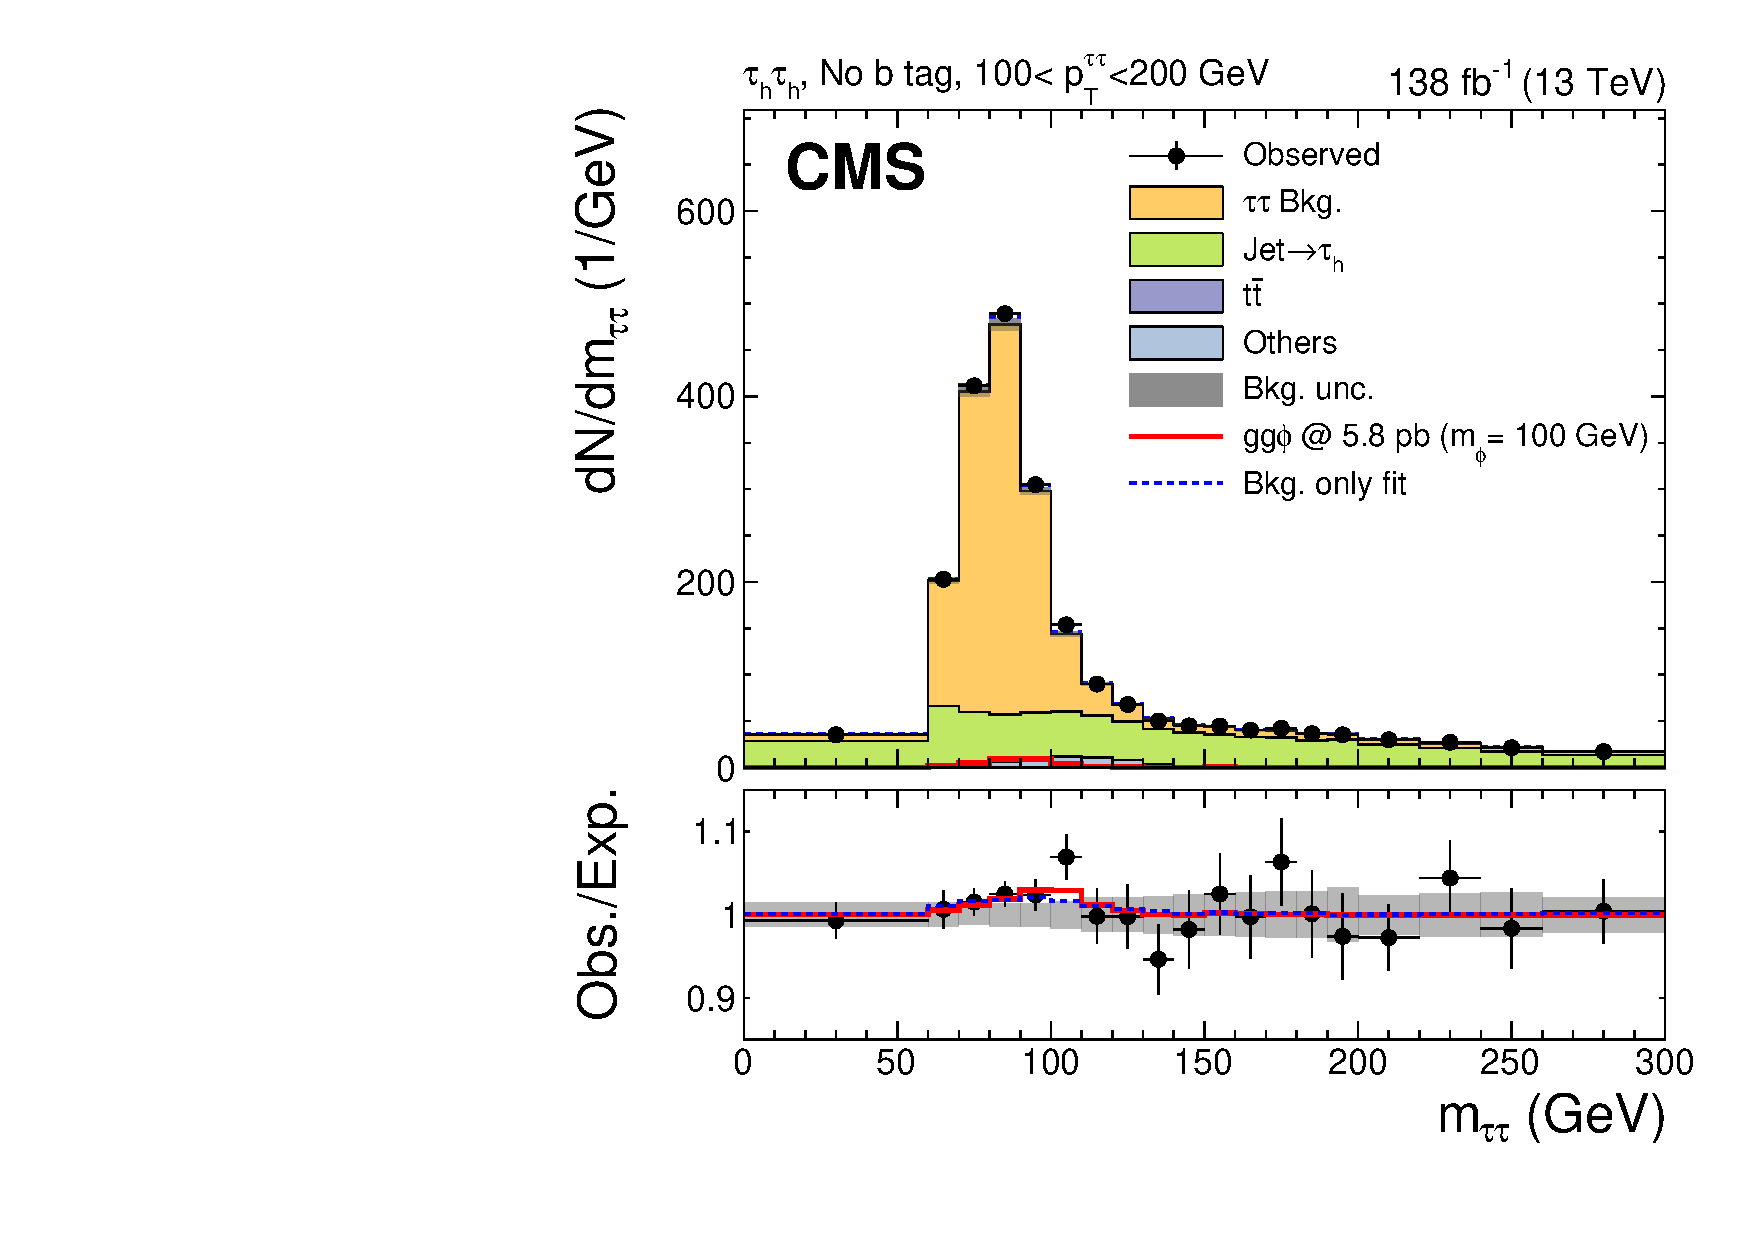
\includegraphics[width=0.4\textwidth]{Figures/postfit_lowmass_tt_nobtag_mediumpT.pdf}}
    \subfloat[]{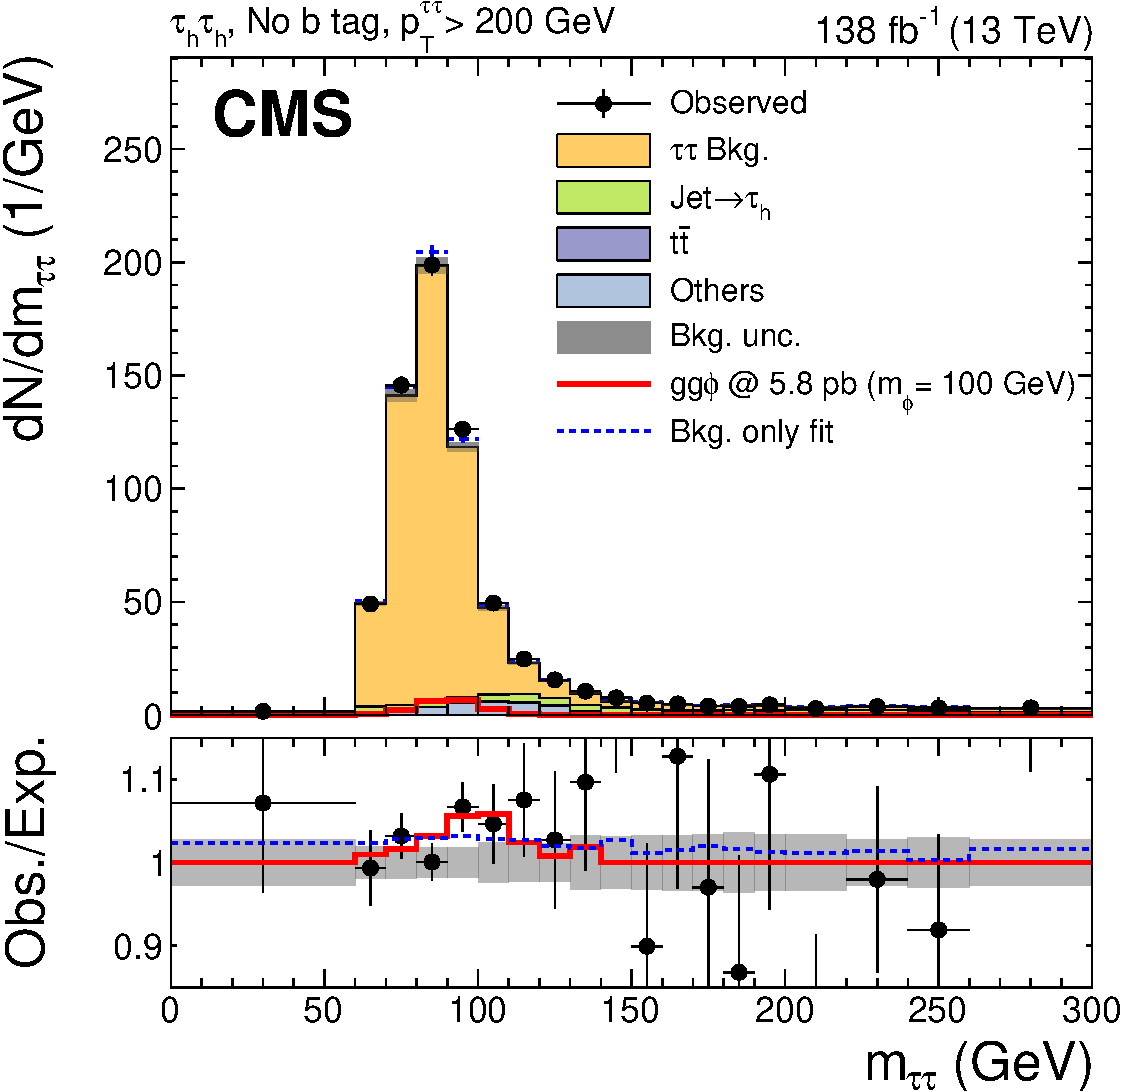
\includegraphics[width=0.4\textwidth]{Figures/postfit_lowmass_tt_nobtag_highpT-cropped.pdf}} \\
    \subfloat[]{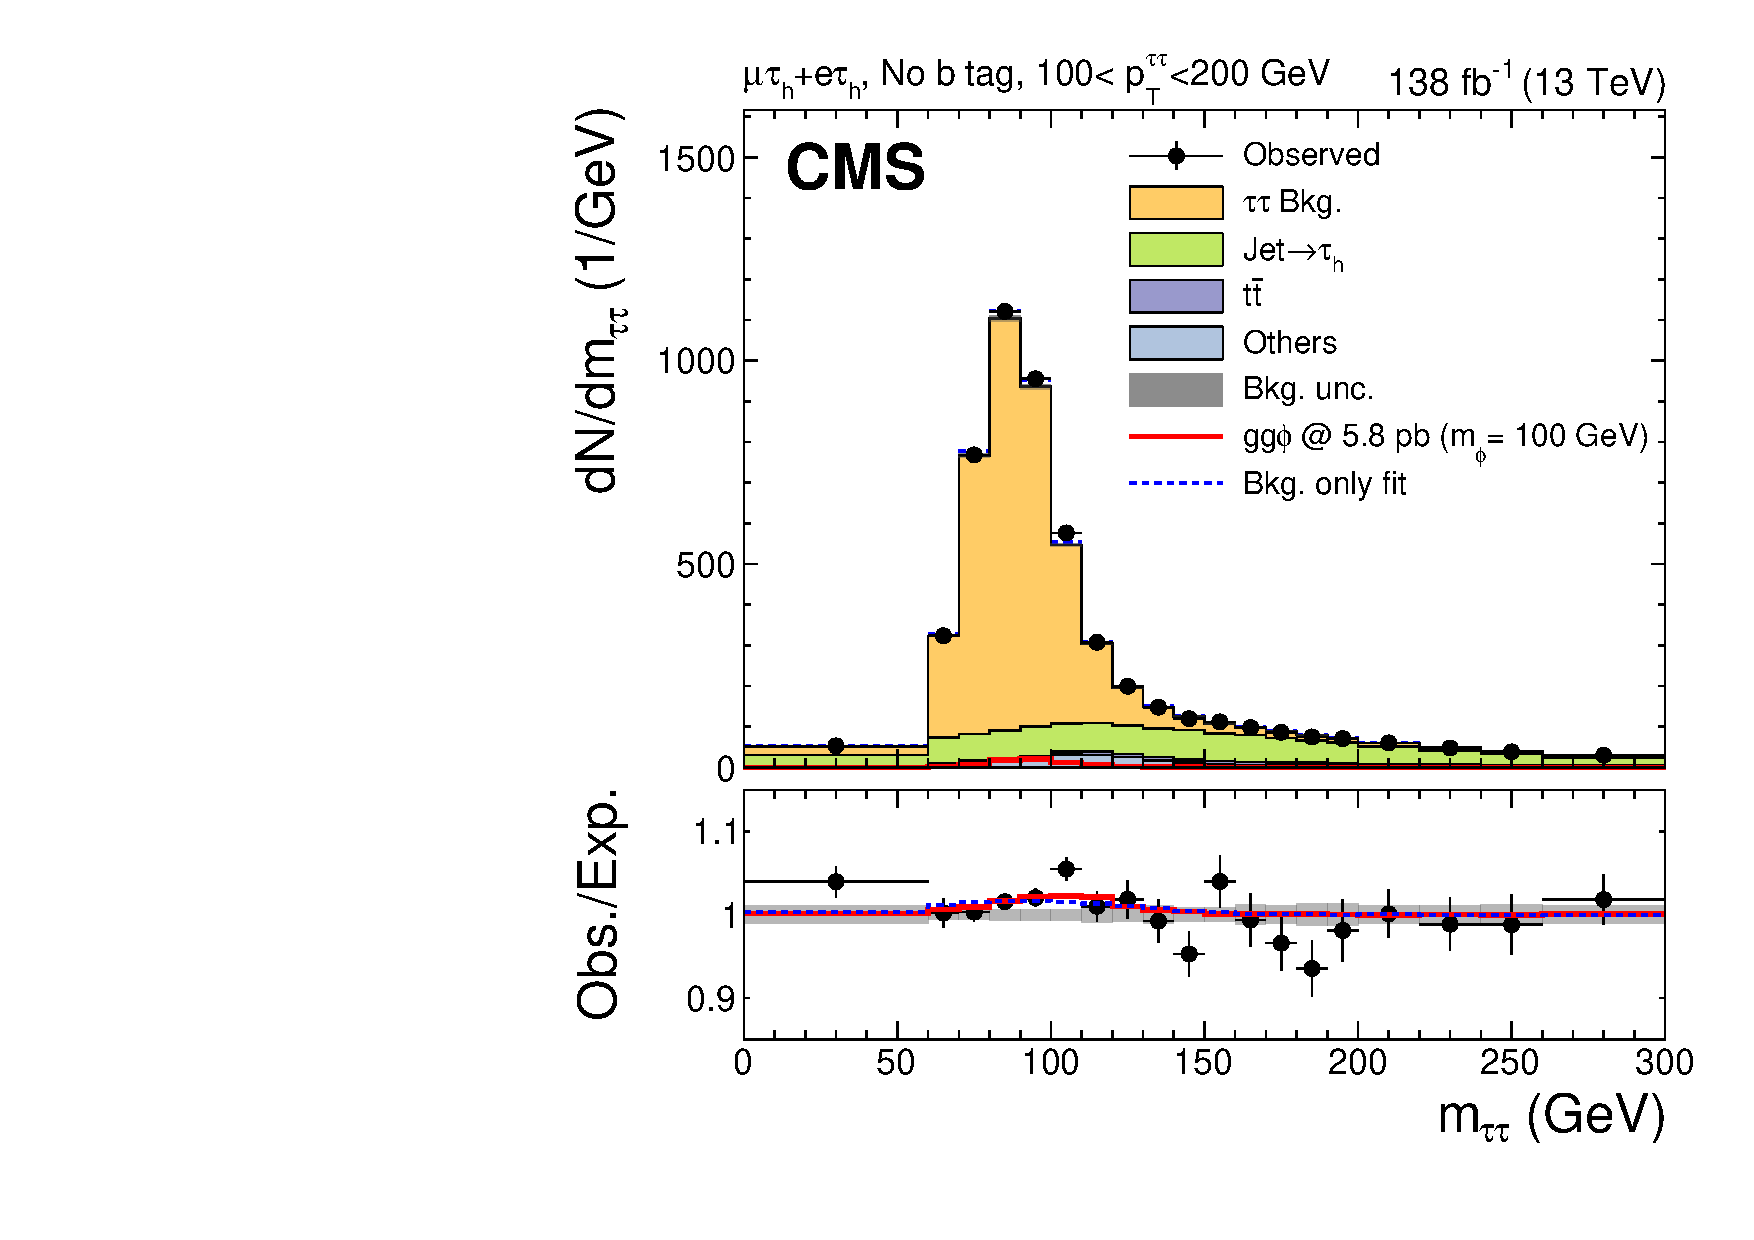
\includegraphics[width=0.4\textwidth]{Figures/postfit_lowmass_lt_nobtag_mediumpT.pdf}}
    \subfloat[]{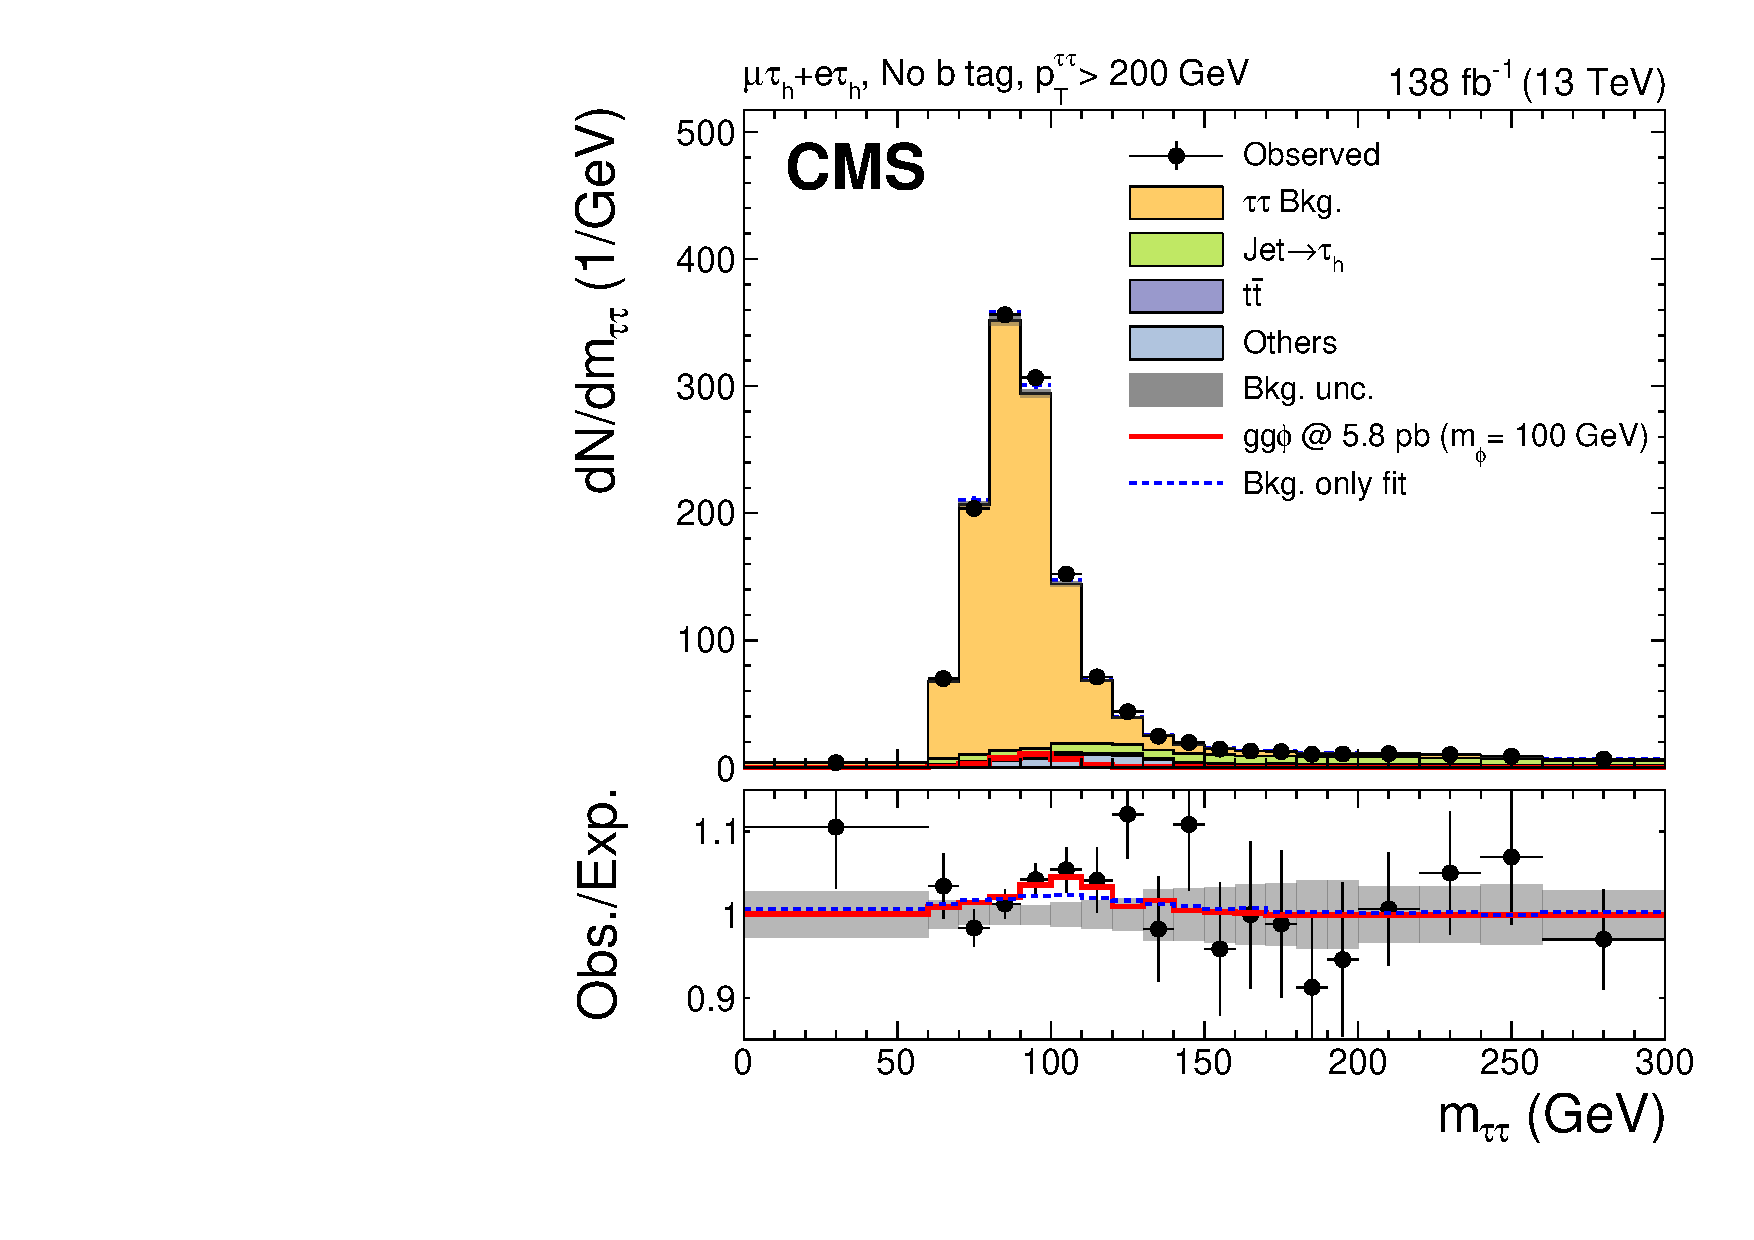
\includegraphics[width=0.4\textwidth]{Figures/postfit_lowmass_lt_nobtag_highpT.pdf}} \\
    \subfloat[]{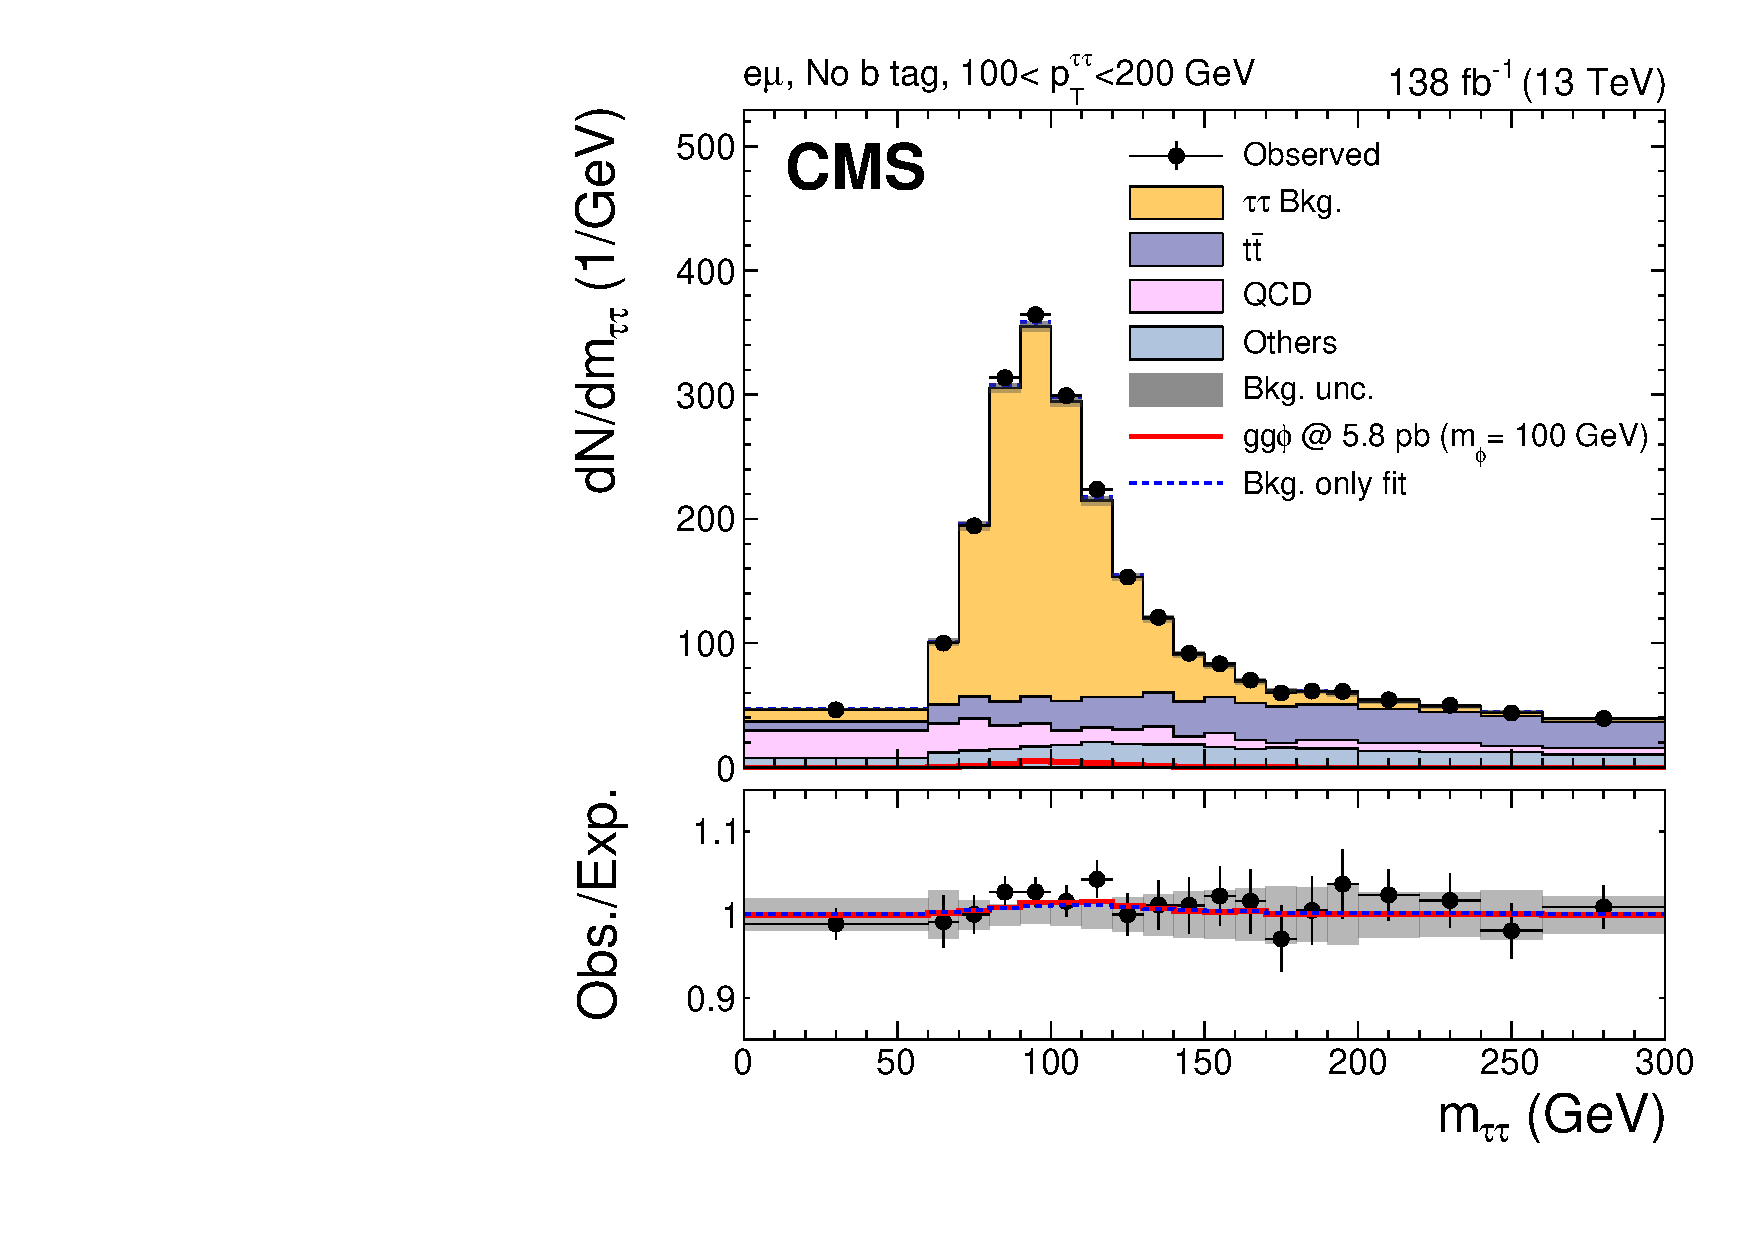
\includegraphics[width=0.4\textwidth]{Figures/postfit_lowmass_em_nobtag_mediumpT.pdf}}
    \subfloat[]{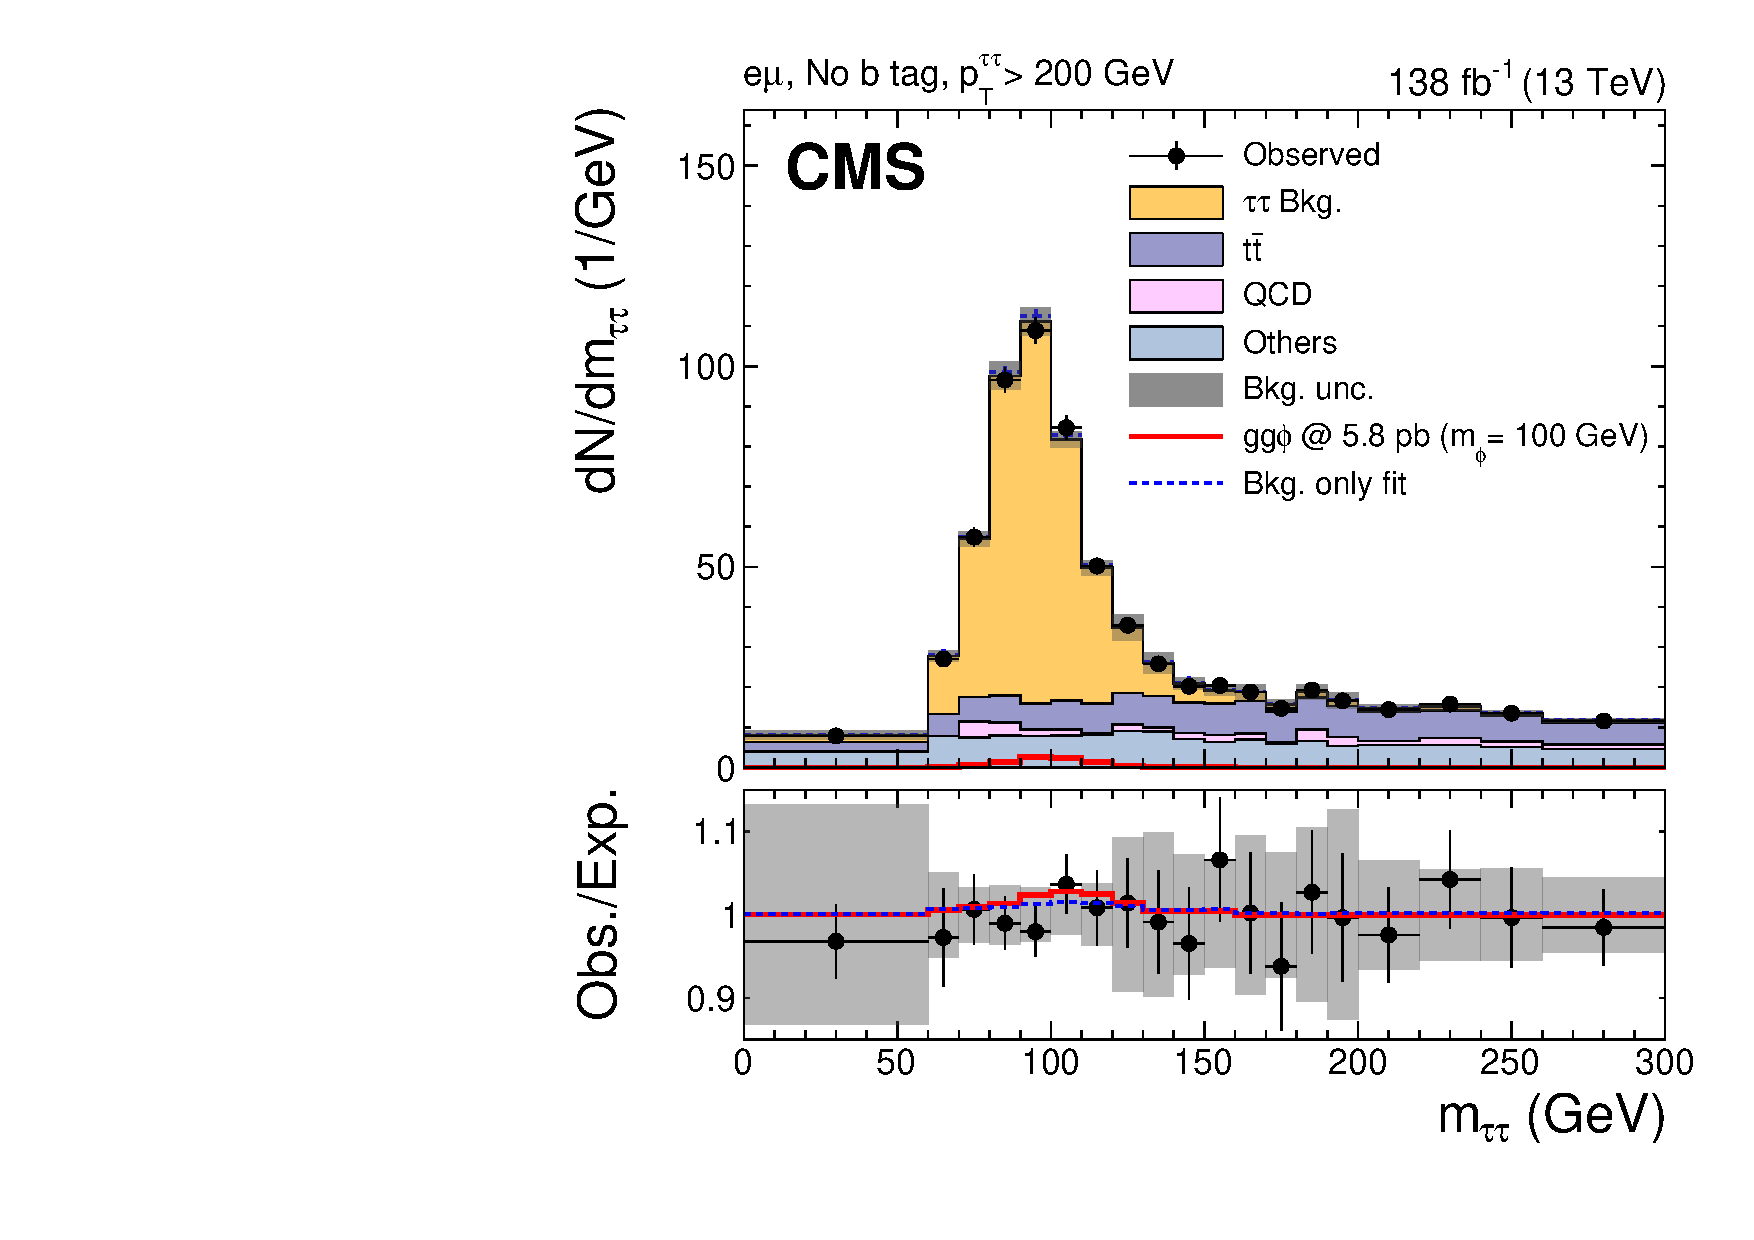
\includegraphics[width=0.4\textwidth]{Figures/postfit_lowmass_em_nobtag_highpT.pdf}}
\caption[Plots of the $m_{\tau\tau}$ distributions in the low-mass optimisation categories.]{Distributions of $m_{\tau\tau}$ in the no b tag second highest (a, c and e) and highest (b, d and e) $\pT$ category for the $\tauhtauh$ (a and b), the combined $\etauh$ and $\mutauh$ (c and d) and the $\emu$ (d and e) channels. The solid histograms show the stacked background predictions after a signal-plus-background fit to the data. The best-fit gluon fusion signal for $m_{\phi}$ = 100 GeV is shown by the red line. Also shown by a blue dashed line on the bottom pad is the ratio of the background predictions for the background-only fit to the signal-plus-background fit~\cite{CMS:2022rbd}. }
\label{fig:low_mass_postfit}
\end{figure}

\begin{figure}[!hbtp]
\centering
    \subfloat[]{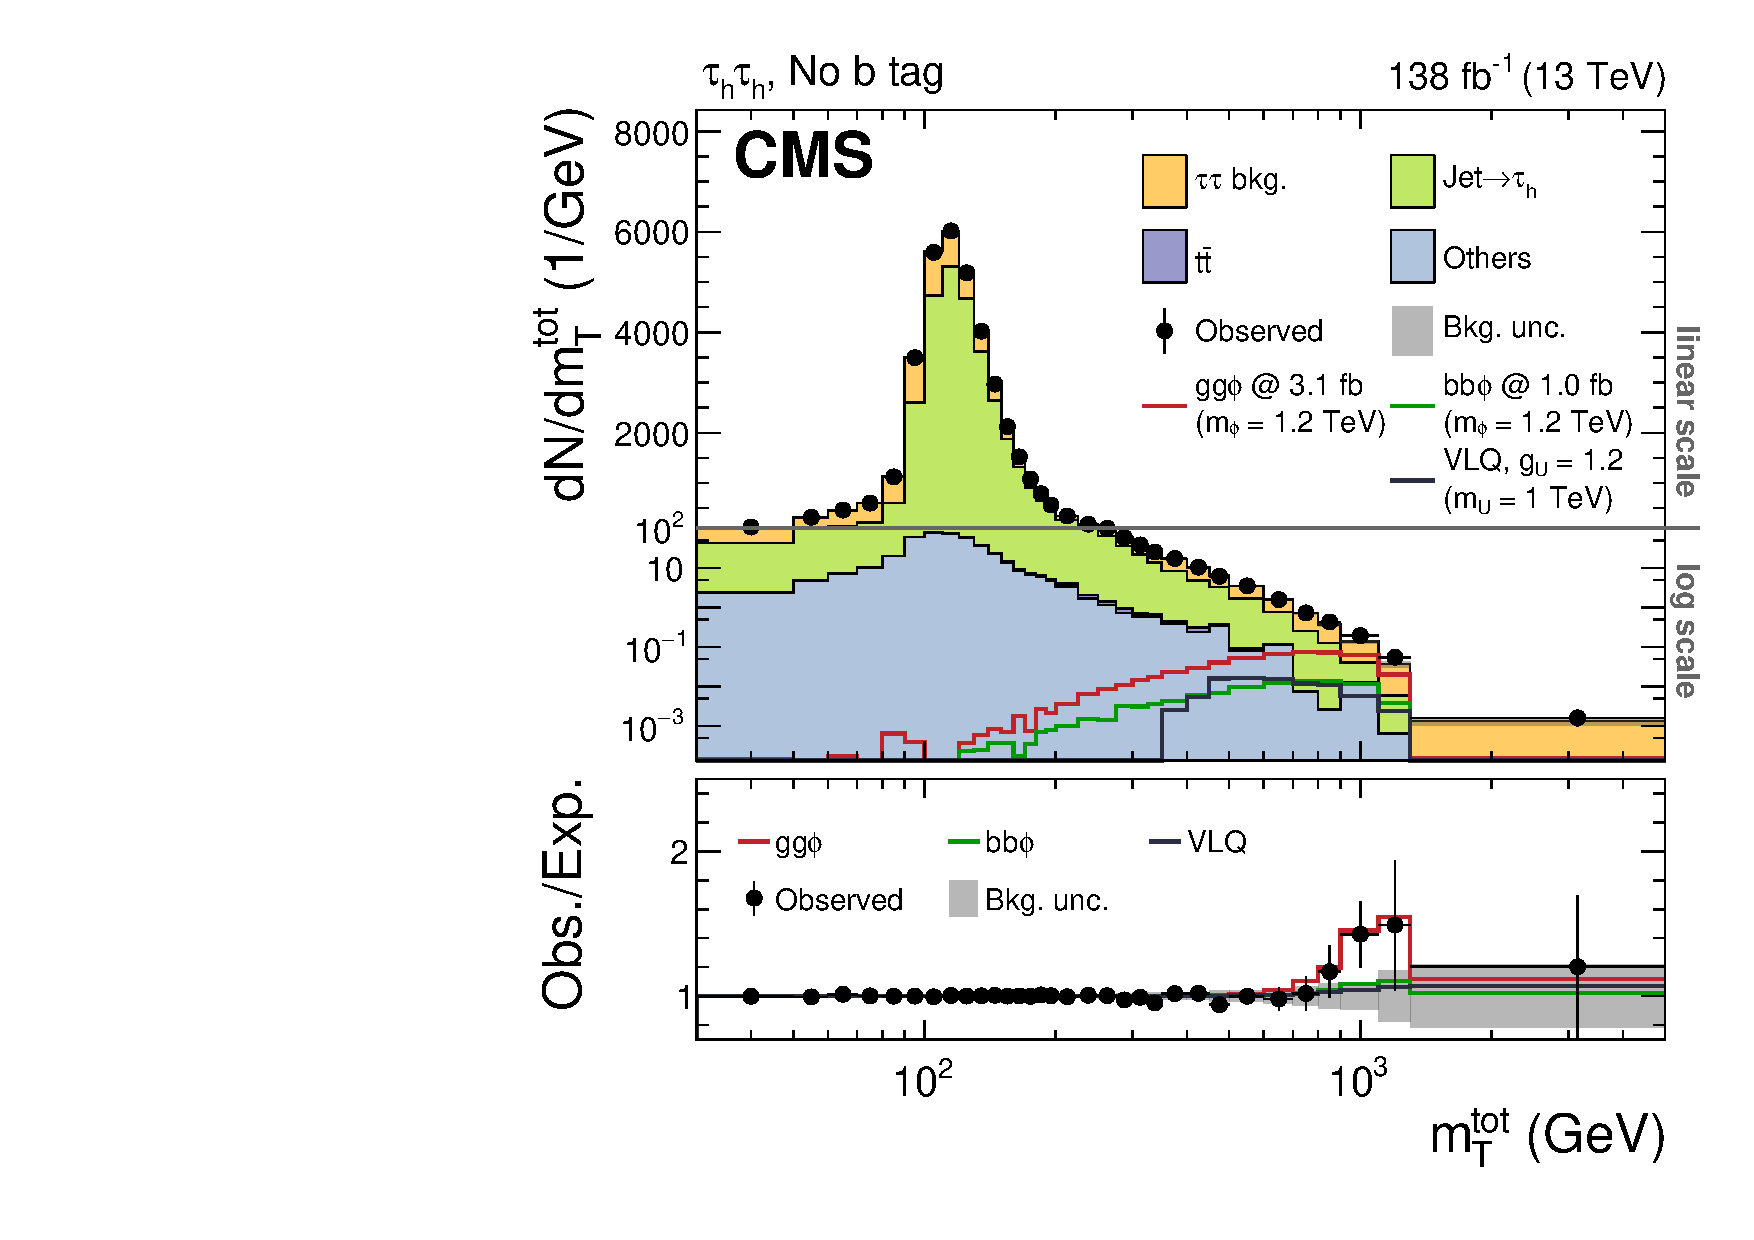
\includegraphics[width=0.42\textwidth]{Figures/postfit_highmass_tt_nobtag.pdf}}
    \subfloat[]{\includegraphics[width=0.42\textwidth]{Figures/postfit_highmass_tt_btag.pdf}} \\
    \subfloat[]{\includegraphics[width=0.42\textwidth]{Figures/postfit_highmass_lt_nobtag_tightmT.pdf}}
    \subfloat[]{\includegraphics[width=0.42\textwidth]{Figures/postfit_highmass_lt_btag_tightmT.pdf}} \\
    \subfloat[]{\includegraphics[width=0.42\textwidth]{Figures/postfit_highmass_em_nobtag_mediumdzeta.pdf}}
    \subfloat[]{\includegraphics[width=0.42\textwidth]{Figures/postfit_highmass_em_btag_mediumdzeta.pdf}}
\caption[Plots of the $m_{T}^\text{tot}$ distributions in the high-mass optimisation categories.]{Distributions of $m_{T}^\text{tot}$ in the $\tauhtauh$ no b tag (a) and b tag (b) categories, the combined $\etauh$ and $\mutauh$ no b tag (c) and b tag (d) \texttt{Tight-$m_{T}$} categories and the $\emu$ no b tag (e) and b tag (f) \texttt{Medium-$D_{\zeta}$} categories. The solid histograms show the stacked background predictions after a background-only fit to the data. The best-fit gluon fusion signal for $m_{\phi}$ = 1.2 TeV is shown by the red line, b-associated production and $U_{1}$ signals are also shown for illustrative purposes~\cite{CMS:2022rbd}.}
\label{fig:high_mass_postfit}
\end{figure}

\section{Model-independent results}

\subsection{Limits}

95\% \ac{CL} limits are set on the assumption of the absence of a signal for the search for a gg$\phi$ or bb$\phi$ resonance and these are shown in Figure~\ref{fig:model_independent_limits}.
In each case, the other process is allowed to float freely in the fit.
The excesses observed in the postfit distributions act to weaken the observed limit compared to the expected limit at 100 GeV and 1.2 TeV, as more data was observed than expected.
For gg$\phi$ production, the expected limits flatten under 100 GeV, due to the difficulty of separating the signal from the Z boson at this mass.
Both sets of limits vary from $\mathcal{O}(10\text{ pb})$ at 60 GeV to $0.3$ fb at 3.5 TeV. \\

\begin{figure}[!hbtp]
\centering
    \subfloat[]{\includegraphics[width=0.65\textwidth]{Figures/model_independent_limit_ggH.pdf}} \\
    \subfloat[]{\includegraphics[width=0.65\textwidth]{Figures/model_independent_limit_bbH.pdf}}
\caption[Plots of the model-independent limits on the cross-sections of gluon fusion and b-associated production multiplied by the $\tau\tau$ branching fraction.]{Expected (dashed line) and observed (solid line and dots) 95\% CL upper limits on the product of the cross-sections and branching fraction for the decay into $\tau$ leptons for gg$\phi$ (a) and bb$\phi$ (b) production in a mass range of 60 $\leq m_{\phi} \leq$ 3500 GeV.  The dark green and bright yellow bands indicate the central 68\% and 95\% intervals for the expected exclusion limit~\cite{CMS:2022rbd}.}
\label{fig:model_independent_limits}
\end{figure}

95\% \ac{CL} expected limits are drawn on the fit to each di-$\tau$ decay channel individually and are shown in Figure~\ref{fig:model_independent_limits_by_channel}.
This gives a measure of the sensitivity of each channel.
In the high-mass optimisation categories, the combined limit is heavily dominated by the $\tauhtauh$ channel.
This is mostly driven by the branching fractions, as all channels in this mass range have similar signal separation ability.
In the high-mass optimisation categories, the combined limit is more a contribution of all channels. 
In the $\tauhtauh$ channel in this region, the \ac{QCD} multijet background is the largest fraction of any non $Z\rightarrow\tau\tau$ backgrounds in all channels and so the limit for this channel is weakened and the other channels contribute to the combined limit more.
The high double-$\tau_h$ trigger $\pT$ thresholds (chosen because of the \ac{QCD} multijet background) also lowers the signal acceptance in the $\tauhtauh$ channel. \\

\begin{figure}[!hbtp]
\centering
    \subfloat[]{\includegraphics[width=0.5\textwidth]{Figures/limit_comparison_mssm_ggphi.pdf}}
    \subfloat[]{\includegraphics[width=0.5\textwidth]{Figures/limit_comparison_mssm_bbphi.pdf}}
\caption[Plots of the expected model-independent limits split by the $\tau\tau$ decay channels.]{Comparison of the expected 95\% CL upper limits on the product of the cross-sections and branching fraction for the decay into $\tau$ leptons for gg$\phi$ (a) and bb$\phi$ (b) production, split by the $\tau\tau$ decay products fit individually.}
\label{fig:model_independent_limits_by_channel}
\end{figure}

A comparison of the limits is also made with the ATLAS experiment and in particular the results presented in Reference~\cite{ATLAS:2020zms}.
This ATLAS search looks for the same signal but over a smaller mass range, from 200 GeV to 2.5 TeV.
Plots showing the comparison of the expected and observed limits for gg$\phi$ and bb$\phi$ are shown in Figure~\ref{fig:model_independent_limits_ATLAS}.
The expected limits from the \ac{CMS} and ATLAS results are roughly compatible over the shared mass range, except at high mass where the extra statistics from the embedded genuine di-$\tau$ samples compared to \ac{MC} allow for lower background uncertainties and hence a stronger limit.
The ATLAS result observed no excess of events compatible with a gg$\phi$ signal at 1.2 TeV, in fact, a small deficit was observed.
Also, ATLAS observed local excesses at 400 GeV of 2.2$\sigma$ for gg$\phi$ and 2.7$\sigma$ for bb$\phi$.
None of these excesses are consistent between the ATLAS and \ac{CMS} results.
The ATLAS search does not stretch to the mass of the low mass \ac{CMS} excess and so cannot be used as a cross-check for this.

\begin{figure}[!hbtp]
\centering
    \subfloat[]{\includegraphics[width=0.5\textwidth]{Figures/limit_comparison_gg_ATLAS.pdf}}
    \subfloat[]{\includegraphics[width=0.5\textwidth]{Figures/limit_comparison_bb_ATLAS.pdf}}
\caption[Plots of the comparison of the model-independent limits between CMS and ATLAS.]{Comparison of the expected 95\% CL upper limits on the product of the cross-sections and branching fraction for the decay into $\tau$ leptons for gg$\phi$ (a) and bb$\phi$ (b) production, split by the CMS result detailed in this thesis and the ATLAS result from Reference~\cite{ATLAS:2020zms}.}
\label{fig:model_independent_limits_ATLAS}
\end{figure}

\subsection{Significance and compatibility}
\label{sec:sig_and_compat}

The $p$-values and significances at each model-independent signal hypothesis are calculated as described in Section~\ref{sec:sig_ext} and shown in Figure~\ref{fig:significance}.
Identical to the model-independent limits, the gg$\phi$ or bb$\phi$ process is allowed to float freely if not the parameter of interest.
The excesses for the gg$\phi$ process peak at 100 GeV and 1.2 TeV and quantify to a local (global) significance of 3.1$\sigma$ (2.7$\sigma$) and 2.8$\sigma$ (2.2$\sigma$) respectively.
There are also excesses at neighbouring mass points (particularly at high mass), however, this is consistent with the mass resolution of the fitted templates for the central values.
No deviations beyond 2$\sigma$ are observed for bb$\phi$ production. \\

\begin{figure}[!hbtp]
\centering
    \subfloat[]{\includegraphics[width=0.5\textwidth]{Figures/significance_plot_ggH.pdf}}
    \subfloat[]{\includegraphics[width=0.5\textwidth]{Figures/significance_plot_bbH.pdf}}
\caption[Plots of the local $p$-value and significance for gluon fusion and b-associated production.]{Local $p$-value and significance of a gg$\phi$ (a) and bb$\phi$ (b) signal as a function of $m_{\phi}$~\cite{CMS:2022rbd}.}
\label{fig:significance}
\end{figure}

As many different decay channels and categories are used to extract these significances, the signal strength is studied in each channel and category.
This is done via compatibility fits as described in Section~\ref{sec:sig_ext}, where the signal strength parameter in each channel/category is decoupled.
No statistically significant differences are observed in the best-fit signal strength in any decay channel or category fit and $p$-values between each channel or category fit are always above 0.05.
Figure~\ref{fig:low_mass_compatibility} shows the results of the compatibility fits in the low-mass optimisation categories split by di-$\tau$ decay channels and the $\pT$ bins fit. 
Figure~\ref{fig:high_mass_compatibility} shows the compatibility fits in the high-mass optimisation categories split by di-$\tau$ decay channels.
The low-mass signal strengths are no more dominant in any $\pT$ region than another.
In both low- and high-mass cases, the signal strengths are consistent across di-$\tau$ decay channels.
There is a small shift in the high mass $\emu$ categories to a negative signal strength, these categories have little to no sensitivity to this signal in comparison to others and a small deficit is observed in data, resulting in fits for a negative signal strength with a large uncertainty. 


\begin{figure}[!hbtp]
\centering
    \subfloat[]{\includegraphics[width=0.5\textwidth]{Figures/ChannelCompatibilityCheck_FitResults_mH100_channel.pdf}}
    \subfloat[]{\includegraphics[width=0.5\textwidth]{Figures/ChannelCompatibilityCheck_FitResults_mH100_cat.pdf}}
\caption[Plots of the compatibility of the 100 GeV excess across the channels and categories.]{Compatibility plots of the 100 GeV excess split into analysis channels (a) and categories (b). In each case, the fitted signal strength is decoupled in the bin shown on the plot~\cite{CMS:2022rbd}.}
\label{fig:low_mass_compatibility}
\end{figure}

\begin{figure}[!hbtp]
\centering
    \includegraphics[width=0.5\textwidth]{Figures/ccc_fit_result_mH1200_per-channel.pdf}
\caption[Plots of the compatibility of the 1.2 TeV excess across the channels.]{Compatibility plots of the 1.2 TeV excess split by analysis channels. In each case, the fitted signal strength is decoupled in each channel~\cite{CMS:2022rbd}.}
\label{fig:high_mass_compatibility}
\end{figure}

\subsection{2D likelihood scans}

As the model-independent search looks for two signal modes at each mass point, the results for both processes happening simultaneously are studied.
This is done in the form of two-dimensional likelihood scans.
The best-fit cross-section times branching fractions of each process and the 95\% and 68\% confidence intervals are shown for a number of different mass scenarios in Figure~\ref{fig:2d_likelihood_scans}.
The \ac{SM} prediction in all plots is at (0,0).
These results highlight how the excesses at 100 GeV and 1.2 TeV are dominated in the phase space in which gg$\phi$ and not bb$\phi$ signals are allowed.
In the 60 GeV example, there are smaller deviations in both gg$\phi$ and bb$\phi$ and the SM background is again over 2$\sigma$ away.
Otherwise, signal strengths are completely compatible with the background expectation.


\begin{figure}[!hbtp]
\centering
    \subfloat[]{\includegraphics[width=0.33\textwidth]{Figures/2d_lkld_60.pdf}}
    \subfloat[]{\includegraphics[width=0.33\textwidth]{Figures/2d_lkld_100.pdf}}
    \subfloat[]{\includegraphics[width=0.33\textwidth]{Figures/2d_lkld_125.pdf}} \\
    \subfloat[]{\includegraphics[width=0.33\textwidth]{Figures/2d_lkld_160.pdf}}
    \subfloat[]{\includegraphics[width=0.33\textwidth]{Figures/2d_lkld_250.pdf}}
    \subfloat[]{\includegraphics[width=0.33\textwidth]{Figures/2d_lkld_500.pdf}} \\
    \subfloat[]{\includegraphics[width=0.33\textwidth]{Figures/2d_lkld_1000.pdf}}
    \subfloat[]{\includegraphics[width=0.33\textwidth]{Figures/2d_lkld_1200.pdf}}
    \subfloat[]{\includegraphics[width=0.33\textwidth]{Figures/2d_lkld_3500.pdf}}
\caption[Plots of the maximum likelihood scans for the model-independent search.]{Maximum likelihood scans, including 68\% and 95\% CL contours obtained from the signal likelihood for the model-independent search. The scans are shown for$m_{\phi}$ values of 60 (a), 100 (b), 125 (c), 160 (d), 250 (e), 500 (f), 1000 (g), 1200 (h) and 3500 (i) GeV~\cite{CMS:2022rbd}.}
\label{fig:2d_likelihood_scans}
\end{figure}

\section{Model-dependent limits}

The exclusion contours for two benchmark scenarios of the \ac{MSSM}, $M_{h}^{125}$ and $M_{h,EFT}^{125}$, are presented in Figure~\ref{fig:mssm_limits}. 
The red hatched regions denote areas where $m_{h}$ is inconsistent with the observed \ac{SM} Higgs boson mass within a ${\pm}3$ GeV boundary. 
For low values of $\tan\beta$, higher values of the additional SUSY particle masses, denoted as $m_{\text{SUSY}}$, are needed to explain a mass of approximately $125$ GeV for the Higgs boson. 
In the $M_{h}^{125}$ scenario, $m_{\text{SUSY}}$ is fixed, and the predicted value of $m_{h}$ is below $122$ GeV. 
In contrast, the $M_{h,EFT}^{125}$ scenario adjusts $m_{\text{SUSY}}$ to satisfy the required value of $m_{h}$ for each point in $m_{A}$ and $\tan\beta$ individually, accounting for the logarithmic corrections associated with the large values of $m_{\text{SUSY}}$ using an effective field theory approach. 
The red hatched region in Figure~\ref{fig:mssm_limits}b indicates that the required values of $m_{\text{SUSY}}$ exceed the GUT scale at very low values of $m_{A}$ in this scenario. 
The Higgs boson masses, mixing angle $\alpha$, and effective Yukawa couplings were calculated using \textsc{FeynHiggs}, and branching fractions for the decay into $\tau$ leptons and other final states were obtained from a combination of the \textsc{FeynHiggs} and \textsc{HDECAY}, following the prescriptions in References~\cite{LHCHiggsCrossSectionWorkingGroup:2013rie,deFlorian:2016spz,Denner:2011mq}, for the scenarios described in Reference~\cite{Bagnaschi:2791954}. \\

For the $M_{h,EFT}^{125}$ scenario, the sensitivity sharply drops at $m_{A}=2m_{t}$ due to a drop in the branching fractions for the decay of A and H into $\tau$ leptons, when the A and H decay into two on-shell t quarks becomes kinematically accessible. 
Both scenarios are excluded at 95\% CL for $m_{A}\lesssim350$ GeV. 
For $m_{A}\lesssim250$ GeV, most of the ggH/A events do not enter the no b tag categories due to the $m_{\tau\tau}>250$ GeV requirement. 
In this parameter space, the sensitivity to the \ac{MSSM} is driven by the measurements of the observed Higgs boson, even though H and A still contribute to the categories here. 
The sensitivity to the H and A enters mainly via the bb$\phi$ signal in the b tag categories, especially for increasing values of $\tan\beta$. \\

Other \ac{MSSM} scenarios are tested and detailed in Reference~\cite{CMS:2022rbd}.
One scenario of note is the $M_{H}^{125}$ scenario, which is the equivalent scenario to the $M_{h}^{125}$ but with the observed Higgs boson being the heavier \ac{CP}-even Higgs boson.
Despite the local excess at a resonant mass of 100 GeV, this scenario is entirely excluded by the search. 
This is mostly due to the sensitivity of the b tag categories to b-associated production.
The local excess observed at 1.2 TeV is hard to rectify within these \ac{MSSM} benchmark scenarios.
The lack of any excess in the b tag categories strictly constrains the b-associated production cross-section times the branching fractions.
It is not possible within these scenarios to predict the excess of gluon fusion events within the constraints placed on b-associated production. \\

\begin{figure}[!hbtp]
\centering
    \subfloat[]{\includegraphics[width=0.65\textwidth]{Figures/model-dependent_limit_mh125.pdf}} \\
    \subfloat[]{\includegraphics[width=0.65\textwidth]{Figures/model-dependent_limit_mh125EFT.pdf}}
\caption[Plots of the model-dependent limits in MSSM benchamrk scenarios.]{Expected and observed 95\% CL exclusion contours in the MSSM $M_{h}^{125}$ (a) and $M_{h,EFT}^{125}$ (b) scenarios. The exclusion limit only on background expectation is shown as a dashed black line, the dark and bright grey bands show the 68\% and 95\% intervals of the expected exclusion and the observed exclusion contour is shown by the blue area. The parameter space where $m_{h}$ deviates by more than $\pm$3  GeV from the observed SM Higgs boson mass is shown by a red-hatched area.~\cite{CMS:2022rbd}
}
\label{fig:mssm_limits}
\end{figure}

Upper limits of 95\% \ac{CL} for VLQ BM 1 and 2 are shown in Figure~\ref{fig:vlq_limits}. 
These are drawn with respect to the leptoquark mass ($m_{U}$) and coupling ($g_{U}$).
The limit on $g_{U}$ decreases as $m_{U}$ increases, with values of $g_U$ ranging from 1.3 to 5.2 in VLQ BM 1 and 0.8 to 3.2 in VLQ BM 2. 
VLQ BM 2 has stronger exclusion limits than VLQ BM 1 due to additional right-handed couplings of the leptoquark with a b quark and a $\tau$ lepton. \\

\begin{figure}[!hbtp]
\centering
    \subfloat[]{\includegraphics[width=0.65\textwidth]{Figures/vlq_bm_1.pdf}} \\
    \subfloat[]{\includegraphics[width=0.65\textwidth]{Figures/vlq_bm_2.pdf}}
\caption[Plots of the model-dependent limits in the vector leptoquark phase space.]{Expected and observed 95\% CL upper limits on $g_U$ in the VLQ BM 1 (a) and 2 (b) scenarios, in a mass range of $1<m_{U}<5$ TeV.  The exclusion limit only on that background expectation is shown as a dashed black line, the dark and bright grey bands show the 68\% and 95\% intervals of the expected exclusion and the observed exclusion contour is shown by the blue area. The 95\% confidence interval for the preferred region from the global fit presented in Reference~\cite{Cornella:2021sby} is also shown by the green shaded area~\cite{CMS:2022rbd}.}
\label{fig:vlq_limits}
\end{figure}

The observed limits fall within the central 95\% intervals of the expected limits when no signal is present. 
The expected limits are also within the 95\% confidence interval of the best fit results reported by Reference~\cite{Cornella:2021sby} and described in Section~\ref{sec:b_anomalies}.
This indicates that the search is capable of detecting a part of the parameter space that can explain the anomalies observed in B physics and since no significant excess was observed in this search, new constraints are placed on the vector leptoquark phase space.
Similarly to the \ac{MSSM} scenarios, the local excess at 1.2 TeV is not consistent with a VLQ BM 1 or 2 vector leptoquark.
Again this is due to the lack of signal in the b tag categories, where the reduction in backgrounds makes the t-channel signal with initial state radiation the dominant search option.



%\newpage
%\chapter{\texorpdfstring{Search for New Physics in $\tau^+\tau^-\tau^+\tau^-$ Final States}{Search for new physics in tautautautau final states}}
\label{sec:H_A_to_4_tau_analysis}

Enhancement from $\tan\beta$ to up or down-like quark couplings to additional Higgs bosons are essential for the majority of searches for extended Higgs sectors, including in the analysis detailed in Chapter~\ref{sec:bsm_H_to_tau_tau_analysis}.
However, in some \ac{2HDM}s it can be the case that both up and down-like couplings to additional Higgs bosons are suppressed and this parameter space is left relatively untouched by \say{\ac{MSSM}-like} searches.
In particular, type X \ac{2HDM}s where only lepton couplings are enhanced by $\tan\beta$, allow for new physics loop contributions to \ac{SM} measurements through couplings between leptons and additional Higgs bosons.
This is particularly interesting in the context of the g-2 anomaly~\cite{Muong-2:2006rrc,Muong-2:2021ojo} with reasoning explained in Section~\ref{sec:gm2_anomaly}.
This chapter will detail a search for such an extended Higgs sector, that looks for a production mode not suppressed at high $\tan\beta$, through the process $Z^{*}\rightarrow \phi A \rightarrow 4\tau$.
This search is split up into two sections:

\begin{enumerate}[i)]
  \item A model independent search for the $Z^{*}\rightarrow \phi A \rightarrow 4\tau$ process. Both additional particles are required to have narrow width and no assumptions are made on the production cross-section via an off-shell Z boson or the branching fraction of $\phi$ and A decaying to a pair of tau leptons.
   \item A search for the type X \ac{2HDM}, motivated by the phase space for possible explanations to the g-2 anomaly. The $m_{A}$-$\tan\beta$ phase space for scenarios of $m_\phi$ in the alignment limit is scanned, as well as checks outside of this limit on the $\cos(\beta-\alpha)$-$\tan\beta$ for specific scenarios of both $m_\phi$ and $m_A$.
\end{enumerate}

These searches are performed with the full run-2 dataset ($138 \sifb$) collected by the \ac{CMS} experiment. 

\section{Signal Modelling}
\label{sec:4tau_signal_modelling}

Any additional Higgs boson produced in the type X \ac{2HDM} at high $\tan\beta$ will predominantly decay to tau leptons.
To probe the type X \ac{2HDM} at high $\tan\beta$, a production process that is not suppressed is required.
Reference~\cite{Jueid:2021avn} discusses that the following production modes of two additional Higgs bosons are dominant to produce any of these new particles at high $\tan\beta$:
\begin{enumerate}[i)]
  \item $pp \rightarrow Z^{*} \rightarrow \phi A \rightarrow (\tau^{-}\tau^{+})(\tau^{-}\tau^{+})$
  \item $pp \rightarrow Z^{*} \rightarrow H^{+}H^{-} \rightarrow (\tau^{-}\nu)(\tau^{+}\nu)$
  \item $pp \rightarrow W^{\pm *} \rightarrow H^{\pm}A \rightarrow (\tau^{\pm}\nu)(\tau^{-}\tau^{+})$
  \item $pp \rightarrow W^{\pm *} \rightarrow H^{\pm}\phi \rightarrow (\tau^{\pm}\nu)(\tau^{-}\tau^{+})$
\end{enumerate}
As the production cross sections are of the similar magnitudes, the search sensitivities depend on the separation of the signals from background.
In general, the more objects you can select in the final state, the smaller the background contributions.
This is certainly true in tau enriched final states, where backgrounds can be dominated jets misidentified as hadronic taus and so every extra tau selected reduces this background.
In particular, (ii) has the production cross sections~\cite{Jueid:2021avn} far smaller than the observed limit for gluon fusion production of a single resonance shown in Figure~\ref{fig:model_independent_limits}(a) and it is not possible to use tau decay product and \ac{MET} alignment to separate the background, so does seem not a viable search option with the run-2 \ac{CMS} dataset.
The increased background from fewer object selections and looser charge sum selection on (iii) and (iv), makes (i) the golden search channel for a type X \ac{2HDM}. 
A Feynman diagram for this process is shown in Figure~\ref{fig:4tau_feynamn}. \\

\begin{figure}[H]
\centering
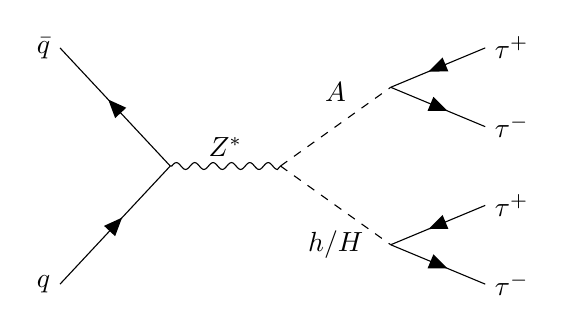
\begin{tikzpicture}[scale=2]
  \begin{feynman}
    \vertex [label=left:$q$] (a1) at (0,-0.25);
    \vertex [label=left:$\bar{q}$] (a2) at (0,1.25);
    \vertex (b) at (0.7,0.5);
    \vertex [label=above:$Z^{*}$] (b1) at (1.05,0.5);    
    \vertex (c) at (1.4,0.5);
    \vertex [label=below:$h/H$] (d11) at (1.75,0.15);
    \vertex [label=above:$A$] (d12) at (1.75,0.85);
    \vertex (d1) at (2.1,0);
    \vertex (d2) at (2.1,1);
    \vertex [label=right:$\tau^-$] (e1) at (2.7,-0.25);
    \vertex [label=right:$\tau^+$] (e2) at (2.7,0.25);
    \vertex [label=right:$\tau^-$] (e3) at (2.7,0.75);
    \vertex [label=right:$\tau^+$] (e4) at (2.7,1.25);
    \diagram* {
      (a1) -- [fermion] (b),
      (b) -- [fermion] (a2),
      (b) -- [photon] (c),
      (c) -- [scalar] (d1),
      (c) -- [scalar] (d2),
      (d1) -- [fermion] (e1),
      (e2) -- [fermion] (d1),
      (d2) -- [fermion] (e3),
      (e4) -- [fermion] (d2),
    };
  \end{feynman}
\end{tikzpicture}
\vspace*{10mm}
\caption{Diagram of production of two additional neutral Higgs bosons from an off-shell Z boson and their decays to tau leptons.}
\label{fig:4tau_feynamn}
\end{figure}

Signal templates for the production of this process with a mass grid for $\phi$ and A between 100 to 300 and 60 to 160 GeV respectively are generated.
These mass ranges are motivated from the results in Table~\ref{tab:gm2region}.
The samples are simulated in the five \ac{FS} at \ac{NLO} precision using the \MGvATNLO v2.6.5 event generator~\cite{Alwall:2011uj}.
Generation is performed using the parton distribution function NNPDF3.1~\cite{Ball:2014uwa,Ball:2017nwa}, where the $\tau$ lepton decay, parton showering and hadronisation are all modelled with the \PYTHIA event generator with the \ac{PU} profile matched to data~\cite{Sirunyan:2019dfx,Sjostrand:2014zea}.
The events are then passed through the \texttt{GEANT4}-based \cite{Agostinelli:2002hh} simulation of the \ac{CMS} detector and reconstructed in the same way as data.
Generator level distributions of di-$\tau$ mass distributions from the decay of $\phi$ and A are shown in Figure~\ref{fig:4tau_gen_dist}.\\

\begin{figure}[!hbtp]
\centering
    \subfloat[]{\includegraphics[width=0.49\textwidth]{Figures/mA_dist.pdf}}
    \subfloat[]{\includegraphics[width=0.49\textwidth]{Figures/mphi_dist.pdf}} 
\caption{Generator level distributions of the visible mass densities for A (a) and $\phi$ (b) for the signal process.}
\label{fig:4tau_gen_dist}
\end{figure}

The cross sections in the alignment scenarios are also determined with this procedure and vary from 10 fb (highest $m_{A}$ and $m_{\phi}$ scenario) to 650 fb (lowest $m_{A}$ and $m_{\phi}$ scenario), as shown in Figure~\ref{fig:4tau_xs}.
These are independent of $\tan\beta$, however, out of the alignment scenarios the cross sections for H scales with $\sin^{2}(\beta-\alpha)$ and h scales with $\cos^{2}(\beta-\alpha)$. \\

\begin{figure}[!hbtp]
\centering
    \includegraphics[width=0.8\textwidth]{Figures/cross_sections.png}
\caption{Calculated productions cross sections for the $Z^{*} \rightarrow \phi A$ process, varying the masses of $\phi$ and A.}
\label{fig:4tau_xs}
\end{figure}

The branching fractions of $\phi$ and A to pairs of $\tau$ leptons is dependent on both $tan\beta$ and $\beta-\alpha$.
For this analysis, the branching fractions are calculated using \texttt{2HDECAY} \cite{Krause:2018wmo}.
In the alignment scenarios, the $A\rightarrow\tau\tau$ branching fractions are approximately 1 above $\tan\beta \approx 2$, where below they sharply drop off and other processes such as $A\rightarrow b\bar{b}$ become dominant.
This is also true for $\phi\rightarrow\tau\tau$ branching fractions, except in the case where $m_\phi$ is greater than $m_A$ by more than $m_Z$, and so the $\phi\rightarrow ZA$ decay becomes kinematically feasible and can dominate at high $\tan\beta$.
Examples of this are shown in Figure~\ref{fig:4tau_br_1d}.
Out of the alignment scenario, the branching fractions of $\phi$ to tau leptons becomes smaller as the magnitude of the coupling of additional neutral Higgs bosons to taus is reduced, whilst the $A$ branching fractions, like the couplings, are left unchanged.
An example of the $\phi$ branching fractions out of the alignment scenario is shown in Figure~\ref{fig:4tau_br_2d}.

\begin{figure}[!hbtp]
\centering
    \subfloat[]{\includegraphics[width=0.49\textwidth]{Figures/A_br_plot_mphi200.pdf}}
    \subfloat[]{\includegraphics[width=0.49\textwidth]{Figures/phi_br_plot_mphi200.pdf}} 
\caption{Calculated branching fractions of A (a) and $\phi$ (b) decaying to a pair of $\tau$ leptons for various mass scenarios.}
\label{fig:4tau_br_1d}
\end{figure}

\begin{figure}[!hbtp]
\centering
    \includegraphics[width=0.7\textwidth]{Figures/phi_branching_fractions_mphi200_mA160.pdf}
\caption{Calculated branching fractions in the $\cos(\beta-\alpha)$-$\tan\beta$ phase space for $\phi$ of mass 200 GeV decaying to a pair of $\tau$ leptons, in the scenario where $m_A = 160$ GeV.}
\label{fig:4tau_br_2d}
\end{figure}

\section{Event Selection}

In comparison to Chapter~\ref{sec:bsm_H_to_tau_tau_analysis}, four $\tau$ leptons produce a much larger number of possible final states. 
All variations of $e$, $\mu$ and $\tau_h$ final state combinations and their branching fractions are shown in Table~\ref{tab:4tau_bf}.
Just under 90\% of the branching ratio goes to decay products containing two or more hadronic taus.
These are the main final states that are explored in this analysis. 
In addition to this, an orthogonal $\tau_h \tau_h \tau_h$ channel is added to target events where reconstruction of the $\tau_h \tau_h \tau_h \tau_h$ channel loses a single $\tau_h$ object.
This can come about due to low triggering and ID efficiency of $\tau_h$ candidates, as well as the high $\pT$ thresholds required for both. \\
In total, the analysis consists of 7 channels.

\begin{table}[H]
    \centering
    \begin{tabular}{|c|c|}
         \hline
         Channel & Branching Fraction  \\
         \hline
         \hline
         $e \tau_h \tau_h \tau_h$ & 19.4\% \\
         $\mu \tau_h \tau_h \tau_h$ & 18.9\% \\
         $\tau_h \tau_h \tau_h \tau_h$ & 17.6\% \\
         $e \mu \tau_h \tau_h$ & 15.6\% \\
         $e e \tau_h \tau_h$ & 8.0\% \\
         $\mu \mu \tau_h \tau_h$ & 7.6\% \\
         $e e \mu \tau_h$ & 4.3\% \\
         $e \mu \mu \tau_h$ & 4.2\% \\
         $e e e \tau_h$ & 1.5\% \\
         $\mu \mu \mu \tau_h$ & 1.4\% \\
         $e e e \mu$ & 1.4\% \\
         $e e \mu \mu$ & 0.6\% \\
         $e \mu \mu \mu$ & 0.4\% \\
         $e e e e$ & 0.1\% \\
         $\mu \mu \mu \mu$ & 0.1\% \\
         \hline
    \end{tabular}
    \caption{Branching fractions of four $\tau$ leptons, where e and $\mu$ represent the leptonic decay of the $\tau$ and $\tauh$ represent the hadronic decay of the $\tau$.}
    \label{tab:4tau_bf} 
\end{table}

\subsection{Trigger Requirements}

Given that each final state is not exactly triggered on, there is no obvious choice for what triggers to use. 
A variety of triggers are available for individual and clusters of objects in the final state. 
The possible triggers for single objects are the single-e and single-$\mu$ triggers. 
This is not the case for the single-$\tau_h$ trigger as it has a $\pT$ threshold too high for it to be useful. 
The possible triggers for clusters of objects are the double-e, double-$\mu$, double-$\tau_h$, e-$\mu$ cross, $\mu$-$\tau_h$ cross and e-$\tau_h$ cross-triggers.
The cross-triggers and double-e/$\mu$ triggers are found to offer little improvement to the signal acceptance and so these events are not included.
Any combination of objects in the final state of a channel can be selected by these triggers and the union of events passing each iteration is taken. 
The trigger $\pT$ and $\eta$ thresholds for the remaining triggers (single-e/$\mu$ and double-$\tauh$) are equivalent to what is stated in Section~\ref{sec:trig_ditau}.

\subsection{Offline Requirements}

All offline selections stated are in addition the object selection discussed in Section~\ref{sec:object_reconstruction}.
In this analysis, $\tau_h$ candidates are required to pass the \texttt{Loose} $D_{\text{jet}}^{\text{WP}}$.
The \texttt{VVLoose} $D_{e}^{\text{WP}}$ and \texttt{VLoose} $D_{\mu}^{\text{WP}}$ are used in all decay channels.
These working points are chosen to maximise the sensitivity of the analysis and looser cuts are used than in Chapter~\ref{sec:additional_higgs_bosons} to ensure there are enough statistics to account for the stricter selection of more objects in the final states. \\

On top of the object selection, there are few further selections on the total tau collection.
As the two tau pairs from the signals originate from two neutral additional Higgs bosons, the sum of charge of the fully reconstructed objects should be 0. 
This is applied in the decay channels where there are four objects. 
In the $\tau_h \tau_h \tau_h$ channel, as the assumption is that a hadronic tau has been lost, the absolute value of the sum of the charges of the object is required to be 1.
In order to ensure the orthogonality between channels, a number of vetos are needed. 
Firstly, extra lepton vetos are used in all decay channels, where the absence of additional electrons and muons in required on top of those already part of the selected pair.
The kinematic requirements, ID and isolation requirements on these extra leptons are at least as loose as the loosest cuts required for signal electron or muon of the final states.
Secondly, an extra $\tau_h$ veto is applied to the $\tau_h \tau_h \tau_h$ channel, in order to keep it orthogonal to the $\tau_h \tau_h \tau_h \tau_h$ channel.
Here any extra $\tau_h$ candidate passing the signal selection is vetoed
The constraints set on the number of leptons and $\tau_h$ candidates for each channel are shown in Table~\ref{tab:leptonvetoes}. \\

\begin{table}[H]
   \centering
   \begin{tabular}{|l|c|c|c|}
   \hline
   \multicolumn{1}{|c|}{Channel} & e & $\mu$ & $\tau_h$ \\ \hline \hline
   $\tau_h \tau_h \tau_h \tau_h$ & 0 & 0     & $\geq$4        \\
   $\tau_h \tau_h \tau_h$        & 0 & 0     & 3        \\ 
   $\mu \tau_h \tau_h \tau_h$    & 0 & 1     & $\geq$3        \\
   $e \tau_h \tau_h \tau_h$      & 1 & 0     & $\geq$3        \\
   $e \mu \tau_h \tau_h$         & 1 & 1     & $\geq$2        \\
   $\mu \mu \tau_h \tau_h$       & 0 & 2     & $\geq$2        \\
   $e e \tau_h \tau_h$           & 2 & 0     & $\geq$2        \\ \hline
   \end{tabular}
   \caption{Vetoes set on the number of leptons for each channel.}
   \label{tab:leptonvetoes}
\end{table}

Finally, in channels containing an electron or a muon, a veto on events with one or more b tagged jets is placed.
This is done to remove the $\ttbar$ background process in a region where little to no signal is expected.
This is not done in the fully $\tau_h$ channels as the $\ttbar$ process is negligible. \\

\section{Search Optimisation}

Due to the limited statistics in each decay channel, only minimal categorisation of events can be performed and the only divisions of the decay channels happen in final states with two light leptons and two $\tau_h$ candidates, where two categories are made.
These separate events where the light leptons have the same charge (\texttt{SS Leptons}) and where they have opposite charge (\texttt{OS Leptons}).
This is motivated to separate regions where specific background processes are dominant.
In particular, a large portion of the $ee\tauh\tauh$ and $\mu\mu\tauh\tauh$ channel backgrounds come from $Z\rightarrow ll$ (or $Z\rightarrow\tau\tau\rightarrow ll$) with 2 jets misidentified as $\tauh$ candidates, where the two light leptons are of opposite sign.
Similarly, the $e\mu\tauh\tauh$ channel contains more background events with an opposite sign electron and muon, from a Z decay via taus or from the $\ttbar$ process.
There is no preference for light lepton charge sums in the signal samples and so more sensitivity to the signal is expected in the \texttt{SS Lepton} categories. 
A summary of the categorisation and b tag selection is shown in Figure~\ref{fig:4tau_categories}. \\

\begin{figure}[!hbtp]
\centering
    \includegraphics[width=0.85\textwidth]{Figures/event-categories_4tau.pdf}
\caption{Overview of the categories used for the extraction of the signal in the $Z^{*}\rightarrow \phi A \rightarrow 4\tau$.}
\label{fig:4tau_categories}
\end{figure}

Similarly to Chapter~\ref{sec:additional_higgs_bosons}, events in each 10 analysis channels and categories are drawn out into histogram based on the same discriminating variable, the total transverse mass ($m_{T}^{\text{tot
}}$).
However, as there are more objects in the final state, the definition is extended to what is shown below.
\begin{equation}
m_{T}^{\text{tot}} = \sqrt{ \sum_{i=1}^{N_\tau} m_{T}(\vec{p}_{T}^{\hspace{2pt}\tau_i},\vec{p}_{T}^{\hspace{2pt}\text{miss}})^2 + \sum_{i,j=1; i \neq j}^{N_\tau} m_{T}(\vec{p}_{T}^{\hspace{2pt}\tau_i},\vec{p}_{T}^{\hspace{2pt}\tau_j})^2 },  
\end{equation}
where $N_\tau$ is the number of objects in the final state, and $\tau_i$ refers to the visible products of the i'th $\tau$ lepton.
This variable again provides excellent discriminating power between resonant signals compared to other non-peaking backgrounds, whilst still maintaining some separation between signal masses.
The sensitivity of this discriminating variable was tested against many others, including the visible masses of the two bosons which can be separated to $\approx 90\%$ efficiency after selection into the correct pairs. 
As $m_{T}^{\text{tot}}$ uses information about the whole event, in particular the higher $p_{T}$ objects and high \ac{MET} from many $\tau$ decays, a greater sensitivity to the signal is observed. \\

In this analysis, many of the histograms contain very few background events and in order to minimise statistical fluctuations in the background templates, histogram bins are merged based off the fractional statistical uncertainty of each bin.
This leads to a number of single and minimally binned channels/categories where background statistics are low but signal sensitivity is high and a few finely binned and high statistic channels/categories able to better classify the signal, if one is observed.
 
\section{Background Modelling Overview}

The backgrounds are split into a three categories:
\begin{enumerate}[i)]
  \item Events containing only genuine $\tau$ leptons.
  \item Events with one or more jet misidentified as a $\tau_h$ (jet$\rightarrow \tauh$).
  \item Events where all $\tauh$ candidates are either correctly identified or a misidentified light lepton. 
\end{enumerate}

Background contributions from (i) are mostly from gluon and quark initiated di-Z production and is modelled using MC.
The details and validation of this modelling is described in Section~\ref{sec:zz_modelling}.
Background (ii) accounts for a number a different process with jets misidentified as a $\tau_h$ candidate.
Examples of this are single-Z, single-W and $\ttbar$ productions with additional jets in the events being misidentified.
This is modelled with a fake factor method, similar to what is described in Section~\ref{sec:ff}, but using machine learning to improve upon method, and discussed further in Section~\ref{sec:ml_ff}.
The latter contribution is very small in comparison to the others and modelled with MC.
Events with jets misidentified as light leptons and no jets misidentified as $\tauh$ candidates have been checked with MC and deemed negligible in all channels. \\

All MC background samples described in Section~\ref{sec:background_modelling} are modelled in the same manner.  
In addition, tri-boson samples are used that are generated using \MGvATNLO at next-to-LO (NLO) precision~\cite{Alwall:2011uj}.
All corrections described in Section~\ref{sec:ditau_corrections} are applied to MC, with extra corrections are applied on the ZZ$\rightarrow$4l process, that are detailed in Section~\ref{sec:zz_modelling}.

\section{ZZ Modelling}
\label{sec:zz_modelling}

The di-Z background shapes are modelled using \ac{MC}.
The cross-sections for this analysis are scaled to high order precisions than the signal generation using k factors.
For quark initiated di-Z production, \POWHEG~2.0~\cite{Nason:2004rx,Frixione:2007vw,Alioli:2010xd,Jezo:2015aia} is used to determine \ac{NNLO}/\ac{NLO} \ac{QCD} and electroweak corrections as a function of $m_{ZZ}$, which takes an average value of $\approx 1.2$.
Gluon initiated di-Z production corrections from \ac{LO} to \ac{NNLO} is derived with HNNLO v2~\cite{PhysRevLett.98.222002}, again as a function of $m_{ZZ}$.
This gives a much larger correction, equal to $\approx 2$.
The modelling is validation using a $\mu\mu\mu\mu$ final state and good agreement is observed between data and simulation.
Identical object selection is applied as stated in Section~\ref{sec:object_reconstruction}, except to ensure better statistics within the channel, the $\Irel^{\mu}$ cut is loosened to 0.35.
The charges of the $\mu$ candidates are similarly required to sum to one and no vetos on the number of b jets in the event is applied.
Plots of this are shown in Figures~\ref{fig:4tau_mmmm}. \\

\begin{figure}[!hbtp]
\centering
    \subfloat[]{\includegraphics[width=0.49\textwidth]{Figures/mt_tot_signal_mmmm_inclusive_all.pdf}}
    \subfloat[]{\includegraphics[width=0.49\textwidth]{Figures/mvis_1234_signal_mmmm_inclusive_all.pdf}} 
\caption{Distributions in the $\mu\mu\mu\mu$ channel are shown for the variables total transverse mass, $m_{T}^{\text{tot}}$, (a) and the total mass, $m_{\mu\mu\mu\mu}$ (b). The solid histograms show the stacked background predictions.}
\label{fig:4tau_mmmm}
\end{figure}


\section{Machine Learning Fake Factor Method}
\label{sec:ml_ff}

The $\FF$ method, as described in Section~\ref{sec:ff}, is an algorithm used to model the jet$\rightarrow \tauh$ backgrounds.
It uses classical reweighting techniques, such as binning the two regions and applying a fit to the ratio in a chosen parametrisation.
This method faces difficulties when approached with highly dimensional dependence on the parametrisation.
In this scenario, classical \say{bin and fit} methods can break down, as for every new parameter included the statistics of each fit is reduced.
A compromise must then be reached between variable dependence and fit statistics and is the case for the jet-$\pT$/$\tauh$-$\pT$ binning described in Section~\ref{sec:ff_params}.
It is also the case, that the analysis in Section~\ref{sec:additional_higgs_bosons} uses well checked assumptions on for example, the consistency of $\tauh$ decay modes from determination to signal regions, in order to average across the dependencies on this variable when calculating $\FF$, however this will not always be the case.
Also binned upon in the previous search, is the process dependence of the $\FF$.
The binning used is an admission that the relevant parametrisation of the $\FF$ between process is too complication to model with \say{bin and fit} methods.
It can also be seen that the initial fits, do not do a good job at modelling all variables as corrections are needed. \\

There is final problem with using a $\FF$ method as described, when there are multiple $\tauh$ candidates in final states. 
In the $\tauh\tauh$ channel of the previous analysis, the $\FF$ were only calculated from the leading-$\tauh$ candidate.
This was valid, as the dominant backgrounds had two jet $\rightarrow\tauh$ candidates rather than one genuine $\tauh$ and one jet$\rightarrow\tauh$ candidate.
However, for this search this assumption is not valid. \\

All of these reason motivate a more generalised and smarter method to model jet $\rightarrow\tauh$ backgrounds, as well as the extra importance on modelling these backgrounds where there are more $\tauh$ candidates in the final state.
This is done utilising machine learning and in particular using a BDT for the purpose of multi-dimensional reweighting. \\ 

\subsection{BDT Reweighter}

Reference~\cite{Rogozhnikov:2016bdp} proposes a new method utilising machine learning techniques to solve the issues with dimensionality. 
It looks to optimise the regions that most need reweighting. 
One good way to do this is using a decision tree, as with this the data can be split into \say{leafs} by checking simple conditions.
To best choose the regions that need reweighting the algorithm looks to maximise the symmetrised $\chi^2$.

\begin{equation}
\chi^2 = \sum_{\text{leaf}} \frac{(w_{\text{leaf, 1}}-w_{\text{leaf, 2}})^2}{(w_{\text{leaf, 1}}+w_{\text{leaf, 2}})^2}
\end{equation}

The larger the value of $\chi^2$ the more important reweighting is in this region. 
The kind of tree is utilised many times in the reweighting algorithm shown below:

\begin{enumerate}[i)]
\item Input training dataset with a large number of variables.
\item Build a tree as stated above. If not the first loop, use newly determined weights.
\item Compute predictions in the leaves $r_{\text{leaf}} = \log\frac{w_{\text{leaf, 1}}}{w_{\text{leaf, 2}}}$. The logarithm is taken so weights in different trees can be summed as usually done in boosting.
\item In each leaf MC events by $w = w \times e^{r_{\text{leaf}}}$.
\end{enumerate}

The final two steps are identical to the first approach except for the use of the logarithm for convenience using boosting. 
The major difference being how the bins used for reweighting are found, and that this step is repeated multiple times. \\

\subsection{Fitting Regions}

Unlike the standard $\FF$ method, statistics are not a problem using the \ac{BDT} reweighter when choosing which variables you can use to parametrise the $\FF$. 
Therefore, rather than fitting two fake factor regions separately and then a correction from sideband to signal to account for missing parametrisation, regions A,B and D from Figure~\ref{fig:ff_schematic} are fit simultaneously to improve statistics. 
Also, all $\tauh$ candidates are fit simultaneously as separate entries in the dataset and for each $\tauh$ in the event, the remaining $\tauh$ candidates are named the alternative $\tauh$ candidates, rather than the $\tauh$ that is being fit. 
The sideband variable definitions and cuts, with respect to Figure~\ref{fig:ff_schematic}, are shown below. \\

\begin{enumerate}[i)]
   \item $ee\tauh\tauh$, $e\mu\tauh\tauh$, $\mu\mu\tauh\tauh$, $e\tauh\tauh\tauh$ and $\mu\tauh\tauh\tauh$  \\
     \indent $y_C$: The sum of $\tauh$ candidates is required to be 0. \\
     \indent $y_A$: The sum of $\tauh$ candidates is required to not be 0. \\
     \indent $x_C$: All alternative $\tau_h$ candidates pass the \texttt{Loose} $D_{\text{jet}}^{\text{WP}}$. \\
     \indent $x_D$: At least one alternative $\tau_h$ candidate fails the \texttt{Loose} $D_{\text{jet}}^{\text{WP}}$ but has $D_{\text{jet}}^{\text{score}} > 0.1$.
  \item $\tauh\tauh\tauh$ \\
     \indent $y_C$: The absolute value of sum of $\tauh$ candidates is required to be 1. \\
     \indent $y_A$: The absolute value of the sum of $\tauh$ candidates is required to not be 1. \\
     \indent $x_C$: All alternative $\tau_h$ candidates pass the \texttt{Loose} $D_{\text{jet}}^{\text{WP}}$. \\
     \indent $x_D$: At least one alternative $\tau_h$ candidate fails the \texttt{Loose} $D_{\text{jet}}^{\text{WP}}$ but has $D_{\text{jet}}^{\text{score}} > 0.1$.
\end{enumerate}

These selections mimic what is done for the $\tauhtauh$ channel $\FF$ from Section~\ref{sec:ff_dr}, where the definitions of the alternative sideband variable are extended to more than one other $\tauh$ candidate.
The $D_{\text{jet}}^{\text{score}} > 0.1$ selection is used as the alternative tau ID selection for this analysis and is also then extended to the alternative $\tauh$ candidates for this selection.
A cut on the score is used instead of a working point as the loosest defined working point does not provide enough statistics to ensure a good fit. \\

Extrapolating the regions used for fitting to the $\tau_h \tau_h \tau_h \tau_h$ channel, there would be some overlap in the fitting region with the $\tau_h \tau_h \tau_h$ signal region. 
As this region is expected to be sensitive to signal, this is not used to model jet $\rightarrow\tauh$ backgrounds in the $\tau_h \tau_h \tau_h \tau_h$ channel. 
Instead the fit from the $\tau_h \tau_h \tau_h$ channel is used. 
There are a few variables that are defined differently in the fit between the two channels due to the difference of four to three objects selected, therefore when getting $\FF$ in the $\tau_h \tau_h \tau_h \tau_h$, the lowest $D_{\text{jet}}^{\text{score}}$ unused $\tauh$ candidate is dropped and variables recalculated. 
This candidate is chosen to be removed to best mimic the initial selection of the $\tauh$ candidates where they are sorted by $D_{\text{jet}}^{\text{score}}$ and the high scoring candidates are chosen. 
As shown later in this section, there is no major dependence on the shifted variables and any effect from this removal is covered within the uncertainty model. \\

\subsection{Variables Used}

The variables used are ones that have been shown to have $\FF$ dependence previously~\cite{CMS:2020rpr,CMS:2022rbd}, and additional properties of the $\tauh$ candidate and the event. 
Also added are the variables that take you from A to C and D to C, from Figure~\ref{fig:ff_schematic}. 
As all years are fit together, in order to account for any differences in fake fake factor from year to year, this is also added. 
The final variable added is the $\pT$ ordered ranking of the $\tauh$ candidates in the event.
All these variables are shown below.

\begin{enumerate}[i)]
\item The \ac{HPS} decay mode of the hadronic tau candidate.
\item $\pT$ of the hadronic tau candidate.
\item The ratio of the $\pT$  of the matched jet to the $\pT$ of the hadronic tau candidate.
\item $\eta$ of the hadronic tau candidate.
\item The charge of the hadronic tau candidate.
\item A boolean of whether the hadronic tau candidate passes a leg of the double tau trigger.
\item The total charge of the combined objects.
\item The booleon of whether $D_{\text{jet}}^{\text{WP}}$ passes to $\texttt{Loose}$ WP for the other hadronic tau candidates. These are sorted by $\pT$.
\item Era of data taking.
\item $\tauh$ $\pT$ ordered event rank.
\end{enumerate}

\subsection{Machine Learning Subtraction Method}

In the standard $\FF$ method, histograms are used to fit the $\FF$ rather than datasets. 
Using histograms, the small fraction of events which are not jet fakes can easily be subtracted off. 
To do this, the data histogram is subtracted from by a stacked \ac{MC} background produced with generator matching ensuring the event is not a jet $\rightarrow\tauh$ and this produces a data-\ac{MC} hybrid histogram of predicted jet $\rightarrow\tauh$ events.
However, subtraction is not possible with a full dataset and negative weights do not work with the \ac{BDT} reweighter. 
Therefore, the only option is to remove like-for-like events in data compared to the non jet $\rightarrow\tauh$ generator matched MC.
An example of this is template matching, which takes an event and can find the closest event in another datasets.
But as the fitting dataset is highly dimensional, this requires too much computation.
The solution proposed for this is to use a \ac{BDT} to reduce the dimensionality of the datasets effectively the one dimension of an output score of a simple binary classifier. \\

\begin{enumerate}[i)]
  \item In each channel, all \ac{MC} in the fitting region is stacked and scaled to cross section (via weighting) and the variables used for reweighting (Section~\ref{sec:var_for_reweighting}) are put into a dataset.
  \item Events that are jet fakes and not jet fakes are separated into the two classes that will be used for the binary classification.
  \item To ensure unbiased training, the weights of the two categories are normalised to one another.
  \item A \ac{BDT} is then trained to separate whether the \ac{MC} is jet $\rightarrow\tauh$ candidate or not.
  \item The scores of the \ac{BDT} for how likely the entry is not a jet $\rightarrow\tauh$ candidate is added to the dataset.
  \item The scores of the non jet $\rightarrow\tauh$ candidates are drawn into a histogram with a number of bins suitable for the number of statistics and rescaled to cross section to best match what would be observed in data.
  \item The output score of the \ac{BDT} is added to data events
  \item Each bin of the \ac{MC} histogram is then looped through:
  \begin{itemize}
    \item Data events with \ac{BDT} score within the range of the bin are selected.
    \item Events within this bin are then randomly sample and removed.
    \item This stops when the number of events removed equals to the number of non jet fake events predicted in the \ac{MC} histogram bin.
  \end{itemize}
\end{enumerate} 

This method then gives a data-\ac{MC} hybrid method to determine a dataset of predicted jet $\rightarrow\tauh$ candidate and should give near identical results when drawing out histograms in all variables compared to subtracting off \ac{MC} non jet $\rightarrow\tauh$ candidates from a data histogram as used in the original $\FF$ method.
It allows for non jet $\rightarrow\tauh$-like candidates to be sampled and removed to the correct yield through all variables.
It is important to remove events throughout the \ac{MC} non jet $\rightarrow\tauh$ \ac{BDT} score histogram as if only the highest score events were removed, these events would come primarily from the tails of the distribution where it is easiest to separate.

An uncertainty is placed on the performance of this algorithm with respect to histogram subtraction.
This is calculated by drawing each variable used for the method into a histogram with binning chosen to ensure a sensible number of events in each bin.
An uncertainty is then derived from the difference in prediction between the histogram and \ac{BDT} subtraction. \\

To validate this method, example histograms with this uncertainty are shown for the $\mu\tauh\tauh\tauh$ pass region in Figures~\ref{fig:4tau_ff_subtraction}, comparing the \ac{BDT} subtraction method and histogram subtraction method for a few of the fitted variables. \\

\begin{figure}[!hbtp]
\centering
    \subfloat[]{\includegraphics[width=0.45\textwidth]{Figures/subtraction_plot_pt_1_mttt_pass.pdf}}
    \subfloat[]{\includegraphics[width=0.45\textwidth]{Figures/subtraction_plot_jet_pt_1_divide_pt_1_mttt_pass.pdf}} \\
    \subfloat[]{\includegraphics[width=0.45\textwidth]{Figures/subtraction_plot_tau_decay_mode_1_mttt_pass.pdf}}
    \subfloat[]{\includegraphics[width=0.45\textwidth]{Figures/subtraction_plot_eta_1_mttt_pass.pdf}}
\caption{Comparison of histograms produced via the BDT subtraction method to histogram subtraction. Also shown is the histogram produced when no subtraction is performed. The uncertainty bands contain statistical uncertainties and uncertainties derived on the non-closure of the method The is shown for four of the fitted variable: $\tauh$-$\pT$, the ratio of $\tauh$-$\pT$ to jet-$\pT$, the $\tauh$ HPS decay mode and the $\tauh$-$\eta$.}
\label{fig:4tau_ff_subtraction}
\end{figure}

\subsection{Fitting}

These subtracted datasets are then randomly split 50:50 into a train and test datasets and only the train dataset is fit. 
The \ac{BDT} reweighter has a number of hyperparameters and these are tuned with a scan optimising the Kolmogrov-Smirnov test~\cite{16e7f618-c06b-3d10-8705-1086b218d827} on the test dataset in each channel separately.
Final models are then produced that can optimally model jet $\rightarrow\tauh$ candidates for all fitted variables. 
Examples of the fake factor derived in the $\mu\tauh\tauh\tauh$ channel are shown in Figure~\ref{fig:4tau_ff_reweights}. \\

\begin{figure}[!hbtp]
\centering
    \subfloat[]{\includegraphics[width=0.45\textwidth]{Figures/reweight_ave_plot_pt_1_all_mttt_all_years.pdf}}
    \subfloat[]{\includegraphics[width=0.45\textwidth]{Figures/reweight_ave_plot_jet_pt_1_divide_pt_1_all_mttt_all_years.pdf}} \\
    \subfloat[]{\includegraphics[width=0.45\textwidth]{Figures/reweight_ave_plot_tau_decay_mode_1_all_mttt_all_years.pdf}}
    \subfloat[]{\includegraphics[width=0.45\textwidth]{Figures/reweight_ave_plot_eta_1_all_mttt_all_years.pdf}}
\caption{Average fake factors (reweights) calculated by the BDT reweighting method shown individually in regions A, B and D as defined in Figure~\ref{fig:ff_schematic}. The is shown for four of the fitted variable: $\tauh$-$\pT$, the ratio of $\tauh$-$\pT$ to jet-$\pT$, the $\tauh$ HPS decay mode and the $\tauh$-$\eta$.}
\label{fig:4tau_ff_reweights}
\end{figure}

An uncertainty is placed on the performance of this algorithm.
This is again calculated by drawing each variable into a histogram and comparing the histograms from reweighted events with the alternative $\tauh$ ID selections to the events with the nominal $\tauh$ ID in all of the fitted regions simultaneously.
Plots of the closure of this method in the $\mu\tauh\tauh\tauh$ accompanied by this uncertainty are shown in Figure~\ref{fig:4tau_ff_closure}. \\

\begin{figure}[!hbtp]
\centering
    \subfloat[]{\includegraphics[width=0.45\textwidth]{Figures/closure_plot_pt_1_all_mttt_all_years_all.pdf}}
    \subfloat[]{\includegraphics[width=0.45\textwidth]{Figures/closure_plot_jet_pt_1_divide_pt_1_all_mttt_all_years_all.pdf}} \\
    \subfloat[]{\includegraphics[width=0.45\textwidth]{Figures/closure_plot_tau_decay_mode_1_all_mttt_all_years_all.pdf}}
    \subfloat[]{\includegraphics[width=0.45\textwidth]{Figures/closure_plot_eta_1_all_mttt_all_years_all.pdf}}
\caption{Comparison of histograms produced using the fake factors applied to the fitted fail region compared to fitted pass region. The uncertainty bands contain statistical uncertainties and uncertainties derived on the non-closure of the method. The is shown for three of the fitted variable: $\tauh$-$\pT$, the ratio of $\tauh$-$\pT$ to jet-$\pT$, the $\tauh$ HPS decay mode and the $\tauh$-$\eta$. The $\chi^2$ divided by number of degrees of freedom between the two histograms is also shown.}
\label{fig:4tau_ff_closure}
\end{figure}

\subsection{Applying Fake Factors}

Fake factors, $F_{F}^{i}$, have now been calculated for each $\tauh$ candidate, $i$, in the event and uncertainties determined on each weight. 
However, it is difficult to generate a full description of any number of jet $\rightarrow \tauh$ fakes in an event.
Taking channels with two $\tauh$ candidates as the simplest example, if the jet $\rightarrow \tauh$ background is determined purely off the leading $\tauh$ candidate, then events the leading $\tauh$ is genuine and the sub-leading $\tauh$ is a jet, are missed.
Similarly, the situation can be flipped if the sub-leading $\tauh$ is chosen to determine the jet $\rightarrow \tauh$ fake background.
A third options can be tried where both $\tauh$ candidates are used to determine the background.
However, this will only model events where both $\tauh$ candidates are jets and not where there is a single jet $\rightarrow \tauh$ fake. 
It is seen that if the first two attempts at calculating this background from individual candidates are added and the contribution from both $\tauh$ candidates is subtracted, all possible numbers of jet fakes in the event are accounted for. \\

\begin{table}[H]
\centering
\begin{tabular}{|l|ccc|}
\hline
Region    & $\tauh^1 (\tau) \tauh^2 (j)$ & $\tauh^1 (j) \tauh^2 (\tau)$ & $\tauh^1 (j) \tauh^2 (j)$ \\
\hline
\hline
$R_{1}$ (from $\tauh^1$)     & 0                            & 1                            & 1                         \\
$R_{2}$ (from $\tauh^2$)     & 1                            & 0                            & 1                         \\
$R_{12}$ (from both)         & 0                            & 0                            & 1                         \\
\hline
$R_{1} +R_{2} - R_{12}$      & 1                            & 1                            & 1       \\                  
\hline
\end{tabular}
\caption{Regions modelled by the fake factor method when using the leading $\tauh$ ($\tauh^1$), the sub-leading $\tauh$ ($\tauh^2$) and both, to model the jet $\rightarrow \tauh$ background and whether that specific object is a genuine $\tau$ lepton ($\tau$) or a jet ($j$). Also shown is a combination of three regions to fully model all possible combinations. }
\label{tab:apply_ff}
\end{table}

This logic is extended to all channels with one exception.
The $\tau_h \tau_h \tau_h \tau_h$ channel application region would have overlap with the $\tau_h \tau_h \tau_h$ signal region using this common method, therefore the formula is adjusted to avoid this region.
If the overlapped regions are removed from the equation, the scale of the triple and quadruple regions needed to be adjusted to account for this.
The caveat to this is that events where there are only one jet $\rightarrow \tauh$ candidate are not accounted for.
As the majority of the background events in this channel comes from \ac{QCD} with many jet $\rightarrow \tauh$ candidates, this contribution is deemed negligible.
The formulae for the total jet $\rightarrow \tauh$ backgrounds in each channel are shown below. \\

\begin{enumerate}[i)]
\item $\mu\mu\tauh\tauh$, $ee\tauh\tauh$ and $e\mu\tauh\tauh$
\begin{equation}
R_1 + R_2 - R_{12}
\end{equation}

\item $\mu\tauh\tauh\tauh$, $e\tauh\tauh\tauh$ and $\tauh\tauh\tauh$
\begin{equation}
R_1 + R_2 + R_3 - R_{12} - R_{13} - R_{23} + R_{234}
\end{equation}

\item $\tauh\tauh\tauh\tauh$
\begin{align}
\begin{split}
&R_{12} + R_{13} + R_{14} + R_{23} + R_{24} + R_{34} \\
&- 2(R_{123} + R_{124} + R_{134} + R_{234}) + 3R_{1234}
\end{split}
\end{align}
\end{enumerate}
 
\section{Uncertainty Model}

The uncertainty model follows the schemes detailed in Section~\ref{sec:uncerts} for the statistical uncertainties and systematic uncertainties for light leptons, jets, leptons misidentified as hadronic taus, MET, luminosity and prefiring.
Updates and additions to the previous uncertainty model are shown below. \\

\subsubsection{Hadronic Taus}
An improvement is made to the $\tauh$ identification uncertainty correlation scheme applied to simulated events.
The fit used to derive scale factors for the $\tauh$ \ac{MC} events consists of both statistical and systematic uncertainties.
In the previous search, the ID uncertainties where correlated across decay mode and era despite the statistical components of each fit begin orthogonal.
Therefore for this search the uncertainty scheme contains correlated and decorrelated part across decay and era.
The double-$\tauh$ trigger uncertainties remain unchanged. \\

\subsubsection{Jets misidentified as hadronic taus}
The backgrounds with jets misidentified as $\tauh$ are estimated from data with the \ac{ML} $\FF$ method. 
There are different sources of uncertainty related to this method. 
All uncertainties are uncorrelated across decay channels, except in the $\tauh\tauh\tauh\tauh$ and $\tauh\tauh\tauh$ where the same fit is used, so uncertainties are correlated. \\

The initial uncertainties come from removal of the non jet$\rightarrow\tauh$ backgrounds from the fitting region and this is split into two types.
Firstly, an uncertainty is placed on the non-closure of the \ac{BDT} subtraction method, this is done by comparing the distributions in each variable fit using standard histogram subtraction with the \ac{BDT} subtraction method, and the largest shift is taken for each event. This is done separately in the pass and fail $\tauh$ identification regions.
The second uncertainty to do with purify the fitting region is motivated by any \ac{MC} mismodelling of the non jet$\rightarrow\tauh$ objects predicted.
This is shifted up and down by 10\%, to represent any \ac{MC} mismodelling , and the \ac{BDT} subtraction method and the reweighting is repeated with the differing datasets. \\

The second source of uncertainties comes from the \ac{BDT} reweighter fit.
In a similar way to the subtraction method, an uncertainty is placed on the non closure of the fit, comparing reweighted events in the fail $\tauh$ ID region to the pass $\tauh$ ID region.
Further uncertainties are placed on the assumption of the variables used to separate the signal region from the fitting region.
The assumption is that the fake factors would be identical no matter what combination of these variables are used.
Therefore, the uncertainties are placed by taking the largest shift when changing these variables whilst getting the output to the fit.
These are decorrelated in each combination of the separating variables.

\subsubsection{Background process specific uncertainties}
Specific uncertainties are placed on the di-Z simulated events due to application of k factors.
Due to the size of the differences between \ac{NNLO} and lower order predictions for the cross sections, an uncertainty is placed on the size of these yields utilising the k factors derived.

\subsubsection{Signal process specific uncertainties}
Parton distribution functions, $\alpha_s$ and $\mu_{R}$/$\mu_{F}$ scale variations are applied on an event-by-event basis to the signal samples.
The normalisation of these uncertainties are approximately 6\%, 1\% and 2\% respectively.

\section{Signal Extraction}

The statistical interpretation of the results is done as described in Section~\ref{sec:sig_ext}, but with different signal scaling functions, $g$, and parameters of interest, $\mu$.
The two interpretation of the analysis, as stated at the beginning of chapter, have different parameters of interest and scaling functions. \\

Firstly, the model independent search uses a linear scaling function, $g(\mu)=(\mu)$, and a parameter of interest that represents the cross section of the $Z^{*}\rightarrow \phi A$ multiplied by the branching fractions of $\phi\rightarrow\tau\tau$ and $A\rightarrow\tau\tau$.
Secondly, the interpretation in the type X \ac{2HDM} model is done by testing each point in the parameter space, whether that is $m_{A}$-$\tan\beta$ for the alignment scenario or $\cos(\beta-\alpha)$-$\tan\beta$ for scenarios of the remaining parameters. 
This is done by scaling the samples to the predicted cross sections times branching ratios at that point in the parameter space, and defining a single rate parameter that can only take the values 1 (type X \ac{2HDM}) and 0 (\ac{SM}) with $g(\mu)=\mu$.

\subsection{Postfit Plots}

Figure~\ref{fig:4tau_postfit} shows the unblinded distributions of the $m_{T}^{\text{tot}}$ discriminator, after a background-only fit to data, in every bin used in the fit.
For visualisation, categories with similar event numbers in each bin are displayed on the same plot.
A stacked background of events is shown, separated into three groups: events with 1 or more jet$\rightarrow\tauh$, events where all $\tauh$ candidates are reconstructed correctly, and the remaining events where only light leptons are misidentified as $\tauh$ and not jets.
An example signal hypothesis is also shown for a mass hypothesis of $m_A = 160$ GeV and $m_{\phi} = 200$ GeV scaled to 0.01 pb, which is approximately three times smaller than the predicted cross section for this process. \\

There are no upward deviations of the number of events observed, that would be consistent with any mass hypotheses for the signal model searched for.
The combined results are consistent with a background-only fit to data.
Within this combined fit, individual bins and categories such as the $\emu\tauhtauh$ \texttt{SS Leptons}, have small deficits of events observed in comparison to events expected.
The background prediction yield in this category from the $\FF$ method is checked with a comparison to \ac{MC} for the non-\ac{QCD} prediction.
The background estimations are compatible when the estimation of the fraction of \ac{QCD} events from the charge inverted region is taken in account, further validating the $\FF$ background prediction in this category.


\begin{figure}[!hbtp]
\centering
    \subfloat[]{\includegraphics[width=0.5\textwidth]{Figures/postfit_plots_combined_postfit_high_stat.pdf}}
    \subfloat[]{\includegraphics[width=0.5\textwidth]{Figures/postfit_plots_combined_postfit_med_stat.pdf}} \\
    \subfloat[]{\includegraphics[width=0.5\textwidth]{Figures/postfit_plots_combined_postfit_low_stat.pdf}}
\caption{Distributions of $m_{T}^\text{tot}$ in the high (a), medium (b) and low (c) statistic categories. As the bin sizes vary drastically between channels, the bin sizes are kept constant and the bin intervals are shown on x axis. The high statistic categories consistent of only the $\tauh\tauh\tauh$ channel, the medium statistic categories include the $ee\tauhtauh$ and $\mu\mu\tauhtauh$ \texttt{OS Leptons} categories, and the low statistic categories show the $e\tauh\tauh\tauh$, $\mu\tauh\tauh\tauh$, $\tauh\tauh\tauh\tauh$,  $ee\tauhtauh$ \texttt{SS Leptons}, $\mu\mu\tauhtauh$ \texttt{SS Leptons}, $e\mu\tauhtauh$ \texttt{SS Leptons} and $e\mu\tauhtauh$ \texttt{OS Leptons} channels and categories. The solid histograms show the stacked background predictions after a background-only fit to the data. The $m_{\phi}=200$ GeV and $m_{A}=160$ GeV signal scaled to 0.01 pb is also shown by a blue line for illustrative purposes.}
\label{fig:4tau_postfit}
\end{figure}


\section{Model Independent Results}

\subsection{Limits}

95\% \ac{CL} are set on the cross section for two additional neutral Higgs bosons produced via an off-shell Z boson multiplied by the branching fraction of each additional boson decaying to $\tau$ lepton pairs, and are shown in Figure~\ref{fig:4tau_mi}.
In order to show this for all 72 mass hypotheses, the limit on higher masses of the $\PA$ boson are scaled to larger negative powers of 10, as indicated on the plot.
The observed limit falls between the lower 1 and 2$\sigma$ bands of the expected result.
This is consistent with the distributions observed in Figure~\ref{fig:4tau_postfit}, as the small deficits in sensitive channels lead to a strengthening of the limit.
The observed limit in comparison to the expected limit is relatively consistent across the signal mass range.
This is because of the degeneracy of the signal hypothesis in the sensitive category bins fit.
Therefore, the strongest constraints on different mass hypotheses mostly arise from the same bins.
The observed limits vary from 20 fb at the lowest mass hypothesis of $m_A = 60$ GeV and $m_{\phi} = 100$ GeV, to 1.4 fb at the highest mass hypothesis of $m_A = 160$ GeV and $m_{\phi} = 300$ GeV.
It is worth noting that each of the observed limits are well below the predicted cross sections calculated and shown in Figure~\ref{fig:4tau_xs}, indicating excellent sensitivity to the type X \ac{2HDM} in the alignment scenario. \\

Figure~\ref{fig:4tau_limit_comparison} shows the effect of individual decay channels, by showing the expected 95\% \ac{CL} limit on fits to each decay channel separately for an $m_{A} = 100$ GeV scenario.
It is observed from this, that the dominant search channels, across the whole $m_{\phi}$ range, are the $\tauh\tauh\tauh\tauh$, $\mu\tauh\tauh\tauh$ and $e\mu\tauh\tauh$.
The $\tauh\tauh\tauh$ channel can significantly contribute to the combined limit at higher values of $m_{\phi}$, as the distribution of events in $m_{T}^{\text{tot}}$ peaks higher and so can be more easily separated from the jet$\rightarrow\tauh$ backgrounds.
The remaining channels contribute less to the combined limit, as for $e\tauh\tauh\tauh$ more electrons and jets misidentified as $\tauh$ candidates are present due to worse rejection power for the processes that contribute, and for the $ee\tauh\tauh$ and $\mu\mu\tauh\tauh$ channels the low branching fractions from four $\tau$ leptons and difficult background separation where the light leptons have opposite charge, make it difficult to get high signal over background acceptance.

\begin{figure}[!hbtp]
\centering
    \includegraphics[width=0.8\textwidth]{Figures/model_independent_limit_all.pdf}
\caption{Expected (dashed line) and observed (solid line and dots) 95\% CL upper limits on the product of the cross sections and branching fractions for the decay of both additional Higgs bosons into $\tau$ leptons. Different $m_{A}$ hypotheses are scaled by different orders of magnitudes (written on plot) in order to make mass points distinguishable. The dark green and bright yellow bands indicate the central 68\% and 95\% intervals for the expected exclusion limit.}
\label{fig:4tau_mi}
\end{figure}

\subsection{Compatibility}

Similarly to in Section~\ref{sec:sig_and_compat}, the compatibility of the best fit signal cross section multiplied by branching fraction in each decay channel are determined, and these are shown in Figure~\ref{fig:4tau_ccc} for a mass hypothesis of $m_{\phi}=m_{A}=100$ GeV for this search.
For this fit the signal strength in each channel is allowed to go negative, although unphysical, to show the data effects in each channel.
The best fit signal strength of the combined fit is between 1 and 2$\sigma$ below zero.
Four categories fit a signal strength slightly below zero, but the combined fit is mostly dominated by the downward fluctuations of the $e\mu\tauh\tauh$ channel.
The results in each channel are consistent with the zero value within 2$\sigma$.
These conclusions are consistent across any mass hypotheses, again due to the degenerate nature of the signal shapes in the fitted bins.

\section{Model Dependent Limits}

The 95\% \ac{CL} exclusion contours, for the type X \ac{2HDM} alignment scenario in the $m_A$-$\tan\beta$ phase space, are shown in Figure~\ref{fig:4tau_md} for two $m_{\phi}$ scenarios of 100 and 200 GeV.
These exclusion limits are \say{top-down} limits as the cross sections are unchanged in $\tan\beta$ and the branching fractions to $\tau$ leptons are enhanced as $\tan\beta$ increases.
The cross section and branching ratios are calculated as described in Section~\ref{sec:4tau_signal_modelling}.
In all cases, as previous observed for the model independent interpretation, the observed limit lies between the downwards 1 and 2$\sigma$ expected bands. \\


\begin{figure}[!hbtp]
\centering
    \includegraphics[width=0.6\textwidth]{Figures/limit_comparison_4tau.pdf}
\caption{Comparison of the expected 95\% CL upper limits on the product of the cross sections and branching fractions for the decay into $\tau$ leptons, split by the $\tau\tau\tau\tau$ decay products fit individually.}
\label{fig:4tau_limit_comparison}
\end{figure}

\begin{figure}[!hbtp]
\centering
    \includegraphics[width=0.6\textwidth]{Figures/ChannelCompatibilityCheck_FitResults_mphi100mA100_channel.pdf}
\caption{Compatibility plots for the $m_{A}=100$ GeV and $m_{\phi}=100$ GeV mass scenario in analysis decay channels. In each case the fitted signal strength is decoupled in the bin shown on the plot. The combined best fit value and its 1$sigma$ variation are shown by the blue line and band respectively. The black dashed line indicates a signal strength of zero.}
\label{fig:4tau_ccc}
\end{figure}

The $m_{\phi} = 100$ GeV scenario has a moderately flat observed $\tan\beta$ limit between 1.2-1.5, across the $m_{A}$ range.
The very slight weakening of the limit at high values of $m_{A}$ values is because the $A\rightarrow Zh$ decay becomes more kinematically feasible and so the $A\rightarrow\tau\tau$ branching fraction has to compete with this process.
The $A\rightarrow Zh$ decay will become dominant if $m_{A}$ is raised much beyond the 160 GeV threshold set in this analysis.
The $m_{\phi} = 200$ GeV scenario's observed limit is weaker at lower values of $m_{A}$, ranging $\tan\beta$ values of 10 to 1.6 between $m_{A} = 60$ and 125 GeV.
This weakening at lower values of $m_{A}$ happens as the $\PH\rightarrow Z\PA$ decay becomes more kinematically feasible in this region and so competes with $\PH\rightarrow\tau\tau$ for the branching fraction.
This was not present in the $m_{\phi}=100$ GeV scenario as the $\phi$ boson is not heavy enough.
The limit then flattens for the remainder of the $m_{A}$ phase space shown, as the $\PH\rightarrow Z\PA$ and $A\rightarrow Zh$ decays only minimally hinder the $\tau\tau$ branching fractions of $\phi$ and $\PA$. \\

Although not shown here, the limits for intermediate $\phi$ masses see similar trends at low $m_{A}$, where the further the $\phi$ and $\PA$ masses are separated the weaker the limit, within this mass range.
At higher values of $m_\phi$ than 200 GeV, it becomes difficult to find stable theories across the $m_{A}$ range. 
This is because if the $m_\phi$ and $m_{A}$ are too separated, the values of $\lambda_i$ as shown in Equation~\ref{eqn:lag_2hdm}, can become non-perturbative~\cite{Jueid:2021avn}.
Within the $m_{A}$ allowed regions for this region, the limits follow the same trend as seen at lower values of $m_{\phi}$. \\

\begin{figure}[!hbtp]
\centering
    \subfloat[]{\includegraphics[width=0.65\textwidth]{Figures/md_mphi100.pdf}} \\
    \subfloat[]{\includegraphics[width=0.65\textwidth]{Figures/md_mphi200.pdf}} 
\caption{Expected and observed 95\% CL exclusion contours on the $m_{A}$-$\tan\beta$ phase space in the type X 2HDM alignment scenario for $m_{\phi}$ scenarios of 100 GeV (a) and 200 GeV (b). The exclusion limit only on background expectation is shown as a dashed black line, the dark and bright grey bands show the 68\% and 95\% intervals of the expected exclusion and the observed exclusion contour is shown by the blue area.}
\label{fig:4tau_md}
\end{figure}

95\% \ac{CL} limits are also set outside of the alignment scenario.
This is done by varying relevant alignment parameter, $\cos(\beta-\alpha)$ or $\sin(\beta-\alpha)$ depending on $m_\phi$, with respect to $\tan\beta$ for the individual mass hypothesis.
Two of these are shown in Figure~\ref{fig:4tau_cosbma} for the mass scenario of $m_{\phi} = 200$ GeV and $m_{A} = 100$ GeV, as well as $m_{\phi} = 200$ GeV and $m_{A} = 160$.
The observed limit lies in the equivalent place compared to the expected as seen in all limit setting for this analysis.
The alignment limit at these mass points are equivalent to the limit set at $\cos(\beta-\alpha) = 0$.
The shapes of the limits represent the region where the loss of cross section out of the alignment scenario and the loss of cross section and branching ratios out of the alignment scenario and at lower $\tan\beta$, is too large that the theory cannot be excluded.
The shapes are symmetric in $\cos(\beta-\alpha)$ as no sign dependence is measurable from this process.
The widening and narrowing of the limit band in $\tan\beta$ is due to shape of the branching fractions of $\phi$, as shown in Figure~\ref{fig:4tau_br_2d}.
The widest constraint from this search on $|\cos(\beta-\alpha)|$ is at approximately 0.5 at a $\tan\beta$ around 20.

\begin{figure}[!hbtp]
\centering
    \subfloat[]{\includegraphics[width=0.65\textwidth]{Figures/csbma_phi200A100.pdf}} \\
    \subfloat[]{\includegraphics[width=0.65\textwidth]{Figures/csbma_phi200A160.pdf}} 
\caption{Expected and observed 95\% CL exclusion contours on the $\cos(\beta-\alpha)$-$\tan\beta$ phase space in the type X 2HDM alignment scenario with $m_{\phi}$ equal to 200 GeV and $m_{A}$ scenarios of 100 GeV (a) and 160 GeV (b). The exclusion limit only on background expectation is shown as a dashed black line, the dark and bright grey bands show the 68\% and 95\% intervals of the expected exclusion and the observed exclusion contour is shown by the blue area.}
\label{fig:4tau_cosbma}
\end{figure}
%\newpage
%\chapter{Conclusion}
\label{sec:conclusion}

\section{Global Interpretations of Results}

The analyses presented in Chapters~\ref{sec:bsm_H_to_tau_tau_analysis} and \ref{sec:H_A_to_4_tau_analysis}, although motivated by different physics, are complementary to one another in context of the type X \ac{2HDM}.
The limits on this phase space from the analysis discussed in Chapter~\ref{sec:bsm_H_to_tau_tau_analysis}, are studied using the \textsc{HiggsTools-1} framework~\cite{Bahl:2022igd}.
\textsc{HiggsTools} is a combination of the \textsc{HiggsBounds}, \textsc{HiggsSignals} and \textsc{HiggsPredictions} frameworks and these are used for the following purpose:

\begin{itemize}
\item \textsc{HiggsPredictions} is used to determine theory production cross sections and decay rates.
\item \textsc{HiggsBounds} is used to find direct bounds for searches for new particles.
\item \textsc{HiggsSignals} is used to find the bounds from shifts to the observed Higgs boson's properties.
\end{itemize}

\textsc{HiggsBounds} and \textsc{HiggsSignals} contain a database of results from all key measurements from the LHC, LEP and other colliders.
The result from Chapter~\ref{sec:bsm_H_to_tau_tau_analysis} is included in this database.
The widths of additional Higgs bosons and branching fractions calculated with \textsc{2HDECAY} for Chapter~\ref{sec:H_A_to_4_tau_analysis} are utilised for the scan of the type X 2HDM parameter space.
The cross sections used in each analysis scanned over is scaled to that of the model parameters by the \textsc{NeutralEffectiveCouplings} function in \textsc{HiggsPredictions}.
A 95\% CL limit is then tested on each point in the parameter space. \\

In the alignment scenario, the strongest bounds on the type X \ac{2HDM} at all mass points tested come from the analysis described in Chapter~\ref{sec:bsm_H_to_tau_tau_analysis}.
The limits determined for the $m_{\phi}$ equal to 100 and 200 GeV scenarios are overlayed onto the limits shown in Figure~\ref{fig:4tau_md} and shown in Figure~\ref{fig:4tau_md_hb}. \\

\begin{figure}[!hbtp]
\centering
    \subfloat[]{\includegraphics[width=0.7\textwidth]{Figures/md_mphi100_hb.pdf}} \\
    \subfloat[]{\includegraphics[width=0.7\textwidth]{Figures/md_mphi200_hb.pdf}} 
\caption{Expected and observed 95\% CL exclusion contours on the $m_{A}$-$\tan\beta$ phase space in the type X 2HDM alignment scenario for $m_{\phi}$ scenarios of 100 GeV (a) and 200 GeV (b). The exclusion limit only on background expectation is shown as a dashed black line, the dark and bright grey bands show the 68\% and 95\% intervals of the expected exclusion and the observed exclusion contour is shown by the blue area. The limit obtained by \textsc{HiggsTools} is shown in the red contour.}
\label{fig:4tau_md_hb}
\end{figure}

The previous strongest constraints on the type X \ac{2HDM} alignment limit parameter space comes from the analysis described in Chapter~\ref{sec:bsm_H_to_tau_tau_analysis}.
The exclusion limits are at low values of $\tan\beta$ only.
As $\tan\beta$ increases, the gluon fusion and b associated production modes are suppressed but the branching ratios of the additional Higgs bosons to $\tau$ leptons are enhanced.
Therefore, the exclusion limit represents a compromise between suppressed cross sections and enhanced branching ratios. 
The regions where the product is large enough for that parameter point to be excluded, happens at low $\tan\beta$.
In the type X \ac{2HDM}, the b associated production mode in negligible due to no enhancement of couplings to b quarks.
The mass hypotheses change the limit due to the non-flat nature of Fig.~\ref{fig:model_independent_limits}(a).
The limit in Fig.~\ref{fig:4tau_md_hb}(b) is flat as the the strongest constraint comes from the $\phi$(H) boson, and for an additional neutral \ac{CP}-even Higgs boson $\tan\beta \lesssim 10$ is excluded.
However, this is not the case for Figure~\ref{fig:4tau_md_hb}(a) where $m_{\phi}$ is lighter and the sensitivity is not always driven by the $\phi$(h) boson.
In particular, the limit on a 100 GeV resonance, from Fig.~\ref{fig:model_independent_limits}, is weakest due to the large Drell-Yan background and the local excess observed on top of this peak, and so effects from both additional neutral Higgs bosons are present.
Together, the exclusion limits from both analyses yield an almost complete coverage of the type X 2HDM alignment scenario within the mass range searched. \\

Next the affect of the \ac{BSM} searches and precision measurements of the \ac{SM} Higgs boson on the type X \ac{2HDM} model, outside of the alignment scenario is studied.
Bounds are again calculated with \textsc{HiggsTools}, however the constraints now come from \ac{SM} Higgs measurements as well as \ac{BSM} searches such as described in Chapter~\ref{sec:bsm_H_to_tau_tau_analysis}.
The bounds determined, overlayed with the results shown in Figure~\ref{fig:4tau_cosbma}, are shown in Figure~\ref{fig:4tau_cosbma_hb}. \\

\begin{figure}[!hbtp]
\centering
    \subfloat[]{\includegraphics[width=0.65\textwidth]{Figures/csbma_phi200A100_hb.pdf}} \\
    \subfloat[]{\includegraphics[width=0.65\textwidth]{Figures/csbma_phi200A160_hb.pdf}} 
\caption{Expected and observed 95\% CL exclusion contours on the $\cos(\beta-\alpha)$-$\tan\beta$ phase space in the type X 2HDM alignment scenario with $m_{\phi}$ equal to 200 GeV and $m_{A}$ scenarios of 100 GeV (a) and 160 GeV (b). The exclusion limit only on background expectation is shown as a dashed black line, the dark and bright grey bands show the 68\% and 95\% intervals of the expected exclusion and the observed exclusion contour is shown by the blue area. The limit obtained by \textsc{HiggsTools} is shown in the red contour.}
\label{fig:4tau_cosbma_hb}
\end{figure}

The limits determined from the Chapter~\ref{sec:bsm_H_to_tau_tau_analysis}, although stringent across values of $\cos(\beta-\alpha)$, are weaker than the constraints from the \ac{SM} Higgs boson when moving outside of the alignment limit.
They are nonetheless crucial in setting limits, when very close to or on the alignment limit.
The constraints from the \ac{SM} Higgs boson, significantly narrow the region allowed outside of the alignment limit and motivates the continued use of alignment scenarios for extended Higgs sector searches.
The combination of both \ac{BSM} and \ac{SM} Higgs boson results, prior to the work performed in Chapter~\ref{sec:H_A_to_4_tau_analysis}, leaves only a small strip of the phase space for new physics to exist.
However, the entirety of the phase space for the two mass points is excluded by the combination of the searches detailed in Chapters~\ref{sec:bsm_H_to_tau_tau_analysis} and \ref{sec:H_A_to_4_tau_analysis}, as well as precision measurement of the \ac{SM} Higgs boson.

\section{Summary}

This thesis has presented two analyses utilising the full run 2 dataset collected by the \ac{CMS} experiment, from the 13 TeV proton proton collisions at the \ac{LHC}, targeting final states enriched in tau leptons.
The motivation for the searches presented in Chapter~\ref{sec:bsm_H_to_tau_tau_analysis} and \ref{sec:H_A_to_4_tau_analysis} are \ac{BSM} theories that attempt to resolve the theoretical issue of the hierarchy problem and the experiment tensions of the B anomalies and the g-2 anomaly.
The preceding chapters, act to motivate the new physics models that could potentially resolve these tensions, and the apparatus and methods used for the foundation of data taking and reconstruction required for the searches. \\

Chapter~\ref{sec:bsm_H_to_tau_tau_analysis} presents a search for two possible areas of new physics in the di-$\tau$ final states.
The first of these is a search for additional neutral Higgs bosons, motivated by the type II \ac{2HDM} of the \ac{MSSM}, as a consequence of a solution to the hierarchy problem.
This targets two production modes: gluon fusion and production is association with a b quark, with the latter dominant to a search for the \ac{MSSM} at higher values of $\tan\beta$.
No deviation is observed for the search for b associated production, that targets event categories that require a minimum of one b jet.
This makes it very difficult to coincide an \ac{MSSM} benchmark scenario with any gluon fusion signal.
The gluon fusion results yielded two small deviations from the \ac{SM} expectation, peaking at 100 GeV and 1.2 TeV with a local (global) statistical significance of 3.1$\sigma$ (2.7$\sigma$) and 2.8$\sigma$ (2.2$\sigma$) respectively.
The two excesses are present in the no b tag categories fit and are compatible across all decay channels and categories fit.
Good agreement between data and the background hypothesis is observed in the rest of the mass hypotheses.
Limits are set on the cross section of both production modes multiplied by the additional scalars decay to $\tau$ leptons and both of these vary from $\mathcal{O}$(10 pb) at 60 GeV to 0.3 fb at 3.5 TeV.
These results are also interpreted as exclusion limits in \ac{MSSM} benchmark scenarios.
In the $M_{h}^{125}$ scenario, values of $m_A < 500$ GeV are excluded, and in the remaining phase space as well as in the $M_{h, EFT}^{125}$ the strongest constraints on the phase space are set. \\

The second area of new physics that is searched for in Chapter~\ref{sec:bsm_H_to_tau_tau_analysis}, is a potential solution to the B anomalies, in vector leptoquarks.
The signal model searched for is a non-resonant t-channel interaction producing a di-$\tau$ final state, where the initial state is dominated by b quarks.
The best fit vector leptoquark is heavily constrained by the b tag categories where no deviation from the \ac{SM} expectation is observed.
It therefore can not be used to explain the deviations observed in the no b tag categories.
Limits on vector leptoquark phase space are set and constrain the regions allowed for an explanation to the B anomalies. \\

Chapter~\ref{sec:H_A_to_4_tau_analysis} details a search for an extended Higgs sector to explain the g-2 anomaly.
This can be done with type X \ac{2HDM} at high values of $\tan\beta$.
A different signal strategy is needed than in Chapter~\ref{sec:bsm_H_to_tau_tau_analysis}, due to the suppressed coupling between the additional neutral Higgs bosons and quarks in this model.
The preferred signal model here is the production of two additional neutral Higgs bosons via an off-shell Z boson.
At high values of $\tan\beta$, the branching fractions of the additional neutral Higgs bosons are dominated by di-$\tau$ pairs.
Therefore, the $\tau\tau\tau\tau$ final states are used to reconstruct this signal.
No significant deviation is observed from the background estimation.
Limits on the cross section multiplied by branching fractions are set and vary from 2.0 pb at the lowest mass hypothesis, to 0.14 pb at the highest mass hypothesis.
The results are interpreted in terms on the type X \ac{2HDM}, and it is found that the constraints from the \ac{SM} Higgs boson measurements limit the phase space to be very close to the alignment limit.
The alignment limit exclusions are found to exclude upwards of $\tan\beta$ approximately equal to 1.5, unless the $\PH \rightarrow Z\PA$ becomes kinematically feasible and the limit is weakened.
This an exclusion way beyond a possible explanation to the g-2 anomaly.
The results from Chapter~\ref{sec:bsm_H_to_tau_tau_analysis} are complimentary to Chapter~\ref{sec:H_A_to_4_tau_analysis} in the type X \ac{2HDM} alignment limit, as they exclude downwards of $\tan\beta$ approximately equal to 10, and so together exclude the vast majority of the phase space in mass ranges searched.


\newpage
\bibliographystyle{ieeetr}
\bibliography{bibs/sample}

\end{document}